\documentclass[twoside]{book}

% Packages required by doxygen
\usepackage{fixltx2e}
\usepackage{calc}
\usepackage{doxygen}
\usepackage[export]{adjustbox} % also loads graphicx
\usepackage{graphicx}
\usepackage[utf8]{inputenc}
\usepackage{makeidx}
\usepackage{multicol}
\usepackage{multirow}
\PassOptionsToPackage{warn}{textcomp}
\usepackage{textcomp}
\usepackage[nointegrals]{wasysym}
\usepackage[table]{xcolor}

% Font selection
\usepackage[T1]{fontenc}
\usepackage[scaled=.90]{helvet}
\usepackage{courier}
\usepackage{amssymb}
\usepackage{sectsty}
\renewcommand{\familydefault}{\sfdefault}
\allsectionsfont{%
  \fontseries{bc}\selectfont%
  \color{darkgray}%
}
\renewcommand{\DoxyLabelFont}{%
  \fontseries{bc}\selectfont%
  \color{darkgray}%
}
\newcommand{\+}{\discretionary{\mbox{\scriptsize$\hookleftarrow$}}{}{}}

% Page & text layout
\usepackage{geometry}
\geometry{%
  a4paper,%
  top=2.5cm,%
  bottom=2.5cm,%
  left=2.5cm,%
  right=2.5cm%
}
\tolerance=750
\hfuzz=15pt
\hbadness=750
\setlength{\emergencystretch}{15pt}
\setlength{\parindent}{0cm}
\setlength{\parskip}{0.2cm}
\makeatletter
\renewcommand{\paragraph}{%
  \@startsection{paragraph}{4}{0ex}{-1.0ex}{1.0ex}{%
    \normalfont\normalsize\bfseries\SS@parafont%
  }%
}
\renewcommand{\subparagraph}{%
  \@startsection{subparagraph}{5}{0ex}{-1.0ex}{1.0ex}{%
    \normalfont\normalsize\bfseries\SS@subparafont%
  }%
}
\makeatother

% Headers & footers
\usepackage{fancyhdr}
\pagestyle{fancyplain}
\fancyhead[LE]{\fancyplain{}{\bfseries\thepage}}
\fancyhead[CE]{\fancyplain{}{}}
\fancyhead[RE]{\fancyplain{}{\bfseries\leftmark}}
\fancyhead[LO]{\fancyplain{}{\bfseries\rightmark}}
\fancyhead[CO]{\fancyplain{}{}}
\fancyhead[RO]{\fancyplain{}{\bfseries\thepage}}
\fancyfoot[LE]{\fancyplain{}{}}
\fancyfoot[CE]{\fancyplain{}{}}
\fancyfoot[RE]{\fancyplain{}{\bfseries\scriptsize Generated on Tue Feb 24 2015 16\+:32\+:21 for Framework by Doxygen }}
\fancyfoot[LO]{\fancyplain{}{\bfseries\scriptsize Generated on Tue Feb 24 2015 16\+:32\+:21 for Framework by Doxygen }}
\fancyfoot[CO]{\fancyplain{}{}}
\fancyfoot[RO]{\fancyplain{}{}}
\renewcommand{\footrulewidth}{0.4pt}
\renewcommand{\chaptermark}[1]{%
  \markboth{#1}{}%
}
\renewcommand{\sectionmark}[1]{%
  \markright{\thesection\ #1}%
}

% Indices & bibliography
\usepackage{natbib}
\usepackage[titles]{tocloft}
\setcounter{tocdepth}{3}
\setcounter{secnumdepth}{5}
\makeindex

% Hyperlinks (required, but should be loaded last)
\usepackage{ifpdf}
\ifpdf
  \usepackage[pdftex,pagebackref=true]{hyperref}
\else
  \usepackage[ps2pdf,pagebackref=true]{hyperref}
\fi
\hypersetup{%
  colorlinks=true,%
  linkcolor=blue,%
  citecolor=blue,%
  unicode%
}

% Custom commands
\newcommand{\clearemptydoublepage}{%
  \newpage{\pagestyle{empty}\cleardoublepage}%
}


%===== C O N T E N T S =====

\begin{document}

% Titlepage & ToC
\hypersetup{pageanchor=false,
             bookmarks=true,
             bookmarksnumbered=true,
             pdfencoding=unicode
            }
\pagenumbering{roman}
\begin{titlepage}
\vspace*{7cm}
\begin{center}%
{\Large Framework \\[1ex]\large 1.\+0 }\\
\vspace*{1cm}
{\large Generated by Doxygen 1.8.9.1}\\
\vspace*{0.5cm}
{\small Tue Feb 24 2015 16:32:21}\\
\end{center}
\end{titlepage}
\clearemptydoublepage
\tableofcontents
\clearemptydoublepage
\pagenumbering{arabic}
\hypersetup{pageanchor=true}

%--- Begin generated contents ---
\chapter{Namespace Index}
\section{Namespace List}
Here is a list of all namespaces with brief descriptions\+:\begin{DoxyCompactList}
\item\contentsline{section}{\hyperlink{namespacetinyxml2}{tinyxml2} }{\pageref{namespacetinyxml2}}{}
\end{DoxyCompactList}

\chapter{Hierarchical Index}
\section{Class Hierarchy}
This inheritance list is sorted roughly, but not completely, alphabetically\+:\begin{DoxyCompactList}
\item \contentsline{section}{Animator}{\pageref{class_animator}}{}
\item \contentsline{section}{Atlas}{\pageref{struct_atlas}}{}
\item \contentsline{section}{tinyxml2\+:\+:Dyn\+Array$<$ T, I\+N\+I\+T $>$}{\pageref{classtinyxml2_1_1_dyn_array}}{}
\item \contentsline{section}{tinyxml2\+:\+:Dyn\+Array$<$ Block $\ast$, 10 $>$}{\pageref{classtinyxml2_1_1_dyn_array}}{}
\item \contentsline{section}{tinyxml2\+:\+:Dyn\+Array$<$ char, 20 $>$}{\pageref{classtinyxml2_1_1_dyn_array}}{}
\item \contentsline{section}{tinyxml2\+:\+:Dyn\+Array$<$ const char $\ast$, 10 $>$}{\pageref{classtinyxml2_1_1_dyn_array}}{}
\item \contentsline{section}{tinyxml2\+:\+:Entity}{\pageref{structtinyxml2_1_1_entity}}{}
\item \contentsline{section}{tinyxml2\+:\+:Mem\+Pool}{\pageref{classtinyxml2_1_1_mem_pool}}{}
\begin{DoxyCompactList}
\item \contentsline{section}{tinyxml2\+:\+:Mem\+Pool\+T$<$ sizeof(tinyxml2\+:\+:X\+M\+L\+Attribute) $>$}{\pageref{classtinyxml2_1_1_mem_pool_t}}{}
\item \contentsline{section}{tinyxml2\+:\+:Mem\+Pool\+T$<$ sizeof(tinyxml2\+:\+:X\+M\+L\+Comment) $>$}{\pageref{classtinyxml2_1_1_mem_pool_t}}{}
\item \contentsline{section}{tinyxml2\+:\+:Mem\+Pool\+T$<$ sizeof(tinyxml2\+:\+:X\+M\+L\+Element) $>$}{\pageref{classtinyxml2_1_1_mem_pool_t}}{}
\item \contentsline{section}{tinyxml2\+:\+:Mem\+Pool\+T$<$ sizeof(tinyxml2\+:\+:X\+M\+L\+Text) $>$}{\pageref{classtinyxml2_1_1_mem_pool_t}}{}
\item \contentsline{section}{tinyxml2\+:\+:Mem\+Pool\+T$<$ S\+I\+Z\+E $>$}{\pageref{classtinyxml2_1_1_mem_pool_t}}{}
\end{DoxyCompactList}
\item \contentsline{section}{Quad}{\pageref{class_quad}}{}
\item \contentsline{section}{Sprite}{\pageref{class_sprite}}{}
\item \contentsline{section}{Sprite\+Data}{\pageref{struct_sprite_data}}{}
\item \contentsline{section}{tinyxml2\+:\+:Str\+Pair}{\pageref{classtinyxml2_1_1_str_pair}}{}
\item \contentsline{section}{Text\+Font}{\pageref{class_text_font}}{}
\item \contentsline{section}{Text\+Sheet}{\pageref{struct_text_sheet}}{}
\item \contentsline{section}{Vertex}{\pageref{struct_vertex}}{}
\item \contentsline{section}{tinyxml2\+:\+:X\+M\+L\+Attribute}{\pageref{classtinyxml2_1_1_x_m_l_attribute}}{}
\item \contentsline{section}{tinyxml2\+:\+:X\+M\+L\+Const\+Handle}{\pageref{classtinyxml2_1_1_x_m_l_const_handle}}{}
\item \contentsline{section}{tinyxml2\+:\+:X\+M\+L\+Handle}{\pageref{classtinyxml2_1_1_x_m_l_handle}}{}
\item \contentsline{section}{tinyxml2\+:\+:X\+M\+L\+Node}{\pageref{classtinyxml2_1_1_x_m_l_node}}{}
\begin{DoxyCompactList}
\item \contentsline{section}{tinyxml2\+:\+:X\+M\+L\+Comment}{\pageref{classtinyxml2_1_1_x_m_l_comment}}{}
\item \contentsline{section}{tinyxml2\+:\+:X\+M\+L\+Declaration}{\pageref{classtinyxml2_1_1_x_m_l_declaration}}{}
\item \contentsline{section}{tinyxml2\+:\+:X\+M\+L\+Document}{\pageref{classtinyxml2_1_1_x_m_l_document}}{}
\item \contentsline{section}{tinyxml2\+:\+:X\+M\+L\+Element}{\pageref{classtinyxml2_1_1_x_m_l_element}}{}
\item \contentsline{section}{tinyxml2\+:\+:X\+M\+L\+Text}{\pageref{classtinyxml2_1_1_x_m_l_text}}{}
\item \contentsline{section}{tinyxml2\+:\+:X\+M\+L\+Unknown}{\pageref{classtinyxml2_1_1_x_m_l_unknown}}{}
\end{DoxyCompactList}
\item \contentsline{section}{tinyxml2\+:\+:X\+M\+L\+Util}{\pageref{classtinyxml2_1_1_x_m_l_util}}{}
\item \contentsline{section}{tinyxml2\+:\+:X\+M\+L\+Visitor}{\pageref{classtinyxml2_1_1_x_m_l_visitor}}{}
\begin{DoxyCompactList}
\item \contentsline{section}{tinyxml2\+:\+:X\+M\+L\+Printer}{\pageref{classtinyxml2_1_1_x_m_l_printer}}{}
\end{DoxyCompactList}
\end{DoxyCompactList}

\chapter{Class Index}
\section{Class List}
Here are the classes, structs, unions and interfaces with brief descriptions\+:\begin{DoxyCompactList}
\item\contentsline{section}{\hyperlink{class_animator}{Animator} \\*Stores atlas texture and changes sprite U\+V accordingly to perform animation }{\pageref{class_animator}}{}
\item\contentsline{section}{\hyperlink{struct_atlas}{Atlas} \\*Holds atlas data }{\pageref{struct_atlas}}{}
\item\contentsline{section}{\hyperlink{classtinyxml2_1_1_dyn_array}{tinyxml2\+::\+Dyn\+Array$<$ T, I\+N\+I\+T $>$} }{\pageref{classtinyxml2_1_1_dyn_array}}{}
\item\contentsline{section}{\hyperlink{structtinyxml2_1_1_entity}{tinyxml2\+::\+Entity} }{\pageref{structtinyxml2_1_1_entity}}{}
\item\contentsline{section}{\hyperlink{classtinyxml2_1_1_mem_pool}{tinyxml2\+::\+Mem\+Pool} }{\pageref{classtinyxml2_1_1_mem_pool}}{}
\item\contentsline{section}{\hyperlink{classtinyxml2_1_1_mem_pool_t}{tinyxml2\+::\+Mem\+Pool\+T$<$ S\+I\+Z\+E $>$} }{\pageref{classtinyxml2_1_1_mem_pool_t}}{}
\item\contentsline{section}{\hyperlink{class_quad}{Quad} \\*Creates verticies and shaders for quad and stores them in the V\+B\+O }{\pageref{class_quad}}{}
\item\contentsline{section}{\hyperlink{class_sprite}{Sprite} \\*Reads and creates texture for a quad }{\pageref{class_sprite}}{}
\item\contentsline{section}{\hyperlink{struct_sprite_data}{Sprite\+Data} \\*Holds sprite U\+V data }{\pageref{struct_sprite_data}}{}
\item\contentsline{section}{\hyperlink{classtinyxml2_1_1_str_pair}{tinyxml2\+::\+Str\+Pair} }{\pageref{classtinyxml2_1_1_str_pair}}{}
\item\contentsline{section}{\hyperlink{class_text_font}{Text\+Font} \\*Loads and stores an atlas of letters to draw a string }{\pageref{class_text_font}}{}
\item\contentsline{section}{\hyperlink{struct_text_sheet}{Text\+Sheet} \\*Stores each letter\textquotesingle{}s data }{\pageref{struct_text_sheet}}{}
\item\contentsline{section}{\hyperlink{struct_vertex}{Vertex} \\*Holds data for each vertex of the quad }{\pageref{struct_vertex}}{}
\item\contentsline{section}{\hyperlink{classtinyxml2_1_1_x_m_l_attribute}{tinyxml2\+::\+X\+M\+L\+Attribute} }{\pageref{classtinyxml2_1_1_x_m_l_attribute}}{}
\item\contentsline{section}{\hyperlink{classtinyxml2_1_1_x_m_l_comment}{tinyxml2\+::\+X\+M\+L\+Comment} }{\pageref{classtinyxml2_1_1_x_m_l_comment}}{}
\item\contentsline{section}{\hyperlink{classtinyxml2_1_1_x_m_l_const_handle}{tinyxml2\+::\+X\+M\+L\+Const\+Handle} }{\pageref{classtinyxml2_1_1_x_m_l_const_handle}}{}
\item\contentsline{section}{\hyperlink{classtinyxml2_1_1_x_m_l_declaration}{tinyxml2\+::\+X\+M\+L\+Declaration} }{\pageref{classtinyxml2_1_1_x_m_l_declaration}}{}
\item\contentsline{section}{\hyperlink{classtinyxml2_1_1_x_m_l_document}{tinyxml2\+::\+X\+M\+L\+Document} }{\pageref{classtinyxml2_1_1_x_m_l_document}}{}
\item\contentsline{section}{\hyperlink{classtinyxml2_1_1_x_m_l_element}{tinyxml2\+::\+X\+M\+L\+Element} }{\pageref{classtinyxml2_1_1_x_m_l_element}}{}
\item\contentsline{section}{\hyperlink{classtinyxml2_1_1_x_m_l_handle}{tinyxml2\+::\+X\+M\+L\+Handle} }{\pageref{classtinyxml2_1_1_x_m_l_handle}}{}
\item\contentsline{section}{\hyperlink{classtinyxml2_1_1_x_m_l_node}{tinyxml2\+::\+X\+M\+L\+Node} }{\pageref{classtinyxml2_1_1_x_m_l_node}}{}
\item\contentsline{section}{\hyperlink{classtinyxml2_1_1_x_m_l_printer}{tinyxml2\+::\+X\+M\+L\+Printer} }{\pageref{classtinyxml2_1_1_x_m_l_printer}}{}
\item\contentsline{section}{\hyperlink{classtinyxml2_1_1_x_m_l_text}{tinyxml2\+::\+X\+M\+L\+Text} }{\pageref{classtinyxml2_1_1_x_m_l_text}}{}
\item\contentsline{section}{\hyperlink{classtinyxml2_1_1_x_m_l_unknown}{tinyxml2\+::\+X\+M\+L\+Unknown} }{\pageref{classtinyxml2_1_1_x_m_l_unknown}}{}
\item\contentsline{section}{\hyperlink{classtinyxml2_1_1_x_m_l_util}{tinyxml2\+::\+X\+M\+L\+Util} }{\pageref{classtinyxml2_1_1_x_m_l_util}}{}
\item\contentsline{section}{\hyperlink{classtinyxml2_1_1_x_m_l_visitor}{tinyxml2\+::\+X\+M\+L\+Visitor} }{\pageref{classtinyxml2_1_1_x_m_l_visitor}}{}
\end{DoxyCompactList}

\chapter{File Index}
\section{File List}
Here is a list of all files with brief descriptions\+:\begin{DoxyCompactList}
\item\contentsline{section}{\hyperlink{_animator_8cpp}{Animator.\+cpp} }{\pageref{_animator_8cpp}}{}
\item\contentsline{section}{\hyperlink{_animator_8h}{Animator.\+h} }{\pageref{_animator_8h}}{}
\item\contentsline{section}{\hyperlink{main_8cpp}{main.\+cpp} }{\pageref{main_8cpp}}{}
\item\contentsline{section}{\hyperlink{quad_8cpp}{quad.\+cpp} }{\pageref{quad_8cpp}}{}
\item\contentsline{section}{\hyperlink{quad_8h}{quad.\+h} }{\pageref{quad_8h}}{}
\item\contentsline{section}{\hyperlink{_sprite_8cpp}{Sprite.\+cpp} }{\pageref{_sprite_8cpp}}{}
\item\contentsline{section}{\hyperlink{_sprite_8h}{Sprite.\+h} }{\pageref{_sprite_8h}}{}
\item\contentsline{section}{\hyperlink{_text_8cpp}{Text.\+cpp} }{\pageref{_text_8cpp}}{}
\item\contentsline{section}{\hyperlink{_text_8h}{Text.\+h} }{\pageref{_text_8h}}{}
\item\contentsline{section}{\hyperlink{tinyxml2_8cpp}{tinyxml2.\+cpp} }{\pageref{tinyxml2_8cpp}}{}
\item\contentsline{section}{\hyperlink{tinyxml2_8h}{tinyxml2.\+h} }{\pageref{tinyxml2_8h}}{}
\end{DoxyCompactList}

\chapter{Namespace Documentation}
\hypertarget{namespacetinyxml2}{}\section{tinyxml2 Namespace Reference}
\label{namespacetinyxml2}\index{tinyxml2@{tinyxml2}}
\subsection*{Classes}
\begin{DoxyCompactItemize}
\item 
class \hyperlink{classtinyxml2_1_1_dyn_array}{Dyn\+Array}
\item 
struct \hyperlink{structtinyxml2_1_1_entity}{Entity}
\item 
class \hyperlink{classtinyxml2_1_1_mem_pool}{Mem\+Pool}
\item 
class \hyperlink{classtinyxml2_1_1_mem_pool_t}{Mem\+Pool\+T}
\item 
class \hyperlink{classtinyxml2_1_1_str_pair}{Str\+Pair}
\item 
class \hyperlink{classtinyxml2_1_1_x_m_l_attribute}{X\+M\+L\+Attribute}
\item 
class \hyperlink{classtinyxml2_1_1_x_m_l_comment}{X\+M\+L\+Comment}
\item 
class \hyperlink{classtinyxml2_1_1_x_m_l_const_handle}{X\+M\+L\+Const\+Handle}
\item 
class \hyperlink{classtinyxml2_1_1_x_m_l_declaration}{X\+M\+L\+Declaration}
\item 
class \hyperlink{classtinyxml2_1_1_x_m_l_document}{X\+M\+L\+Document}
\item 
class \hyperlink{classtinyxml2_1_1_x_m_l_element}{X\+M\+L\+Element}
\item 
class \hyperlink{classtinyxml2_1_1_x_m_l_handle}{X\+M\+L\+Handle}
\item 
class \hyperlink{classtinyxml2_1_1_x_m_l_node}{X\+M\+L\+Node}
\item 
class \hyperlink{classtinyxml2_1_1_x_m_l_printer}{X\+M\+L\+Printer}
\item 
class \hyperlink{classtinyxml2_1_1_x_m_l_text}{X\+M\+L\+Text}
\item 
class \hyperlink{classtinyxml2_1_1_x_m_l_unknown}{X\+M\+L\+Unknown}
\item 
class \hyperlink{classtinyxml2_1_1_x_m_l_util}{X\+M\+L\+Util}
\item 
class \hyperlink{classtinyxml2_1_1_x_m_l_visitor}{X\+M\+L\+Visitor}
\end{DoxyCompactItemize}
\subsection*{Enumerations}
\begin{DoxyCompactItemize}
\item 
enum \hyperlink{namespacetinyxml2_a1fbf88509c3ac88c09117b1947414e08}{X\+M\+L\+Error} \{ \\*
\hyperlink{namespacetinyxml2_a1fbf88509c3ac88c09117b1947414e08a1fe1262fdb5ac05dd9cc4631f8c8e00d}{X\+M\+L\+\_\+\+S\+U\+C\+C\+E\+S\+S} = 0, 
\hyperlink{namespacetinyxml2_a1fbf88509c3ac88c09117b1947414e08ad3b3f200ced09c9fc4166134a4ff8fef}{X\+M\+L\+\_\+\+N\+O\+\_\+\+E\+R\+R\+O\+R} = 0, 
\hyperlink{namespacetinyxml2_a1fbf88509c3ac88c09117b1947414e08abefb89c44285fb68e2218b2c71767f27}{X\+M\+L\+\_\+\+N\+O\+\_\+\+A\+T\+T\+R\+I\+B\+U\+T\+E}, 
\hyperlink{namespacetinyxml2_a1fbf88509c3ac88c09117b1947414e08ae9d8ee545a3a69e90df303257a658113}{X\+M\+L\+\_\+\+W\+R\+O\+N\+G\+\_\+\+A\+T\+T\+R\+I\+B\+U\+T\+E\+\_\+\+T\+Y\+P\+E}, 
\\*
\hyperlink{namespacetinyxml2_a1fbf88509c3ac88c09117b1947414e08a38fd2a97fb1dbebd4c3640d75dc01a94}{X\+M\+L\+\_\+\+E\+R\+R\+O\+R\+\_\+\+F\+I\+L\+E\+\_\+\+N\+O\+T\+\_\+\+F\+O\+U\+N\+D}, 
\hyperlink{namespacetinyxml2_a1fbf88509c3ac88c09117b1947414e08afbbf37655523b79a88b04b77ec0f1258}{X\+M\+L\+\_\+\+E\+R\+R\+O\+R\+\_\+\+F\+I\+L\+E\+\_\+\+C\+O\+U\+L\+D\+\_\+\+N\+O\+T\+\_\+\+B\+E\+\_\+\+O\+P\+E\+N\+E\+D}, 
\hyperlink{namespacetinyxml2_a1fbf88509c3ac88c09117b1947414e08a8d4dd3ce2dee784a53f62fa8a6ac83ee}{X\+M\+L\+\_\+\+E\+R\+R\+O\+R\+\_\+\+F\+I\+L\+E\+\_\+\+R\+E\+A\+D\+\_\+\+E\+R\+R\+O\+R}, 
\hyperlink{namespacetinyxml2_a1fbf88509c3ac88c09117b1947414e08a37759723c0c5e954597654e4eccb4f4d}{X\+M\+L\+\_\+\+E\+R\+R\+O\+R\+\_\+\+E\+L\+E\+M\+E\+N\+T\+\_\+\+M\+I\+S\+M\+A\+T\+C\+H}, 
\\*
\hyperlink{namespacetinyxml2_a1fbf88509c3ac88c09117b1947414e08afa96ea783aa93ea212f9e2d7d3a70ba5}{X\+M\+L\+\_\+\+E\+R\+R\+O\+R\+\_\+\+P\+A\+R\+S\+I\+N\+G\+\_\+\+E\+L\+E\+M\+E\+N\+T}, 
\hyperlink{namespacetinyxml2_a1fbf88509c3ac88c09117b1947414e08a380fd8846799b88773321efae83d26a3}{X\+M\+L\+\_\+\+E\+R\+R\+O\+R\+\_\+\+P\+A\+R\+S\+I\+N\+G\+\_\+\+A\+T\+T\+R\+I\+B\+U\+T\+E}, 
\hyperlink{namespacetinyxml2_a1fbf88509c3ac88c09117b1947414e08a48e646cfca6de90c3770faf535d3ed6b}{X\+M\+L\+\_\+\+E\+R\+R\+O\+R\+\_\+\+I\+D\+E\+N\+T\+I\+F\+Y\+I\+N\+G\+\_\+\+T\+A\+G}, 
\hyperlink{namespacetinyxml2_a1fbf88509c3ac88c09117b1947414e08a50ead30b94c7ae2957b9ccb08ec0994d}{X\+M\+L\+\_\+\+E\+R\+R\+O\+R\+\_\+\+P\+A\+R\+S\+I\+N\+G\+\_\+\+T\+E\+X\+T}, 
\\*
\hyperlink{namespacetinyxml2_a1fbf88509c3ac88c09117b1947414e08a9d181628a1819f2b97835e6bc2c8bb3b}{X\+M\+L\+\_\+\+E\+R\+R\+O\+R\+\_\+\+P\+A\+R\+S\+I\+N\+G\+\_\+\+C\+D\+A\+T\+A}, 
\hyperlink{namespacetinyxml2_a1fbf88509c3ac88c09117b1947414e08a51786809e8b079c770853cf5890a7a35}{X\+M\+L\+\_\+\+E\+R\+R\+O\+R\+\_\+\+P\+A\+R\+S\+I\+N\+G\+\_\+\+C\+O\+M\+M\+E\+N\+T}, 
\hyperlink{namespacetinyxml2_a1fbf88509c3ac88c09117b1947414e08ad45b208578e30dab5a21bff1d8991b87}{X\+M\+L\+\_\+\+E\+R\+R\+O\+R\+\_\+\+P\+A\+R\+S\+I\+N\+G\+\_\+\+D\+E\+C\+L\+A\+R\+A\+T\+I\+O\+N}, 
\hyperlink{namespacetinyxml2_a1fbf88509c3ac88c09117b1947414e08a95a88813812a680fb7372f0149420a97}{X\+M\+L\+\_\+\+E\+R\+R\+O\+R\+\_\+\+P\+A\+R\+S\+I\+N\+G\+\_\+\+U\+N\+K\+N\+O\+W\+N}, 
\\*
\hyperlink{namespacetinyxml2_a1fbf88509c3ac88c09117b1947414e08a1a0478cf44f0a733aa6f21bdf0db80b5}{X\+M\+L\+\_\+\+E\+R\+R\+O\+R\+\_\+\+E\+M\+P\+T\+Y\+\_\+\+D\+O\+C\+U\+M\+E\+N\+T}, 
\hyperlink{namespacetinyxml2_a1fbf88509c3ac88c09117b1947414e08a0cecc816939d9155d33b8a88fd50e4c1}{X\+M\+L\+\_\+\+E\+R\+R\+O\+R\+\_\+\+M\+I\+S\+M\+A\+T\+C\+H\+E\+D\+\_\+\+E\+L\+E\+M\+E\+N\+T}, 
\hyperlink{namespacetinyxml2_a1fbf88509c3ac88c09117b1947414e08af6b4caa10e1f2e9f19a3a24f5f3ce223}{X\+M\+L\+\_\+\+E\+R\+R\+O\+R\+\_\+\+P\+A\+R\+S\+I\+N\+G}, 
\hyperlink{namespacetinyxml2_a1fbf88509c3ac88c09117b1947414e08afdb8840395a7c13dfe6a3e104401c095}{X\+M\+L\+\_\+\+C\+A\+N\+\_\+\+N\+O\+T\+\_\+\+C\+O\+N\+V\+E\+R\+T\+\_\+\+T\+E\+X\+T}, 
\\*
\hyperlink{namespacetinyxml2_a1fbf88509c3ac88c09117b1947414e08a5300bec98feccc8f0cdf567b88821f33}{X\+M\+L\+\_\+\+N\+O\+\_\+\+T\+E\+X\+T\+\_\+\+N\+O\+D\+E}, 
\hyperlink{namespacetinyxml2_a1fbf88509c3ac88c09117b1947414e08a9ebb2775c56387353f5b2de94f6ab71d}{X\+M\+L\+\_\+\+E\+R\+R\+O\+R\+\_\+\+C\+O\+U\+N\+T}
 \}
\item 
enum \hyperlink{namespacetinyxml2_a7f91d00f77360f850fd5da0861e27dd5}{Whitespace} \{ \hyperlink{namespacetinyxml2_a7f91d00f77360f850fd5da0861e27dd5a751769aa625fe5fe5286e9779edec56a}{P\+R\+E\+S\+E\+R\+V\+E\+\_\+\+W\+H\+I\+T\+E\+S\+P\+A\+C\+E}, 
\hyperlink{namespacetinyxml2_a7f91d00f77360f850fd5da0861e27dd5a9a4a309029a6f5e636e20ef5e0b65136}{C\+O\+L\+L\+A\+P\+S\+E\+\_\+\+W\+H\+I\+T\+E\+S\+P\+A\+C\+E}
 \}
\end{DoxyCompactItemize}


\subsection{Enumeration Type Documentation}
\hypertarget{namespacetinyxml2_a7f91d00f77360f850fd5da0861e27dd5}{}\index{tinyxml2@{tinyxml2}!Whitespace@{Whitespace}}
\index{Whitespace@{Whitespace}!tinyxml2@{tinyxml2}}
\subsubsection[{Whitespace}]{\setlength{\rightskip}{0pt plus 5cm}enum {\bf tinyxml2\+::\+Whitespace}}\label{namespacetinyxml2_a7f91d00f77360f850fd5da0861e27dd5}
\begin{Desc}
\item[Enumerator]\par
\begin{description}
\index{P\+R\+E\+S\+E\+R\+V\+E\+\_\+\+W\+H\+I\+T\+E\+S\+P\+A\+C\+E@{P\+R\+E\+S\+E\+R\+V\+E\+\_\+\+W\+H\+I\+T\+E\+S\+P\+A\+C\+E}!tinyxml2@{tinyxml2}}\index{tinyxml2@{tinyxml2}!P\+R\+E\+S\+E\+R\+V\+E\+\_\+\+W\+H\+I\+T\+E\+S\+P\+A\+C\+E@{P\+R\+E\+S\+E\+R\+V\+E\+\_\+\+W\+H\+I\+T\+E\+S\+P\+A\+C\+E}}\item[{\em 
\hypertarget{namespacetinyxml2_a7f91d00f77360f850fd5da0861e27dd5a751769aa625fe5fe5286e9779edec56a}{}P\+R\+E\+S\+E\+R\+V\+E\+\_\+\+W\+H\+I\+T\+E\+S\+P\+A\+C\+E\label{namespacetinyxml2_a7f91d00f77360f850fd5da0861e27dd5a751769aa625fe5fe5286e9779edec56a}
}]\index{C\+O\+L\+L\+A\+P\+S\+E\+\_\+\+W\+H\+I\+T\+E\+S\+P\+A\+C\+E@{C\+O\+L\+L\+A\+P\+S\+E\+\_\+\+W\+H\+I\+T\+E\+S\+P\+A\+C\+E}!tinyxml2@{tinyxml2}}\index{tinyxml2@{tinyxml2}!C\+O\+L\+L\+A\+P\+S\+E\+\_\+\+W\+H\+I\+T\+E\+S\+P\+A\+C\+E@{C\+O\+L\+L\+A\+P\+S\+E\+\_\+\+W\+H\+I\+T\+E\+S\+P\+A\+C\+E}}\item[{\em 
\hypertarget{namespacetinyxml2_a7f91d00f77360f850fd5da0861e27dd5a9a4a309029a6f5e636e20ef5e0b65136}{}C\+O\+L\+L\+A\+P\+S\+E\+\_\+\+W\+H\+I\+T\+E\+S\+P\+A\+C\+E\label{namespacetinyxml2_a7f91d00f77360f850fd5da0861e27dd5a9a4a309029a6f5e636e20ef5e0b65136}
}]\end{description}
\end{Desc}
\hypertarget{namespacetinyxml2_a1fbf88509c3ac88c09117b1947414e08}{}\index{tinyxml2@{tinyxml2}!X\+M\+L\+Error@{X\+M\+L\+Error}}
\index{X\+M\+L\+Error@{X\+M\+L\+Error}!tinyxml2@{tinyxml2}}
\subsubsection[{X\+M\+L\+Error}]{\setlength{\rightskip}{0pt plus 5cm}enum {\bf tinyxml2\+::\+X\+M\+L\+Error}}\label{namespacetinyxml2_a1fbf88509c3ac88c09117b1947414e08}
\begin{Desc}
\item[Enumerator]\par
\begin{description}
\index{X\+M\+L\+\_\+\+S\+U\+C\+C\+E\+S\+S@{X\+M\+L\+\_\+\+S\+U\+C\+C\+E\+S\+S}!tinyxml2@{tinyxml2}}\index{tinyxml2@{tinyxml2}!X\+M\+L\+\_\+\+S\+U\+C\+C\+E\+S\+S@{X\+M\+L\+\_\+\+S\+U\+C\+C\+E\+S\+S}}\item[{\em 
\hypertarget{namespacetinyxml2_a1fbf88509c3ac88c09117b1947414e08a1fe1262fdb5ac05dd9cc4631f8c8e00d}{}X\+M\+L\+\_\+\+S\+U\+C\+C\+E\+S\+S\label{namespacetinyxml2_a1fbf88509c3ac88c09117b1947414e08a1fe1262fdb5ac05dd9cc4631f8c8e00d}
}]\index{X\+M\+L\+\_\+\+N\+O\+\_\+\+E\+R\+R\+O\+R@{X\+M\+L\+\_\+\+N\+O\+\_\+\+E\+R\+R\+O\+R}!tinyxml2@{tinyxml2}}\index{tinyxml2@{tinyxml2}!X\+M\+L\+\_\+\+N\+O\+\_\+\+E\+R\+R\+O\+R@{X\+M\+L\+\_\+\+N\+O\+\_\+\+E\+R\+R\+O\+R}}\item[{\em 
\hypertarget{namespacetinyxml2_a1fbf88509c3ac88c09117b1947414e08ad3b3f200ced09c9fc4166134a4ff8fef}{}X\+M\+L\+\_\+\+N\+O\+\_\+\+E\+R\+R\+O\+R\label{namespacetinyxml2_a1fbf88509c3ac88c09117b1947414e08ad3b3f200ced09c9fc4166134a4ff8fef}
}]\index{X\+M\+L\+\_\+\+N\+O\+\_\+\+A\+T\+T\+R\+I\+B\+U\+T\+E@{X\+M\+L\+\_\+\+N\+O\+\_\+\+A\+T\+T\+R\+I\+B\+U\+T\+E}!tinyxml2@{tinyxml2}}\index{tinyxml2@{tinyxml2}!X\+M\+L\+\_\+\+N\+O\+\_\+\+A\+T\+T\+R\+I\+B\+U\+T\+E@{X\+M\+L\+\_\+\+N\+O\+\_\+\+A\+T\+T\+R\+I\+B\+U\+T\+E}}\item[{\em 
\hypertarget{namespacetinyxml2_a1fbf88509c3ac88c09117b1947414e08abefb89c44285fb68e2218b2c71767f27}{}X\+M\+L\+\_\+\+N\+O\+\_\+\+A\+T\+T\+R\+I\+B\+U\+T\+E\label{namespacetinyxml2_a1fbf88509c3ac88c09117b1947414e08abefb89c44285fb68e2218b2c71767f27}
}]\index{X\+M\+L\+\_\+\+W\+R\+O\+N\+G\+\_\+\+A\+T\+T\+R\+I\+B\+U\+T\+E\+\_\+\+T\+Y\+P\+E@{X\+M\+L\+\_\+\+W\+R\+O\+N\+G\+\_\+\+A\+T\+T\+R\+I\+B\+U\+T\+E\+\_\+\+T\+Y\+P\+E}!tinyxml2@{tinyxml2}}\index{tinyxml2@{tinyxml2}!X\+M\+L\+\_\+\+W\+R\+O\+N\+G\+\_\+\+A\+T\+T\+R\+I\+B\+U\+T\+E\+\_\+\+T\+Y\+P\+E@{X\+M\+L\+\_\+\+W\+R\+O\+N\+G\+\_\+\+A\+T\+T\+R\+I\+B\+U\+T\+E\+\_\+\+T\+Y\+P\+E}}\item[{\em 
\hypertarget{namespacetinyxml2_a1fbf88509c3ac88c09117b1947414e08ae9d8ee545a3a69e90df303257a658113}{}X\+M\+L\+\_\+\+W\+R\+O\+N\+G\+\_\+\+A\+T\+T\+R\+I\+B\+U\+T\+E\+\_\+\+T\+Y\+P\+E\label{namespacetinyxml2_a1fbf88509c3ac88c09117b1947414e08ae9d8ee545a3a69e90df303257a658113}
}]\index{X\+M\+L\+\_\+\+E\+R\+R\+O\+R\+\_\+\+F\+I\+L\+E\+\_\+\+N\+O\+T\+\_\+\+F\+O\+U\+N\+D@{X\+M\+L\+\_\+\+E\+R\+R\+O\+R\+\_\+\+F\+I\+L\+E\+\_\+\+N\+O\+T\+\_\+\+F\+O\+U\+N\+D}!tinyxml2@{tinyxml2}}\index{tinyxml2@{tinyxml2}!X\+M\+L\+\_\+\+E\+R\+R\+O\+R\+\_\+\+F\+I\+L\+E\+\_\+\+N\+O\+T\+\_\+\+F\+O\+U\+N\+D@{X\+M\+L\+\_\+\+E\+R\+R\+O\+R\+\_\+\+F\+I\+L\+E\+\_\+\+N\+O\+T\+\_\+\+F\+O\+U\+N\+D}}\item[{\em 
\hypertarget{namespacetinyxml2_a1fbf88509c3ac88c09117b1947414e08a38fd2a97fb1dbebd4c3640d75dc01a94}{}X\+M\+L\+\_\+\+E\+R\+R\+O\+R\+\_\+\+F\+I\+L\+E\+\_\+\+N\+O\+T\+\_\+\+F\+O\+U\+N\+D\label{namespacetinyxml2_a1fbf88509c3ac88c09117b1947414e08a38fd2a97fb1dbebd4c3640d75dc01a94}
}]\index{X\+M\+L\+\_\+\+E\+R\+R\+O\+R\+\_\+\+F\+I\+L\+E\+\_\+\+C\+O\+U\+L\+D\+\_\+\+N\+O\+T\+\_\+\+B\+E\+\_\+\+O\+P\+E\+N\+E\+D@{X\+M\+L\+\_\+\+E\+R\+R\+O\+R\+\_\+\+F\+I\+L\+E\+\_\+\+C\+O\+U\+L\+D\+\_\+\+N\+O\+T\+\_\+\+B\+E\+\_\+\+O\+P\+E\+N\+E\+D}!tinyxml2@{tinyxml2}}\index{tinyxml2@{tinyxml2}!X\+M\+L\+\_\+\+E\+R\+R\+O\+R\+\_\+\+F\+I\+L\+E\+\_\+\+C\+O\+U\+L\+D\+\_\+\+N\+O\+T\+\_\+\+B\+E\+\_\+\+O\+P\+E\+N\+E\+D@{X\+M\+L\+\_\+\+E\+R\+R\+O\+R\+\_\+\+F\+I\+L\+E\+\_\+\+C\+O\+U\+L\+D\+\_\+\+N\+O\+T\+\_\+\+B\+E\+\_\+\+O\+P\+E\+N\+E\+D}}\item[{\em 
\hypertarget{namespacetinyxml2_a1fbf88509c3ac88c09117b1947414e08afbbf37655523b79a88b04b77ec0f1258}{}X\+M\+L\+\_\+\+E\+R\+R\+O\+R\+\_\+\+F\+I\+L\+E\+\_\+\+C\+O\+U\+L\+D\+\_\+\+N\+O\+T\+\_\+\+B\+E\+\_\+\+O\+P\+E\+N\+E\+D\label{namespacetinyxml2_a1fbf88509c3ac88c09117b1947414e08afbbf37655523b79a88b04b77ec0f1258}
}]\index{X\+M\+L\+\_\+\+E\+R\+R\+O\+R\+\_\+\+F\+I\+L\+E\+\_\+\+R\+E\+A\+D\+\_\+\+E\+R\+R\+O\+R@{X\+M\+L\+\_\+\+E\+R\+R\+O\+R\+\_\+\+F\+I\+L\+E\+\_\+\+R\+E\+A\+D\+\_\+\+E\+R\+R\+O\+R}!tinyxml2@{tinyxml2}}\index{tinyxml2@{tinyxml2}!X\+M\+L\+\_\+\+E\+R\+R\+O\+R\+\_\+\+F\+I\+L\+E\+\_\+\+R\+E\+A\+D\+\_\+\+E\+R\+R\+O\+R@{X\+M\+L\+\_\+\+E\+R\+R\+O\+R\+\_\+\+F\+I\+L\+E\+\_\+\+R\+E\+A\+D\+\_\+\+E\+R\+R\+O\+R}}\item[{\em 
\hypertarget{namespacetinyxml2_a1fbf88509c3ac88c09117b1947414e08a8d4dd3ce2dee784a53f62fa8a6ac83ee}{}X\+M\+L\+\_\+\+E\+R\+R\+O\+R\+\_\+\+F\+I\+L\+E\+\_\+\+R\+E\+A\+D\+\_\+\+E\+R\+R\+O\+R\label{namespacetinyxml2_a1fbf88509c3ac88c09117b1947414e08a8d4dd3ce2dee784a53f62fa8a6ac83ee}
}]\index{X\+M\+L\+\_\+\+E\+R\+R\+O\+R\+\_\+\+E\+L\+E\+M\+E\+N\+T\+\_\+\+M\+I\+S\+M\+A\+T\+C\+H@{X\+M\+L\+\_\+\+E\+R\+R\+O\+R\+\_\+\+E\+L\+E\+M\+E\+N\+T\+\_\+\+M\+I\+S\+M\+A\+T\+C\+H}!tinyxml2@{tinyxml2}}\index{tinyxml2@{tinyxml2}!X\+M\+L\+\_\+\+E\+R\+R\+O\+R\+\_\+\+E\+L\+E\+M\+E\+N\+T\+\_\+\+M\+I\+S\+M\+A\+T\+C\+H@{X\+M\+L\+\_\+\+E\+R\+R\+O\+R\+\_\+\+E\+L\+E\+M\+E\+N\+T\+\_\+\+M\+I\+S\+M\+A\+T\+C\+H}}\item[{\em 
\hypertarget{namespacetinyxml2_a1fbf88509c3ac88c09117b1947414e08a37759723c0c5e954597654e4eccb4f4d}{}X\+M\+L\+\_\+\+E\+R\+R\+O\+R\+\_\+\+E\+L\+E\+M\+E\+N\+T\+\_\+\+M\+I\+S\+M\+A\+T\+C\+H\label{namespacetinyxml2_a1fbf88509c3ac88c09117b1947414e08a37759723c0c5e954597654e4eccb4f4d}
}]\index{X\+M\+L\+\_\+\+E\+R\+R\+O\+R\+\_\+\+P\+A\+R\+S\+I\+N\+G\+\_\+\+E\+L\+E\+M\+E\+N\+T@{X\+M\+L\+\_\+\+E\+R\+R\+O\+R\+\_\+\+P\+A\+R\+S\+I\+N\+G\+\_\+\+E\+L\+E\+M\+E\+N\+T}!tinyxml2@{tinyxml2}}\index{tinyxml2@{tinyxml2}!X\+M\+L\+\_\+\+E\+R\+R\+O\+R\+\_\+\+P\+A\+R\+S\+I\+N\+G\+\_\+\+E\+L\+E\+M\+E\+N\+T@{X\+M\+L\+\_\+\+E\+R\+R\+O\+R\+\_\+\+P\+A\+R\+S\+I\+N\+G\+\_\+\+E\+L\+E\+M\+E\+N\+T}}\item[{\em 
\hypertarget{namespacetinyxml2_a1fbf88509c3ac88c09117b1947414e08afa96ea783aa93ea212f9e2d7d3a70ba5}{}X\+M\+L\+\_\+\+E\+R\+R\+O\+R\+\_\+\+P\+A\+R\+S\+I\+N\+G\+\_\+\+E\+L\+E\+M\+E\+N\+T\label{namespacetinyxml2_a1fbf88509c3ac88c09117b1947414e08afa96ea783aa93ea212f9e2d7d3a70ba5}
}]\index{X\+M\+L\+\_\+\+E\+R\+R\+O\+R\+\_\+\+P\+A\+R\+S\+I\+N\+G\+\_\+\+A\+T\+T\+R\+I\+B\+U\+T\+E@{X\+M\+L\+\_\+\+E\+R\+R\+O\+R\+\_\+\+P\+A\+R\+S\+I\+N\+G\+\_\+\+A\+T\+T\+R\+I\+B\+U\+T\+E}!tinyxml2@{tinyxml2}}\index{tinyxml2@{tinyxml2}!X\+M\+L\+\_\+\+E\+R\+R\+O\+R\+\_\+\+P\+A\+R\+S\+I\+N\+G\+\_\+\+A\+T\+T\+R\+I\+B\+U\+T\+E@{X\+M\+L\+\_\+\+E\+R\+R\+O\+R\+\_\+\+P\+A\+R\+S\+I\+N\+G\+\_\+\+A\+T\+T\+R\+I\+B\+U\+T\+E}}\item[{\em 
\hypertarget{namespacetinyxml2_a1fbf88509c3ac88c09117b1947414e08a380fd8846799b88773321efae83d26a3}{}X\+M\+L\+\_\+\+E\+R\+R\+O\+R\+\_\+\+P\+A\+R\+S\+I\+N\+G\+\_\+\+A\+T\+T\+R\+I\+B\+U\+T\+E\label{namespacetinyxml2_a1fbf88509c3ac88c09117b1947414e08a380fd8846799b88773321efae83d26a3}
}]\index{X\+M\+L\+\_\+\+E\+R\+R\+O\+R\+\_\+\+I\+D\+E\+N\+T\+I\+F\+Y\+I\+N\+G\+\_\+\+T\+A\+G@{X\+M\+L\+\_\+\+E\+R\+R\+O\+R\+\_\+\+I\+D\+E\+N\+T\+I\+F\+Y\+I\+N\+G\+\_\+\+T\+A\+G}!tinyxml2@{tinyxml2}}\index{tinyxml2@{tinyxml2}!X\+M\+L\+\_\+\+E\+R\+R\+O\+R\+\_\+\+I\+D\+E\+N\+T\+I\+F\+Y\+I\+N\+G\+\_\+\+T\+A\+G@{X\+M\+L\+\_\+\+E\+R\+R\+O\+R\+\_\+\+I\+D\+E\+N\+T\+I\+F\+Y\+I\+N\+G\+\_\+\+T\+A\+G}}\item[{\em 
\hypertarget{namespacetinyxml2_a1fbf88509c3ac88c09117b1947414e08a48e646cfca6de90c3770faf535d3ed6b}{}X\+M\+L\+\_\+\+E\+R\+R\+O\+R\+\_\+\+I\+D\+E\+N\+T\+I\+F\+Y\+I\+N\+G\+\_\+\+T\+A\+G\label{namespacetinyxml2_a1fbf88509c3ac88c09117b1947414e08a48e646cfca6de90c3770faf535d3ed6b}
}]\index{X\+M\+L\+\_\+\+E\+R\+R\+O\+R\+\_\+\+P\+A\+R\+S\+I\+N\+G\+\_\+\+T\+E\+X\+T@{X\+M\+L\+\_\+\+E\+R\+R\+O\+R\+\_\+\+P\+A\+R\+S\+I\+N\+G\+\_\+\+T\+E\+X\+T}!tinyxml2@{tinyxml2}}\index{tinyxml2@{tinyxml2}!X\+M\+L\+\_\+\+E\+R\+R\+O\+R\+\_\+\+P\+A\+R\+S\+I\+N\+G\+\_\+\+T\+E\+X\+T@{X\+M\+L\+\_\+\+E\+R\+R\+O\+R\+\_\+\+P\+A\+R\+S\+I\+N\+G\+\_\+\+T\+E\+X\+T}}\item[{\em 
\hypertarget{namespacetinyxml2_a1fbf88509c3ac88c09117b1947414e08a50ead30b94c7ae2957b9ccb08ec0994d}{}X\+M\+L\+\_\+\+E\+R\+R\+O\+R\+\_\+\+P\+A\+R\+S\+I\+N\+G\+\_\+\+T\+E\+X\+T\label{namespacetinyxml2_a1fbf88509c3ac88c09117b1947414e08a50ead30b94c7ae2957b9ccb08ec0994d}
}]\index{X\+M\+L\+\_\+\+E\+R\+R\+O\+R\+\_\+\+P\+A\+R\+S\+I\+N\+G\+\_\+\+C\+D\+A\+T\+A@{X\+M\+L\+\_\+\+E\+R\+R\+O\+R\+\_\+\+P\+A\+R\+S\+I\+N\+G\+\_\+\+C\+D\+A\+T\+A}!tinyxml2@{tinyxml2}}\index{tinyxml2@{tinyxml2}!X\+M\+L\+\_\+\+E\+R\+R\+O\+R\+\_\+\+P\+A\+R\+S\+I\+N\+G\+\_\+\+C\+D\+A\+T\+A@{X\+M\+L\+\_\+\+E\+R\+R\+O\+R\+\_\+\+P\+A\+R\+S\+I\+N\+G\+\_\+\+C\+D\+A\+T\+A}}\item[{\em 
\hypertarget{namespacetinyxml2_a1fbf88509c3ac88c09117b1947414e08a9d181628a1819f2b97835e6bc2c8bb3b}{}X\+M\+L\+\_\+\+E\+R\+R\+O\+R\+\_\+\+P\+A\+R\+S\+I\+N\+G\+\_\+\+C\+D\+A\+T\+A\label{namespacetinyxml2_a1fbf88509c3ac88c09117b1947414e08a9d181628a1819f2b97835e6bc2c8bb3b}
}]\index{X\+M\+L\+\_\+\+E\+R\+R\+O\+R\+\_\+\+P\+A\+R\+S\+I\+N\+G\+\_\+\+C\+O\+M\+M\+E\+N\+T@{X\+M\+L\+\_\+\+E\+R\+R\+O\+R\+\_\+\+P\+A\+R\+S\+I\+N\+G\+\_\+\+C\+O\+M\+M\+E\+N\+T}!tinyxml2@{tinyxml2}}\index{tinyxml2@{tinyxml2}!X\+M\+L\+\_\+\+E\+R\+R\+O\+R\+\_\+\+P\+A\+R\+S\+I\+N\+G\+\_\+\+C\+O\+M\+M\+E\+N\+T@{X\+M\+L\+\_\+\+E\+R\+R\+O\+R\+\_\+\+P\+A\+R\+S\+I\+N\+G\+\_\+\+C\+O\+M\+M\+E\+N\+T}}\item[{\em 
\hypertarget{namespacetinyxml2_a1fbf88509c3ac88c09117b1947414e08a51786809e8b079c770853cf5890a7a35}{}X\+M\+L\+\_\+\+E\+R\+R\+O\+R\+\_\+\+P\+A\+R\+S\+I\+N\+G\+\_\+\+C\+O\+M\+M\+E\+N\+T\label{namespacetinyxml2_a1fbf88509c3ac88c09117b1947414e08a51786809e8b079c770853cf5890a7a35}
}]\index{X\+M\+L\+\_\+\+E\+R\+R\+O\+R\+\_\+\+P\+A\+R\+S\+I\+N\+G\+\_\+\+D\+E\+C\+L\+A\+R\+A\+T\+I\+O\+N@{X\+M\+L\+\_\+\+E\+R\+R\+O\+R\+\_\+\+P\+A\+R\+S\+I\+N\+G\+\_\+\+D\+E\+C\+L\+A\+R\+A\+T\+I\+O\+N}!tinyxml2@{tinyxml2}}\index{tinyxml2@{tinyxml2}!X\+M\+L\+\_\+\+E\+R\+R\+O\+R\+\_\+\+P\+A\+R\+S\+I\+N\+G\+\_\+\+D\+E\+C\+L\+A\+R\+A\+T\+I\+O\+N@{X\+M\+L\+\_\+\+E\+R\+R\+O\+R\+\_\+\+P\+A\+R\+S\+I\+N\+G\+\_\+\+D\+E\+C\+L\+A\+R\+A\+T\+I\+O\+N}}\item[{\em 
\hypertarget{namespacetinyxml2_a1fbf88509c3ac88c09117b1947414e08ad45b208578e30dab5a21bff1d8991b87}{}X\+M\+L\+\_\+\+E\+R\+R\+O\+R\+\_\+\+P\+A\+R\+S\+I\+N\+G\+\_\+\+D\+E\+C\+L\+A\+R\+A\+T\+I\+O\+N\label{namespacetinyxml2_a1fbf88509c3ac88c09117b1947414e08ad45b208578e30dab5a21bff1d8991b87}
}]\index{X\+M\+L\+\_\+\+E\+R\+R\+O\+R\+\_\+\+P\+A\+R\+S\+I\+N\+G\+\_\+\+U\+N\+K\+N\+O\+W\+N@{X\+M\+L\+\_\+\+E\+R\+R\+O\+R\+\_\+\+P\+A\+R\+S\+I\+N\+G\+\_\+\+U\+N\+K\+N\+O\+W\+N}!tinyxml2@{tinyxml2}}\index{tinyxml2@{tinyxml2}!X\+M\+L\+\_\+\+E\+R\+R\+O\+R\+\_\+\+P\+A\+R\+S\+I\+N\+G\+\_\+\+U\+N\+K\+N\+O\+W\+N@{X\+M\+L\+\_\+\+E\+R\+R\+O\+R\+\_\+\+P\+A\+R\+S\+I\+N\+G\+\_\+\+U\+N\+K\+N\+O\+W\+N}}\item[{\em 
\hypertarget{namespacetinyxml2_a1fbf88509c3ac88c09117b1947414e08a95a88813812a680fb7372f0149420a97}{}X\+M\+L\+\_\+\+E\+R\+R\+O\+R\+\_\+\+P\+A\+R\+S\+I\+N\+G\+\_\+\+U\+N\+K\+N\+O\+W\+N\label{namespacetinyxml2_a1fbf88509c3ac88c09117b1947414e08a95a88813812a680fb7372f0149420a97}
}]\index{X\+M\+L\+\_\+\+E\+R\+R\+O\+R\+\_\+\+E\+M\+P\+T\+Y\+\_\+\+D\+O\+C\+U\+M\+E\+N\+T@{X\+M\+L\+\_\+\+E\+R\+R\+O\+R\+\_\+\+E\+M\+P\+T\+Y\+\_\+\+D\+O\+C\+U\+M\+E\+N\+T}!tinyxml2@{tinyxml2}}\index{tinyxml2@{tinyxml2}!X\+M\+L\+\_\+\+E\+R\+R\+O\+R\+\_\+\+E\+M\+P\+T\+Y\+\_\+\+D\+O\+C\+U\+M\+E\+N\+T@{X\+M\+L\+\_\+\+E\+R\+R\+O\+R\+\_\+\+E\+M\+P\+T\+Y\+\_\+\+D\+O\+C\+U\+M\+E\+N\+T}}\item[{\em 
\hypertarget{namespacetinyxml2_a1fbf88509c3ac88c09117b1947414e08a1a0478cf44f0a733aa6f21bdf0db80b5}{}X\+M\+L\+\_\+\+E\+R\+R\+O\+R\+\_\+\+E\+M\+P\+T\+Y\+\_\+\+D\+O\+C\+U\+M\+E\+N\+T\label{namespacetinyxml2_a1fbf88509c3ac88c09117b1947414e08a1a0478cf44f0a733aa6f21bdf0db80b5}
}]\index{X\+M\+L\+\_\+\+E\+R\+R\+O\+R\+\_\+\+M\+I\+S\+M\+A\+T\+C\+H\+E\+D\+\_\+\+E\+L\+E\+M\+E\+N\+T@{X\+M\+L\+\_\+\+E\+R\+R\+O\+R\+\_\+\+M\+I\+S\+M\+A\+T\+C\+H\+E\+D\+\_\+\+E\+L\+E\+M\+E\+N\+T}!tinyxml2@{tinyxml2}}\index{tinyxml2@{tinyxml2}!X\+M\+L\+\_\+\+E\+R\+R\+O\+R\+\_\+\+M\+I\+S\+M\+A\+T\+C\+H\+E\+D\+\_\+\+E\+L\+E\+M\+E\+N\+T@{X\+M\+L\+\_\+\+E\+R\+R\+O\+R\+\_\+\+M\+I\+S\+M\+A\+T\+C\+H\+E\+D\+\_\+\+E\+L\+E\+M\+E\+N\+T}}\item[{\em 
\hypertarget{namespacetinyxml2_a1fbf88509c3ac88c09117b1947414e08a0cecc816939d9155d33b8a88fd50e4c1}{}X\+M\+L\+\_\+\+E\+R\+R\+O\+R\+\_\+\+M\+I\+S\+M\+A\+T\+C\+H\+E\+D\+\_\+\+E\+L\+E\+M\+E\+N\+T\label{namespacetinyxml2_a1fbf88509c3ac88c09117b1947414e08a0cecc816939d9155d33b8a88fd50e4c1}
}]\index{X\+M\+L\+\_\+\+E\+R\+R\+O\+R\+\_\+\+P\+A\+R\+S\+I\+N\+G@{X\+M\+L\+\_\+\+E\+R\+R\+O\+R\+\_\+\+P\+A\+R\+S\+I\+N\+G}!tinyxml2@{tinyxml2}}\index{tinyxml2@{tinyxml2}!X\+M\+L\+\_\+\+E\+R\+R\+O\+R\+\_\+\+P\+A\+R\+S\+I\+N\+G@{X\+M\+L\+\_\+\+E\+R\+R\+O\+R\+\_\+\+P\+A\+R\+S\+I\+N\+G}}\item[{\em 
\hypertarget{namespacetinyxml2_a1fbf88509c3ac88c09117b1947414e08af6b4caa10e1f2e9f19a3a24f5f3ce223}{}X\+M\+L\+\_\+\+E\+R\+R\+O\+R\+\_\+\+P\+A\+R\+S\+I\+N\+G\label{namespacetinyxml2_a1fbf88509c3ac88c09117b1947414e08af6b4caa10e1f2e9f19a3a24f5f3ce223}
}]\index{X\+M\+L\+\_\+\+C\+A\+N\+\_\+\+N\+O\+T\+\_\+\+C\+O\+N\+V\+E\+R\+T\+\_\+\+T\+E\+X\+T@{X\+M\+L\+\_\+\+C\+A\+N\+\_\+\+N\+O\+T\+\_\+\+C\+O\+N\+V\+E\+R\+T\+\_\+\+T\+E\+X\+T}!tinyxml2@{tinyxml2}}\index{tinyxml2@{tinyxml2}!X\+M\+L\+\_\+\+C\+A\+N\+\_\+\+N\+O\+T\+\_\+\+C\+O\+N\+V\+E\+R\+T\+\_\+\+T\+E\+X\+T@{X\+M\+L\+\_\+\+C\+A\+N\+\_\+\+N\+O\+T\+\_\+\+C\+O\+N\+V\+E\+R\+T\+\_\+\+T\+E\+X\+T}}\item[{\em 
\hypertarget{namespacetinyxml2_a1fbf88509c3ac88c09117b1947414e08afdb8840395a7c13dfe6a3e104401c095}{}X\+M\+L\+\_\+\+C\+A\+N\+\_\+\+N\+O\+T\+\_\+\+C\+O\+N\+V\+E\+R\+T\+\_\+\+T\+E\+X\+T\label{namespacetinyxml2_a1fbf88509c3ac88c09117b1947414e08afdb8840395a7c13dfe6a3e104401c095}
}]\index{X\+M\+L\+\_\+\+N\+O\+\_\+\+T\+E\+X\+T\+\_\+\+N\+O\+D\+E@{X\+M\+L\+\_\+\+N\+O\+\_\+\+T\+E\+X\+T\+\_\+\+N\+O\+D\+E}!tinyxml2@{tinyxml2}}\index{tinyxml2@{tinyxml2}!X\+M\+L\+\_\+\+N\+O\+\_\+\+T\+E\+X\+T\+\_\+\+N\+O\+D\+E@{X\+M\+L\+\_\+\+N\+O\+\_\+\+T\+E\+X\+T\+\_\+\+N\+O\+D\+E}}\item[{\em 
\hypertarget{namespacetinyxml2_a1fbf88509c3ac88c09117b1947414e08a5300bec98feccc8f0cdf567b88821f33}{}X\+M\+L\+\_\+\+N\+O\+\_\+\+T\+E\+X\+T\+\_\+\+N\+O\+D\+E\label{namespacetinyxml2_a1fbf88509c3ac88c09117b1947414e08a5300bec98feccc8f0cdf567b88821f33}
}]\index{X\+M\+L\+\_\+\+E\+R\+R\+O\+R\+\_\+\+C\+O\+U\+N\+T@{X\+M\+L\+\_\+\+E\+R\+R\+O\+R\+\_\+\+C\+O\+U\+N\+T}!tinyxml2@{tinyxml2}}\index{tinyxml2@{tinyxml2}!X\+M\+L\+\_\+\+E\+R\+R\+O\+R\+\_\+\+C\+O\+U\+N\+T@{X\+M\+L\+\_\+\+E\+R\+R\+O\+R\+\_\+\+C\+O\+U\+N\+T}}\item[{\em 
\hypertarget{namespacetinyxml2_a1fbf88509c3ac88c09117b1947414e08a9ebb2775c56387353f5b2de94f6ab71d}{}X\+M\+L\+\_\+\+E\+R\+R\+O\+R\+\_\+\+C\+O\+U\+N\+T\label{namespacetinyxml2_a1fbf88509c3ac88c09117b1947414e08a9ebb2775c56387353f5b2de94f6ab71d}
}]\end{description}
\end{Desc}

\chapter{Class Documentation}
\hypertarget{class_animator}{}\section{Animator Class Reference}
\label{class_animator}\index{Animator@{Animator}}


stores atlas texture and changes sprite U\+V accordingly to perform animation  




{\ttfamily \#include $<$Animator.\+h$>$}

\subsection*{Public Member Functions}
\begin{DoxyCompactItemize}
\item 
\hyperlink{class_animator_a701eeb9283612be2027425efb06bbff7}{Animator} ()
\item 
void \hyperlink{class_animator_a1fd520da6c552fab7ad81c4afd7146dd}{Load\+Atlas} (const char $\ast$a\+\_\+filename)
\begin{DoxyCompactList}\small\item\em using timyxml, loads uv data into sprite\+List \end{DoxyCompactList}\item 
void \hyperlink{class_animator_a6f3e136260dea0f094bf427ce375f52a}{Set\+Sprites} (int start\+Index, int end\+Index)
\begin{DoxyCompactList}\small\item\em sets which uvs to use \end{DoxyCompactList}\item 
void \hyperlink{class_animator_a39649c4a3f71cf863157e66425f0ff3f}{Draw} ()
\begin{DoxyCompactList}\small\item\em cycles through sprite\+List and changes U\+Vs every frame \end{DoxyCompactList}\item 
void \hyperlink{class_animator_aca02a9659e77a9094c65315546fbdb4b}{Move\+Sprite} (int x, int y)
\begin{DoxyCompactList}\small\item\em translates sprite \end{DoxyCompactList}\item 
\hyperlink{class_animator_a5af4797549f9f466a88657899e17c6ab}{$\sim$\+Animator} ()
\end{DoxyCompactItemize}
\subsection*{Public Attributes}
\begin{DoxyCompactItemize}
\item 
\hyperlink{struct_sprite_data}{Sprite\+Data} \hyperlink{class_animator_a489c91d2c63336faf1fac7c0ad866126}{sprite\+List} \mbox{[}\hyperlink{_animator_8h_a2e880c677ee810c3f221b3b5636ff7e0}{M\+A\+X\+S\+P\+R\+I\+T\+E}\mbox{]}
\begin{DoxyCompactList}\small\item\em list of sprite uvs \end{DoxyCompactList}\item 
\hyperlink{class_sprite}{Sprite} \hyperlink{class_animator_a0fef9defed4c30c0183b3c61c3a243e2}{Ani\+Sprites}
\begin{DoxyCompactList}\small\item\em initialize sprite for animations \end{DoxyCompactList}\item 
double \hyperlink{class_animator_aa81ac1ce666ba7a0c2510494420ab85e}{delta\+Time}
\begin{DoxyCompactList}\small\item\em stores delta time \end{DoxyCompactList}\item 
double \hyperlink{class_animator_ad4e7ef21255ce54402021eca4d70b203}{elapsed\+Time} = 0
\begin{DoxyCompactList}\small\item\em elapsed time since last previous\+Time \end{DoxyCompactList}\item 
double \hyperlink{class_animator_a65c0a630e6da7004a0cbb6d92eee7238}{previous\+Time} = 0
\begin{DoxyCompactList}\small\item\em sets start time forswitching frames \end{DoxyCompactList}\item 
double \hyperlink{class_animator_a955f8216878caa737846d23d8cc86ecb}{frame\+Switch} = 10
\begin{DoxyCompactList}\small\item\em when to switch frame \end{DoxyCompactList}\item 
int \hyperlink{class_animator_ab904a1e936e9c123c4f36077d41c515c}{start\+Frame}
\begin{DoxyCompactList}\small\item\em starting frame \end{DoxyCompactList}\item 
int \hyperlink{class_animator_a83bd24135d81ef8cfd5b2dfcc405d003}{frame} = 11
\begin{DoxyCompactList}\small\item\em frame iterator \end{DoxyCompactList}\item 
int \hyperlink{class_animator_abf1ea9056b2175f2a73be4d3db5cdee0}{end\+Frame}
\begin{DoxyCompactList}\small\item\em end frame \end{DoxyCompactList}\item 
int \hyperlink{class_animator_a8953adfaac5c56c94a273928189a097c}{sheet\+W}
\item 
int \hyperlink{class_animator_ac8c6dac49066e30e4d90af78b8c61a09}{sheet\+H}
\begin{DoxyCompactList}\small\item\em sheet width and height \end{DoxyCompactList}\end{DoxyCompactItemize}


\subsection{Detailed Description}
stores atlas texture and changes sprite U\+V accordingly to perform animation 

\subsection{Constructor \& Destructor Documentation}
\hypertarget{class_animator_a701eeb9283612be2027425efb06bbff7}{}\index{Animator@{Animator}!Animator@{Animator}}
\index{Animator@{Animator}!Animator@{Animator}}
\subsubsection[{Animator}]{\setlength{\rightskip}{0pt plus 5cm}Animator\+::\+Animator (
\begin{DoxyParamCaption}
{}
\end{DoxyParamCaption}
)\hspace{0.3cm}{\ttfamily [inline]}}\label{class_animator_a701eeb9283612be2027425efb06bbff7}
\hypertarget{class_animator_a5af4797549f9f466a88657899e17c6ab}{}\index{Animator@{Animator}!````~Animator@{$\sim$\+Animator}}
\index{````~Animator@{$\sim$\+Animator}!Animator@{Animator}}
\subsubsection[{$\sim$\+Animator}]{\setlength{\rightskip}{0pt plus 5cm}Animator\+::$\sim$\+Animator (
\begin{DoxyParamCaption}
{}
\end{DoxyParamCaption}
)\hspace{0.3cm}{\ttfamily [inline]}}\label{class_animator_a5af4797549f9f466a88657899e17c6ab}


\subsection{Member Function Documentation}
\hypertarget{class_animator_a39649c4a3f71cf863157e66425f0ff3f}{}\index{Animator@{Animator}!Draw@{Draw}}
\index{Draw@{Draw}!Animator@{Animator}}
\subsubsection[{Draw}]{\setlength{\rightskip}{0pt plus 5cm}void Animator\+::\+Draw (
\begin{DoxyParamCaption}
{}
\end{DoxyParamCaption}
)}\label{class_animator_a39649c4a3f71cf863157e66425f0ff3f}


cycles through sprite\+List and changes U\+Vs every frame 

\hypertarget{class_animator_a1fd520da6c552fab7ad81c4afd7146dd}{}\index{Animator@{Animator}!Load\+Atlas@{Load\+Atlas}}
\index{Load\+Atlas@{Load\+Atlas}!Animator@{Animator}}
\subsubsection[{Load\+Atlas}]{\setlength{\rightskip}{0pt plus 5cm}void Animator\+::\+Load\+Atlas (
\begin{DoxyParamCaption}
\item[{const char $\ast$}]{a\+\_\+filename}
\end{DoxyParamCaption}
)}\label{class_animator_a1fd520da6c552fab7ad81c4afd7146dd}


using timyxml, loads uv data into sprite\+List 


\begin{DoxyParams}{Parameters}
{\em takes} & in the filename of atlas \\
\hline
\end{DoxyParams}
\hypertarget{class_animator_aca02a9659e77a9094c65315546fbdb4b}{}\index{Animator@{Animator}!Move\+Sprite@{Move\+Sprite}}
\index{Move\+Sprite@{Move\+Sprite}!Animator@{Animator}}
\subsubsection[{Move\+Sprite}]{\setlength{\rightskip}{0pt plus 5cm}void Animator\+::\+Move\+Sprite (
\begin{DoxyParamCaption}
\item[{int}]{x, }
\item[{int}]{y}
\end{DoxyParamCaption}
)}\label{class_animator_aca02a9659e77a9094c65315546fbdb4b}


translates sprite 


\begin{DoxyParams}{Parameters}
{\em translate} & by x amount and y amount \\
\hline
\end{DoxyParams}
\hypertarget{class_animator_a6f3e136260dea0f094bf427ce375f52a}{}\index{Animator@{Animator}!Set\+Sprites@{Set\+Sprites}}
\index{Set\+Sprites@{Set\+Sprites}!Animator@{Animator}}
\subsubsection[{Set\+Sprites}]{\setlength{\rightskip}{0pt plus 5cm}void Animator\+::\+Set\+Sprites (
\begin{DoxyParamCaption}
\item[{int}]{start\+Index, }
\item[{int}]{end\+Index}
\end{DoxyParamCaption}
)}\label{class_animator_a6f3e136260dea0f094bf427ce375f52a}


sets which uvs to use 


\begin{DoxyParams}{Parameters}
{\em start} & and end index to use \\
\hline
\end{DoxyParams}


\subsection{Member Data Documentation}
\hypertarget{class_animator_a0fef9defed4c30c0183b3c61c3a243e2}{}\index{Animator@{Animator}!Ani\+Sprites@{Ani\+Sprites}}
\index{Ani\+Sprites@{Ani\+Sprites}!Animator@{Animator}}
\subsubsection[{Ani\+Sprites}]{\setlength{\rightskip}{0pt plus 5cm}{\bf Sprite} Animator\+::\+Ani\+Sprites}\label{class_animator_a0fef9defed4c30c0183b3c61c3a243e2}


initialize sprite for animations 

\hypertarget{class_animator_aa81ac1ce666ba7a0c2510494420ab85e}{}\index{Animator@{Animator}!delta\+Time@{delta\+Time}}
\index{delta\+Time@{delta\+Time}!Animator@{Animator}}
\subsubsection[{delta\+Time}]{\setlength{\rightskip}{0pt plus 5cm}double Animator\+::delta\+Time}\label{class_animator_aa81ac1ce666ba7a0c2510494420ab85e}


stores delta time 

\hypertarget{class_animator_ad4e7ef21255ce54402021eca4d70b203}{}\index{Animator@{Animator}!elapsed\+Time@{elapsed\+Time}}
\index{elapsed\+Time@{elapsed\+Time}!Animator@{Animator}}
\subsubsection[{elapsed\+Time}]{\setlength{\rightskip}{0pt plus 5cm}double Animator\+::elapsed\+Time = 0}\label{class_animator_ad4e7ef21255ce54402021eca4d70b203}


elapsed time since last previous\+Time 

\hypertarget{class_animator_abf1ea9056b2175f2a73be4d3db5cdee0}{}\index{Animator@{Animator}!end\+Frame@{end\+Frame}}
\index{end\+Frame@{end\+Frame}!Animator@{Animator}}
\subsubsection[{end\+Frame}]{\setlength{\rightskip}{0pt plus 5cm}int Animator\+::end\+Frame}\label{class_animator_abf1ea9056b2175f2a73be4d3db5cdee0}


end frame 

\hypertarget{class_animator_a83bd24135d81ef8cfd5b2dfcc405d003}{}\index{Animator@{Animator}!frame@{frame}}
\index{frame@{frame}!Animator@{Animator}}
\subsubsection[{frame}]{\setlength{\rightskip}{0pt plus 5cm}int Animator\+::frame = 11}\label{class_animator_a83bd24135d81ef8cfd5b2dfcc405d003}


frame iterator 

\hypertarget{class_animator_a955f8216878caa737846d23d8cc86ecb}{}\index{Animator@{Animator}!frame\+Switch@{frame\+Switch}}
\index{frame\+Switch@{frame\+Switch}!Animator@{Animator}}
\subsubsection[{frame\+Switch}]{\setlength{\rightskip}{0pt plus 5cm}double Animator\+::frame\+Switch = 10}\label{class_animator_a955f8216878caa737846d23d8cc86ecb}


when to switch frame 

\hypertarget{class_animator_a65c0a630e6da7004a0cbb6d92eee7238}{}\index{Animator@{Animator}!previous\+Time@{previous\+Time}}
\index{previous\+Time@{previous\+Time}!Animator@{Animator}}
\subsubsection[{previous\+Time}]{\setlength{\rightskip}{0pt plus 5cm}double Animator\+::previous\+Time = 0}\label{class_animator_a65c0a630e6da7004a0cbb6d92eee7238}


sets start time forswitching frames 

\hypertarget{class_animator_ac8c6dac49066e30e4d90af78b8c61a09}{}\index{Animator@{Animator}!sheet\+H@{sheet\+H}}
\index{sheet\+H@{sheet\+H}!Animator@{Animator}}
\subsubsection[{sheet\+H}]{\setlength{\rightskip}{0pt plus 5cm}int Animator\+::sheet\+H}\label{class_animator_ac8c6dac49066e30e4d90af78b8c61a09}


sheet width and height 

\hypertarget{class_animator_a8953adfaac5c56c94a273928189a097c}{}\index{Animator@{Animator}!sheet\+W@{sheet\+W}}
\index{sheet\+W@{sheet\+W}!Animator@{Animator}}
\subsubsection[{sheet\+W}]{\setlength{\rightskip}{0pt plus 5cm}int Animator\+::sheet\+W}\label{class_animator_a8953adfaac5c56c94a273928189a097c}
\hypertarget{class_animator_a489c91d2c63336faf1fac7c0ad866126}{}\index{Animator@{Animator}!sprite\+List@{sprite\+List}}
\index{sprite\+List@{sprite\+List}!Animator@{Animator}}
\subsubsection[{sprite\+List}]{\setlength{\rightskip}{0pt plus 5cm}{\bf Sprite\+Data} Animator\+::sprite\+List\mbox{[}{\bf M\+A\+X\+S\+P\+R\+I\+T\+E}\mbox{]}}\label{class_animator_a489c91d2c63336faf1fac7c0ad866126}


list of sprite uvs 

\hypertarget{class_animator_ab904a1e936e9c123c4f36077d41c515c}{}\index{Animator@{Animator}!start\+Frame@{start\+Frame}}
\index{start\+Frame@{start\+Frame}!Animator@{Animator}}
\subsubsection[{start\+Frame}]{\setlength{\rightskip}{0pt plus 5cm}int Animator\+::start\+Frame}\label{class_animator_ab904a1e936e9c123c4f36077d41c515c}


starting frame 



The documentation for this class was generated from the following files\+:\begin{DoxyCompactItemize}
\item 
\hyperlink{_animator_8h}{Animator.\+h}\item 
\hyperlink{_animator_8cpp}{Animator.\+cpp}\end{DoxyCompactItemize}

\hypertarget{struct_atlas}{}\section{Atlas Struct Reference}
\label{struct_atlas}\index{Atlas@{Atlas}}


holds atlas data  




{\ttfamily \#include $<$Animator.\+h$>$}

\subsection*{Public Attributes}
\begin{DoxyCompactItemize}
\item 
float \hyperlink{struct_atlas_a36a6e8a95974a952eda85a38e30eb50d}{width}
\item 
float \hyperlink{struct_atlas_a53097bd6f075c24a7e16bf17731715c7}{height}
\begin{DoxyCompactList}\small\item\em sheet width and height \end{DoxyCompactList}\item 
const char $\ast$ \hyperlink{struct_atlas_aaf174bab6442ce9047719a2c55486f17}{name}
\begin{DoxyCompactList}\small\item\em sheet name \end{DoxyCompactList}\end{DoxyCompactItemize}


\subsection{Detailed Description}
holds atlas data 

\subsection{Member Data Documentation}
\hypertarget{struct_atlas_a53097bd6f075c24a7e16bf17731715c7}{}\index{Atlas@{Atlas}!height@{height}}
\index{height@{height}!Atlas@{Atlas}}
\subsubsection[{height}]{\setlength{\rightskip}{0pt plus 5cm}float Atlas\+::height}\label{struct_atlas_a53097bd6f075c24a7e16bf17731715c7}


sheet width and height 

\hypertarget{struct_atlas_aaf174bab6442ce9047719a2c55486f17}{}\index{Atlas@{Atlas}!name@{name}}
\index{name@{name}!Atlas@{Atlas}}
\subsubsection[{name}]{\setlength{\rightskip}{0pt plus 5cm}const char$\ast$ Atlas\+::name}\label{struct_atlas_aaf174bab6442ce9047719a2c55486f17}


sheet name 

\hypertarget{struct_atlas_a36a6e8a95974a952eda85a38e30eb50d}{}\index{Atlas@{Atlas}!width@{width}}
\index{width@{width}!Atlas@{Atlas}}
\subsubsection[{width}]{\setlength{\rightskip}{0pt plus 5cm}float Atlas\+::width}\label{struct_atlas_a36a6e8a95974a952eda85a38e30eb50d}


The documentation for this struct was generated from the following file\+:\begin{DoxyCompactItemize}
\item 
\hyperlink{_animator_8h}{Animator.\+h}\end{DoxyCompactItemize}

\hypertarget{classtinyxml2_1_1_dyn_array}{}\section{tinyxml2\+:\+:Dyn\+Array$<$ T, I\+N\+I\+T $>$ Class Template Reference}
\label{classtinyxml2_1_1_dyn_array}\index{tinyxml2\+::\+Dyn\+Array$<$ T, I\+N\+I\+T $>$@{tinyxml2\+::\+Dyn\+Array$<$ T, I\+N\+I\+T $>$}}


{\ttfamily \#include $<$tinyxml2.\+h$>$}

\subsection*{Public Member Functions}
\begin{DoxyCompactItemize}
\item 
\hyperlink{classtinyxml2_1_1_dyn_array_af076df9203a7eda3f3501a0c84dbbb8a}{Dyn\+Array} ()
\item 
\hyperlink{classtinyxml2_1_1_dyn_array_ac7c2dc82db9010d09041ea6bfd921fdc}{$\sim$\+Dyn\+Array} ()
\item 
void \hyperlink{classtinyxml2_1_1_dyn_array_a9c3bb53e7091804924639bb6690d763d}{Clear} ()
\item 
void \hyperlink{classtinyxml2_1_1_dyn_array_a498de53808ba0151fef54ea10bf51050}{Push} (T t)
\item 
T $\ast$ \hyperlink{classtinyxml2_1_1_dyn_array_aa3c360d40addc3b05121da9f60a01b4d}{Push\+Arr} (int count)
\item 
T \hyperlink{classtinyxml2_1_1_dyn_array_a2281e3342bc235bf391a67e362c75866}{Pop} ()
\item 
void \hyperlink{classtinyxml2_1_1_dyn_array_ab45c0836d8c0260a5b9eda7da80de71c}{Pop\+Arr} (int count)
\item 
bool \hyperlink{classtinyxml2_1_1_dyn_array_a080dc4dc68713964bb17745d4c833158}{Empty} () const 
\item 
T \& \hyperlink{classtinyxml2_1_1_dyn_array_a775a6ab4d41f0eb15bdd863d408dd58f}{operator\mbox{[}$\,$\mbox{]}} (int i)
\item 
const T \& \hyperlink{classtinyxml2_1_1_dyn_array_a1f4874c2608cbd68be1627fca9efd820}{operator\mbox{[}$\,$\mbox{]}} (int i) const 
\item 
const T \& \hyperlink{classtinyxml2_1_1_dyn_array_a9c2282ea8901b5a92ccaac2e6166a788}{Peek\+Top} () const 
\item 
int \hyperlink{classtinyxml2_1_1_dyn_array_a1299b257b62ea6b4983c488867f219b0}{Size} () const 
\item 
int \hyperlink{classtinyxml2_1_1_dyn_array_a8edbe90ed53b2e46b1b5cf53b261e4e7}{Capacity} () const 
\item 
const T $\ast$ \hyperlink{classtinyxml2_1_1_dyn_array_a1f39330daeb97d3d1dc3fc12dcf7ac67}{Mem} () const 
\item 
T $\ast$ \hyperlink{classtinyxml2_1_1_dyn_array_a0e0d60b399d54fad5b33d5008bc59c8e}{Mem} ()
\end{DoxyCompactItemize}


\subsection{Constructor \& Destructor Documentation}
\hypertarget{classtinyxml2_1_1_dyn_array_af076df9203a7eda3f3501a0c84dbbb8a}{}\index{tinyxml2\+::\+Dyn\+Array@{tinyxml2\+::\+Dyn\+Array}!Dyn\+Array@{Dyn\+Array}}
\index{Dyn\+Array@{Dyn\+Array}!tinyxml2\+::\+Dyn\+Array@{tinyxml2\+::\+Dyn\+Array}}
\subsubsection[{Dyn\+Array}]{\setlength{\rightskip}{0pt plus 5cm}template$<$class T, int I\+N\+I\+T$>$ {\bf tinyxml2\+::\+Dyn\+Array}$<$ T, I\+N\+I\+T $>$\+::{\bf Dyn\+Array} (
\begin{DoxyParamCaption}
{}
\end{DoxyParamCaption}
)\hspace{0.3cm}{\ttfamily [inline]}}\label{classtinyxml2_1_1_dyn_array_af076df9203a7eda3f3501a0c84dbbb8a}
\hypertarget{classtinyxml2_1_1_dyn_array_ac7c2dc82db9010d09041ea6bfd921fdc}{}\index{tinyxml2\+::\+Dyn\+Array@{tinyxml2\+::\+Dyn\+Array}!````~Dyn\+Array@{$\sim$\+Dyn\+Array}}
\index{````~Dyn\+Array@{$\sim$\+Dyn\+Array}!tinyxml2\+::\+Dyn\+Array@{tinyxml2\+::\+Dyn\+Array}}
\subsubsection[{$\sim$\+Dyn\+Array}]{\setlength{\rightskip}{0pt plus 5cm}template$<$class T, int I\+N\+I\+T$>$ {\bf tinyxml2\+::\+Dyn\+Array}$<$ T, I\+N\+I\+T $>$\+::$\sim${\bf Dyn\+Array} (
\begin{DoxyParamCaption}
{}
\end{DoxyParamCaption}
)\hspace{0.3cm}{\ttfamily [inline]}}\label{classtinyxml2_1_1_dyn_array_ac7c2dc82db9010d09041ea6bfd921fdc}


\subsection{Member Function Documentation}
\hypertarget{classtinyxml2_1_1_dyn_array_a8edbe90ed53b2e46b1b5cf53b261e4e7}{}\index{tinyxml2\+::\+Dyn\+Array@{tinyxml2\+::\+Dyn\+Array}!Capacity@{Capacity}}
\index{Capacity@{Capacity}!tinyxml2\+::\+Dyn\+Array@{tinyxml2\+::\+Dyn\+Array}}
\subsubsection[{Capacity}]{\setlength{\rightskip}{0pt plus 5cm}template$<$class T, int I\+N\+I\+T$>$ int {\bf tinyxml2\+::\+Dyn\+Array}$<$ T, I\+N\+I\+T $>$\+::Capacity (
\begin{DoxyParamCaption}
{}
\end{DoxyParamCaption}
) const\hspace{0.3cm}{\ttfamily [inline]}}\label{classtinyxml2_1_1_dyn_array_a8edbe90ed53b2e46b1b5cf53b261e4e7}
\hypertarget{classtinyxml2_1_1_dyn_array_a9c3bb53e7091804924639bb6690d763d}{}\index{tinyxml2\+::\+Dyn\+Array@{tinyxml2\+::\+Dyn\+Array}!Clear@{Clear}}
\index{Clear@{Clear}!tinyxml2\+::\+Dyn\+Array@{tinyxml2\+::\+Dyn\+Array}}
\subsubsection[{Clear}]{\setlength{\rightskip}{0pt plus 5cm}template$<$class T, int I\+N\+I\+T$>$ void {\bf tinyxml2\+::\+Dyn\+Array}$<$ T, I\+N\+I\+T $>$\+::Clear (
\begin{DoxyParamCaption}
{}
\end{DoxyParamCaption}
)\hspace{0.3cm}{\ttfamily [inline]}}\label{classtinyxml2_1_1_dyn_array_a9c3bb53e7091804924639bb6690d763d}
\hypertarget{classtinyxml2_1_1_dyn_array_a080dc4dc68713964bb17745d4c833158}{}\index{tinyxml2\+::\+Dyn\+Array@{tinyxml2\+::\+Dyn\+Array}!Empty@{Empty}}
\index{Empty@{Empty}!tinyxml2\+::\+Dyn\+Array@{tinyxml2\+::\+Dyn\+Array}}
\subsubsection[{Empty}]{\setlength{\rightskip}{0pt plus 5cm}template$<$class T, int I\+N\+I\+T$>$ bool {\bf tinyxml2\+::\+Dyn\+Array}$<$ T, I\+N\+I\+T $>$\+::Empty (
\begin{DoxyParamCaption}
{}
\end{DoxyParamCaption}
) const\hspace{0.3cm}{\ttfamily [inline]}}\label{classtinyxml2_1_1_dyn_array_a080dc4dc68713964bb17745d4c833158}
\hypertarget{classtinyxml2_1_1_dyn_array_a1f39330daeb97d3d1dc3fc12dcf7ac67}{}\index{tinyxml2\+::\+Dyn\+Array@{tinyxml2\+::\+Dyn\+Array}!Mem@{Mem}}
\index{Mem@{Mem}!tinyxml2\+::\+Dyn\+Array@{tinyxml2\+::\+Dyn\+Array}}
\subsubsection[{Mem}]{\setlength{\rightskip}{0pt plus 5cm}template$<$class T, int I\+N\+I\+T$>$ const T$\ast$ {\bf tinyxml2\+::\+Dyn\+Array}$<$ T, I\+N\+I\+T $>$\+::Mem (
\begin{DoxyParamCaption}
{}
\end{DoxyParamCaption}
) const\hspace{0.3cm}{\ttfamily [inline]}}\label{classtinyxml2_1_1_dyn_array_a1f39330daeb97d3d1dc3fc12dcf7ac67}
\hypertarget{classtinyxml2_1_1_dyn_array_a0e0d60b399d54fad5b33d5008bc59c8e}{}\index{tinyxml2\+::\+Dyn\+Array@{tinyxml2\+::\+Dyn\+Array}!Mem@{Mem}}
\index{Mem@{Mem}!tinyxml2\+::\+Dyn\+Array@{tinyxml2\+::\+Dyn\+Array}}
\subsubsection[{Mem}]{\setlength{\rightskip}{0pt plus 5cm}template$<$class T, int I\+N\+I\+T$>$ T$\ast$ {\bf tinyxml2\+::\+Dyn\+Array}$<$ T, I\+N\+I\+T $>$\+::Mem (
\begin{DoxyParamCaption}
{}
\end{DoxyParamCaption}
)\hspace{0.3cm}{\ttfamily [inline]}}\label{classtinyxml2_1_1_dyn_array_a0e0d60b399d54fad5b33d5008bc59c8e}
\hypertarget{classtinyxml2_1_1_dyn_array_a775a6ab4d41f0eb15bdd863d408dd58f}{}\index{tinyxml2\+::\+Dyn\+Array@{tinyxml2\+::\+Dyn\+Array}!operator\mbox{[}$\,$\mbox{]}@{operator[]}}
\index{operator\mbox{[}$\,$\mbox{]}@{operator[]}!tinyxml2\+::\+Dyn\+Array@{tinyxml2\+::\+Dyn\+Array}}
\subsubsection[{operator[]}]{\setlength{\rightskip}{0pt plus 5cm}template$<$class T, int I\+N\+I\+T$>$ T\& {\bf tinyxml2\+::\+Dyn\+Array}$<$ T, I\+N\+I\+T $>$\+::operator\mbox{[}$\,$\mbox{]} (
\begin{DoxyParamCaption}
\item[{int}]{i}
\end{DoxyParamCaption}
)\hspace{0.3cm}{\ttfamily [inline]}}\label{classtinyxml2_1_1_dyn_array_a775a6ab4d41f0eb15bdd863d408dd58f}
\hypertarget{classtinyxml2_1_1_dyn_array_a1f4874c2608cbd68be1627fca9efd820}{}\index{tinyxml2\+::\+Dyn\+Array@{tinyxml2\+::\+Dyn\+Array}!operator\mbox{[}$\,$\mbox{]}@{operator[]}}
\index{operator\mbox{[}$\,$\mbox{]}@{operator[]}!tinyxml2\+::\+Dyn\+Array@{tinyxml2\+::\+Dyn\+Array}}
\subsubsection[{operator[]}]{\setlength{\rightskip}{0pt plus 5cm}template$<$class T, int I\+N\+I\+T$>$ const T\& {\bf tinyxml2\+::\+Dyn\+Array}$<$ T, I\+N\+I\+T $>$\+::operator\mbox{[}$\,$\mbox{]} (
\begin{DoxyParamCaption}
\item[{int}]{i}
\end{DoxyParamCaption}
) const\hspace{0.3cm}{\ttfamily [inline]}}\label{classtinyxml2_1_1_dyn_array_a1f4874c2608cbd68be1627fca9efd820}
\hypertarget{classtinyxml2_1_1_dyn_array_a9c2282ea8901b5a92ccaac2e6166a788}{}\index{tinyxml2\+::\+Dyn\+Array@{tinyxml2\+::\+Dyn\+Array}!Peek\+Top@{Peek\+Top}}
\index{Peek\+Top@{Peek\+Top}!tinyxml2\+::\+Dyn\+Array@{tinyxml2\+::\+Dyn\+Array}}
\subsubsection[{Peek\+Top}]{\setlength{\rightskip}{0pt plus 5cm}template$<$class T, int I\+N\+I\+T$>$ const T\& {\bf tinyxml2\+::\+Dyn\+Array}$<$ T, I\+N\+I\+T $>$\+::Peek\+Top (
\begin{DoxyParamCaption}
{}
\end{DoxyParamCaption}
) const\hspace{0.3cm}{\ttfamily [inline]}}\label{classtinyxml2_1_1_dyn_array_a9c2282ea8901b5a92ccaac2e6166a788}
\hypertarget{classtinyxml2_1_1_dyn_array_a2281e3342bc235bf391a67e362c75866}{}\index{tinyxml2\+::\+Dyn\+Array@{tinyxml2\+::\+Dyn\+Array}!Pop@{Pop}}
\index{Pop@{Pop}!tinyxml2\+::\+Dyn\+Array@{tinyxml2\+::\+Dyn\+Array}}
\subsubsection[{Pop}]{\setlength{\rightskip}{0pt plus 5cm}template$<$class T, int I\+N\+I\+T$>$ T {\bf tinyxml2\+::\+Dyn\+Array}$<$ T, I\+N\+I\+T $>$\+::Pop (
\begin{DoxyParamCaption}
{}
\end{DoxyParamCaption}
)\hspace{0.3cm}{\ttfamily [inline]}}\label{classtinyxml2_1_1_dyn_array_a2281e3342bc235bf391a67e362c75866}
\hypertarget{classtinyxml2_1_1_dyn_array_ab45c0836d8c0260a5b9eda7da80de71c}{}\index{tinyxml2\+::\+Dyn\+Array@{tinyxml2\+::\+Dyn\+Array}!Pop\+Arr@{Pop\+Arr}}
\index{Pop\+Arr@{Pop\+Arr}!tinyxml2\+::\+Dyn\+Array@{tinyxml2\+::\+Dyn\+Array}}
\subsubsection[{Pop\+Arr}]{\setlength{\rightskip}{0pt plus 5cm}template$<$class T, int I\+N\+I\+T$>$ void {\bf tinyxml2\+::\+Dyn\+Array}$<$ T, I\+N\+I\+T $>$\+::Pop\+Arr (
\begin{DoxyParamCaption}
\item[{int}]{count}
\end{DoxyParamCaption}
)\hspace{0.3cm}{\ttfamily [inline]}}\label{classtinyxml2_1_1_dyn_array_ab45c0836d8c0260a5b9eda7da80de71c}
\hypertarget{classtinyxml2_1_1_dyn_array_a498de53808ba0151fef54ea10bf51050}{}\index{tinyxml2\+::\+Dyn\+Array@{tinyxml2\+::\+Dyn\+Array}!Push@{Push}}
\index{Push@{Push}!tinyxml2\+::\+Dyn\+Array@{tinyxml2\+::\+Dyn\+Array}}
\subsubsection[{Push}]{\setlength{\rightskip}{0pt plus 5cm}template$<$class T, int I\+N\+I\+T$>$ void {\bf tinyxml2\+::\+Dyn\+Array}$<$ T, I\+N\+I\+T $>$\+::Push (
\begin{DoxyParamCaption}
\item[{T}]{t}
\end{DoxyParamCaption}
)\hspace{0.3cm}{\ttfamily [inline]}}\label{classtinyxml2_1_1_dyn_array_a498de53808ba0151fef54ea10bf51050}
\hypertarget{classtinyxml2_1_1_dyn_array_aa3c360d40addc3b05121da9f60a01b4d}{}\index{tinyxml2\+::\+Dyn\+Array@{tinyxml2\+::\+Dyn\+Array}!Push\+Arr@{Push\+Arr}}
\index{Push\+Arr@{Push\+Arr}!tinyxml2\+::\+Dyn\+Array@{tinyxml2\+::\+Dyn\+Array}}
\subsubsection[{Push\+Arr}]{\setlength{\rightskip}{0pt plus 5cm}template$<$class T, int I\+N\+I\+T$>$ T$\ast$ {\bf tinyxml2\+::\+Dyn\+Array}$<$ T, I\+N\+I\+T $>$\+::Push\+Arr (
\begin{DoxyParamCaption}
\item[{int}]{count}
\end{DoxyParamCaption}
)\hspace{0.3cm}{\ttfamily [inline]}}\label{classtinyxml2_1_1_dyn_array_aa3c360d40addc3b05121da9f60a01b4d}
\hypertarget{classtinyxml2_1_1_dyn_array_a1299b257b62ea6b4983c488867f219b0}{}\index{tinyxml2\+::\+Dyn\+Array@{tinyxml2\+::\+Dyn\+Array}!Size@{Size}}
\index{Size@{Size}!tinyxml2\+::\+Dyn\+Array@{tinyxml2\+::\+Dyn\+Array}}
\subsubsection[{Size}]{\setlength{\rightskip}{0pt plus 5cm}template$<$class T, int I\+N\+I\+T$>$ int {\bf tinyxml2\+::\+Dyn\+Array}$<$ T, I\+N\+I\+T $>$\+::Size (
\begin{DoxyParamCaption}
{}
\end{DoxyParamCaption}
) const\hspace{0.3cm}{\ttfamily [inline]}}\label{classtinyxml2_1_1_dyn_array_a1299b257b62ea6b4983c488867f219b0}


The documentation for this class was generated from the following file\+:\begin{DoxyCompactItemize}
\item 
\hyperlink{tinyxml2_8h}{tinyxml2.\+h}\end{DoxyCompactItemize}

\hypertarget{structtinyxml2_1_1_entity}{}\section{tinyxml2\+:\+:Entity Struct Reference}
\label{structtinyxml2_1_1_entity}\index{tinyxml2\+::\+Entity@{tinyxml2\+::\+Entity}}
\subsection*{Public Attributes}
\begin{DoxyCompactItemize}
\item 
const char $\ast$ \hyperlink{structtinyxml2_1_1_entity_ab330f5d665d29bfc811ecfa76315894b}{pattern}
\item 
int \hyperlink{structtinyxml2_1_1_entity_a25e2b57cb59cb4fa68f283d7cb570f21}{length}
\item 
char \hyperlink{structtinyxml2_1_1_entity_a7334e81e33b4615655a403711b24f3ed}{value}
\end{DoxyCompactItemize}


\subsection{Member Data Documentation}
\hypertarget{structtinyxml2_1_1_entity_a25e2b57cb59cb4fa68f283d7cb570f21}{}\index{tinyxml2\+::\+Entity@{tinyxml2\+::\+Entity}!length@{length}}
\index{length@{length}!tinyxml2\+::\+Entity@{tinyxml2\+::\+Entity}}
\subsubsection[{length}]{\setlength{\rightskip}{0pt plus 5cm}int tinyxml2\+::\+Entity\+::length}\label{structtinyxml2_1_1_entity_a25e2b57cb59cb4fa68f283d7cb570f21}
\hypertarget{structtinyxml2_1_1_entity_ab330f5d665d29bfc811ecfa76315894b}{}\index{tinyxml2\+::\+Entity@{tinyxml2\+::\+Entity}!pattern@{pattern}}
\index{pattern@{pattern}!tinyxml2\+::\+Entity@{tinyxml2\+::\+Entity}}
\subsubsection[{pattern}]{\setlength{\rightskip}{0pt plus 5cm}const char$\ast$ tinyxml2\+::\+Entity\+::pattern}\label{structtinyxml2_1_1_entity_ab330f5d665d29bfc811ecfa76315894b}
\hypertarget{structtinyxml2_1_1_entity_a7334e81e33b4615655a403711b24f3ed}{}\index{tinyxml2\+::\+Entity@{tinyxml2\+::\+Entity}!value@{value}}
\index{value@{value}!tinyxml2\+::\+Entity@{tinyxml2\+::\+Entity}}
\subsubsection[{value}]{\setlength{\rightskip}{0pt plus 5cm}char tinyxml2\+::\+Entity\+::value}\label{structtinyxml2_1_1_entity_a7334e81e33b4615655a403711b24f3ed}


The documentation for this struct was generated from the following file\+:\begin{DoxyCompactItemize}
\item 
\hyperlink{tinyxml2_8cpp}{tinyxml2.\+cpp}\end{DoxyCompactItemize}

\hypertarget{classtinyxml2_1_1_mem_pool}{}\section{tinyxml2\+:\+:Mem\+Pool Class Reference}
\label{classtinyxml2_1_1_mem_pool}\index{tinyxml2\+::\+Mem\+Pool@{tinyxml2\+::\+Mem\+Pool}}


{\ttfamily \#include $<$tinyxml2.\+h$>$}

Inheritance diagram for tinyxml2\+:\+:Mem\+Pool\+:\begin{figure}[H]
\begin{center}
\leavevmode
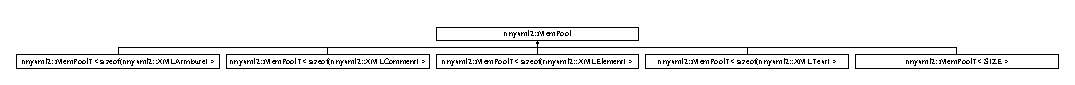
\includegraphics[height=0.691358cm]{classtinyxml2_1_1_mem_pool}
\end{center}
\end{figure}
\subsection*{Public Member Functions}
\begin{DoxyCompactItemize}
\item 
\hyperlink{classtinyxml2_1_1_mem_pool_a9101a0083d7370c85bd5aaaba7157f84}{Mem\+Pool} ()
\item 
virtual \hyperlink{classtinyxml2_1_1_mem_pool_ae55ad9e3faeca702e6ccbb38fdbcad72}{$\sim$\+Mem\+Pool} ()
\item 
virtual int \hyperlink{classtinyxml2_1_1_mem_pool_a0c518d49e3a94bde566f61e13b7240bb}{Item\+Size} () const =0
\item 
virtual void $\ast$ \hyperlink{classtinyxml2_1_1_mem_pool_a4f977b5fed752c0bbfe5295f469d6449}{Alloc} ()=0
\item 
virtual void \hyperlink{classtinyxml2_1_1_mem_pool_a49e3bfac2cba2ebd6776b31e571f64f7}{Free} (void $\ast$)=0
\item 
virtual void \hyperlink{classtinyxml2_1_1_mem_pool_ac5804dd1387b2e4de5eef710076a0db1}{Set\+Tracked} ()=0
\item 
virtual void \hyperlink{classtinyxml2_1_1_mem_pool_a74fcdef9756917c8ae19fbbb4d658ed7}{Clear} ()=0
\end{DoxyCompactItemize}


\subsection{Constructor \& Destructor Documentation}
\hypertarget{classtinyxml2_1_1_mem_pool_a9101a0083d7370c85bd5aaaba7157f84}{}\index{tinyxml2\+::\+Mem\+Pool@{tinyxml2\+::\+Mem\+Pool}!Mem\+Pool@{Mem\+Pool}}
\index{Mem\+Pool@{Mem\+Pool}!tinyxml2\+::\+Mem\+Pool@{tinyxml2\+::\+Mem\+Pool}}
\subsubsection[{Mem\+Pool}]{\setlength{\rightskip}{0pt plus 5cm}tinyxml2\+::\+Mem\+Pool\+::\+Mem\+Pool (
\begin{DoxyParamCaption}
{}
\end{DoxyParamCaption}
)\hspace{0.3cm}{\ttfamily [inline]}}\label{classtinyxml2_1_1_mem_pool_a9101a0083d7370c85bd5aaaba7157f84}
\hypertarget{classtinyxml2_1_1_mem_pool_ae55ad9e3faeca702e6ccbb38fdbcad72}{}\index{tinyxml2\+::\+Mem\+Pool@{tinyxml2\+::\+Mem\+Pool}!````~Mem\+Pool@{$\sim$\+Mem\+Pool}}
\index{````~Mem\+Pool@{$\sim$\+Mem\+Pool}!tinyxml2\+::\+Mem\+Pool@{tinyxml2\+::\+Mem\+Pool}}
\subsubsection[{$\sim$\+Mem\+Pool}]{\setlength{\rightskip}{0pt plus 5cm}virtual tinyxml2\+::\+Mem\+Pool\+::$\sim$\+Mem\+Pool (
\begin{DoxyParamCaption}
{}
\end{DoxyParamCaption}
)\hspace{0.3cm}{\ttfamily [inline]}, {\ttfamily [virtual]}}\label{classtinyxml2_1_1_mem_pool_ae55ad9e3faeca702e6ccbb38fdbcad72}


\subsection{Member Function Documentation}
\hypertarget{classtinyxml2_1_1_mem_pool_a4f977b5fed752c0bbfe5295f469d6449}{}\index{tinyxml2\+::\+Mem\+Pool@{tinyxml2\+::\+Mem\+Pool}!Alloc@{Alloc}}
\index{Alloc@{Alloc}!tinyxml2\+::\+Mem\+Pool@{tinyxml2\+::\+Mem\+Pool}}
\subsubsection[{Alloc}]{\setlength{\rightskip}{0pt plus 5cm}virtual void$\ast$ tinyxml2\+::\+Mem\+Pool\+::\+Alloc (
\begin{DoxyParamCaption}
{}
\end{DoxyParamCaption}
)\hspace{0.3cm}{\ttfamily [pure virtual]}}\label{classtinyxml2_1_1_mem_pool_a4f977b5fed752c0bbfe5295f469d6449}


Implemented in \hyperlink{classtinyxml2_1_1_mem_pool_t_aa9d785a48ffe6ea1be679bab13464486}{tinyxml2\+::\+Mem\+Pool\+T$<$ S\+I\+Z\+E $>$}, \hyperlink{classtinyxml2_1_1_mem_pool_t_aa9d785a48ffe6ea1be679bab13464486}{tinyxml2\+::\+Mem\+Pool\+T$<$ sizeof(tinyxml2\+::\+X\+M\+L\+Comment) $>$}, \hyperlink{classtinyxml2_1_1_mem_pool_t_aa9d785a48ffe6ea1be679bab13464486}{tinyxml2\+::\+Mem\+Pool\+T$<$ sizeof(tinyxml2\+::\+X\+M\+L\+Text) $>$}, \hyperlink{classtinyxml2_1_1_mem_pool_t_aa9d785a48ffe6ea1be679bab13464486}{tinyxml2\+::\+Mem\+Pool\+T$<$ sizeof(tinyxml2\+::\+X\+M\+L\+Attribute) $>$}, and \hyperlink{classtinyxml2_1_1_mem_pool_t_aa9d785a48ffe6ea1be679bab13464486}{tinyxml2\+::\+Mem\+Pool\+T$<$ sizeof(tinyxml2\+::\+X\+M\+L\+Element) $>$}.

\hypertarget{classtinyxml2_1_1_mem_pool_a74fcdef9756917c8ae19fbbb4d658ed7}{}\index{tinyxml2\+::\+Mem\+Pool@{tinyxml2\+::\+Mem\+Pool}!Clear@{Clear}}
\index{Clear@{Clear}!tinyxml2\+::\+Mem\+Pool@{tinyxml2\+::\+Mem\+Pool}}
\subsubsection[{Clear}]{\setlength{\rightskip}{0pt plus 5cm}virtual void tinyxml2\+::\+Mem\+Pool\+::\+Clear (
\begin{DoxyParamCaption}
{}
\end{DoxyParamCaption}
)\hspace{0.3cm}{\ttfamily [pure virtual]}}\label{classtinyxml2_1_1_mem_pool_a74fcdef9756917c8ae19fbbb4d658ed7}


Implemented in \hyperlink{classtinyxml2_1_1_mem_pool_t_a469d55e82be97d5ffeff82dd001a7029}{tinyxml2\+::\+Mem\+Pool\+T$<$ S\+I\+Z\+E $>$}, \hyperlink{classtinyxml2_1_1_mem_pool_t_a469d55e82be97d5ffeff82dd001a7029}{tinyxml2\+::\+Mem\+Pool\+T$<$ sizeof(tinyxml2\+::\+X\+M\+L\+Comment) $>$}, \hyperlink{classtinyxml2_1_1_mem_pool_t_a469d55e82be97d5ffeff82dd001a7029}{tinyxml2\+::\+Mem\+Pool\+T$<$ sizeof(tinyxml2\+::\+X\+M\+L\+Text) $>$}, \hyperlink{classtinyxml2_1_1_mem_pool_t_a469d55e82be97d5ffeff82dd001a7029}{tinyxml2\+::\+Mem\+Pool\+T$<$ sizeof(tinyxml2\+::\+X\+M\+L\+Attribute) $>$}, and \hyperlink{classtinyxml2_1_1_mem_pool_t_a469d55e82be97d5ffeff82dd001a7029}{tinyxml2\+::\+Mem\+Pool\+T$<$ sizeof(tinyxml2\+::\+X\+M\+L\+Element) $>$}.

\hypertarget{classtinyxml2_1_1_mem_pool_a49e3bfac2cba2ebd6776b31e571f64f7}{}\index{tinyxml2\+::\+Mem\+Pool@{tinyxml2\+::\+Mem\+Pool}!Free@{Free}}
\index{Free@{Free}!tinyxml2\+::\+Mem\+Pool@{tinyxml2\+::\+Mem\+Pool}}
\subsubsection[{Free}]{\setlength{\rightskip}{0pt plus 5cm}virtual void tinyxml2\+::\+Mem\+Pool\+::\+Free (
\begin{DoxyParamCaption}
\item[{void $\ast$}]{}
\end{DoxyParamCaption}
)\hspace{0.3cm}{\ttfamily [pure virtual]}}\label{classtinyxml2_1_1_mem_pool_a49e3bfac2cba2ebd6776b31e571f64f7}


Implemented in \hyperlink{classtinyxml2_1_1_mem_pool_t_a4f1a0c434e9e3d7391e5c16ed4ee8c70}{tinyxml2\+::\+Mem\+Pool\+T$<$ S\+I\+Z\+E $>$}, \hyperlink{classtinyxml2_1_1_mem_pool_t_a4f1a0c434e9e3d7391e5c16ed4ee8c70}{tinyxml2\+::\+Mem\+Pool\+T$<$ sizeof(tinyxml2\+::\+X\+M\+L\+Comment) $>$}, \hyperlink{classtinyxml2_1_1_mem_pool_t_a4f1a0c434e9e3d7391e5c16ed4ee8c70}{tinyxml2\+::\+Mem\+Pool\+T$<$ sizeof(tinyxml2\+::\+X\+M\+L\+Text) $>$}, \hyperlink{classtinyxml2_1_1_mem_pool_t_a4f1a0c434e9e3d7391e5c16ed4ee8c70}{tinyxml2\+::\+Mem\+Pool\+T$<$ sizeof(tinyxml2\+::\+X\+M\+L\+Attribute) $>$}, and \hyperlink{classtinyxml2_1_1_mem_pool_t_a4f1a0c434e9e3d7391e5c16ed4ee8c70}{tinyxml2\+::\+Mem\+Pool\+T$<$ sizeof(tinyxml2\+::\+X\+M\+L\+Element) $>$}.

\hypertarget{classtinyxml2_1_1_mem_pool_a0c518d49e3a94bde566f61e13b7240bb}{}\index{tinyxml2\+::\+Mem\+Pool@{tinyxml2\+::\+Mem\+Pool}!Item\+Size@{Item\+Size}}
\index{Item\+Size@{Item\+Size}!tinyxml2\+::\+Mem\+Pool@{tinyxml2\+::\+Mem\+Pool}}
\subsubsection[{Item\+Size}]{\setlength{\rightskip}{0pt plus 5cm}virtual int tinyxml2\+::\+Mem\+Pool\+::\+Item\+Size (
\begin{DoxyParamCaption}
{}
\end{DoxyParamCaption}
) const\hspace{0.3cm}{\ttfamily [pure virtual]}}\label{classtinyxml2_1_1_mem_pool_a0c518d49e3a94bde566f61e13b7240bb}


Implemented in \hyperlink{classtinyxml2_1_1_mem_pool_t_a7ec8778fe99f6e332615a703be0b48bc}{tinyxml2\+::\+Mem\+Pool\+T$<$ S\+I\+Z\+E $>$}, \hyperlink{classtinyxml2_1_1_mem_pool_t_a7ec8778fe99f6e332615a703be0b48bc}{tinyxml2\+::\+Mem\+Pool\+T$<$ sizeof(tinyxml2\+::\+X\+M\+L\+Comment) $>$}, \hyperlink{classtinyxml2_1_1_mem_pool_t_a7ec8778fe99f6e332615a703be0b48bc}{tinyxml2\+::\+Mem\+Pool\+T$<$ sizeof(tinyxml2\+::\+X\+M\+L\+Text) $>$}, \hyperlink{classtinyxml2_1_1_mem_pool_t_a7ec8778fe99f6e332615a703be0b48bc}{tinyxml2\+::\+Mem\+Pool\+T$<$ sizeof(tinyxml2\+::\+X\+M\+L\+Attribute) $>$}, and \hyperlink{classtinyxml2_1_1_mem_pool_t_a7ec8778fe99f6e332615a703be0b48bc}{tinyxml2\+::\+Mem\+Pool\+T$<$ sizeof(tinyxml2\+::\+X\+M\+L\+Element) $>$}.

\hypertarget{classtinyxml2_1_1_mem_pool_ac5804dd1387b2e4de5eef710076a0db1}{}\index{tinyxml2\+::\+Mem\+Pool@{tinyxml2\+::\+Mem\+Pool}!Set\+Tracked@{Set\+Tracked}}
\index{Set\+Tracked@{Set\+Tracked}!tinyxml2\+::\+Mem\+Pool@{tinyxml2\+::\+Mem\+Pool}}
\subsubsection[{Set\+Tracked}]{\setlength{\rightskip}{0pt plus 5cm}virtual void tinyxml2\+::\+Mem\+Pool\+::\+Set\+Tracked (
\begin{DoxyParamCaption}
{}
\end{DoxyParamCaption}
)\hspace{0.3cm}{\ttfamily [pure virtual]}}\label{classtinyxml2_1_1_mem_pool_ac5804dd1387b2e4de5eef710076a0db1}


Implemented in \hyperlink{classtinyxml2_1_1_mem_pool_t_a7798932414916199a1bc0f9c3f368521}{tinyxml2\+::\+Mem\+Pool\+T$<$ S\+I\+Z\+E $>$}, \hyperlink{classtinyxml2_1_1_mem_pool_t_a7798932414916199a1bc0f9c3f368521}{tinyxml2\+::\+Mem\+Pool\+T$<$ sizeof(tinyxml2\+::\+X\+M\+L\+Comment) $>$}, \hyperlink{classtinyxml2_1_1_mem_pool_t_a7798932414916199a1bc0f9c3f368521}{tinyxml2\+::\+Mem\+Pool\+T$<$ sizeof(tinyxml2\+::\+X\+M\+L\+Text) $>$}, \hyperlink{classtinyxml2_1_1_mem_pool_t_a7798932414916199a1bc0f9c3f368521}{tinyxml2\+::\+Mem\+Pool\+T$<$ sizeof(tinyxml2\+::\+X\+M\+L\+Attribute) $>$}, and \hyperlink{classtinyxml2_1_1_mem_pool_t_a7798932414916199a1bc0f9c3f368521}{tinyxml2\+::\+Mem\+Pool\+T$<$ sizeof(tinyxml2\+::\+X\+M\+L\+Element) $>$}.



The documentation for this class was generated from the following file\+:\begin{DoxyCompactItemize}
\item 
\hyperlink{tinyxml2_8h}{tinyxml2.\+h}\end{DoxyCompactItemize}

\hypertarget{classtinyxml2_1_1_mem_pool_t}{}\section{tinyxml2\+:\+:Mem\+Pool\+T$<$ S\+I\+Z\+E $>$ Class Template Reference}
\label{classtinyxml2_1_1_mem_pool_t}\index{tinyxml2\+::\+Mem\+Pool\+T$<$ S\+I\+Z\+E $>$@{tinyxml2\+::\+Mem\+Pool\+T$<$ S\+I\+Z\+E $>$}}


{\ttfamily \#include $<$tinyxml2.\+h$>$}

Inheritance diagram for tinyxml2\+:\+:Mem\+Pool\+T$<$ S\+I\+Z\+E $>$\+:\begin{figure}[H]
\begin{center}
\leavevmode
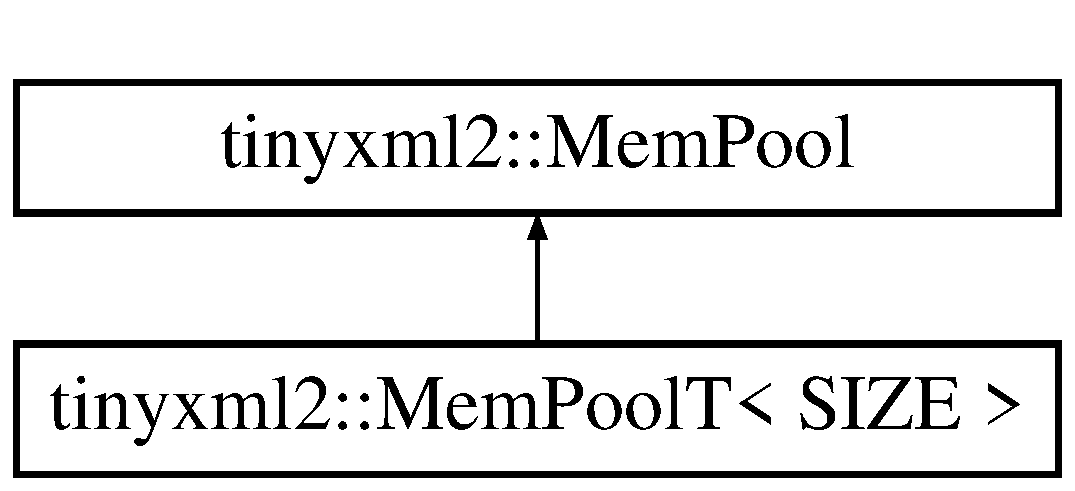
\includegraphics[height=2.000000cm]{classtinyxml2_1_1_mem_pool_t}
\end{center}
\end{figure}
\subsection*{Public Types}
\begin{DoxyCompactItemize}
\item 
enum \{ \hyperlink{classtinyxml2_1_1_mem_pool_t_a04cf45156e6f913f93972869ff8a1d94a4eeedbaa09fc9968120af6190e9e0988}{C\+O\+U\+N\+T} = (4$\ast$1024)/\+S\+I\+Z\+E
 \}
\end{DoxyCompactItemize}
\subsection*{Public Member Functions}
\begin{DoxyCompactItemize}
\item 
\hyperlink{classtinyxml2_1_1_mem_pool_t_a8a69a269ea72e292dde65309528ef64b}{Mem\+Pool\+T} ()
\item 
\hyperlink{classtinyxml2_1_1_mem_pool_t_ad6bb8346ad5b9a34f8f0051da5e3ed3f}{$\sim$\+Mem\+Pool\+T} ()
\item 
void \hyperlink{classtinyxml2_1_1_mem_pool_t_a469d55e82be97d5ffeff82dd001a7029}{Clear} ()
\item 
virtual int \hyperlink{classtinyxml2_1_1_mem_pool_t_a7ec8778fe99f6e332615a703be0b48bc}{Item\+Size} () const 
\item 
int \hyperlink{classtinyxml2_1_1_mem_pool_t_a56be11b7db6a7ef00db17088a7769aab}{Current\+Allocs} () const 
\item 
virtual void $\ast$ \hyperlink{classtinyxml2_1_1_mem_pool_t_aa9d785a48ffe6ea1be679bab13464486}{Alloc} ()
\item 
virtual void \hyperlink{classtinyxml2_1_1_mem_pool_t_a4f1a0c434e9e3d7391e5c16ed4ee8c70}{Free} (void $\ast$mem)
\item 
void \hyperlink{classtinyxml2_1_1_mem_pool_t_a0bc596f271e0f139822c534238b3f244}{Trace} (const char $\ast$name)
\item 
void \hyperlink{classtinyxml2_1_1_mem_pool_t_a7798932414916199a1bc0f9c3f368521}{Set\+Tracked} ()
\item 
int \hyperlink{classtinyxml2_1_1_mem_pool_t_a524b90d0edeac41964c06510757dce0f}{Untracked} () const 
\end{DoxyCompactItemize}


\subsection{Member Enumeration Documentation}
\hypertarget{classtinyxml2_1_1_mem_pool_t_a04cf45156e6f913f93972869ff8a1d94}{}\subsubsection[{anonymous enum}]{\setlength{\rightskip}{0pt plus 5cm}template$<$int S\+I\+Z\+E$>$ anonymous enum}\label{classtinyxml2_1_1_mem_pool_t_a04cf45156e6f913f93972869ff8a1d94}
\begin{Desc}
\item[Enumerator]\par
\begin{description}
\index{C\+O\+U\+N\+T@{C\+O\+U\+N\+T}!tinyxml2\+::\+Mem\+Pool\+T@{tinyxml2\+::\+Mem\+Pool\+T}}\index{tinyxml2\+::\+Mem\+Pool\+T@{tinyxml2\+::\+Mem\+Pool\+T}!C\+O\+U\+N\+T@{C\+O\+U\+N\+T}}\item[{\em 
\hypertarget{classtinyxml2_1_1_mem_pool_t_a04cf45156e6f913f93972869ff8a1d94a4eeedbaa09fc9968120af6190e9e0988}{}C\+O\+U\+N\+T\label{classtinyxml2_1_1_mem_pool_t_a04cf45156e6f913f93972869ff8a1d94a4eeedbaa09fc9968120af6190e9e0988}
}]\end{description}
\end{Desc}


\subsection{Constructor \& Destructor Documentation}
\hypertarget{classtinyxml2_1_1_mem_pool_t_a8a69a269ea72e292dde65309528ef64b}{}\index{tinyxml2\+::\+Mem\+Pool\+T@{tinyxml2\+::\+Mem\+Pool\+T}!Mem\+Pool\+T@{Mem\+Pool\+T}}
\index{Mem\+Pool\+T@{Mem\+Pool\+T}!tinyxml2\+::\+Mem\+Pool\+T@{tinyxml2\+::\+Mem\+Pool\+T}}
\subsubsection[{Mem\+Pool\+T}]{\setlength{\rightskip}{0pt plus 5cm}template$<$int S\+I\+Z\+E$>$ {\bf tinyxml2\+::\+Mem\+Pool\+T}$<$ S\+I\+Z\+E $>$\+::{\bf Mem\+Pool\+T} (
\begin{DoxyParamCaption}
{}
\end{DoxyParamCaption}
)\hspace{0.3cm}{\ttfamily [inline]}}\label{classtinyxml2_1_1_mem_pool_t_a8a69a269ea72e292dde65309528ef64b}
\hypertarget{classtinyxml2_1_1_mem_pool_t_ad6bb8346ad5b9a34f8f0051da5e3ed3f}{}\index{tinyxml2\+::\+Mem\+Pool\+T@{tinyxml2\+::\+Mem\+Pool\+T}!````~Mem\+Pool\+T@{$\sim$\+Mem\+Pool\+T}}
\index{````~Mem\+Pool\+T@{$\sim$\+Mem\+Pool\+T}!tinyxml2\+::\+Mem\+Pool\+T@{tinyxml2\+::\+Mem\+Pool\+T}}
\subsubsection[{$\sim$\+Mem\+Pool\+T}]{\setlength{\rightskip}{0pt plus 5cm}template$<$int S\+I\+Z\+E$>$ {\bf tinyxml2\+::\+Mem\+Pool\+T}$<$ S\+I\+Z\+E $>$\+::$\sim${\bf Mem\+Pool\+T} (
\begin{DoxyParamCaption}
{}
\end{DoxyParamCaption}
)\hspace{0.3cm}{\ttfamily [inline]}}\label{classtinyxml2_1_1_mem_pool_t_ad6bb8346ad5b9a34f8f0051da5e3ed3f}


\subsection{Member Function Documentation}
\hypertarget{classtinyxml2_1_1_mem_pool_t_aa9d785a48ffe6ea1be679bab13464486}{}\index{tinyxml2\+::\+Mem\+Pool\+T@{tinyxml2\+::\+Mem\+Pool\+T}!Alloc@{Alloc}}
\index{Alloc@{Alloc}!tinyxml2\+::\+Mem\+Pool\+T@{tinyxml2\+::\+Mem\+Pool\+T}}
\subsubsection[{Alloc}]{\setlength{\rightskip}{0pt plus 5cm}template$<$int S\+I\+Z\+E$>$ virtual void$\ast$ {\bf tinyxml2\+::\+Mem\+Pool\+T}$<$ S\+I\+Z\+E $>$\+::Alloc (
\begin{DoxyParamCaption}
{}
\end{DoxyParamCaption}
)\hspace{0.3cm}{\ttfamily [inline]}, {\ttfamily [virtual]}}\label{classtinyxml2_1_1_mem_pool_t_aa9d785a48ffe6ea1be679bab13464486}


Implements \hyperlink{classtinyxml2_1_1_mem_pool_a4f977b5fed752c0bbfe5295f469d6449}{tinyxml2\+::\+Mem\+Pool}.

\hypertarget{classtinyxml2_1_1_mem_pool_t_a469d55e82be97d5ffeff82dd001a7029}{}\index{tinyxml2\+::\+Mem\+Pool\+T@{tinyxml2\+::\+Mem\+Pool\+T}!Clear@{Clear}}
\index{Clear@{Clear}!tinyxml2\+::\+Mem\+Pool\+T@{tinyxml2\+::\+Mem\+Pool\+T}}
\subsubsection[{Clear}]{\setlength{\rightskip}{0pt plus 5cm}template$<$int S\+I\+Z\+E$>$ void {\bf tinyxml2\+::\+Mem\+Pool\+T}$<$ S\+I\+Z\+E $>$\+::Clear (
\begin{DoxyParamCaption}
{}
\end{DoxyParamCaption}
)\hspace{0.3cm}{\ttfamily [inline]}, {\ttfamily [virtual]}}\label{classtinyxml2_1_1_mem_pool_t_a469d55e82be97d5ffeff82dd001a7029}


Implements \hyperlink{classtinyxml2_1_1_mem_pool_a74fcdef9756917c8ae19fbbb4d658ed7}{tinyxml2\+::\+Mem\+Pool}.

\hypertarget{classtinyxml2_1_1_mem_pool_t_a56be11b7db6a7ef00db17088a7769aab}{}\index{tinyxml2\+::\+Mem\+Pool\+T@{tinyxml2\+::\+Mem\+Pool\+T}!Current\+Allocs@{Current\+Allocs}}
\index{Current\+Allocs@{Current\+Allocs}!tinyxml2\+::\+Mem\+Pool\+T@{tinyxml2\+::\+Mem\+Pool\+T}}
\subsubsection[{Current\+Allocs}]{\setlength{\rightskip}{0pt plus 5cm}template$<$int S\+I\+Z\+E$>$ int {\bf tinyxml2\+::\+Mem\+Pool\+T}$<$ S\+I\+Z\+E $>$\+::Current\+Allocs (
\begin{DoxyParamCaption}
{}
\end{DoxyParamCaption}
) const\hspace{0.3cm}{\ttfamily [inline]}}\label{classtinyxml2_1_1_mem_pool_t_a56be11b7db6a7ef00db17088a7769aab}
\hypertarget{classtinyxml2_1_1_mem_pool_t_a4f1a0c434e9e3d7391e5c16ed4ee8c70}{}\index{tinyxml2\+::\+Mem\+Pool\+T@{tinyxml2\+::\+Mem\+Pool\+T}!Free@{Free}}
\index{Free@{Free}!tinyxml2\+::\+Mem\+Pool\+T@{tinyxml2\+::\+Mem\+Pool\+T}}
\subsubsection[{Free}]{\setlength{\rightskip}{0pt plus 5cm}template$<$int S\+I\+Z\+E$>$ virtual void {\bf tinyxml2\+::\+Mem\+Pool\+T}$<$ S\+I\+Z\+E $>$\+::Free (
\begin{DoxyParamCaption}
\item[{void $\ast$}]{mem}
\end{DoxyParamCaption}
)\hspace{0.3cm}{\ttfamily [inline]}, {\ttfamily [virtual]}}\label{classtinyxml2_1_1_mem_pool_t_a4f1a0c434e9e3d7391e5c16ed4ee8c70}


Implements \hyperlink{classtinyxml2_1_1_mem_pool_a49e3bfac2cba2ebd6776b31e571f64f7}{tinyxml2\+::\+Mem\+Pool}.

\hypertarget{classtinyxml2_1_1_mem_pool_t_a7ec8778fe99f6e332615a703be0b48bc}{}\index{tinyxml2\+::\+Mem\+Pool\+T@{tinyxml2\+::\+Mem\+Pool\+T}!Item\+Size@{Item\+Size}}
\index{Item\+Size@{Item\+Size}!tinyxml2\+::\+Mem\+Pool\+T@{tinyxml2\+::\+Mem\+Pool\+T}}
\subsubsection[{Item\+Size}]{\setlength{\rightskip}{0pt plus 5cm}template$<$int S\+I\+Z\+E$>$ virtual int {\bf tinyxml2\+::\+Mem\+Pool\+T}$<$ S\+I\+Z\+E $>$\+::Item\+Size (
\begin{DoxyParamCaption}
{}
\end{DoxyParamCaption}
) const\hspace{0.3cm}{\ttfamily [inline]}, {\ttfamily [virtual]}}\label{classtinyxml2_1_1_mem_pool_t_a7ec8778fe99f6e332615a703be0b48bc}


Implements \hyperlink{classtinyxml2_1_1_mem_pool_a0c518d49e3a94bde566f61e13b7240bb}{tinyxml2\+::\+Mem\+Pool}.

\hypertarget{classtinyxml2_1_1_mem_pool_t_a7798932414916199a1bc0f9c3f368521}{}\index{tinyxml2\+::\+Mem\+Pool\+T@{tinyxml2\+::\+Mem\+Pool\+T}!Set\+Tracked@{Set\+Tracked}}
\index{Set\+Tracked@{Set\+Tracked}!tinyxml2\+::\+Mem\+Pool\+T@{tinyxml2\+::\+Mem\+Pool\+T}}
\subsubsection[{Set\+Tracked}]{\setlength{\rightskip}{0pt plus 5cm}template$<$int S\+I\+Z\+E$>$ void {\bf tinyxml2\+::\+Mem\+Pool\+T}$<$ S\+I\+Z\+E $>$\+::Set\+Tracked (
\begin{DoxyParamCaption}
{}
\end{DoxyParamCaption}
)\hspace{0.3cm}{\ttfamily [inline]}, {\ttfamily [virtual]}}\label{classtinyxml2_1_1_mem_pool_t_a7798932414916199a1bc0f9c3f368521}


Implements \hyperlink{classtinyxml2_1_1_mem_pool_ac5804dd1387b2e4de5eef710076a0db1}{tinyxml2\+::\+Mem\+Pool}.

\hypertarget{classtinyxml2_1_1_mem_pool_t_a0bc596f271e0f139822c534238b3f244}{}\index{tinyxml2\+::\+Mem\+Pool\+T@{tinyxml2\+::\+Mem\+Pool\+T}!Trace@{Trace}}
\index{Trace@{Trace}!tinyxml2\+::\+Mem\+Pool\+T@{tinyxml2\+::\+Mem\+Pool\+T}}
\subsubsection[{Trace}]{\setlength{\rightskip}{0pt plus 5cm}template$<$int S\+I\+Z\+E$>$ void {\bf tinyxml2\+::\+Mem\+Pool\+T}$<$ S\+I\+Z\+E $>$\+::Trace (
\begin{DoxyParamCaption}
\item[{const char $\ast$}]{name}
\end{DoxyParamCaption}
)\hspace{0.3cm}{\ttfamily [inline]}}\label{classtinyxml2_1_1_mem_pool_t_a0bc596f271e0f139822c534238b3f244}
\hypertarget{classtinyxml2_1_1_mem_pool_t_a524b90d0edeac41964c06510757dce0f}{}\index{tinyxml2\+::\+Mem\+Pool\+T@{tinyxml2\+::\+Mem\+Pool\+T}!Untracked@{Untracked}}
\index{Untracked@{Untracked}!tinyxml2\+::\+Mem\+Pool\+T@{tinyxml2\+::\+Mem\+Pool\+T}}
\subsubsection[{Untracked}]{\setlength{\rightskip}{0pt plus 5cm}template$<$int S\+I\+Z\+E$>$ int {\bf tinyxml2\+::\+Mem\+Pool\+T}$<$ S\+I\+Z\+E $>$\+::Untracked (
\begin{DoxyParamCaption}
{}
\end{DoxyParamCaption}
) const\hspace{0.3cm}{\ttfamily [inline]}}\label{classtinyxml2_1_1_mem_pool_t_a524b90d0edeac41964c06510757dce0f}


The documentation for this class was generated from the following file\+:\begin{DoxyCompactItemize}
\item 
\hyperlink{tinyxml2_8h}{tinyxml2.\+h}\end{DoxyCompactItemize}

\hypertarget{class_quad}{}\section{Quad Class Reference}
\label{class_quad}\index{Quad@{Quad}}


creates verticies and shaders for quad and stores them in the V\+B\+O  




{\ttfamily \#include $<$quad.\+h$>$}

\subsection*{Public Member Functions}
\begin{DoxyCompactItemize}
\item 
\hyperlink{class_quad_ae446d188d645cc5c512336f25d1a697a}{Quad} ()
\item 
void \hyperlink{class_quad_a4febbb07741319565e1ee7abe8ab4674}{Draw} ()
\begin{DoxyCompactList}\small\item\em enables shader program, vertex data, and texture to draw quad. \end{DoxyCompactList}\item 
\hyperlink{class_quad_a5db77c0481b30c0b7c1014cc535284ad}{$\sim$\+Quad} ()
\end{DoxyCompactItemize}
\subsection*{Public Attributes}
\begin{DoxyCompactItemize}
\item 
G\+Luint \hyperlink{class_quad_af710bcaf3209f47cb75dfed003604fd4}{V\+B\+O}
\begin{DoxyCompactList}\small\item\em \hyperlink{struct_vertex}{Vertex} Buffer Object to store quad data. \end{DoxyCompactList}\item 
\hyperlink{struct_vertex}{Vertex} \hyperlink{class_quad_afaed261444ab07e840d903baff5c0624}{rect} \mbox{[}4\mbox{]}
\begin{DoxyCompactList}\small\item\em vertex array that holds vertex data \end{DoxyCompactList}\item 
G\+Luint \hyperlink{class_quad_a04b4a7628b803cdedfac290a26e97f75}{ui\+Texture\+Id}
\begin{DoxyCompactList}\small\item\em quad\textquotesingle{}s texture id \end{DoxyCompactList}\item 
\hyperlink{_sprite_8h_a2db59f395fe82a7394c6324956c265d8}{glm\+::mat4} \hyperlink{class_quad_a412bc084a6c764c235b546be5fc4a7b6}{M\+V\+P}
\item 
\hyperlink{_sprite_8h_a2db59f395fe82a7394c6324956c265d8}{glm\+::mat4} \hyperlink{class_quad_a31981a73c8503bf906450ab2caadd32b}{Model}
\item 
\hyperlink{_sprite_8h_a2db59f395fe82a7394c6324956c265d8}{glm\+::mat4} \hyperlink{class_quad_a25e399068755865ba1e2c25d01837863}{View}
\begin{DoxyCompactList}\small\item\em matricies for matrix math \end{DoxyCompactList}\item 
\hyperlink{_sprite_8h_a3d0ce73e3199de81565fb01632415288}{glm\+::vec3} \hyperlink{class_quad_a71b5296b41053bfc400e08c579997c0f}{m\+\_\+transate}
\item 
\hyperlink{_sprite_8h_a3d0ce73e3199de81565fb01632415288}{glm\+::vec3} \hyperlink{class_quad_a94d9fe0e5fa32916ab80f263a3dc43b4}{m\+\_\+scale}
\item 
\hyperlink{_sprite_8h_a3d0ce73e3199de81565fb01632415288}{glm\+::vec3} \hyperlink{class_quad_a0f056585749e1e4af52ea80c9e450353}{m\+\_\+rotate}
\begin{DoxyCompactList}\small\item\em vectors for transform math \end{DoxyCompactList}\end{DoxyCompactItemize}


\subsection{Detailed Description}
creates verticies and shaders for quad and stores them in the V\+B\+O 

\subsection{Constructor \& Destructor Documentation}
\hypertarget{class_quad_ae446d188d645cc5c512336f25d1a697a}{}\index{Quad@{Quad}!Quad@{Quad}}
\index{Quad@{Quad}!Quad@{Quad}}
\subsubsection[{Quad}]{\setlength{\rightskip}{0pt plus 5cm}Quad\+::\+Quad (
\begin{DoxyParamCaption}
{}
\end{DoxyParamCaption}
)}\label{class_quad_ae446d188d645cc5c512336f25d1a697a}
\hypertarget{class_quad_a5db77c0481b30c0b7c1014cc535284ad}{}\index{Quad@{Quad}!````~Quad@{$\sim$\+Quad}}
\index{````~Quad@{$\sim$\+Quad}!Quad@{Quad}}
\subsubsection[{$\sim$\+Quad}]{\setlength{\rightskip}{0pt plus 5cm}Quad\+::$\sim$\+Quad (
\begin{DoxyParamCaption}
{}
\end{DoxyParamCaption}
)\hspace{0.3cm}{\ttfamily [inline]}}\label{class_quad_a5db77c0481b30c0b7c1014cc535284ad}


\subsection{Member Function Documentation}
\hypertarget{class_quad_a4febbb07741319565e1ee7abe8ab4674}{}\index{Quad@{Quad}!Draw@{Draw}}
\index{Draw@{Draw}!Quad@{Quad}}
\subsubsection[{Draw}]{\setlength{\rightskip}{0pt plus 5cm}void Quad\+::\+Draw (
\begin{DoxyParamCaption}
{}
\end{DoxyParamCaption}
)}\label{class_quad_a4febbb07741319565e1ee7abe8ab4674}


enables shader program, vertex data, and texture to draw quad. 



\subsection{Member Data Documentation}
\hypertarget{class_quad_a0f056585749e1e4af52ea80c9e450353}{}\index{Quad@{Quad}!m\+\_\+rotate@{m\+\_\+rotate}}
\index{m\+\_\+rotate@{m\+\_\+rotate}!Quad@{Quad}}
\subsubsection[{m\+\_\+rotate}]{\setlength{\rightskip}{0pt plus 5cm}{\bf glm\+::vec3} Quad\+::m\+\_\+rotate}\label{class_quad_a0f056585749e1e4af52ea80c9e450353}


vectors for transform math 

\hypertarget{class_quad_a94d9fe0e5fa32916ab80f263a3dc43b4}{}\index{Quad@{Quad}!m\+\_\+scale@{m\+\_\+scale}}
\index{m\+\_\+scale@{m\+\_\+scale}!Quad@{Quad}}
\subsubsection[{m\+\_\+scale}]{\setlength{\rightskip}{0pt plus 5cm}{\bf glm\+::vec3} Quad\+::m\+\_\+scale}\label{class_quad_a94d9fe0e5fa32916ab80f263a3dc43b4}
\hypertarget{class_quad_a71b5296b41053bfc400e08c579997c0f}{}\index{Quad@{Quad}!m\+\_\+transate@{m\+\_\+transate}}
\index{m\+\_\+transate@{m\+\_\+transate}!Quad@{Quad}}
\subsubsection[{m\+\_\+transate}]{\setlength{\rightskip}{0pt plus 5cm}{\bf glm\+::vec3} Quad\+::m\+\_\+transate}\label{class_quad_a71b5296b41053bfc400e08c579997c0f}
\hypertarget{class_quad_a31981a73c8503bf906450ab2caadd32b}{}\index{Quad@{Quad}!Model@{Model}}
\index{Model@{Model}!Quad@{Quad}}
\subsubsection[{Model}]{\setlength{\rightskip}{0pt plus 5cm}{\bf glm\+::mat4} Quad\+::\+Model}\label{class_quad_a31981a73c8503bf906450ab2caadd32b}
\hypertarget{class_quad_a412bc084a6c764c235b546be5fc4a7b6}{}\index{Quad@{Quad}!M\+V\+P@{M\+V\+P}}
\index{M\+V\+P@{M\+V\+P}!Quad@{Quad}}
\subsubsection[{M\+V\+P}]{\setlength{\rightskip}{0pt plus 5cm}{\bf glm\+::mat4} Quad\+::\+M\+V\+P}\label{class_quad_a412bc084a6c764c235b546be5fc4a7b6}
\hypertarget{class_quad_afaed261444ab07e840d903baff5c0624}{}\index{Quad@{Quad}!rect@{rect}}
\index{rect@{rect}!Quad@{Quad}}
\subsubsection[{rect}]{\setlength{\rightskip}{0pt plus 5cm}{\bf Vertex} Quad\+::rect\mbox{[}4\mbox{]}}\label{class_quad_afaed261444ab07e840d903baff5c0624}


vertex array that holds vertex data 

\hypertarget{class_quad_a04b4a7628b803cdedfac290a26e97f75}{}\index{Quad@{Quad}!ui\+Texture\+Id@{ui\+Texture\+Id}}
\index{ui\+Texture\+Id@{ui\+Texture\+Id}!Quad@{Quad}}
\subsubsection[{ui\+Texture\+Id}]{\setlength{\rightskip}{0pt plus 5cm}G\+Luint Quad\+::ui\+Texture\+Id}\label{class_quad_a04b4a7628b803cdedfac290a26e97f75}


quad\textquotesingle{}s texture id 

\hypertarget{class_quad_af710bcaf3209f47cb75dfed003604fd4}{}\index{Quad@{Quad}!V\+B\+O@{V\+B\+O}}
\index{V\+B\+O@{V\+B\+O}!Quad@{Quad}}
\subsubsection[{V\+B\+O}]{\setlength{\rightskip}{0pt plus 5cm}G\+Luint Quad\+::\+V\+B\+O}\label{class_quad_af710bcaf3209f47cb75dfed003604fd4}


\hyperlink{struct_vertex}{Vertex} Buffer Object to store quad data. 

\hypertarget{class_quad_a25e399068755865ba1e2c25d01837863}{}\index{Quad@{Quad}!View@{View}}
\index{View@{View}!Quad@{Quad}}
\subsubsection[{View}]{\setlength{\rightskip}{0pt plus 5cm}{\bf glm\+::mat4} Quad\+::\+View}\label{class_quad_a25e399068755865ba1e2c25d01837863}


matricies for matrix math 



The documentation for this class was generated from the following files\+:\begin{DoxyCompactItemize}
\item 
\hyperlink{quad_8h}{quad.\+h}\item 
\hyperlink{quad_8cpp}{quad.\+cpp}\end{DoxyCompactItemize}

\hypertarget{class_sprite}{}\section{Sprite Class Reference}
\label{class_sprite}\index{Sprite@{Sprite}}


reads and creates texture for a quad  




{\ttfamily \#include $<$Sprite.\+h$>$}

\subsection*{Public Member Functions}
\begin{DoxyCompactItemize}
\item 
\hyperlink{class_sprite_a12cba3ac1868418add3c4d95ce87e615}{Sprite} ()
\item 
void \hyperlink{class_sprite_ad9cb3e4978cec898aedcc0126642e2d2}{Create\+Sprite} (const char $\ast$filename)
\begin{DoxyCompactList}\small\item\em enables shader program, vertex data, and texture to draw quad \end{DoxyCompactList}\item 
void \hyperlink{class_sprite_a550265943afb5e79fd76f1c163fb9415}{Set\+U\+Vs} (unsigned int sprite\+Id, float top\+X, float top\+Y, float bottom\+X, float bottom\+Y)
\begin{DoxyCompactList}\small\item\em sets the uvs of the texture being used \end{DoxyCompactList}\item 
void \hyperlink{class_sprite_a054a4c340c14c3d218b99e484bf83d21}{Draw} ()
\begin{DoxyCompactList}\small\item\em calls quad.\+draw() \end{DoxyCompactList}\item 
void \hyperlink{class_sprite_aa803a9eae66b98130f2ef589db24692a}{Move\+Sprite} (float x, float y)
\begin{DoxyCompactList}\small\item\em ability to adjust the x position adn y position of sprite \end{DoxyCompactList}\item 
void \hyperlink{class_sprite_acf9da4f7a3caf15004f69c9bcc696b5c}{Scale\+Sprite} (float x, float y)
\item 
void \hyperlink{class_sprite_a7f4858ef8ab1aa9caf60522b6c89cf9c}{Adjust\+Sprite} ()
\item 
\hyperlink{class_sprite_a8accab430f9d90ae5117b57d67e32b84}{$\sim$\+Sprite} ()
\end{DoxyCompactItemize}
\subsection*{Public Attributes}
\begin{DoxyCompactItemize}
\item 
\hyperlink{class_quad}{Quad} \hyperlink{class_sprite_a263d37687035ace0db0909f0090dad45}{Sprite\+Quad}
\begin{DoxyCompactList}\small\item\em creates quad to attach texture \end{DoxyCompactList}\end{DoxyCompactItemize}


\subsection{Detailed Description}
reads and creates texture for a quad 

\subsection{Constructor \& Destructor Documentation}
\hypertarget{class_sprite_a12cba3ac1868418add3c4d95ce87e615}{}\index{Sprite@{Sprite}!Sprite@{Sprite}}
\index{Sprite@{Sprite}!Sprite@{Sprite}}
\subsubsection[{Sprite}]{\setlength{\rightskip}{0pt plus 5cm}Sprite\+::\+Sprite (
\begin{DoxyParamCaption}
{}
\end{DoxyParamCaption}
)\hspace{0.3cm}{\ttfamily [inline]}}\label{class_sprite_a12cba3ac1868418add3c4d95ce87e615}
\hypertarget{class_sprite_a8accab430f9d90ae5117b57d67e32b84}{}\index{Sprite@{Sprite}!````~Sprite@{$\sim$\+Sprite}}
\index{````~Sprite@{$\sim$\+Sprite}!Sprite@{Sprite}}
\subsubsection[{$\sim$\+Sprite}]{\setlength{\rightskip}{0pt plus 5cm}Sprite\+::$\sim$\+Sprite (
\begin{DoxyParamCaption}
{}
\end{DoxyParamCaption}
)\hspace{0.3cm}{\ttfamily [inline]}}\label{class_sprite_a8accab430f9d90ae5117b57d67e32b84}


\subsection{Member Function Documentation}
\hypertarget{class_sprite_a7f4858ef8ab1aa9caf60522b6c89cf9c}{}\index{Sprite@{Sprite}!Adjust\+Sprite@{Adjust\+Sprite}}
\index{Adjust\+Sprite@{Adjust\+Sprite}!Sprite@{Sprite}}
\subsubsection[{Adjust\+Sprite}]{\setlength{\rightskip}{0pt plus 5cm}void Sprite\+::\+Adjust\+Sprite (
\begin{DoxyParamCaption}
{}
\end{DoxyParamCaption}
)}\label{class_sprite_a7f4858ef8ab1aa9caf60522b6c89cf9c}
\hypertarget{class_sprite_ad9cb3e4978cec898aedcc0126642e2d2}{}\index{Sprite@{Sprite}!Create\+Sprite@{Create\+Sprite}}
\index{Create\+Sprite@{Create\+Sprite}!Sprite@{Sprite}}
\subsubsection[{Create\+Sprite}]{\setlength{\rightskip}{0pt plus 5cm}void Sprite\+::\+Create\+Sprite (
\begin{DoxyParamCaption}
\item[{const char $\ast$}]{filename}
\end{DoxyParamCaption}
)}\label{class_sprite_ad9cb3e4978cec898aedcc0126642e2d2}


enables shader program, vertex data, and texture to draw quad 


\begin{DoxyParams}{Parameters}
{\em file} & name of texture \\
\hline
\end{DoxyParams}
\hypertarget{class_sprite_a054a4c340c14c3d218b99e484bf83d21}{}\index{Sprite@{Sprite}!Draw@{Draw}}
\index{Draw@{Draw}!Sprite@{Sprite}}
\subsubsection[{Draw}]{\setlength{\rightskip}{0pt plus 5cm}void Sprite\+::\+Draw (
\begin{DoxyParamCaption}
{}
\end{DoxyParamCaption}
)}\label{class_sprite_a054a4c340c14c3d218b99e484bf83d21}


calls quad.\+draw() 

\hypertarget{class_sprite_aa803a9eae66b98130f2ef589db24692a}{}\index{Sprite@{Sprite}!Move\+Sprite@{Move\+Sprite}}
\index{Move\+Sprite@{Move\+Sprite}!Sprite@{Sprite}}
\subsubsection[{Move\+Sprite}]{\setlength{\rightskip}{0pt plus 5cm}void Sprite\+::\+Move\+Sprite (
\begin{DoxyParamCaption}
\item[{float}]{x, }
\item[{float}]{y}
\end{DoxyParamCaption}
)}\label{class_sprite_aa803a9eae66b98130f2ef589db24692a}


ability to adjust the x position adn y position of sprite 


\begin{DoxyParams}{Parameters}
{\em x} & and y translation \\
\hline
\end{DoxyParams}
\hypertarget{class_sprite_acf9da4f7a3caf15004f69c9bcc696b5c}{}\index{Sprite@{Sprite}!Scale\+Sprite@{Scale\+Sprite}}
\index{Scale\+Sprite@{Scale\+Sprite}!Sprite@{Sprite}}
\subsubsection[{Scale\+Sprite}]{\setlength{\rightskip}{0pt plus 5cm}void Sprite\+::\+Scale\+Sprite (
\begin{DoxyParamCaption}
\item[{float}]{x, }
\item[{float}]{y}
\end{DoxyParamCaption}
)}\label{class_sprite_acf9da4f7a3caf15004f69c9bcc696b5c}
\hypertarget{class_sprite_a550265943afb5e79fd76f1c163fb9415}{}\index{Sprite@{Sprite}!Set\+U\+Vs@{Set\+U\+Vs}}
\index{Set\+U\+Vs@{Set\+U\+Vs}!Sprite@{Sprite}}
\subsubsection[{Set\+U\+Vs}]{\setlength{\rightskip}{0pt plus 5cm}void Sprite\+::\+Set\+U\+Vs (
\begin{DoxyParamCaption}
\item[{unsigned int}]{sprite\+Id, }
\item[{float}]{top\+X, }
\item[{float}]{top\+Y, }
\item[{float}]{bottom\+X, }
\item[{float}]{bottom\+Y}
\end{DoxyParamCaption}
)}\label{class_sprite_a550265943afb5e79fd76f1c163fb9415}


sets the uvs of the texture being used 


\begin{DoxyParams}{Parameters}
{\em sprite\+I\+D,top} & x and y, bottom x and y \\
\hline
\end{DoxyParams}


\subsection{Member Data Documentation}
\hypertarget{class_sprite_a263d37687035ace0db0909f0090dad45}{}\index{Sprite@{Sprite}!Sprite\+Quad@{Sprite\+Quad}}
\index{Sprite\+Quad@{Sprite\+Quad}!Sprite@{Sprite}}
\subsubsection[{Sprite\+Quad}]{\setlength{\rightskip}{0pt plus 5cm}{\bf Quad} Sprite\+::\+Sprite\+Quad}\label{class_sprite_a263d37687035ace0db0909f0090dad45}


creates quad to attach texture 



The documentation for this class was generated from the following files\+:\begin{DoxyCompactItemize}
\item 
\hyperlink{_sprite_8h}{Sprite.\+h}\item 
\hyperlink{_sprite_8cpp}{Sprite.\+cpp}\end{DoxyCompactItemize}

\hypertarget{struct_sprite_data}{}\section{Sprite\+Data Struct Reference}
\label{struct_sprite_data}\index{Sprite\+Data@{Sprite\+Data}}


holds sprite U\+V data  




{\ttfamily \#include $<$Animator.\+h$>$}

\subsection*{Public Attributes}
\begin{DoxyCompactItemize}
\item 
unsigned int \hyperlink{struct_sprite_data_a0e22de2e782f60b1ffb5697cf72824cd}{id}
\begin{DoxyCompactList}\small\item\em sprite i\+D \end{DoxyCompactList}\item 
float \hyperlink{struct_sprite_data_a726087f7ea88f2cd8c0841e2c3923628}{x0}
\item 
float \hyperlink{struct_sprite_data_a8c06fce0212a7a8358d59670cf77210b}{y0}
\item 
float \hyperlink{struct_sprite_data_a0dda77ba2d31603e1a71c9b76c5db221}{x1}
\item 
float \hyperlink{struct_sprite_data_a90665db5ae717daab6bcb2726f3fab50}{y1}
\begin{DoxyCompactList}\small\item\em uvs \end{DoxyCompactList}\item 
const char $\ast$ \hyperlink{struct_sprite_data_a942d4fe5b3d2cb84315282ad34e3f64f}{name}
\begin{DoxyCompactList}\small\item\em sprite name \end{DoxyCompactList}\end{DoxyCompactItemize}


\subsection{Detailed Description}
holds sprite U\+V data 

\subsection{Member Data Documentation}
\hypertarget{struct_sprite_data_a0e22de2e782f60b1ffb5697cf72824cd}{}\index{Sprite\+Data@{Sprite\+Data}!id@{id}}
\index{id@{id}!Sprite\+Data@{Sprite\+Data}}
\subsubsection[{id}]{\setlength{\rightskip}{0pt plus 5cm}unsigned int Sprite\+Data\+::id}\label{struct_sprite_data_a0e22de2e782f60b1ffb5697cf72824cd}


sprite i\+D 

\hypertarget{struct_sprite_data_a942d4fe5b3d2cb84315282ad34e3f64f}{}\index{Sprite\+Data@{Sprite\+Data}!name@{name}}
\index{name@{name}!Sprite\+Data@{Sprite\+Data}}
\subsubsection[{name}]{\setlength{\rightskip}{0pt plus 5cm}const char$\ast$ Sprite\+Data\+::name}\label{struct_sprite_data_a942d4fe5b3d2cb84315282ad34e3f64f}


sprite name 

\hypertarget{struct_sprite_data_a726087f7ea88f2cd8c0841e2c3923628}{}\index{Sprite\+Data@{Sprite\+Data}!x0@{x0}}
\index{x0@{x0}!Sprite\+Data@{Sprite\+Data}}
\subsubsection[{x0}]{\setlength{\rightskip}{0pt plus 5cm}float Sprite\+Data\+::x0}\label{struct_sprite_data_a726087f7ea88f2cd8c0841e2c3923628}
\hypertarget{struct_sprite_data_a0dda77ba2d31603e1a71c9b76c5db221}{}\index{Sprite\+Data@{Sprite\+Data}!x1@{x1}}
\index{x1@{x1}!Sprite\+Data@{Sprite\+Data}}
\subsubsection[{x1}]{\setlength{\rightskip}{0pt plus 5cm}float Sprite\+Data\+::x1}\label{struct_sprite_data_a0dda77ba2d31603e1a71c9b76c5db221}
\hypertarget{struct_sprite_data_a8c06fce0212a7a8358d59670cf77210b}{}\index{Sprite\+Data@{Sprite\+Data}!y0@{y0}}
\index{y0@{y0}!Sprite\+Data@{Sprite\+Data}}
\subsubsection[{y0}]{\setlength{\rightskip}{0pt plus 5cm}float Sprite\+Data\+::y0}\label{struct_sprite_data_a8c06fce0212a7a8358d59670cf77210b}
\hypertarget{struct_sprite_data_a90665db5ae717daab6bcb2726f3fab50}{}\index{Sprite\+Data@{Sprite\+Data}!y1@{y1}}
\index{y1@{y1}!Sprite\+Data@{Sprite\+Data}}
\subsubsection[{y1}]{\setlength{\rightskip}{0pt plus 5cm}float Sprite\+Data\+::y1}\label{struct_sprite_data_a90665db5ae717daab6bcb2726f3fab50}


uvs 



The documentation for this struct was generated from the following file\+:\begin{DoxyCompactItemize}
\item 
\hyperlink{_animator_8h}{Animator.\+h}\end{DoxyCompactItemize}

\hypertarget{classtinyxml2_1_1_str_pair}{}\section{tinyxml2\+:\+:Str\+Pair Class Reference}
\label{classtinyxml2_1_1_str_pair}\index{tinyxml2\+::\+Str\+Pair@{tinyxml2\+::\+Str\+Pair}}


{\ttfamily \#include $<$tinyxml2.\+h$>$}

\subsection*{Public Types}
\begin{DoxyCompactItemize}
\item 
enum \{ \\*
\hyperlink{classtinyxml2_1_1_str_pair_a0301ef962e15dd94574431f1c61266c5a4f1e01a55f8efe4ca72c32d454060237}{N\+E\+E\+D\+S\+\_\+\+E\+N\+T\+I\+T\+Y\+\_\+\+P\+R\+O\+C\+E\+S\+S\+I\+N\+G} = 0x01, 
\hyperlink{classtinyxml2_1_1_str_pair_a0301ef962e15dd94574431f1c61266c5a8f2045d56e70745d718672c0da91d0e0}{N\+E\+E\+D\+S\+\_\+\+N\+E\+W\+L\+I\+N\+E\+\_\+\+N\+O\+R\+M\+A\+L\+I\+Z\+A\+T\+I\+O\+N} = 0x02, 
\hyperlink{classtinyxml2_1_1_str_pair_a0301ef962e15dd94574431f1c61266c5ab17a85f396c221811fe49263bf6f843f}{C\+O\+L\+L\+A\+P\+S\+E\+\_\+\+W\+H\+I\+T\+E\+S\+P\+A\+C\+E} = 0x04, 
\hyperlink{classtinyxml2_1_1_str_pair_a0301ef962e15dd94574431f1c61266c5aae519eb5a639858591763aa5fc6cc953}{T\+E\+X\+T\+\_\+\+E\+L\+E\+M\+E\+N\+T} = N\+E\+E\+D\+S\+\_\+\+E\+N\+T\+I\+T\+Y\+\_\+\+P\+R\+O\+C\+E\+S\+S\+I\+N\+G $\vert$ N\+E\+E\+D\+S\+\_\+\+N\+E\+W\+L\+I\+N\+E\+\_\+\+N\+O\+R\+M\+A\+L\+I\+Z\+A\+T\+I\+O\+N, 
\\*
\hyperlink{classtinyxml2_1_1_str_pair_a0301ef962e15dd94574431f1c61266c5a96be48cf899bfeea0aa227f984f1fa63}{T\+E\+X\+T\+\_\+\+E\+L\+E\+M\+E\+N\+T\+\_\+\+L\+E\+A\+V\+E\+\_\+\+E\+N\+T\+I\+T\+I\+E\+S} = N\+E\+E\+D\+S\+\_\+\+N\+E\+W\+L\+I\+N\+E\+\_\+\+N\+O\+R\+M\+A\+L\+I\+Z\+A\+T\+I\+O\+N, 
\hyperlink{classtinyxml2_1_1_str_pair_a0301ef962e15dd94574431f1c61266c5aaab1cbefaa977e6f772b4e2575417aeb}{A\+T\+T\+R\+I\+B\+U\+T\+E\+\_\+\+N\+A\+M\+E} = 0, 
\hyperlink{classtinyxml2_1_1_str_pair_a0301ef962e15dd94574431f1c61266c5a6d72f9ce15f50e8bcd680edf66235dfd}{A\+T\+T\+R\+I\+B\+U\+T\+E\+\_\+\+V\+A\+L\+U\+E} = N\+E\+E\+D\+S\+\_\+\+E\+N\+T\+I\+T\+Y\+\_\+\+P\+R\+O\+C\+E\+S\+S\+I\+N\+G $\vert$ N\+E\+E\+D\+S\+\_\+\+N\+E\+W\+L\+I\+N\+E\+\_\+\+N\+O\+R\+M\+A\+L\+I\+Z\+A\+T\+I\+O\+N, 
\hyperlink{classtinyxml2_1_1_str_pair_a0301ef962e15dd94574431f1c61266c5a2decbd2513ac14f8befa987938326399}{A\+T\+T\+R\+I\+B\+U\+T\+E\+\_\+\+V\+A\+L\+U\+E\+\_\+\+L\+E\+A\+V\+E\+\_\+\+E\+N\+T\+I\+T\+I\+E\+S} = N\+E\+E\+D\+S\+\_\+\+N\+E\+W\+L\+I\+N\+E\+\_\+\+N\+O\+R\+M\+A\+L\+I\+Z\+A\+T\+I\+O\+N, 
\\*
\hyperlink{classtinyxml2_1_1_str_pair_a0301ef962e15dd94574431f1c61266c5a067a6ec90c8beea1cf5992930d93bffa}{C\+O\+M\+M\+E\+N\+T} = N\+E\+E\+D\+S\+\_\+\+N\+E\+W\+L\+I\+N\+E\+\_\+\+N\+O\+R\+M\+A\+L\+I\+Z\+A\+T\+I\+O\+N
 \}
\end{DoxyCompactItemize}
\subsection*{Public Member Functions}
\begin{DoxyCompactItemize}
\item 
\hyperlink{classtinyxml2_1_1_str_pair_a69153963f7052de9f767d3d8c1623a70}{Str\+Pair} ()
\item 
\hyperlink{classtinyxml2_1_1_str_pair_a60bed84d2503296e1c2a73fcef1431f9}{$\sim$\+Str\+Pair} ()
\item 
void \hyperlink{classtinyxml2_1_1_str_pair_a4f05549373394266a1eecba26813c166}{Set} (char $\ast$start, char $\ast$end, int flags)
\item 
const char $\ast$ \hyperlink{classtinyxml2_1_1_str_pair_ad87e3d11330f5e689ba1e7e54c023b57}{Get\+Str} ()
\item 
bool \hyperlink{classtinyxml2_1_1_str_pair_affa1043e73a18f05d5d2faec055725a7}{Empty} () const 
\item 
void \hyperlink{classtinyxml2_1_1_str_pair_a2baf6230e18333e02ab65d0897ee3941}{Set\+Interned\+Str} (const char $\ast$str)
\item 
void \hyperlink{classtinyxml2_1_1_str_pair_a1f82ec6b5bee35ee7466d8565e43b1de}{Set\+Str} (const char $\ast$str, int flags=0)
\item 
char $\ast$ \hyperlink{classtinyxml2_1_1_str_pair_ad90521f188e9606a8fbafe5d86fb2246}{Parse\+Text} (char $\ast$in, const char $\ast$end\+Tag, int str\+Flags)
\item 
char $\ast$ \hyperlink{classtinyxml2_1_1_str_pair_aa6d8998efceba41d87ec2300c70a6085}{Parse\+Name} (char $\ast$in)
\item 
void \hyperlink{classtinyxml2_1_1_str_pair_a35f795b1557fe5fdcbd93d3cc5d6b939}{Transfer\+To} (\hyperlink{classtinyxml2_1_1_str_pair}{Str\+Pair} $\ast$other)
\end{DoxyCompactItemize}


\subsection{Member Enumeration Documentation}
\hypertarget{classtinyxml2_1_1_str_pair_a0301ef962e15dd94574431f1c61266c5}{}\subsubsection[{anonymous enum}]{\setlength{\rightskip}{0pt plus 5cm}anonymous enum}\label{classtinyxml2_1_1_str_pair_a0301ef962e15dd94574431f1c61266c5}
\begin{Desc}
\item[Enumerator]\par
\begin{description}
\index{N\+E\+E\+D\+S\+\_\+\+E\+N\+T\+I\+T\+Y\+\_\+\+P\+R\+O\+C\+E\+S\+S\+I\+N\+G@{N\+E\+E\+D\+S\+\_\+\+E\+N\+T\+I\+T\+Y\+\_\+\+P\+R\+O\+C\+E\+S\+S\+I\+N\+G}!tinyxml2\+::\+Str\+Pair@{tinyxml2\+::\+Str\+Pair}}\index{tinyxml2\+::\+Str\+Pair@{tinyxml2\+::\+Str\+Pair}!N\+E\+E\+D\+S\+\_\+\+E\+N\+T\+I\+T\+Y\+\_\+\+P\+R\+O\+C\+E\+S\+S\+I\+N\+G@{N\+E\+E\+D\+S\+\_\+\+E\+N\+T\+I\+T\+Y\+\_\+\+P\+R\+O\+C\+E\+S\+S\+I\+N\+G}}\item[{\em 
\hypertarget{classtinyxml2_1_1_str_pair_a0301ef962e15dd94574431f1c61266c5a4f1e01a55f8efe4ca72c32d454060237}{}N\+E\+E\+D\+S\+\_\+\+E\+N\+T\+I\+T\+Y\+\_\+\+P\+R\+O\+C\+E\+S\+S\+I\+N\+G\label{classtinyxml2_1_1_str_pair_a0301ef962e15dd94574431f1c61266c5a4f1e01a55f8efe4ca72c32d454060237}
}]\index{N\+E\+E\+D\+S\+\_\+\+N\+E\+W\+L\+I\+N\+E\+\_\+\+N\+O\+R\+M\+A\+L\+I\+Z\+A\+T\+I\+O\+N@{N\+E\+E\+D\+S\+\_\+\+N\+E\+W\+L\+I\+N\+E\+\_\+\+N\+O\+R\+M\+A\+L\+I\+Z\+A\+T\+I\+O\+N}!tinyxml2\+::\+Str\+Pair@{tinyxml2\+::\+Str\+Pair}}\index{tinyxml2\+::\+Str\+Pair@{tinyxml2\+::\+Str\+Pair}!N\+E\+E\+D\+S\+\_\+\+N\+E\+W\+L\+I\+N\+E\+\_\+\+N\+O\+R\+M\+A\+L\+I\+Z\+A\+T\+I\+O\+N@{N\+E\+E\+D\+S\+\_\+\+N\+E\+W\+L\+I\+N\+E\+\_\+\+N\+O\+R\+M\+A\+L\+I\+Z\+A\+T\+I\+O\+N}}\item[{\em 
\hypertarget{classtinyxml2_1_1_str_pair_a0301ef962e15dd94574431f1c61266c5a8f2045d56e70745d718672c0da91d0e0}{}N\+E\+E\+D\+S\+\_\+\+N\+E\+W\+L\+I\+N\+E\+\_\+\+N\+O\+R\+M\+A\+L\+I\+Z\+A\+T\+I\+O\+N\label{classtinyxml2_1_1_str_pair_a0301ef962e15dd94574431f1c61266c5a8f2045d56e70745d718672c0da91d0e0}
}]\index{C\+O\+L\+L\+A\+P\+S\+E\+\_\+\+W\+H\+I\+T\+E\+S\+P\+A\+C\+E@{C\+O\+L\+L\+A\+P\+S\+E\+\_\+\+W\+H\+I\+T\+E\+S\+P\+A\+C\+E}!tinyxml2\+::\+Str\+Pair@{tinyxml2\+::\+Str\+Pair}}\index{tinyxml2\+::\+Str\+Pair@{tinyxml2\+::\+Str\+Pair}!C\+O\+L\+L\+A\+P\+S\+E\+\_\+\+W\+H\+I\+T\+E\+S\+P\+A\+C\+E@{C\+O\+L\+L\+A\+P\+S\+E\+\_\+\+W\+H\+I\+T\+E\+S\+P\+A\+C\+E}}\item[{\em 
\hypertarget{classtinyxml2_1_1_str_pair_a0301ef962e15dd94574431f1c61266c5ab17a85f396c221811fe49263bf6f843f}{}C\+O\+L\+L\+A\+P\+S\+E\+\_\+\+W\+H\+I\+T\+E\+S\+P\+A\+C\+E\label{classtinyxml2_1_1_str_pair_a0301ef962e15dd94574431f1c61266c5ab17a85f396c221811fe49263bf6f843f}
}]\index{T\+E\+X\+T\+\_\+\+E\+L\+E\+M\+E\+N\+T@{T\+E\+X\+T\+\_\+\+E\+L\+E\+M\+E\+N\+T}!tinyxml2\+::\+Str\+Pair@{tinyxml2\+::\+Str\+Pair}}\index{tinyxml2\+::\+Str\+Pair@{tinyxml2\+::\+Str\+Pair}!T\+E\+X\+T\+\_\+\+E\+L\+E\+M\+E\+N\+T@{T\+E\+X\+T\+\_\+\+E\+L\+E\+M\+E\+N\+T}}\item[{\em 
\hypertarget{classtinyxml2_1_1_str_pair_a0301ef962e15dd94574431f1c61266c5aae519eb5a639858591763aa5fc6cc953}{}T\+E\+X\+T\+\_\+\+E\+L\+E\+M\+E\+N\+T\label{classtinyxml2_1_1_str_pair_a0301ef962e15dd94574431f1c61266c5aae519eb5a639858591763aa5fc6cc953}
}]\index{T\+E\+X\+T\+\_\+\+E\+L\+E\+M\+E\+N\+T\+\_\+\+L\+E\+A\+V\+E\+\_\+\+E\+N\+T\+I\+T\+I\+E\+S@{T\+E\+X\+T\+\_\+\+E\+L\+E\+M\+E\+N\+T\+\_\+\+L\+E\+A\+V\+E\+\_\+\+E\+N\+T\+I\+T\+I\+E\+S}!tinyxml2\+::\+Str\+Pair@{tinyxml2\+::\+Str\+Pair}}\index{tinyxml2\+::\+Str\+Pair@{tinyxml2\+::\+Str\+Pair}!T\+E\+X\+T\+\_\+\+E\+L\+E\+M\+E\+N\+T\+\_\+\+L\+E\+A\+V\+E\+\_\+\+E\+N\+T\+I\+T\+I\+E\+S@{T\+E\+X\+T\+\_\+\+E\+L\+E\+M\+E\+N\+T\+\_\+\+L\+E\+A\+V\+E\+\_\+\+E\+N\+T\+I\+T\+I\+E\+S}}\item[{\em 
\hypertarget{classtinyxml2_1_1_str_pair_a0301ef962e15dd94574431f1c61266c5a96be48cf899bfeea0aa227f984f1fa63}{}T\+E\+X\+T\+\_\+\+E\+L\+E\+M\+E\+N\+T\+\_\+\+L\+E\+A\+V\+E\+\_\+\+E\+N\+T\+I\+T\+I\+E\+S\label{classtinyxml2_1_1_str_pair_a0301ef962e15dd94574431f1c61266c5a96be48cf899bfeea0aa227f984f1fa63}
}]\index{A\+T\+T\+R\+I\+B\+U\+T\+E\+\_\+\+N\+A\+M\+E@{A\+T\+T\+R\+I\+B\+U\+T\+E\+\_\+\+N\+A\+M\+E}!tinyxml2\+::\+Str\+Pair@{tinyxml2\+::\+Str\+Pair}}\index{tinyxml2\+::\+Str\+Pair@{tinyxml2\+::\+Str\+Pair}!A\+T\+T\+R\+I\+B\+U\+T\+E\+\_\+\+N\+A\+M\+E@{A\+T\+T\+R\+I\+B\+U\+T\+E\+\_\+\+N\+A\+M\+E}}\item[{\em 
\hypertarget{classtinyxml2_1_1_str_pair_a0301ef962e15dd94574431f1c61266c5aaab1cbefaa977e6f772b4e2575417aeb}{}A\+T\+T\+R\+I\+B\+U\+T\+E\+\_\+\+N\+A\+M\+E\label{classtinyxml2_1_1_str_pair_a0301ef962e15dd94574431f1c61266c5aaab1cbefaa977e6f772b4e2575417aeb}
}]\index{A\+T\+T\+R\+I\+B\+U\+T\+E\+\_\+\+V\+A\+L\+U\+E@{A\+T\+T\+R\+I\+B\+U\+T\+E\+\_\+\+V\+A\+L\+U\+E}!tinyxml2\+::\+Str\+Pair@{tinyxml2\+::\+Str\+Pair}}\index{tinyxml2\+::\+Str\+Pair@{tinyxml2\+::\+Str\+Pair}!A\+T\+T\+R\+I\+B\+U\+T\+E\+\_\+\+V\+A\+L\+U\+E@{A\+T\+T\+R\+I\+B\+U\+T\+E\+\_\+\+V\+A\+L\+U\+E}}\item[{\em 
\hypertarget{classtinyxml2_1_1_str_pair_a0301ef962e15dd94574431f1c61266c5a6d72f9ce15f50e8bcd680edf66235dfd}{}A\+T\+T\+R\+I\+B\+U\+T\+E\+\_\+\+V\+A\+L\+U\+E\label{classtinyxml2_1_1_str_pair_a0301ef962e15dd94574431f1c61266c5a6d72f9ce15f50e8bcd680edf66235dfd}
}]\index{A\+T\+T\+R\+I\+B\+U\+T\+E\+\_\+\+V\+A\+L\+U\+E\+\_\+\+L\+E\+A\+V\+E\+\_\+\+E\+N\+T\+I\+T\+I\+E\+S@{A\+T\+T\+R\+I\+B\+U\+T\+E\+\_\+\+V\+A\+L\+U\+E\+\_\+\+L\+E\+A\+V\+E\+\_\+\+E\+N\+T\+I\+T\+I\+E\+S}!tinyxml2\+::\+Str\+Pair@{tinyxml2\+::\+Str\+Pair}}\index{tinyxml2\+::\+Str\+Pair@{tinyxml2\+::\+Str\+Pair}!A\+T\+T\+R\+I\+B\+U\+T\+E\+\_\+\+V\+A\+L\+U\+E\+\_\+\+L\+E\+A\+V\+E\+\_\+\+E\+N\+T\+I\+T\+I\+E\+S@{A\+T\+T\+R\+I\+B\+U\+T\+E\+\_\+\+V\+A\+L\+U\+E\+\_\+\+L\+E\+A\+V\+E\+\_\+\+E\+N\+T\+I\+T\+I\+E\+S}}\item[{\em 
\hypertarget{classtinyxml2_1_1_str_pair_a0301ef962e15dd94574431f1c61266c5a2decbd2513ac14f8befa987938326399}{}A\+T\+T\+R\+I\+B\+U\+T\+E\+\_\+\+V\+A\+L\+U\+E\+\_\+\+L\+E\+A\+V\+E\+\_\+\+E\+N\+T\+I\+T\+I\+E\+S\label{classtinyxml2_1_1_str_pair_a0301ef962e15dd94574431f1c61266c5a2decbd2513ac14f8befa987938326399}
}]\index{C\+O\+M\+M\+E\+N\+T@{C\+O\+M\+M\+E\+N\+T}!tinyxml2\+::\+Str\+Pair@{tinyxml2\+::\+Str\+Pair}}\index{tinyxml2\+::\+Str\+Pair@{tinyxml2\+::\+Str\+Pair}!C\+O\+M\+M\+E\+N\+T@{C\+O\+M\+M\+E\+N\+T}}\item[{\em 
\hypertarget{classtinyxml2_1_1_str_pair_a0301ef962e15dd94574431f1c61266c5a067a6ec90c8beea1cf5992930d93bffa}{}C\+O\+M\+M\+E\+N\+T\label{classtinyxml2_1_1_str_pair_a0301ef962e15dd94574431f1c61266c5a067a6ec90c8beea1cf5992930d93bffa}
}]\end{description}
\end{Desc}


\subsection{Constructor \& Destructor Documentation}
\hypertarget{classtinyxml2_1_1_str_pair_a69153963f7052de9f767d3d8c1623a70}{}\index{tinyxml2\+::\+Str\+Pair@{tinyxml2\+::\+Str\+Pair}!Str\+Pair@{Str\+Pair}}
\index{Str\+Pair@{Str\+Pair}!tinyxml2\+::\+Str\+Pair@{tinyxml2\+::\+Str\+Pair}}
\subsubsection[{Str\+Pair}]{\setlength{\rightskip}{0pt plus 5cm}tinyxml2\+::\+Str\+Pair\+::\+Str\+Pair (
\begin{DoxyParamCaption}
{}
\end{DoxyParamCaption}
)\hspace{0.3cm}{\ttfamily [inline]}}\label{classtinyxml2_1_1_str_pair_a69153963f7052de9f767d3d8c1623a70}
\hypertarget{classtinyxml2_1_1_str_pair_a60bed84d2503296e1c2a73fcef1431f9}{}\index{tinyxml2\+::\+Str\+Pair@{tinyxml2\+::\+Str\+Pair}!````~Str\+Pair@{$\sim$\+Str\+Pair}}
\index{````~Str\+Pair@{$\sim$\+Str\+Pair}!tinyxml2\+::\+Str\+Pair@{tinyxml2\+::\+Str\+Pair}}
\subsubsection[{$\sim$\+Str\+Pair}]{\setlength{\rightskip}{0pt plus 5cm}tinyxml2\+::\+Str\+Pair\+::$\sim$\+Str\+Pair (
\begin{DoxyParamCaption}
{}
\end{DoxyParamCaption}
)}\label{classtinyxml2_1_1_str_pair_a60bed84d2503296e1c2a73fcef1431f9}


\subsection{Member Function Documentation}
\hypertarget{classtinyxml2_1_1_str_pair_affa1043e73a18f05d5d2faec055725a7}{}\index{tinyxml2\+::\+Str\+Pair@{tinyxml2\+::\+Str\+Pair}!Empty@{Empty}}
\index{Empty@{Empty}!tinyxml2\+::\+Str\+Pair@{tinyxml2\+::\+Str\+Pair}}
\subsubsection[{Empty}]{\setlength{\rightskip}{0pt plus 5cm}bool tinyxml2\+::\+Str\+Pair\+::\+Empty (
\begin{DoxyParamCaption}
{}
\end{DoxyParamCaption}
) const\hspace{0.3cm}{\ttfamily [inline]}}\label{classtinyxml2_1_1_str_pair_affa1043e73a18f05d5d2faec055725a7}
\hypertarget{classtinyxml2_1_1_str_pair_ad87e3d11330f5e689ba1e7e54c023b57}{}\index{tinyxml2\+::\+Str\+Pair@{tinyxml2\+::\+Str\+Pair}!Get\+Str@{Get\+Str}}
\index{Get\+Str@{Get\+Str}!tinyxml2\+::\+Str\+Pair@{tinyxml2\+::\+Str\+Pair}}
\subsubsection[{Get\+Str}]{\setlength{\rightskip}{0pt plus 5cm}const char $\ast$ tinyxml2\+::\+Str\+Pair\+::\+Get\+Str (
\begin{DoxyParamCaption}
{}
\end{DoxyParamCaption}
)}\label{classtinyxml2_1_1_str_pair_ad87e3d11330f5e689ba1e7e54c023b57}
\hypertarget{classtinyxml2_1_1_str_pair_aa6d8998efceba41d87ec2300c70a6085}{}\index{tinyxml2\+::\+Str\+Pair@{tinyxml2\+::\+Str\+Pair}!Parse\+Name@{Parse\+Name}}
\index{Parse\+Name@{Parse\+Name}!tinyxml2\+::\+Str\+Pair@{tinyxml2\+::\+Str\+Pair}}
\subsubsection[{Parse\+Name}]{\setlength{\rightskip}{0pt plus 5cm}char $\ast$ tinyxml2\+::\+Str\+Pair\+::\+Parse\+Name (
\begin{DoxyParamCaption}
\item[{char $\ast$}]{in}
\end{DoxyParamCaption}
)}\label{classtinyxml2_1_1_str_pair_aa6d8998efceba41d87ec2300c70a6085}
\hypertarget{classtinyxml2_1_1_str_pair_ad90521f188e9606a8fbafe5d86fb2246}{}\index{tinyxml2\+::\+Str\+Pair@{tinyxml2\+::\+Str\+Pair}!Parse\+Text@{Parse\+Text}}
\index{Parse\+Text@{Parse\+Text}!tinyxml2\+::\+Str\+Pair@{tinyxml2\+::\+Str\+Pair}}
\subsubsection[{Parse\+Text}]{\setlength{\rightskip}{0pt plus 5cm}char $\ast$ tinyxml2\+::\+Str\+Pair\+::\+Parse\+Text (
\begin{DoxyParamCaption}
\item[{char $\ast$}]{in, }
\item[{const char $\ast$}]{end\+Tag, }
\item[{int}]{str\+Flags}
\end{DoxyParamCaption}
)}\label{classtinyxml2_1_1_str_pair_ad90521f188e9606a8fbafe5d86fb2246}
\hypertarget{classtinyxml2_1_1_str_pair_a4f05549373394266a1eecba26813c166}{}\index{tinyxml2\+::\+Str\+Pair@{tinyxml2\+::\+Str\+Pair}!Set@{Set}}
\index{Set@{Set}!tinyxml2\+::\+Str\+Pair@{tinyxml2\+::\+Str\+Pair}}
\subsubsection[{Set}]{\setlength{\rightskip}{0pt plus 5cm}void tinyxml2\+::\+Str\+Pair\+::\+Set (
\begin{DoxyParamCaption}
\item[{char $\ast$}]{start, }
\item[{char $\ast$}]{end, }
\item[{int}]{flags}
\end{DoxyParamCaption}
)\hspace{0.3cm}{\ttfamily [inline]}}\label{classtinyxml2_1_1_str_pair_a4f05549373394266a1eecba26813c166}
\hypertarget{classtinyxml2_1_1_str_pair_a2baf6230e18333e02ab65d0897ee3941}{}\index{tinyxml2\+::\+Str\+Pair@{tinyxml2\+::\+Str\+Pair}!Set\+Interned\+Str@{Set\+Interned\+Str}}
\index{Set\+Interned\+Str@{Set\+Interned\+Str}!tinyxml2\+::\+Str\+Pair@{tinyxml2\+::\+Str\+Pair}}
\subsubsection[{Set\+Interned\+Str}]{\setlength{\rightskip}{0pt plus 5cm}void tinyxml2\+::\+Str\+Pair\+::\+Set\+Interned\+Str (
\begin{DoxyParamCaption}
\item[{const char $\ast$}]{str}
\end{DoxyParamCaption}
)\hspace{0.3cm}{\ttfamily [inline]}}\label{classtinyxml2_1_1_str_pair_a2baf6230e18333e02ab65d0897ee3941}
\hypertarget{classtinyxml2_1_1_str_pair_a1f82ec6b5bee35ee7466d8565e43b1de}{}\index{tinyxml2\+::\+Str\+Pair@{tinyxml2\+::\+Str\+Pair}!Set\+Str@{Set\+Str}}
\index{Set\+Str@{Set\+Str}!tinyxml2\+::\+Str\+Pair@{tinyxml2\+::\+Str\+Pair}}
\subsubsection[{Set\+Str}]{\setlength{\rightskip}{0pt plus 5cm}void tinyxml2\+::\+Str\+Pair\+::\+Set\+Str (
\begin{DoxyParamCaption}
\item[{const char $\ast$}]{str, }
\item[{int}]{flags = {\ttfamily 0}}
\end{DoxyParamCaption}
)}\label{classtinyxml2_1_1_str_pair_a1f82ec6b5bee35ee7466d8565e43b1de}
\hypertarget{classtinyxml2_1_1_str_pair_a35f795b1557fe5fdcbd93d3cc5d6b939}{}\index{tinyxml2\+::\+Str\+Pair@{tinyxml2\+::\+Str\+Pair}!Transfer\+To@{Transfer\+To}}
\index{Transfer\+To@{Transfer\+To}!tinyxml2\+::\+Str\+Pair@{tinyxml2\+::\+Str\+Pair}}
\subsubsection[{Transfer\+To}]{\setlength{\rightskip}{0pt plus 5cm}void tinyxml2\+::\+Str\+Pair\+::\+Transfer\+To (
\begin{DoxyParamCaption}
\item[{{\bf Str\+Pair} $\ast$}]{other}
\end{DoxyParamCaption}
)}\label{classtinyxml2_1_1_str_pair_a35f795b1557fe5fdcbd93d3cc5d6b939}


The documentation for this class was generated from the following files\+:\begin{DoxyCompactItemize}
\item 
\hyperlink{tinyxml2_8h}{tinyxml2.\+h}\item 
\hyperlink{tinyxml2_8cpp}{tinyxml2.\+cpp}\end{DoxyCompactItemize}

\hypertarget{class_text_font}{}\section{Text\+Font Class Reference}
\label{class_text_font}\index{Text\+Font@{Text\+Font}}


loads and stores an atlas of letters to draw a string  




{\ttfamily \#include $<$Text.\+h$>$}

\subsection*{Public Member Functions}
\begin{DoxyCompactItemize}
\item 
\hyperlink{class_text_font_acee7cc3de831d46a13bf2a1b8b2ef7f7}{Text\+Font} ()
\item 
void \hyperlink{class_text_font_aa2744efbcefdf7eeb6df43e57ba6c773}{Load\+Doc} (const char $\ast$a\+\_\+filename)
\begin{DoxyCompactList}\small\item\em extracts data from xml file \end{DoxyCompactList}\item 
void \hyperlink{class_text_font_a93ee1baed83e589ab49d68efdcabfd84}{Draw\+String} ()
\begin{DoxyCompactList}\small\item\em draws all character sprites \end{DoxyCompactList}\item 
void \hyperlink{class_text_font_a43116fad524ee016b375c58fa0b6b699}{Create\+String} (string letters, float x, float y)
\begin{DoxyCompactList}\small\item\em creates sprite for each char, sets uvs to be used, and scales and translates accordingly \end{DoxyCompactList}\item 
void \hyperlink{class_text_font_a3bdc49e8f6f05a5c7d5dd3b50abc01f5}{Move\+Sprite} (float x, float y)
\begin{DoxyCompactList}\small\item\em moves sprites \end{DoxyCompactList}\item 
\hyperlink{class_text_font_afbd66b50c68b85627168568350bdcddb}{$\sim$\+Text\+Font} ()
\end{DoxyCompactItemize}
\subsection*{Public Attributes}
\begin{DoxyCompactItemize}
\item 
const char $\ast$ \hyperlink{class_text_font_aaebd54035eee5aa855121ab064819fdc}{filename}
\begin{DoxyCompactList}\small\item\em stores filename of texture \end{DoxyCompactList}\item 
map$<$ int, \hyperlink{struct_text_sheet}{Text\+Sheet} $>$ \hyperlink{class_text_font_af4443d0b3f781dd5cc41387e58939a89}{sheet}
\begin{DoxyCompactList}\small\item\em map of letter data \end{DoxyCompactList}\end{DoxyCompactItemize}


\subsection{Detailed Description}
loads and stores an atlas of letters to draw a string 

\subsection{Constructor \& Destructor Documentation}
\hypertarget{class_text_font_acee7cc3de831d46a13bf2a1b8b2ef7f7}{}\index{Text\+Font@{Text\+Font}!Text\+Font@{Text\+Font}}
\index{Text\+Font@{Text\+Font}!Text\+Font@{Text\+Font}}
\subsubsection[{Text\+Font}]{\setlength{\rightskip}{0pt plus 5cm}Text\+Font\+::\+Text\+Font (
\begin{DoxyParamCaption}
{}
\end{DoxyParamCaption}
)\hspace{0.3cm}{\ttfamily [inline]}}\label{class_text_font_acee7cc3de831d46a13bf2a1b8b2ef7f7}
\hypertarget{class_text_font_afbd66b50c68b85627168568350bdcddb}{}\index{Text\+Font@{Text\+Font}!````~Text\+Font@{$\sim$\+Text\+Font}}
\index{````~Text\+Font@{$\sim$\+Text\+Font}!Text\+Font@{Text\+Font}}
\subsubsection[{$\sim$\+Text\+Font}]{\setlength{\rightskip}{0pt plus 5cm}Text\+Font\+::$\sim$\+Text\+Font (
\begin{DoxyParamCaption}
{}
\end{DoxyParamCaption}
)\hspace{0.3cm}{\ttfamily [inline]}}\label{class_text_font_afbd66b50c68b85627168568350bdcddb}


\subsection{Member Function Documentation}
\hypertarget{class_text_font_a43116fad524ee016b375c58fa0b6b699}{}\index{Text\+Font@{Text\+Font}!Create\+String@{Create\+String}}
\index{Create\+String@{Create\+String}!Text\+Font@{Text\+Font}}
\subsubsection[{Create\+String}]{\setlength{\rightskip}{0pt plus 5cm}void Text\+Font\+::\+Create\+String (
\begin{DoxyParamCaption}
\item[{string}]{letters, }
\item[{float}]{x, }
\item[{float}]{y}
\end{DoxyParamCaption}
)}\label{class_text_font_a43116fad524ee016b375c58fa0b6b699}


creates sprite for each char, sets uvs to be used, and scales and translates accordingly 


\begin{DoxyParams}{Parameters}
{\em string} & to be drawn \\
\hline
{\em x} & and y location to be drawn \\
\hline
\end{DoxyParams}
\hypertarget{class_text_font_a93ee1baed83e589ab49d68efdcabfd84}{}\index{Text\+Font@{Text\+Font}!Draw\+String@{Draw\+String}}
\index{Draw\+String@{Draw\+String}!Text\+Font@{Text\+Font}}
\subsubsection[{Draw\+String}]{\setlength{\rightskip}{0pt plus 5cm}void Text\+Font\+::\+Draw\+String (
\begin{DoxyParamCaption}
{}
\end{DoxyParamCaption}
)}\label{class_text_font_a93ee1baed83e589ab49d68efdcabfd84}


draws all character sprites 

\hypertarget{class_text_font_aa2744efbcefdf7eeb6df43e57ba6c773}{}\index{Text\+Font@{Text\+Font}!Load\+Doc@{Load\+Doc}}
\index{Load\+Doc@{Load\+Doc}!Text\+Font@{Text\+Font}}
\subsubsection[{Load\+Doc}]{\setlength{\rightskip}{0pt plus 5cm}void Text\+Font\+::\+Load\+Doc (
\begin{DoxyParamCaption}
\item[{const char $\ast$}]{a\+\_\+filename}
\end{DoxyParamCaption}
)}\label{class_text_font_aa2744efbcefdf7eeb6df43e57ba6c773}


extracts data from xml file 


\begin{DoxyParams}{Parameters}
{\em takes} & in filename to be loaded \\
\hline
\end{DoxyParams}
\hypertarget{class_text_font_a3bdc49e8f6f05a5c7d5dd3b50abc01f5}{}\index{Text\+Font@{Text\+Font}!Move\+Sprite@{Move\+Sprite}}
\index{Move\+Sprite@{Move\+Sprite}!Text\+Font@{Text\+Font}}
\subsubsection[{Move\+Sprite}]{\setlength{\rightskip}{0pt plus 5cm}void Text\+Font\+::\+Move\+Sprite (
\begin{DoxyParamCaption}
\item[{float}]{x, }
\item[{float}]{y}
\end{DoxyParamCaption}
)}\label{class_text_font_a3bdc49e8f6f05a5c7d5dd3b50abc01f5}


moves sprites 


\begin{DoxyParams}{Parameters}
{\em translates} & by x and y amount \\
\hline
\end{DoxyParams}


\subsection{Member Data Documentation}
\hypertarget{class_text_font_aaebd54035eee5aa855121ab064819fdc}{}\index{Text\+Font@{Text\+Font}!filename@{filename}}
\index{filename@{filename}!Text\+Font@{Text\+Font}}
\subsubsection[{filename}]{\setlength{\rightskip}{0pt plus 5cm}const char$\ast$ Text\+Font\+::filename}\label{class_text_font_aaebd54035eee5aa855121ab064819fdc}


stores filename of texture 

\hypertarget{class_text_font_af4443d0b3f781dd5cc41387e58939a89}{}\index{Text\+Font@{Text\+Font}!sheet@{sheet}}
\index{sheet@{sheet}!Text\+Font@{Text\+Font}}
\subsubsection[{sheet}]{\setlength{\rightskip}{0pt plus 5cm}map$<$int, {\bf Text\+Sheet}$>$ Text\+Font\+::sheet}\label{class_text_font_af4443d0b3f781dd5cc41387e58939a89}


map of letter data 



The documentation for this class was generated from the following files\+:\begin{DoxyCompactItemize}
\item 
\hyperlink{_text_8h}{Text.\+h}\item 
\hyperlink{_text_8cpp}{Text.\+cpp}\end{DoxyCompactItemize}

\hypertarget{struct_text_sheet}{}\section{Text\+Sheet Struct Reference}
\label{struct_text_sheet}\index{Text\+Sheet@{Text\+Sheet}}


stores each letter\textquotesingle{}s data  




{\ttfamily \#include $<$Text.\+h$>$}

\subsection*{Public Attributes}
\begin{DoxyCompactItemize}
\item 
float \hyperlink{struct_text_sheet_ad6936392d4f6bff5f79288576dc0a0c5}{width}
\item 
float \hyperlink{struct_text_sheet_ac42cf8f9704458dd0bc6e5450e293aaf}{height}
\begin{DoxyCompactList}\small\item\em width and height of letter \end{DoxyCompactList}\item 
float \hyperlink{struct_text_sheet_ad77c30ab829b250b59126699057ef255}{x}
\item 
float \hyperlink{struct_text_sheet_a47c8f71a0888383a2a012aba5c4e492f}{y}
\begin{DoxyCompactList}\small\item\em position of letter on sheet \end{DoxyCompactList}\end{DoxyCompactItemize}


\subsection{Detailed Description}
stores each letter\textquotesingle{}s data 

\subsection{Member Data Documentation}
\hypertarget{struct_text_sheet_ac42cf8f9704458dd0bc6e5450e293aaf}{}\index{Text\+Sheet@{Text\+Sheet}!height@{height}}
\index{height@{height}!Text\+Sheet@{Text\+Sheet}}
\subsubsection[{height}]{\setlength{\rightskip}{0pt plus 5cm}float Text\+Sheet\+::height}\label{struct_text_sheet_ac42cf8f9704458dd0bc6e5450e293aaf}


width and height of letter 

\hypertarget{struct_text_sheet_ad6936392d4f6bff5f79288576dc0a0c5}{}\index{Text\+Sheet@{Text\+Sheet}!width@{width}}
\index{width@{width}!Text\+Sheet@{Text\+Sheet}}
\subsubsection[{width}]{\setlength{\rightskip}{0pt plus 5cm}float Text\+Sheet\+::width}\label{struct_text_sheet_ad6936392d4f6bff5f79288576dc0a0c5}
\hypertarget{struct_text_sheet_ad77c30ab829b250b59126699057ef255}{}\index{Text\+Sheet@{Text\+Sheet}!x@{x}}
\index{x@{x}!Text\+Sheet@{Text\+Sheet}}
\subsubsection[{x}]{\setlength{\rightskip}{0pt plus 5cm}float Text\+Sheet\+::x}\label{struct_text_sheet_ad77c30ab829b250b59126699057ef255}
\hypertarget{struct_text_sheet_a47c8f71a0888383a2a012aba5c4e492f}{}\index{Text\+Sheet@{Text\+Sheet}!y@{y}}
\index{y@{y}!Text\+Sheet@{Text\+Sheet}}
\subsubsection[{y}]{\setlength{\rightskip}{0pt plus 5cm}float Text\+Sheet\+::y}\label{struct_text_sheet_a47c8f71a0888383a2a012aba5c4e492f}


position of letter on sheet 



The documentation for this struct was generated from the following file\+:\begin{DoxyCompactItemize}
\item 
\hyperlink{_text_8h}{Text.\+h}\end{DoxyCompactItemize}

\hypertarget{struct_vertex}{}\section{Vertex Struct Reference}
\label{struct_vertex}\index{Vertex@{Vertex}}


holds data for each vertex of the quad  




{\ttfamily \#include $<$quad.\+h$>$}

\subsection*{Public Attributes}
\begin{DoxyCompactItemize}
\item 
float \hyperlink{struct_vertex_a1eafaa856610861f7e9b8bf82c2bdc81}{f\+Positions} \mbox{[}4\mbox{]}
\begin{DoxyCompactList}\small\item\em x,y,z,w \end{DoxyCompactList}\item 
float \hyperlink{struct_vertex_a1ef93fc4bc619549ce68fb0e1a239875}{f\+Colours} \mbox{[}4\mbox{]}
\begin{DoxyCompactList}\small\item\em r,g,b,a \end{DoxyCompactList}\item 
float \hyperlink{struct_vertex_acfa03b8678b2c3564fd3742d7da66c89}{f\+U\+Vs} \mbox{[}2\mbox{]}
\begin{DoxyCompactList}\small\item\em u,v \end{DoxyCompactList}\end{DoxyCompactItemize}


\subsection{Detailed Description}
holds data for each vertex of the quad 

\subsection{Member Data Documentation}
\hypertarget{struct_vertex_a1ef93fc4bc619549ce68fb0e1a239875}{}\index{Vertex@{Vertex}!f\+Colours@{f\+Colours}}
\index{f\+Colours@{f\+Colours}!Vertex@{Vertex}}
\subsubsection[{f\+Colours}]{\setlength{\rightskip}{0pt plus 5cm}float Vertex\+::f\+Colours\mbox{[}4\mbox{]}}\label{struct_vertex_a1ef93fc4bc619549ce68fb0e1a239875}


r,g,b,a 

\hypertarget{struct_vertex_a1eafaa856610861f7e9b8bf82c2bdc81}{}\index{Vertex@{Vertex}!f\+Positions@{f\+Positions}}
\index{f\+Positions@{f\+Positions}!Vertex@{Vertex}}
\subsubsection[{f\+Positions}]{\setlength{\rightskip}{0pt plus 5cm}float Vertex\+::f\+Positions\mbox{[}4\mbox{]}}\label{struct_vertex_a1eafaa856610861f7e9b8bf82c2bdc81}


x,y,z,w 

\hypertarget{struct_vertex_acfa03b8678b2c3564fd3742d7da66c89}{}\index{Vertex@{Vertex}!f\+U\+Vs@{f\+U\+Vs}}
\index{f\+U\+Vs@{f\+U\+Vs}!Vertex@{Vertex}}
\subsubsection[{f\+U\+Vs}]{\setlength{\rightskip}{0pt plus 5cm}float Vertex\+::f\+U\+Vs\mbox{[}2\mbox{]}}\label{struct_vertex_acfa03b8678b2c3564fd3742d7da66c89}


u,v 



The documentation for this struct was generated from the following file\+:\begin{DoxyCompactItemize}
\item 
\hyperlink{quad_8h}{quad.\+h}\end{DoxyCompactItemize}

\hypertarget{classtinyxml2_1_1_x_m_l_attribute}{}\section{tinyxml2\+:\+:X\+M\+L\+Attribute Class Reference}
\label{classtinyxml2_1_1_x_m_l_attribute}\index{tinyxml2\+::\+X\+M\+L\+Attribute@{tinyxml2\+::\+X\+M\+L\+Attribute}}


{\ttfamily \#include $<$tinyxml2.\+h$>$}

\subsection*{Public Member Functions}
\begin{DoxyCompactItemize}
\item 
const char $\ast$ \hyperlink{classtinyxml2_1_1_x_m_l_attribute_a8124fbfd27f57150cc68d8a9207078c3}{Name} () const 
\begin{DoxyCompactList}\small\item\em The name of the attribute. \end{DoxyCompactList}\item 
const char $\ast$ \hyperlink{classtinyxml2_1_1_x_m_l_attribute_aa9b08c6e592b0c88117c46666dcc1af2}{Value} () const 
\begin{DoxyCompactList}\small\item\em The value of the attribute. \end{DoxyCompactList}\item 
const \hyperlink{classtinyxml2_1_1_x_m_l_attribute}{X\+M\+L\+Attribute} $\ast$ \hyperlink{classtinyxml2_1_1_x_m_l_attribute_a7fd852d6185af90361ec1bc9a7681ad6}{Next} () const 
\begin{DoxyCompactList}\small\item\em The next attribute in the list. \end{DoxyCompactList}\item 
int \hyperlink{classtinyxml2_1_1_x_m_l_attribute_a949d02a5888092cc68c1e29185301863}{Int\+Value} () const 
\item 
unsigned \hyperlink{classtinyxml2_1_1_x_m_l_attribute_a4c7a179907836a136d1ce5acbe53389d}{Unsigned\+Value} () const 
\begin{DoxyCompactList}\small\item\em Query as an unsigned integer. See \hyperlink{classtinyxml2_1_1_x_m_l_attribute_a949d02a5888092cc68c1e29185301863}{Int\+Value()} \end{DoxyCompactList}\item 
bool \hyperlink{classtinyxml2_1_1_x_m_l_attribute_afb444b7a12527f836aa161b54b2f7ce7}{Bool\+Value} () const 
\begin{DoxyCompactList}\small\item\em Query as a boolean. See \hyperlink{classtinyxml2_1_1_x_m_l_attribute_a949d02a5888092cc68c1e29185301863}{Int\+Value()} \end{DoxyCompactList}\item 
double \hyperlink{classtinyxml2_1_1_x_m_l_attribute_a336153e5aa1b7ccd6502fc249bfb3fd7}{Double\+Value} () const 
\begin{DoxyCompactList}\small\item\em Query as a double. See \hyperlink{classtinyxml2_1_1_x_m_l_attribute_a949d02a5888092cc68c1e29185301863}{Int\+Value()} \end{DoxyCompactList}\item 
float \hyperlink{classtinyxml2_1_1_x_m_l_attribute_ae3d51ff98eacc1dc46efcfdaee5c84ad}{Float\+Value} () const 
\begin{DoxyCompactList}\small\item\em Query as a float. See \hyperlink{classtinyxml2_1_1_x_m_l_attribute_a949d02a5888092cc68c1e29185301863}{Int\+Value()} \end{DoxyCompactList}\item 
\hyperlink{namespacetinyxml2_a1fbf88509c3ac88c09117b1947414e08}{X\+M\+L\+Error} \hyperlink{classtinyxml2_1_1_x_m_l_attribute_ad510a83c4ff2755844bb250b125d28ff}{Query\+Int\+Value} (int $\ast$value) const 
\item 
\hyperlink{namespacetinyxml2_a1fbf88509c3ac88c09117b1947414e08}{X\+M\+L\+Error} \hyperlink{classtinyxml2_1_1_x_m_l_attribute_ac93f5981adfd62ac4ea76bfa668ee2b4}{Query\+Unsigned\+Value} (unsigned int $\ast$value) const 
\begin{DoxyCompactList}\small\item\em See Query\+Int\+Value. \end{DoxyCompactList}\item 
\hyperlink{namespacetinyxml2_a1fbf88509c3ac88c09117b1947414e08}{X\+M\+L\+Error} \hyperlink{classtinyxml2_1_1_x_m_l_attribute_a9e9b94369f182df72aaac9acd04afead}{Query\+Bool\+Value} (bool $\ast$value) const 
\begin{DoxyCompactList}\small\item\em See Query\+Int\+Value. \end{DoxyCompactList}\item 
\hyperlink{namespacetinyxml2_a1fbf88509c3ac88c09117b1947414e08}{X\+M\+L\+Error} \hyperlink{classtinyxml2_1_1_x_m_l_attribute_a0872c05edea2a7cde4bd96c1e9cb2fc4}{Query\+Double\+Value} (double $\ast$value) const 
\begin{DoxyCompactList}\small\item\em See Query\+Int\+Value. \end{DoxyCompactList}\item 
\hyperlink{namespacetinyxml2_a1fbf88509c3ac88c09117b1947414e08}{X\+M\+L\+Error} \hyperlink{classtinyxml2_1_1_x_m_l_attribute_afb254627c296d1d70b755397d32fece8}{Query\+Float\+Value} (float $\ast$value) const 
\begin{DoxyCompactList}\small\item\em See Query\+Int\+Value. \end{DoxyCompactList}\item 
void \hyperlink{classtinyxml2_1_1_x_m_l_attribute_a406d2c4a13c7af99a65edb59dd9f7581}{Set\+Attribute} (const char $\ast$value)
\begin{DoxyCompactList}\small\item\em Set the attribute to a string value. \end{DoxyCompactList}\item 
void \hyperlink{classtinyxml2_1_1_x_m_l_attribute_ad86d7d7058d76761c3a80662566a57e5}{Set\+Attribute} (int value)
\begin{DoxyCompactList}\small\item\em Set the attribute to value. \end{DoxyCompactList}\item 
void \hyperlink{classtinyxml2_1_1_x_m_l_attribute_ae70468c0f6df2748ba3529c716999fae}{Set\+Attribute} (unsigned value)
\begin{DoxyCompactList}\small\item\em Set the attribute to value. \end{DoxyCompactList}\item 
void \hyperlink{classtinyxml2_1_1_x_m_l_attribute_ab3516def4fe058fe328f2b89fc2d77da}{Set\+Attribute} (bool value)
\begin{DoxyCompactList}\small\item\em Set the attribute to value. \end{DoxyCompactList}\item 
void \hyperlink{classtinyxml2_1_1_x_m_l_attribute_a9a65ab3147abe8ccbbd373ce8791e818}{Set\+Attribute} (double value)
\begin{DoxyCompactList}\small\item\em Set the attribute to value. \end{DoxyCompactList}\item 
void \hyperlink{classtinyxml2_1_1_x_m_l_attribute_ae95e843313aaf5d56c32530b6456df02}{Set\+Attribute} (float value)
\begin{DoxyCompactList}\small\item\em Set the attribute to value. \end{DoxyCompactList}\end{DoxyCompactItemize}
\subsection*{Friends}
\begin{DoxyCompactItemize}
\item 
class \hyperlink{classtinyxml2_1_1_x_m_l_attribute_ac2fba9b6e452829dd892f7392c24e0eb}{X\+M\+L\+Element}
\end{DoxyCompactItemize}


\subsection{Detailed Description}
An attribute is a name-\/value pair. Elements have an arbitrary number of attributes, each with a unique name.

\begin{DoxyNote}{Note}
The attributes are not X\+M\+L\+Nodes. You may only query the \hyperlink{classtinyxml2_1_1_x_m_l_attribute_a7fd852d6185af90361ec1bc9a7681ad6}{Next()} attribute in a list. 
\end{DoxyNote}


\subsection{Member Function Documentation}
\hypertarget{classtinyxml2_1_1_x_m_l_attribute_afb444b7a12527f836aa161b54b2f7ce7}{}\index{tinyxml2\+::\+X\+M\+L\+Attribute@{tinyxml2\+::\+X\+M\+L\+Attribute}!Bool\+Value@{Bool\+Value}}
\index{Bool\+Value@{Bool\+Value}!tinyxml2\+::\+X\+M\+L\+Attribute@{tinyxml2\+::\+X\+M\+L\+Attribute}}
\subsubsection[{Bool\+Value}]{\setlength{\rightskip}{0pt plus 5cm}bool tinyxml2\+::\+X\+M\+L\+Attribute\+::\+Bool\+Value (
\begin{DoxyParamCaption}
{}
\end{DoxyParamCaption}
) const\hspace{0.3cm}{\ttfamily [inline]}}\label{classtinyxml2_1_1_x_m_l_attribute_afb444b7a12527f836aa161b54b2f7ce7}


Query as a boolean. See \hyperlink{classtinyxml2_1_1_x_m_l_attribute_a949d02a5888092cc68c1e29185301863}{Int\+Value()} 

\hypertarget{classtinyxml2_1_1_x_m_l_attribute_a336153e5aa1b7ccd6502fc249bfb3fd7}{}\index{tinyxml2\+::\+X\+M\+L\+Attribute@{tinyxml2\+::\+X\+M\+L\+Attribute}!Double\+Value@{Double\+Value}}
\index{Double\+Value@{Double\+Value}!tinyxml2\+::\+X\+M\+L\+Attribute@{tinyxml2\+::\+X\+M\+L\+Attribute}}
\subsubsection[{Double\+Value}]{\setlength{\rightskip}{0pt plus 5cm}double tinyxml2\+::\+X\+M\+L\+Attribute\+::\+Double\+Value (
\begin{DoxyParamCaption}
{}
\end{DoxyParamCaption}
) const\hspace{0.3cm}{\ttfamily [inline]}}\label{classtinyxml2_1_1_x_m_l_attribute_a336153e5aa1b7ccd6502fc249bfb3fd7}


Query as a double. See \hyperlink{classtinyxml2_1_1_x_m_l_attribute_a949d02a5888092cc68c1e29185301863}{Int\+Value()} 

\hypertarget{classtinyxml2_1_1_x_m_l_attribute_ae3d51ff98eacc1dc46efcfdaee5c84ad}{}\index{tinyxml2\+::\+X\+M\+L\+Attribute@{tinyxml2\+::\+X\+M\+L\+Attribute}!Float\+Value@{Float\+Value}}
\index{Float\+Value@{Float\+Value}!tinyxml2\+::\+X\+M\+L\+Attribute@{tinyxml2\+::\+X\+M\+L\+Attribute}}
\subsubsection[{Float\+Value}]{\setlength{\rightskip}{0pt plus 5cm}float tinyxml2\+::\+X\+M\+L\+Attribute\+::\+Float\+Value (
\begin{DoxyParamCaption}
{}
\end{DoxyParamCaption}
) const\hspace{0.3cm}{\ttfamily [inline]}}\label{classtinyxml2_1_1_x_m_l_attribute_ae3d51ff98eacc1dc46efcfdaee5c84ad}


Query as a float. See \hyperlink{classtinyxml2_1_1_x_m_l_attribute_a949d02a5888092cc68c1e29185301863}{Int\+Value()} 

\hypertarget{classtinyxml2_1_1_x_m_l_attribute_a949d02a5888092cc68c1e29185301863}{}\index{tinyxml2\+::\+X\+M\+L\+Attribute@{tinyxml2\+::\+X\+M\+L\+Attribute}!Int\+Value@{Int\+Value}}
\index{Int\+Value@{Int\+Value}!tinyxml2\+::\+X\+M\+L\+Attribute@{tinyxml2\+::\+X\+M\+L\+Attribute}}
\subsubsection[{Int\+Value}]{\setlength{\rightskip}{0pt plus 5cm}int tinyxml2\+::\+X\+M\+L\+Attribute\+::\+Int\+Value (
\begin{DoxyParamCaption}
{}
\end{DoxyParamCaption}
) const\hspace{0.3cm}{\ttfamily [inline]}}\label{classtinyxml2_1_1_x_m_l_attribute_a949d02a5888092cc68c1e29185301863}
Int\+Value interprets the attribute as an integer, and returns the value. If the value isn\textquotesingle{}t an integer, 0 will be returned. There is no error checking; use \hyperlink{classtinyxml2_1_1_x_m_l_attribute_ad510a83c4ff2755844bb250b125d28ff}{Query\+Int\+Value()} if you need error checking. \hypertarget{classtinyxml2_1_1_x_m_l_attribute_a8124fbfd27f57150cc68d8a9207078c3}{}\index{tinyxml2\+::\+X\+M\+L\+Attribute@{tinyxml2\+::\+X\+M\+L\+Attribute}!Name@{Name}}
\index{Name@{Name}!tinyxml2\+::\+X\+M\+L\+Attribute@{tinyxml2\+::\+X\+M\+L\+Attribute}}
\subsubsection[{Name}]{\setlength{\rightskip}{0pt plus 5cm}const char $\ast$ tinyxml2\+::\+X\+M\+L\+Attribute\+::\+Name (
\begin{DoxyParamCaption}
{}
\end{DoxyParamCaption}
) const}\label{classtinyxml2_1_1_x_m_l_attribute_a8124fbfd27f57150cc68d8a9207078c3}


The name of the attribute. 

\hypertarget{classtinyxml2_1_1_x_m_l_attribute_a7fd852d6185af90361ec1bc9a7681ad6}{}\index{tinyxml2\+::\+X\+M\+L\+Attribute@{tinyxml2\+::\+X\+M\+L\+Attribute}!Next@{Next}}
\index{Next@{Next}!tinyxml2\+::\+X\+M\+L\+Attribute@{tinyxml2\+::\+X\+M\+L\+Attribute}}
\subsubsection[{Next}]{\setlength{\rightskip}{0pt plus 5cm}const {\bf X\+M\+L\+Attribute}$\ast$ tinyxml2\+::\+X\+M\+L\+Attribute\+::\+Next (
\begin{DoxyParamCaption}
{}
\end{DoxyParamCaption}
) const\hspace{0.3cm}{\ttfamily [inline]}}\label{classtinyxml2_1_1_x_m_l_attribute_a7fd852d6185af90361ec1bc9a7681ad6}


The next attribute in the list. 

\hypertarget{classtinyxml2_1_1_x_m_l_attribute_a9e9b94369f182df72aaac9acd04afead}{}\index{tinyxml2\+::\+X\+M\+L\+Attribute@{tinyxml2\+::\+X\+M\+L\+Attribute}!Query\+Bool\+Value@{Query\+Bool\+Value}}
\index{Query\+Bool\+Value@{Query\+Bool\+Value}!tinyxml2\+::\+X\+M\+L\+Attribute@{tinyxml2\+::\+X\+M\+L\+Attribute}}
\subsubsection[{Query\+Bool\+Value}]{\setlength{\rightskip}{0pt plus 5cm}{\bf X\+M\+L\+Error} tinyxml2\+::\+X\+M\+L\+Attribute\+::\+Query\+Bool\+Value (
\begin{DoxyParamCaption}
\item[{bool $\ast$}]{value}
\end{DoxyParamCaption}
) const}\label{classtinyxml2_1_1_x_m_l_attribute_a9e9b94369f182df72aaac9acd04afead}


See Query\+Int\+Value. 

\hypertarget{classtinyxml2_1_1_x_m_l_attribute_a0872c05edea2a7cde4bd96c1e9cb2fc4}{}\index{tinyxml2\+::\+X\+M\+L\+Attribute@{tinyxml2\+::\+X\+M\+L\+Attribute}!Query\+Double\+Value@{Query\+Double\+Value}}
\index{Query\+Double\+Value@{Query\+Double\+Value}!tinyxml2\+::\+X\+M\+L\+Attribute@{tinyxml2\+::\+X\+M\+L\+Attribute}}
\subsubsection[{Query\+Double\+Value}]{\setlength{\rightskip}{0pt plus 5cm}{\bf X\+M\+L\+Error} tinyxml2\+::\+X\+M\+L\+Attribute\+::\+Query\+Double\+Value (
\begin{DoxyParamCaption}
\item[{double $\ast$}]{value}
\end{DoxyParamCaption}
) const}\label{classtinyxml2_1_1_x_m_l_attribute_a0872c05edea2a7cde4bd96c1e9cb2fc4}


See Query\+Int\+Value. 

\hypertarget{classtinyxml2_1_1_x_m_l_attribute_afb254627c296d1d70b755397d32fece8}{}\index{tinyxml2\+::\+X\+M\+L\+Attribute@{tinyxml2\+::\+X\+M\+L\+Attribute}!Query\+Float\+Value@{Query\+Float\+Value}}
\index{Query\+Float\+Value@{Query\+Float\+Value}!tinyxml2\+::\+X\+M\+L\+Attribute@{tinyxml2\+::\+X\+M\+L\+Attribute}}
\subsubsection[{Query\+Float\+Value}]{\setlength{\rightskip}{0pt plus 5cm}{\bf X\+M\+L\+Error} tinyxml2\+::\+X\+M\+L\+Attribute\+::\+Query\+Float\+Value (
\begin{DoxyParamCaption}
\item[{float $\ast$}]{value}
\end{DoxyParamCaption}
) const}\label{classtinyxml2_1_1_x_m_l_attribute_afb254627c296d1d70b755397d32fece8}


See Query\+Int\+Value. 

\hypertarget{classtinyxml2_1_1_x_m_l_attribute_ad510a83c4ff2755844bb250b125d28ff}{}\index{tinyxml2\+::\+X\+M\+L\+Attribute@{tinyxml2\+::\+X\+M\+L\+Attribute}!Query\+Int\+Value@{Query\+Int\+Value}}
\index{Query\+Int\+Value@{Query\+Int\+Value}!tinyxml2\+::\+X\+M\+L\+Attribute@{tinyxml2\+::\+X\+M\+L\+Attribute}}
\subsubsection[{Query\+Int\+Value}]{\setlength{\rightskip}{0pt plus 5cm}{\bf X\+M\+L\+Error} tinyxml2\+::\+X\+M\+L\+Attribute\+::\+Query\+Int\+Value (
\begin{DoxyParamCaption}
\item[{int $\ast$}]{value}
\end{DoxyParamCaption}
) const}\label{classtinyxml2_1_1_x_m_l_attribute_ad510a83c4ff2755844bb250b125d28ff}
Query\+Int\+Value interprets the attribute as an integer, and returns the value in the provided parameter. The function will return X\+M\+L\+\_\+\+N\+O\+\_\+\+E\+R\+R\+O\+R on success, and X\+M\+L\+\_\+\+W\+R\+O\+N\+G\+\_\+\+A\+T\+T\+R\+I\+B\+U\+T\+E\+\_\+\+T\+Y\+P\+E if the conversion is not successful. \hypertarget{classtinyxml2_1_1_x_m_l_attribute_ac93f5981adfd62ac4ea76bfa668ee2b4}{}\index{tinyxml2\+::\+X\+M\+L\+Attribute@{tinyxml2\+::\+X\+M\+L\+Attribute}!Query\+Unsigned\+Value@{Query\+Unsigned\+Value}}
\index{Query\+Unsigned\+Value@{Query\+Unsigned\+Value}!tinyxml2\+::\+X\+M\+L\+Attribute@{tinyxml2\+::\+X\+M\+L\+Attribute}}
\subsubsection[{Query\+Unsigned\+Value}]{\setlength{\rightskip}{0pt plus 5cm}{\bf X\+M\+L\+Error} tinyxml2\+::\+X\+M\+L\+Attribute\+::\+Query\+Unsigned\+Value (
\begin{DoxyParamCaption}
\item[{unsigned int $\ast$}]{value}
\end{DoxyParamCaption}
) const}\label{classtinyxml2_1_1_x_m_l_attribute_ac93f5981adfd62ac4ea76bfa668ee2b4}


See Query\+Int\+Value. 

\hypertarget{classtinyxml2_1_1_x_m_l_attribute_a406d2c4a13c7af99a65edb59dd9f7581}{}\index{tinyxml2\+::\+X\+M\+L\+Attribute@{tinyxml2\+::\+X\+M\+L\+Attribute}!Set\+Attribute@{Set\+Attribute}}
\index{Set\+Attribute@{Set\+Attribute}!tinyxml2\+::\+X\+M\+L\+Attribute@{tinyxml2\+::\+X\+M\+L\+Attribute}}
\subsubsection[{Set\+Attribute}]{\setlength{\rightskip}{0pt plus 5cm}void tinyxml2\+::\+X\+M\+L\+Attribute\+::\+Set\+Attribute (
\begin{DoxyParamCaption}
\item[{const char $\ast$}]{value}
\end{DoxyParamCaption}
)}\label{classtinyxml2_1_1_x_m_l_attribute_a406d2c4a13c7af99a65edb59dd9f7581}


Set the attribute to a string value. 

\hypertarget{classtinyxml2_1_1_x_m_l_attribute_ad86d7d7058d76761c3a80662566a57e5}{}\index{tinyxml2\+::\+X\+M\+L\+Attribute@{tinyxml2\+::\+X\+M\+L\+Attribute}!Set\+Attribute@{Set\+Attribute}}
\index{Set\+Attribute@{Set\+Attribute}!tinyxml2\+::\+X\+M\+L\+Attribute@{tinyxml2\+::\+X\+M\+L\+Attribute}}
\subsubsection[{Set\+Attribute}]{\setlength{\rightskip}{0pt plus 5cm}void tinyxml2\+::\+X\+M\+L\+Attribute\+::\+Set\+Attribute (
\begin{DoxyParamCaption}
\item[{int}]{value}
\end{DoxyParamCaption}
)}\label{classtinyxml2_1_1_x_m_l_attribute_ad86d7d7058d76761c3a80662566a57e5}


Set the attribute to value. 

\hypertarget{classtinyxml2_1_1_x_m_l_attribute_ae70468c0f6df2748ba3529c716999fae}{}\index{tinyxml2\+::\+X\+M\+L\+Attribute@{tinyxml2\+::\+X\+M\+L\+Attribute}!Set\+Attribute@{Set\+Attribute}}
\index{Set\+Attribute@{Set\+Attribute}!tinyxml2\+::\+X\+M\+L\+Attribute@{tinyxml2\+::\+X\+M\+L\+Attribute}}
\subsubsection[{Set\+Attribute}]{\setlength{\rightskip}{0pt plus 5cm}void tinyxml2\+::\+X\+M\+L\+Attribute\+::\+Set\+Attribute (
\begin{DoxyParamCaption}
\item[{unsigned}]{value}
\end{DoxyParamCaption}
)}\label{classtinyxml2_1_1_x_m_l_attribute_ae70468c0f6df2748ba3529c716999fae}


Set the attribute to value. 

\hypertarget{classtinyxml2_1_1_x_m_l_attribute_ab3516def4fe058fe328f2b89fc2d77da}{}\index{tinyxml2\+::\+X\+M\+L\+Attribute@{tinyxml2\+::\+X\+M\+L\+Attribute}!Set\+Attribute@{Set\+Attribute}}
\index{Set\+Attribute@{Set\+Attribute}!tinyxml2\+::\+X\+M\+L\+Attribute@{tinyxml2\+::\+X\+M\+L\+Attribute}}
\subsubsection[{Set\+Attribute}]{\setlength{\rightskip}{0pt plus 5cm}void tinyxml2\+::\+X\+M\+L\+Attribute\+::\+Set\+Attribute (
\begin{DoxyParamCaption}
\item[{bool}]{value}
\end{DoxyParamCaption}
)}\label{classtinyxml2_1_1_x_m_l_attribute_ab3516def4fe058fe328f2b89fc2d77da}


Set the attribute to value. 

\hypertarget{classtinyxml2_1_1_x_m_l_attribute_a9a65ab3147abe8ccbbd373ce8791e818}{}\index{tinyxml2\+::\+X\+M\+L\+Attribute@{tinyxml2\+::\+X\+M\+L\+Attribute}!Set\+Attribute@{Set\+Attribute}}
\index{Set\+Attribute@{Set\+Attribute}!tinyxml2\+::\+X\+M\+L\+Attribute@{tinyxml2\+::\+X\+M\+L\+Attribute}}
\subsubsection[{Set\+Attribute}]{\setlength{\rightskip}{0pt plus 5cm}void tinyxml2\+::\+X\+M\+L\+Attribute\+::\+Set\+Attribute (
\begin{DoxyParamCaption}
\item[{double}]{value}
\end{DoxyParamCaption}
)}\label{classtinyxml2_1_1_x_m_l_attribute_a9a65ab3147abe8ccbbd373ce8791e818}


Set the attribute to value. 

\hypertarget{classtinyxml2_1_1_x_m_l_attribute_ae95e843313aaf5d56c32530b6456df02}{}\index{tinyxml2\+::\+X\+M\+L\+Attribute@{tinyxml2\+::\+X\+M\+L\+Attribute}!Set\+Attribute@{Set\+Attribute}}
\index{Set\+Attribute@{Set\+Attribute}!tinyxml2\+::\+X\+M\+L\+Attribute@{tinyxml2\+::\+X\+M\+L\+Attribute}}
\subsubsection[{Set\+Attribute}]{\setlength{\rightskip}{0pt plus 5cm}void tinyxml2\+::\+X\+M\+L\+Attribute\+::\+Set\+Attribute (
\begin{DoxyParamCaption}
\item[{float}]{value}
\end{DoxyParamCaption}
)}\label{classtinyxml2_1_1_x_m_l_attribute_ae95e843313aaf5d56c32530b6456df02}


Set the attribute to value. 

\hypertarget{classtinyxml2_1_1_x_m_l_attribute_a4c7a179907836a136d1ce5acbe53389d}{}\index{tinyxml2\+::\+X\+M\+L\+Attribute@{tinyxml2\+::\+X\+M\+L\+Attribute}!Unsigned\+Value@{Unsigned\+Value}}
\index{Unsigned\+Value@{Unsigned\+Value}!tinyxml2\+::\+X\+M\+L\+Attribute@{tinyxml2\+::\+X\+M\+L\+Attribute}}
\subsubsection[{Unsigned\+Value}]{\setlength{\rightskip}{0pt plus 5cm}unsigned tinyxml2\+::\+X\+M\+L\+Attribute\+::\+Unsigned\+Value (
\begin{DoxyParamCaption}
{}
\end{DoxyParamCaption}
) const\hspace{0.3cm}{\ttfamily [inline]}}\label{classtinyxml2_1_1_x_m_l_attribute_a4c7a179907836a136d1ce5acbe53389d}


Query as an unsigned integer. See \hyperlink{classtinyxml2_1_1_x_m_l_attribute_a949d02a5888092cc68c1e29185301863}{Int\+Value()} 

\hypertarget{classtinyxml2_1_1_x_m_l_attribute_aa9b08c6e592b0c88117c46666dcc1af2}{}\index{tinyxml2\+::\+X\+M\+L\+Attribute@{tinyxml2\+::\+X\+M\+L\+Attribute}!Value@{Value}}
\index{Value@{Value}!tinyxml2\+::\+X\+M\+L\+Attribute@{tinyxml2\+::\+X\+M\+L\+Attribute}}
\subsubsection[{Value}]{\setlength{\rightskip}{0pt plus 5cm}const char $\ast$ tinyxml2\+::\+X\+M\+L\+Attribute\+::\+Value (
\begin{DoxyParamCaption}
{}
\end{DoxyParamCaption}
) const}\label{classtinyxml2_1_1_x_m_l_attribute_aa9b08c6e592b0c88117c46666dcc1af2}


The value of the attribute. 



\subsection{Friends And Related Function Documentation}
\hypertarget{classtinyxml2_1_1_x_m_l_attribute_ac2fba9b6e452829dd892f7392c24e0eb}{}\index{tinyxml2\+::\+X\+M\+L\+Attribute@{tinyxml2\+::\+X\+M\+L\+Attribute}!X\+M\+L\+Element@{X\+M\+L\+Element}}
\index{X\+M\+L\+Element@{X\+M\+L\+Element}!tinyxml2\+::\+X\+M\+L\+Attribute@{tinyxml2\+::\+X\+M\+L\+Attribute}}
\subsubsection[{X\+M\+L\+Element}]{\setlength{\rightskip}{0pt plus 5cm}friend class {\bf X\+M\+L\+Element}\hspace{0.3cm}{\ttfamily [friend]}}\label{classtinyxml2_1_1_x_m_l_attribute_ac2fba9b6e452829dd892f7392c24e0eb}


The documentation for this class was generated from the following files\+:\begin{DoxyCompactItemize}
\item 
\hyperlink{tinyxml2_8h}{tinyxml2.\+h}\item 
\hyperlink{tinyxml2_8cpp}{tinyxml2.\+cpp}\end{DoxyCompactItemize}

\hypertarget{classtinyxml2_1_1_x_m_l_comment}{}\section{tinyxml2\+:\+:X\+M\+L\+Comment Class Reference}
\label{classtinyxml2_1_1_x_m_l_comment}\index{tinyxml2\+::\+X\+M\+L\+Comment@{tinyxml2\+::\+X\+M\+L\+Comment}}


{\ttfamily \#include $<$tinyxml2.\+h$>$}

Inheritance diagram for tinyxml2\+:\+:X\+M\+L\+Comment\+:\begin{figure}[H]
\begin{center}
\leavevmode
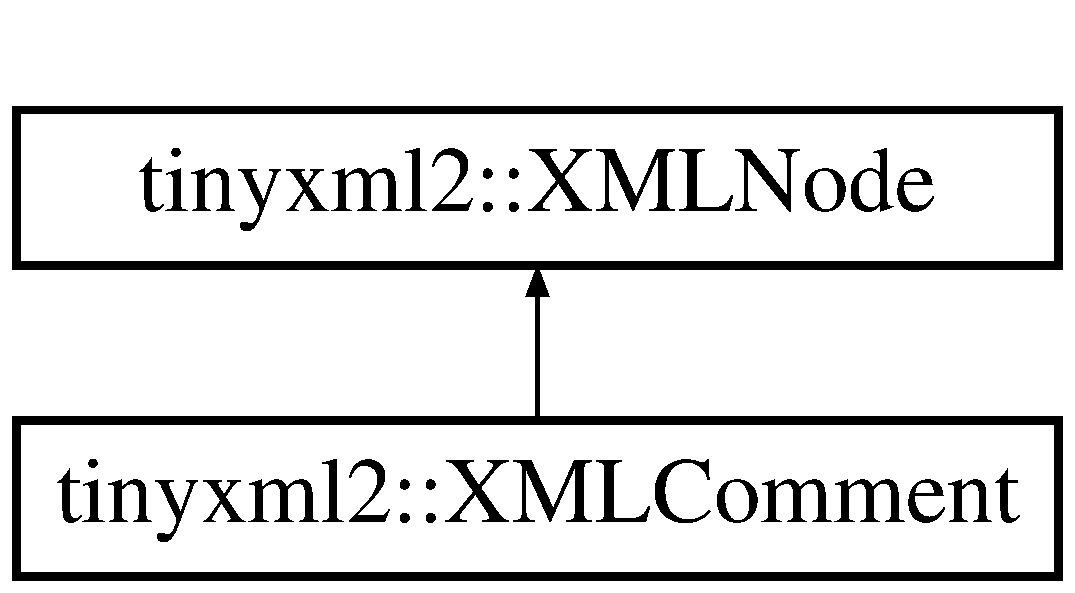
\includegraphics[height=2.000000cm]{classtinyxml2_1_1_x_m_l_comment}
\end{center}
\end{figure}
\subsection*{Public Member Functions}
\begin{DoxyCompactItemize}
\item 
virtual \hyperlink{classtinyxml2_1_1_x_m_l_comment}{X\+M\+L\+Comment} $\ast$ \hyperlink{classtinyxml2_1_1_x_m_l_comment_a8093e1dc8a34fa446d9dc3fde0e6c0ee}{To\+Comment} ()
\begin{DoxyCompactList}\small\item\em Safely cast to a Comment, or null. \end{DoxyCompactList}\item 
virtual const \hyperlink{classtinyxml2_1_1_x_m_l_comment}{X\+M\+L\+Comment} $\ast$ \hyperlink{classtinyxml2_1_1_x_m_l_comment_a422aabac22de7d9c9cad130897dd8b1c}{To\+Comment} () const 
\item 
virtual bool \hyperlink{classtinyxml2_1_1_x_m_l_comment_aa382b1be6a8b0650c16a2d88bb499335}{Accept} (\hyperlink{classtinyxml2_1_1_x_m_l_visitor}{X\+M\+L\+Visitor} $\ast$visitor) const 
\item 
char $\ast$ \hyperlink{classtinyxml2_1_1_x_m_l_comment_aa6ab35c3bb1c1840371dc32a2040c57f}{Parse\+Deep} (char $\ast$, \hyperlink{classtinyxml2_1_1_str_pair}{Str\+Pair} $\ast$end\+Tag)
\item 
virtual \hyperlink{classtinyxml2_1_1_x_m_l_node}{X\+M\+L\+Node} $\ast$ \hyperlink{classtinyxml2_1_1_x_m_l_comment_a90bb60193a691b484f5e1b487857016d}{Shallow\+Clone} (\hyperlink{classtinyxml2_1_1_x_m_l_document}{X\+M\+L\+Document} $\ast$document) const 
\item 
virtual bool \hyperlink{classtinyxml2_1_1_x_m_l_comment_a2d9f26757b0018fce933e74420cda22a}{Shallow\+Equal} (const \hyperlink{classtinyxml2_1_1_x_m_l_node}{X\+M\+L\+Node} $\ast$compare) const 
\end{DoxyCompactItemize}
\subsection*{Protected Member Functions}
\begin{DoxyCompactItemize}
\item 
\hyperlink{classtinyxml2_1_1_x_m_l_comment_ae6463adc3edd93a8e5a9b2b7e99cdf91}{X\+M\+L\+Comment} (\hyperlink{classtinyxml2_1_1_x_m_l_document}{X\+M\+L\+Document} $\ast$doc)
\item 
virtual \hyperlink{classtinyxml2_1_1_x_m_l_comment_ab592f69b47852455c1b32c5e31e453d0}{$\sim$\+X\+M\+L\+Comment} ()
\end{DoxyCompactItemize}
\subsection*{Friends}
\begin{DoxyCompactItemize}
\item 
class \hyperlink{classtinyxml2_1_1_x_m_l_comment_a4eee3bda60c60a30e4e8cd4ea91c4c6e}{X\+M\+L\+Document}
\end{DoxyCompactItemize}
\subsection*{Additional Inherited Members}


\subsection{Detailed Description}
An X\+M\+L Comment. 

\subsection{Constructor \& Destructor Documentation}
\hypertarget{classtinyxml2_1_1_x_m_l_comment_ae6463adc3edd93a8e5a9b2b7e99cdf91}{}\index{tinyxml2\+::\+X\+M\+L\+Comment@{tinyxml2\+::\+X\+M\+L\+Comment}!X\+M\+L\+Comment@{X\+M\+L\+Comment}}
\index{X\+M\+L\+Comment@{X\+M\+L\+Comment}!tinyxml2\+::\+X\+M\+L\+Comment@{tinyxml2\+::\+X\+M\+L\+Comment}}
\subsubsection[{X\+M\+L\+Comment}]{\setlength{\rightskip}{0pt plus 5cm}tinyxml2\+::\+X\+M\+L\+Comment\+::\+X\+M\+L\+Comment (
\begin{DoxyParamCaption}
\item[{{\bf X\+M\+L\+Document} $\ast$}]{doc}
\end{DoxyParamCaption}
)\hspace{0.3cm}{\ttfamily [protected]}}\label{classtinyxml2_1_1_x_m_l_comment_ae6463adc3edd93a8e5a9b2b7e99cdf91}
\hypertarget{classtinyxml2_1_1_x_m_l_comment_ab592f69b47852455c1b32c5e31e453d0}{}\index{tinyxml2\+::\+X\+M\+L\+Comment@{tinyxml2\+::\+X\+M\+L\+Comment}!````~X\+M\+L\+Comment@{$\sim$\+X\+M\+L\+Comment}}
\index{````~X\+M\+L\+Comment@{$\sim$\+X\+M\+L\+Comment}!tinyxml2\+::\+X\+M\+L\+Comment@{tinyxml2\+::\+X\+M\+L\+Comment}}
\subsubsection[{$\sim$\+X\+M\+L\+Comment}]{\setlength{\rightskip}{0pt plus 5cm}tinyxml2\+::\+X\+M\+L\+Comment\+::$\sim$\+X\+M\+L\+Comment (
\begin{DoxyParamCaption}
{}
\end{DoxyParamCaption}
)\hspace{0.3cm}{\ttfamily [protected]}, {\ttfamily [virtual]}}\label{classtinyxml2_1_1_x_m_l_comment_ab592f69b47852455c1b32c5e31e453d0}


\subsection{Member Function Documentation}
\hypertarget{classtinyxml2_1_1_x_m_l_comment_aa382b1be6a8b0650c16a2d88bb499335}{}\index{tinyxml2\+::\+X\+M\+L\+Comment@{tinyxml2\+::\+X\+M\+L\+Comment}!Accept@{Accept}}
\index{Accept@{Accept}!tinyxml2\+::\+X\+M\+L\+Comment@{tinyxml2\+::\+X\+M\+L\+Comment}}
\subsubsection[{Accept}]{\setlength{\rightskip}{0pt plus 5cm}bool tinyxml2\+::\+X\+M\+L\+Comment\+::\+Accept (
\begin{DoxyParamCaption}
\item[{{\bf X\+M\+L\+Visitor} $\ast$}]{visitor}
\end{DoxyParamCaption}
) const\hspace{0.3cm}{\ttfamily [virtual]}}\label{classtinyxml2_1_1_x_m_l_comment_aa382b1be6a8b0650c16a2d88bb499335}
Accept a hierarchical visit of the nodes in the Tiny\+X\+M\+L-\/2 D\+O\+M. Every node in the X\+M\+L tree will be conditionally visited and the host will be called back via the \hyperlink{classtinyxml2_1_1_x_m_l_visitor}{X\+M\+L\+Visitor} interface.

This is essentially a S\+A\+X interface for Tiny\+X\+M\+L-\/2. (Note however it doesn\textquotesingle{}t re-\/parse the X\+M\+L for the callbacks, so the performance of Tiny\+X\+M\+L-\/2 is unchanged by using this interface versus any other.)

The interface has been based on ideas from\+:


\begin{DoxyItemize}
\item \href{http://www.saxproject.org/}{\tt http\+://www.\+saxproject.\+org/}
\item \href{http://c2.com/cgi/wiki?HierarchicalVisitorPattern}{\tt http\+://c2.\+com/cgi/wiki?\+Hierarchical\+Visitor\+Pattern}
\end{DoxyItemize}

Which are both good references for \char`\"{}visiting\char`\"{}.

An example of using \hyperlink{classtinyxml2_1_1_x_m_l_comment_aa382b1be6a8b0650c16a2d88bb499335}{Accept()}\+: \begin{DoxyVerb}XMLPrinter printer;
tinyxmlDoc.Accept( &printer );
const char* xmlcstr = printer.CStr();
\end{DoxyVerb}
 

Implements \hyperlink{classtinyxml2_1_1_x_m_l_node_a81e66df0a44c67a7af17f3b77a152785}{tinyxml2\+::\+X\+M\+L\+Node}.

\hypertarget{classtinyxml2_1_1_x_m_l_comment_aa6ab35c3bb1c1840371dc32a2040c57f}{}\index{tinyxml2\+::\+X\+M\+L\+Comment@{tinyxml2\+::\+X\+M\+L\+Comment}!Parse\+Deep@{Parse\+Deep}}
\index{Parse\+Deep@{Parse\+Deep}!tinyxml2\+::\+X\+M\+L\+Comment@{tinyxml2\+::\+X\+M\+L\+Comment}}
\subsubsection[{Parse\+Deep}]{\setlength{\rightskip}{0pt plus 5cm}char $\ast$ tinyxml2\+::\+X\+M\+L\+Comment\+::\+Parse\+Deep (
\begin{DoxyParamCaption}
\item[{char $\ast$}]{p, }
\item[{{\bf Str\+Pair} $\ast$}]{end\+Tag}
\end{DoxyParamCaption}
)\hspace{0.3cm}{\ttfamily [virtual]}}\label{classtinyxml2_1_1_x_m_l_comment_aa6ab35c3bb1c1840371dc32a2040c57f}


Reimplemented from \hyperlink{classtinyxml2_1_1_x_m_l_node_a7610d0f603e8b603d2078521811a23c1}{tinyxml2\+::\+X\+M\+L\+Node}.

\hypertarget{classtinyxml2_1_1_x_m_l_comment_a90bb60193a691b484f5e1b487857016d}{}\index{tinyxml2\+::\+X\+M\+L\+Comment@{tinyxml2\+::\+X\+M\+L\+Comment}!Shallow\+Clone@{Shallow\+Clone}}
\index{Shallow\+Clone@{Shallow\+Clone}!tinyxml2\+::\+X\+M\+L\+Comment@{tinyxml2\+::\+X\+M\+L\+Comment}}
\subsubsection[{Shallow\+Clone}]{\setlength{\rightskip}{0pt plus 5cm}{\bf X\+M\+L\+Node} $\ast$ tinyxml2\+::\+X\+M\+L\+Comment\+::\+Shallow\+Clone (
\begin{DoxyParamCaption}
\item[{{\bf X\+M\+L\+Document} $\ast$}]{document}
\end{DoxyParamCaption}
) const\hspace{0.3cm}{\ttfamily [virtual]}}\label{classtinyxml2_1_1_x_m_l_comment_a90bb60193a691b484f5e1b487857016d}
Make a copy of this node, but not its children. You may pass in a Document pointer that will be the owner of the new Node. If the \textquotesingle{}document\textquotesingle{} is null, then the node returned will be allocated from the current Document. (this-\/$>$\hyperlink{classtinyxml2_1_1_x_m_l_node_af343d1ef0b45c0020e62d784d7e67a68}{Get\+Document()})

Note\+: if called on a \hyperlink{classtinyxml2_1_1_x_m_l_document}{X\+M\+L\+Document}, this will return null. 

Implements \hyperlink{classtinyxml2_1_1_x_m_l_node_a8402cbd3129d20e9e6024bbcc0531283}{tinyxml2\+::\+X\+M\+L\+Node}.

\hypertarget{classtinyxml2_1_1_x_m_l_comment_a2d9f26757b0018fce933e74420cda22a}{}\index{tinyxml2\+::\+X\+M\+L\+Comment@{tinyxml2\+::\+X\+M\+L\+Comment}!Shallow\+Equal@{Shallow\+Equal}}
\index{Shallow\+Equal@{Shallow\+Equal}!tinyxml2\+::\+X\+M\+L\+Comment@{tinyxml2\+::\+X\+M\+L\+Comment}}
\subsubsection[{Shallow\+Equal}]{\setlength{\rightskip}{0pt plus 5cm}bool tinyxml2\+::\+X\+M\+L\+Comment\+::\+Shallow\+Equal (
\begin{DoxyParamCaption}
\item[{const {\bf X\+M\+L\+Node} $\ast$}]{compare}
\end{DoxyParamCaption}
) const\hspace{0.3cm}{\ttfamily [virtual]}}\label{classtinyxml2_1_1_x_m_l_comment_a2d9f26757b0018fce933e74420cda22a}
Test if 2 nodes are the same, but don\textquotesingle{}t test children. The 2 nodes do not need to be in the same Document.

Note\+: if called on a \hyperlink{classtinyxml2_1_1_x_m_l_document}{X\+M\+L\+Document}, this will return false. 

Implements \hyperlink{classtinyxml2_1_1_x_m_l_node_a7ce18b751c3ea09eac292dca264f9226}{tinyxml2\+::\+X\+M\+L\+Node}.

\hypertarget{classtinyxml2_1_1_x_m_l_comment_a8093e1dc8a34fa446d9dc3fde0e6c0ee}{}\index{tinyxml2\+::\+X\+M\+L\+Comment@{tinyxml2\+::\+X\+M\+L\+Comment}!To\+Comment@{To\+Comment}}
\index{To\+Comment@{To\+Comment}!tinyxml2\+::\+X\+M\+L\+Comment@{tinyxml2\+::\+X\+M\+L\+Comment}}
\subsubsection[{To\+Comment}]{\setlength{\rightskip}{0pt plus 5cm}virtual {\bf X\+M\+L\+Comment}$\ast$ tinyxml2\+::\+X\+M\+L\+Comment\+::\+To\+Comment (
\begin{DoxyParamCaption}
{}
\end{DoxyParamCaption}
)\hspace{0.3cm}{\ttfamily [inline]}, {\ttfamily [virtual]}}\label{classtinyxml2_1_1_x_m_l_comment_a8093e1dc8a34fa446d9dc3fde0e6c0ee}


Safely cast to a Comment, or null. 



Reimplemented from \hyperlink{classtinyxml2_1_1_x_m_l_node_aff47671055aa99840a1c1ebd661e63e3}{tinyxml2\+::\+X\+M\+L\+Node}.

\hypertarget{classtinyxml2_1_1_x_m_l_comment_a422aabac22de7d9c9cad130897dd8b1c}{}\index{tinyxml2\+::\+X\+M\+L\+Comment@{tinyxml2\+::\+X\+M\+L\+Comment}!To\+Comment@{To\+Comment}}
\index{To\+Comment@{To\+Comment}!tinyxml2\+::\+X\+M\+L\+Comment@{tinyxml2\+::\+X\+M\+L\+Comment}}
\subsubsection[{To\+Comment}]{\setlength{\rightskip}{0pt plus 5cm}virtual const {\bf X\+M\+L\+Comment}$\ast$ tinyxml2\+::\+X\+M\+L\+Comment\+::\+To\+Comment (
\begin{DoxyParamCaption}
{}
\end{DoxyParamCaption}
) const\hspace{0.3cm}{\ttfamily [inline]}, {\ttfamily [virtual]}}\label{classtinyxml2_1_1_x_m_l_comment_a422aabac22de7d9c9cad130897dd8b1c}


Reimplemented from \hyperlink{classtinyxml2_1_1_x_m_l_node_a157ce3a00ea5ee5a85b7103138e85e8a}{tinyxml2\+::\+X\+M\+L\+Node}.



\subsection{Friends And Related Function Documentation}
\hypertarget{classtinyxml2_1_1_x_m_l_comment_a4eee3bda60c60a30e4e8cd4ea91c4c6e}{}\index{tinyxml2\+::\+X\+M\+L\+Comment@{tinyxml2\+::\+X\+M\+L\+Comment}!X\+M\+L\+Document@{X\+M\+L\+Document}}
\index{X\+M\+L\+Document@{X\+M\+L\+Document}!tinyxml2\+::\+X\+M\+L\+Comment@{tinyxml2\+::\+X\+M\+L\+Comment}}
\subsubsection[{X\+M\+L\+Document}]{\setlength{\rightskip}{0pt plus 5cm}friend class {\bf X\+M\+L\+Document}\hspace{0.3cm}{\ttfamily [friend]}}\label{classtinyxml2_1_1_x_m_l_comment_a4eee3bda60c60a30e4e8cd4ea91c4c6e}


The documentation for this class was generated from the following files\+:\begin{DoxyCompactItemize}
\item 
\hyperlink{tinyxml2_8h}{tinyxml2.\+h}\item 
\hyperlink{tinyxml2_8cpp}{tinyxml2.\+cpp}\end{DoxyCompactItemize}

\hypertarget{classtinyxml2_1_1_x_m_l_const_handle}{}\section{tinyxml2\+:\+:X\+M\+L\+Const\+Handle Class Reference}
\label{classtinyxml2_1_1_x_m_l_const_handle}\index{tinyxml2\+::\+X\+M\+L\+Const\+Handle@{tinyxml2\+::\+X\+M\+L\+Const\+Handle}}


{\ttfamily \#include $<$tinyxml2.\+h$>$}

\subsection*{Public Member Functions}
\begin{DoxyCompactItemize}
\item 
\hyperlink{classtinyxml2_1_1_x_m_l_const_handle_a098bda71fa11d7c74ccddab59d5dd534}{X\+M\+L\+Const\+Handle} (const \hyperlink{classtinyxml2_1_1_x_m_l_node}{X\+M\+L\+Node} $\ast$node)
\item 
\hyperlink{classtinyxml2_1_1_x_m_l_const_handle_a8420a0c4720637e0529e78c2e22f2b0b}{X\+M\+L\+Const\+Handle} (const \hyperlink{classtinyxml2_1_1_x_m_l_node}{X\+M\+L\+Node} \&node)
\item 
\hyperlink{classtinyxml2_1_1_x_m_l_const_handle_a639317ad315ff24f4ef0dc69312d7303}{X\+M\+L\+Const\+Handle} (const \hyperlink{classtinyxml2_1_1_x_m_l_const_handle}{X\+M\+L\+Const\+Handle} \&ref)
\item 
\hyperlink{classtinyxml2_1_1_x_m_l_const_handle}{X\+M\+L\+Const\+Handle} \& \hyperlink{classtinyxml2_1_1_x_m_l_const_handle_a2d74c91df1ff9aa5f9b57e3dceddbf94}{operator=} (const \hyperlink{classtinyxml2_1_1_x_m_l_const_handle}{X\+M\+L\+Const\+Handle} \&ref)
\item 
const \hyperlink{classtinyxml2_1_1_x_m_l_const_handle}{X\+M\+L\+Const\+Handle} \hyperlink{classtinyxml2_1_1_x_m_l_const_handle_a64c4ff7074effc1fd181d68d23f9d1e4}{First\+Child} () const 
\item 
const \hyperlink{classtinyxml2_1_1_x_m_l_const_handle}{X\+M\+L\+Const\+Handle} \hyperlink{classtinyxml2_1_1_x_m_l_const_handle_a5c197d0b57f8e560d93356a4a281469c}{First\+Child\+Element} (const char $\ast$value=0) const 
\item 
const \hyperlink{classtinyxml2_1_1_x_m_l_const_handle}{X\+M\+L\+Const\+Handle} \hyperlink{classtinyxml2_1_1_x_m_l_const_handle_afec9a68e7951193bc5a6e876d602f263}{Last\+Child} () const 
\item 
const \hyperlink{classtinyxml2_1_1_x_m_l_const_handle}{X\+M\+L\+Const\+Handle} \hyperlink{classtinyxml2_1_1_x_m_l_const_handle_a1c400e66dace6fdab4927adb21090059}{Last\+Child\+Element} (const char $\ast$\+\_\+value=0) const 
\item 
const \hyperlink{classtinyxml2_1_1_x_m_l_const_handle}{X\+M\+L\+Const\+Handle} \hyperlink{classtinyxml2_1_1_x_m_l_const_handle_a6917564e26b2c20ebdcb23c7940ad80a}{Previous\+Sibling} () const 
\item 
const \hyperlink{classtinyxml2_1_1_x_m_l_const_handle}{X\+M\+L\+Const\+Handle} \hyperlink{classtinyxml2_1_1_x_m_l_const_handle_acb2e1c5762eff9f6ed72d1a2dfc14271}{Previous\+Sibling\+Element} (const char $\ast$\+\_\+value=0) const 
\item 
const \hyperlink{classtinyxml2_1_1_x_m_l_const_handle}{X\+M\+L\+Const\+Handle} \hyperlink{classtinyxml2_1_1_x_m_l_const_handle_a596e248c8014d718f41658502a2e221b}{Next\+Sibling} () const 
\item 
const \hyperlink{classtinyxml2_1_1_x_m_l_const_handle}{X\+M\+L\+Const\+Handle} \hyperlink{classtinyxml2_1_1_x_m_l_const_handle_a3bbdd3d866c750473bd69a232704503b}{Next\+Sibling\+Element} (const char $\ast$\+\_\+value=0) const 
\item 
const \hyperlink{classtinyxml2_1_1_x_m_l_node}{X\+M\+L\+Node} $\ast$ \hyperlink{classtinyxml2_1_1_x_m_l_const_handle_a95d0256318c10c3f75fa5f8ffb3e4bc1}{To\+Node} () const 
\item 
const \hyperlink{classtinyxml2_1_1_x_m_l_element}{X\+M\+L\+Element} $\ast$ \hyperlink{classtinyxml2_1_1_x_m_l_const_handle_a5a48adefc2a5e70d4ce5b55692a0e2f9}{To\+Element} () const 
\item 
const \hyperlink{classtinyxml2_1_1_x_m_l_text}{X\+M\+L\+Text} $\ast$ \hyperlink{classtinyxml2_1_1_x_m_l_const_handle_ad86ca7dbb20d0495ae357fe7a866e0be}{To\+Text} () const 
\item 
const \hyperlink{classtinyxml2_1_1_x_m_l_unknown}{X\+M\+L\+Unknown} $\ast$ \hyperlink{classtinyxml2_1_1_x_m_l_const_handle_acb358a329e54fa204ed2d0b181566828}{To\+Unknown} () const 
\item 
const \hyperlink{classtinyxml2_1_1_x_m_l_declaration}{X\+M\+L\+Declaration} $\ast$ \hyperlink{classtinyxml2_1_1_x_m_l_const_handle_a5de0c175845bc30a6f9b3d88d8877eaf}{To\+Declaration} () const 
\end{DoxyCompactItemize}


\subsection{Detailed Description}
A variant of the \hyperlink{classtinyxml2_1_1_x_m_l_handle}{X\+M\+L\+Handle} class for working with const X\+M\+L\+Nodes and Documents. It is the same in all regards, except for the \textquotesingle{}const\textquotesingle{} qualifiers. See \hyperlink{classtinyxml2_1_1_x_m_l_handle}{X\+M\+L\+Handle} for A\+P\+I. 

\subsection{Constructor \& Destructor Documentation}
\hypertarget{classtinyxml2_1_1_x_m_l_const_handle_a098bda71fa11d7c74ccddab59d5dd534}{}\index{tinyxml2\+::\+X\+M\+L\+Const\+Handle@{tinyxml2\+::\+X\+M\+L\+Const\+Handle}!X\+M\+L\+Const\+Handle@{X\+M\+L\+Const\+Handle}}
\index{X\+M\+L\+Const\+Handle@{X\+M\+L\+Const\+Handle}!tinyxml2\+::\+X\+M\+L\+Const\+Handle@{tinyxml2\+::\+X\+M\+L\+Const\+Handle}}
\subsubsection[{X\+M\+L\+Const\+Handle}]{\setlength{\rightskip}{0pt plus 5cm}tinyxml2\+::\+X\+M\+L\+Const\+Handle\+::\+X\+M\+L\+Const\+Handle (
\begin{DoxyParamCaption}
\item[{const {\bf X\+M\+L\+Node} $\ast$}]{node}
\end{DoxyParamCaption}
)\hspace{0.3cm}{\ttfamily [inline]}}\label{classtinyxml2_1_1_x_m_l_const_handle_a098bda71fa11d7c74ccddab59d5dd534}
\hypertarget{classtinyxml2_1_1_x_m_l_const_handle_a8420a0c4720637e0529e78c2e22f2b0b}{}\index{tinyxml2\+::\+X\+M\+L\+Const\+Handle@{tinyxml2\+::\+X\+M\+L\+Const\+Handle}!X\+M\+L\+Const\+Handle@{X\+M\+L\+Const\+Handle}}
\index{X\+M\+L\+Const\+Handle@{X\+M\+L\+Const\+Handle}!tinyxml2\+::\+X\+M\+L\+Const\+Handle@{tinyxml2\+::\+X\+M\+L\+Const\+Handle}}
\subsubsection[{X\+M\+L\+Const\+Handle}]{\setlength{\rightskip}{0pt plus 5cm}tinyxml2\+::\+X\+M\+L\+Const\+Handle\+::\+X\+M\+L\+Const\+Handle (
\begin{DoxyParamCaption}
\item[{const {\bf X\+M\+L\+Node} \&}]{node}
\end{DoxyParamCaption}
)\hspace{0.3cm}{\ttfamily [inline]}}\label{classtinyxml2_1_1_x_m_l_const_handle_a8420a0c4720637e0529e78c2e22f2b0b}
\hypertarget{classtinyxml2_1_1_x_m_l_const_handle_a639317ad315ff24f4ef0dc69312d7303}{}\index{tinyxml2\+::\+X\+M\+L\+Const\+Handle@{tinyxml2\+::\+X\+M\+L\+Const\+Handle}!X\+M\+L\+Const\+Handle@{X\+M\+L\+Const\+Handle}}
\index{X\+M\+L\+Const\+Handle@{X\+M\+L\+Const\+Handle}!tinyxml2\+::\+X\+M\+L\+Const\+Handle@{tinyxml2\+::\+X\+M\+L\+Const\+Handle}}
\subsubsection[{X\+M\+L\+Const\+Handle}]{\setlength{\rightskip}{0pt plus 5cm}tinyxml2\+::\+X\+M\+L\+Const\+Handle\+::\+X\+M\+L\+Const\+Handle (
\begin{DoxyParamCaption}
\item[{const {\bf X\+M\+L\+Const\+Handle} \&}]{ref}
\end{DoxyParamCaption}
)\hspace{0.3cm}{\ttfamily [inline]}}\label{classtinyxml2_1_1_x_m_l_const_handle_a639317ad315ff24f4ef0dc69312d7303}


\subsection{Member Function Documentation}
\hypertarget{classtinyxml2_1_1_x_m_l_const_handle_a64c4ff7074effc1fd181d68d23f9d1e4}{}\index{tinyxml2\+::\+X\+M\+L\+Const\+Handle@{tinyxml2\+::\+X\+M\+L\+Const\+Handle}!First\+Child@{First\+Child}}
\index{First\+Child@{First\+Child}!tinyxml2\+::\+X\+M\+L\+Const\+Handle@{tinyxml2\+::\+X\+M\+L\+Const\+Handle}}
\subsubsection[{First\+Child}]{\setlength{\rightskip}{0pt plus 5cm}const {\bf X\+M\+L\+Const\+Handle} tinyxml2\+::\+X\+M\+L\+Const\+Handle\+::\+First\+Child (
\begin{DoxyParamCaption}
{}
\end{DoxyParamCaption}
) const\hspace{0.3cm}{\ttfamily [inline]}}\label{classtinyxml2_1_1_x_m_l_const_handle_a64c4ff7074effc1fd181d68d23f9d1e4}
\hypertarget{classtinyxml2_1_1_x_m_l_const_handle_a5c197d0b57f8e560d93356a4a281469c}{}\index{tinyxml2\+::\+X\+M\+L\+Const\+Handle@{tinyxml2\+::\+X\+M\+L\+Const\+Handle}!First\+Child\+Element@{First\+Child\+Element}}
\index{First\+Child\+Element@{First\+Child\+Element}!tinyxml2\+::\+X\+M\+L\+Const\+Handle@{tinyxml2\+::\+X\+M\+L\+Const\+Handle}}
\subsubsection[{First\+Child\+Element}]{\setlength{\rightskip}{0pt plus 5cm}const {\bf X\+M\+L\+Const\+Handle} tinyxml2\+::\+X\+M\+L\+Const\+Handle\+::\+First\+Child\+Element (
\begin{DoxyParamCaption}
\item[{const char $\ast$}]{value = {\ttfamily 0}}
\end{DoxyParamCaption}
) const\hspace{0.3cm}{\ttfamily [inline]}}\label{classtinyxml2_1_1_x_m_l_const_handle_a5c197d0b57f8e560d93356a4a281469c}
\hypertarget{classtinyxml2_1_1_x_m_l_const_handle_afec9a68e7951193bc5a6e876d602f263}{}\index{tinyxml2\+::\+X\+M\+L\+Const\+Handle@{tinyxml2\+::\+X\+M\+L\+Const\+Handle}!Last\+Child@{Last\+Child}}
\index{Last\+Child@{Last\+Child}!tinyxml2\+::\+X\+M\+L\+Const\+Handle@{tinyxml2\+::\+X\+M\+L\+Const\+Handle}}
\subsubsection[{Last\+Child}]{\setlength{\rightskip}{0pt plus 5cm}const {\bf X\+M\+L\+Const\+Handle} tinyxml2\+::\+X\+M\+L\+Const\+Handle\+::\+Last\+Child (
\begin{DoxyParamCaption}
{}
\end{DoxyParamCaption}
) const\hspace{0.3cm}{\ttfamily [inline]}}\label{classtinyxml2_1_1_x_m_l_const_handle_afec9a68e7951193bc5a6e876d602f263}
\hypertarget{classtinyxml2_1_1_x_m_l_const_handle_a1c400e66dace6fdab4927adb21090059}{}\index{tinyxml2\+::\+X\+M\+L\+Const\+Handle@{tinyxml2\+::\+X\+M\+L\+Const\+Handle}!Last\+Child\+Element@{Last\+Child\+Element}}
\index{Last\+Child\+Element@{Last\+Child\+Element}!tinyxml2\+::\+X\+M\+L\+Const\+Handle@{tinyxml2\+::\+X\+M\+L\+Const\+Handle}}
\subsubsection[{Last\+Child\+Element}]{\setlength{\rightskip}{0pt plus 5cm}const {\bf X\+M\+L\+Const\+Handle} tinyxml2\+::\+X\+M\+L\+Const\+Handle\+::\+Last\+Child\+Element (
\begin{DoxyParamCaption}
\item[{const char $\ast$}]{\+\_\+value = {\ttfamily 0}}
\end{DoxyParamCaption}
) const\hspace{0.3cm}{\ttfamily [inline]}}\label{classtinyxml2_1_1_x_m_l_const_handle_a1c400e66dace6fdab4927adb21090059}
\hypertarget{classtinyxml2_1_1_x_m_l_const_handle_a596e248c8014d718f41658502a2e221b}{}\index{tinyxml2\+::\+X\+M\+L\+Const\+Handle@{tinyxml2\+::\+X\+M\+L\+Const\+Handle}!Next\+Sibling@{Next\+Sibling}}
\index{Next\+Sibling@{Next\+Sibling}!tinyxml2\+::\+X\+M\+L\+Const\+Handle@{tinyxml2\+::\+X\+M\+L\+Const\+Handle}}
\subsubsection[{Next\+Sibling}]{\setlength{\rightskip}{0pt plus 5cm}const {\bf X\+M\+L\+Const\+Handle} tinyxml2\+::\+X\+M\+L\+Const\+Handle\+::\+Next\+Sibling (
\begin{DoxyParamCaption}
{}
\end{DoxyParamCaption}
) const\hspace{0.3cm}{\ttfamily [inline]}}\label{classtinyxml2_1_1_x_m_l_const_handle_a596e248c8014d718f41658502a2e221b}
\hypertarget{classtinyxml2_1_1_x_m_l_const_handle_a3bbdd3d866c750473bd69a232704503b}{}\index{tinyxml2\+::\+X\+M\+L\+Const\+Handle@{tinyxml2\+::\+X\+M\+L\+Const\+Handle}!Next\+Sibling\+Element@{Next\+Sibling\+Element}}
\index{Next\+Sibling\+Element@{Next\+Sibling\+Element}!tinyxml2\+::\+X\+M\+L\+Const\+Handle@{tinyxml2\+::\+X\+M\+L\+Const\+Handle}}
\subsubsection[{Next\+Sibling\+Element}]{\setlength{\rightskip}{0pt plus 5cm}const {\bf X\+M\+L\+Const\+Handle} tinyxml2\+::\+X\+M\+L\+Const\+Handle\+::\+Next\+Sibling\+Element (
\begin{DoxyParamCaption}
\item[{const char $\ast$}]{\+\_\+value = {\ttfamily 0}}
\end{DoxyParamCaption}
) const\hspace{0.3cm}{\ttfamily [inline]}}\label{classtinyxml2_1_1_x_m_l_const_handle_a3bbdd3d866c750473bd69a232704503b}
\hypertarget{classtinyxml2_1_1_x_m_l_const_handle_a2d74c91df1ff9aa5f9b57e3dceddbf94}{}\index{tinyxml2\+::\+X\+M\+L\+Const\+Handle@{tinyxml2\+::\+X\+M\+L\+Const\+Handle}!operator=@{operator=}}
\index{operator=@{operator=}!tinyxml2\+::\+X\+M\+L\+Const\+Handle@{tinyxml2\+::\+X\+M\+L\+Const\+Handle}}
\subsubsection[{operator=}]{\setlength{\rightskip}{0pt plus 5cm}{\bf X\+M\+L\+Const\+Handle}\& tinyxml2\+::\+X\+M\+L\+Const\+Handle\+::operator= (
\begin{DoxyParamCaption}
\item[{const {\bf X\+M\+L\+Const\+Handle} \&}]{ref}
\end{DoxyParamCaption}
)\hspace{0.3cm}{\ttfamily [inline]}}\label{classtinyxml2_1_1_x_m_l_const_handle_a2d74c91df1ff9aa5f9b57e3dceddbf94}
\hypertarget{classtinyxml2_1_1_x_m_l_const_handle_a6917564e26b2c20ebdcb23c7940ad80a}{}\index{tinyxml2\+::\+X\+M\+L\+Const\+Handle@{tinyxml2\+::\+X\+M\+L\+Const\+Handle}!Previous\+Sibling@{Previous\+Sibling}}
\index{Previous\+Sibling@{Previous\+Sibling}!tinyxml2\+::\+X\+M\+L\+Const\+Handle@{tinyxml2\+::\+X\+M\+L\+Const\+Handle}}
\subsubsection[{Previous\+Sibling}]{\setlength{\rightskip}{0pt plus 5cm}const {\bf X\+M\+L\+Const\+Handle} tinyxml2\+::\+X\+M\+L\+Const\+Handle\+::\+Previous\+Sibling (
\begin{DoxyParamCaption}
{}
\end{DoxyParamCaption}
) const\hspace{0.3cm}{\ttfamily [inline]}}\label{classtinyxml2_1_1_x_m_l_const_handle_a6917564e26b2c20ebdcb23c7940ad80a}
\hypertarget{classtinyxml2_1_1_x_m_l_const_handle_acb2e1c5762eff9f6ed72d1a2dfc14271}{}\index{tinyxml2\+::\+X\+M\+L\+Const\+Handle@{tinyxml2\+::\+X\+M\+L\+Const\+Handle}!Previous\+Sibling\+Element@{Previous\+Sibling\+Element}}
\index{Previous\+Sibling\+Element@{Previous\+Sibling\+Element}!tinyxml2\+::\+X\+M\+L\+Const\+Handle@{tinyxml2\+::\+X\+M\+L\+Const\+Handle}}
\subsubsection[{Previous\+Sibling\+Element}]{\setlength{\rightskip}{0pt plus 5cm}const {\bf X\+M\+L\+Const\+Handle} tinyxml2\+::\+X\+M\+L\+Const\+Handle\+::\+Previous\+Sibling\+Element (
\begin{DoxyParamCaption}
\item[{const char $\ast$}]{\+\_\+value = {\ttfamily 0}}
\end{DoxyParamCaption}
) const\hspace{0.3cm}{\ttfamily [inline]}}\label{classtinyxml2_1_1_x_m_l_const_handle_acb2e1c5762eff9f6ed72d1a2dfc14271}
\hypertarget{classtinyxml2_1_1_x_m_l_const_handle_a5de0c175845bc30a6f9b3d88d8877eaf}{}\index{tinyxml2\+::\+X\+M\+L\+Const\+Handle@{tinyxml2\+::\+X\+M\+L\+Const\+Handle}!To\+Declaration@{To\+Declaration}}
\index{To\+Declaration@{To\+Declaration}!tinyxml2\+::\+X\+M\+L\+Const\+Handle@{tinyxml2\+::\+X\+M\+L\+Const\+Handle}}
\subsubsection[{To\+Declaration}]{\setlength{\rightskip}{0pt plus 5cm}const {\bf X\+M\+L\+Declaration}$\ast$ tinyxml2\+::\+X\+M\+L\+Const\+Handle\+::\+To\+Declaration (
\begin{DoxyParamCaption}
{}
\end{DoxyParamCaption}
) const\hspace{0.3cm}{\ttfamily [inline]}}\label{classtinyxml2_1_1_x_m_l_const_handle_a5de0c175845bc30a6f9b3d88d8877eaf}
\hypertarget{classtinyxml2_1_1_x_m_l_const_handle_a5a48adefc2a5e70d4ce5b55692a0e2f9}{}\index{tinyxml2\+::\+X\+M\+L\+Const\+Handle@{tinyxml2\+::\+X\+M\+L\+Const\+Handle}!To\+Element@{To\+Element}}
\index{To\+Element@{To\+Element}!tinyxml2\+::\+X\+M\+L\+Const\+Handle@{tinyxml2\+::\+X\+M\+L\+Const\+Handle}}
\subsubsection[{To\+Element}]{\setlength{\rightskip}{0pt plus 5cm}const {\bf X\+M\+L\+Element}$\ast$ tinyxml2\+::\+X\+M\+L\+Const\+Handle\+::\+To\+Element (
\begin{DoxyParamCaption}
{}
\end{DoxyParamCaption}
) const\hspace{0.3cm}{\ttfamily [inline]}}\label{classtinyxml2_1_1_x_m_l_const_handle_a5a48adefc2a5e70d4ce5b55692a0e2f9}
\hypertarget{classtinyxml2_1_1_x_m_l_const_handle_a95d0256318c10c3f75fa5f8ffb3e4bc1}{}\index{tinyxml2\+::\+X\+M\+L\+Const\+Handle@{tinyxml2\+::\+X\+M\+L\+Const\+Handle}!To\+Node@{To\+Node}}
\index{To\+Node@{To\+Node}!tinyxml2\+::\+X\+M\+L\+Const\+Handle@{tinyxml2\+::\+X\+M\+L\+Const\+Handle}}
\subsubsection[{To\+Node}]{\setlength{\rightskip}{0pt plus 5cm}const {\bf X\+M\+L\+Node}$\ast$ tinyxml2\+::\+X\+M\+L\+Const\+Handle\+::\+To\+Node (
\begin{DoxyParamCaption}
{}
\end{DoxyParamCaption}
) const\hspace{0.3cm}{\ttfamily [inline]}}\label{classtinyxml2_1_1_x_m_l_const_handle_a95d0256318c10c3f75fa5f8ffb3e4bc1}
\hypertarget{classtinyxml2_1_1_x_m_l_const_handle_ad86ca7dbb20d0495ae357fe7a866e0be}{}\index{tinyxml2\+::\+X\+M\+L\+Const\+Handle@{tinyxml2\+::\+X\+M\+L\+Const\+Handle}!To\+Text@{To\+Text}}
\index{To\+Text@{To\+Text}!tinyxml2\+::\+X\+M\+L\+Const\+Handle@{tinyxml2\+::\+X\+M\+L\+Const\+Handle}}
\subsubsection[{To\+Text}]{\setlength{\rightskip}{0pt plus 5cm}const {\bf X\+M\+L\+Text}$\ast$ tinyxml2\+::\+X\+M\+L\+Const\+Handle\+::\+To\+Text (
\begin{DoxyParamCaption}
{}
\end{DoxyParamCaption}
) const\hspace{0.3cm}{\ttfamily [inline]}}\label{classtinyxml2_1_1_x_m_l_const_handle_ad86ca7dbb20d0495ae357fe7a866e0be}
\hypertarget{classtinyxml2_1_1_x_m_l_const_handle_acb358a329e54fa204ed2d0b181566828}{}\index{tinyxml2\+::\+X\+M\+L\+Const\+Handle@{tinyxml2\+::\+X\+M\+L\+Const\+Handle}!To\+Unknown@{To\+Unknown}}
\index{To\+Unknown@{To\+Unknown}!tinyxml2\+::\+X\+M\+L\+Const\+Handle@{tinyxml2\+::\+X\+M\+L\+Const\+Handle}}
\subsubsection[{To\+Unknown}]{\setlength{\rightskip}{0pt plus 5cm}const {\bf X\+M\+L\+Unknown}$\ast$ tinyxml2\+::\+X\+M\+L\+Const\+Handle\+::\+To\+Unknown (
\begin{DoxyParamCaption}
{}
\end{DoxyParamCaption}
) const\hspace{0.3cm}{\ttfamily [inline]}}\label{classtinyxml2_1_1_x_m_l_const_handle_acb358a329e54fa204ed2d0b181566828}


The documentation for this class was generated from the following file\+:\begin{DoxyCompactItemize}
\item 
\hyperlink{tinyxml2_8h}{tinyxml2.\+h}\end{DoxyCompactItemize}

\hypertarget{classtinyxml2_1_1_x_m_l_declaration}{}\section{tinyxml2\+:\+:X\+M\+L\+Declaration Class Reference}
\label{classtinyxml2_1_1_x_m_l_declaration}\index{tinyxml2\+::\+X\+M\+L\+Declaration@{tinyxml2\+::\+X\+M\+L\+Declaration}}


{\ttfamily \#include $<$tinyxml2.\+h$>$}

Inheritance diagram for tinyxml2\+:\+:X\+M\+L\+Declaration\+:\begin{figure}[H]
\begin{center}
\leavevmode
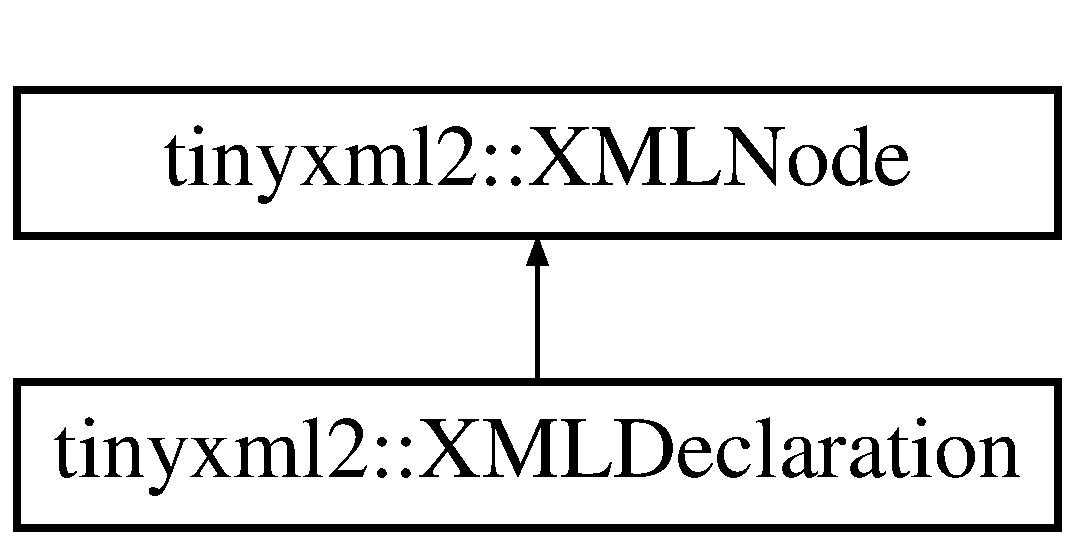
\includegraphics[height=2.000000cm]{classtinyxml2_1_1_x_m_l_declaration}
\end{center}
\end{figure}
\subsection*{Public Member Functions}
\begin{DoxyCompactItemize}
\item 
virtual \hyperlink{classtinyxml2_1_1_x_m_l_declaration}{X\+M\+L\+Declaration} $\ast$ \hyperlink{classtinyxml2_1_1_x_m_l_declaration_a159d8ac45865215e88059ea1e5b52fc5}{To\+Declaration} ()
\begin{DoxyCompactList}\small\item\em Safely cast to a Declaration, or null. \end{DoxyCompactList}\item 
virtual const \hyperlink{classtinyxml2_1_1_x_m_l_declaration}{X\+M\+L\+Declaration} $\ast$ \hyperlink{classtinyxml2_1_1_x_m_l_declaration_af724607a5fa810496fd6a21f5975a643}{To\+Declaration} () const 
\item 
virtual bool \hyperlink{classtinyxml2_1_1_x_m_l_declaration_a953a7359cc312d15218eb5843a4ca108}{Accept} (\hyperlink{classtinyxml2_1_1_x_m_l_visitor}{X\+M\+L\+Visitor} $\ast$visitor) const 
\item 
char $\ast$ \hyperlink{classtinyxml2_1_1_x_m_l_declaration_a19e33e0a9f9500f449261558c36f9a44}{Parse\+Deep} (char $\ast$, \hyperlink{classtinyxml2_1_1_str_pair}{Str\+Pair} $\ast$end\+Tag)
\item 
virtual \hyperlink{classtinyxml2_1_1_x_m_l_node}{X\+M\+L\+Node} $\ast$ \hyperlink{classtinyxml2_1_1_x_m_l_declaration_a39458732ee6796cfc85dd35d3c488e0b}{Shallow\+Clone} (\hyperlink{classtinyxml2_1_1_x_m_l_document}{X\+M\+L\+Document} $\ast$document) const 
\item 
virtual bool \hyperlink{classtinyxml2_1_1_x_m_l_declaration_ace0d2d9bc1b63278bd5e984ebe0c7bd0}{Shallow\+Equal} (const \hyperlink{classtinyxml2_1_1_x_m_l_node}{X\+M\+L\+Node} $\ast$compare) const 
\end{DoxyCompactItemize}
\subsection*{Protected Member Functions}
\begin{DoxyCompactItemize}
\item 
\hyperlink{classtinyxml2_1_1_x_m_l_declaration_aef9586f2ce5df5feba74dde49a242b06}{X\+M\+L\+Declaration} (\hyperlink{classtinyxml2_1_1_x_m_l_document}{X\+M\+L\+Document} $\ast$doc)
\item 
virtual \hyperlink{classtinyxml2_1_1_x_m_l_declaration_ab93d5bf4f5d58b4144963cf739cf6dcc}{$\sim$\+X\+M\+L\+Declaration} ()
\end{DoxyCompactItemize}
\subsection*{Friends}
\begin{DoxyCompactItemize}
\item 
class \hyperlink{classtinyxml2_1_1_x_m_l_declaration_a4eee3bda60c60a30e4e8cd4ea91c4c6e}{X\+M\+L\+Document}
\end{DoxyCompactItemize}
\subsection*{Additional Inherited Members}


\subsection{Detailed Description}
In correct X\+M\+L the declaration is the first entry in the file. \begin{DoxyVerb}    <?xml version="1.0" standalone="yes"?>
\end{DoxyVerb}


Tiny\+X\+M\+L-\/2 will happily read or write files without a declaration, however.

The text of the declaration isn\textquotesingle{}t interpreted. It is parsed and written as a string. 

\subsection{Constructor \& Destructor Documentation}
\hypertarget{classtinyxml2_1_1_x_m_l_declaration_aef9586f2ce5df5feba74dde49a242b06}{}\index{tinyxml2\+::\+X\+M\+L\+Declaration@{tinyxml2\+::\+X\+M\+L\+Declaration}!X\+M\+L\+Declaration@{X\+M\+L\+Declaration}}
\index{X\+M\+L\+Declaration@{X\+M\+L\+Declaration}!tinyxml2\+::\+X\+M\+L\+Declaration@{tinyxml2\+::\+X\+M\+L\+Declaration}}
\subsubsection[{X\+M\+L\+Declaration}]{\setlength{\rightskip}{0pt plus 5cm}tinyxml2\+::\+X\+M\+L\+Declaration\+::\+X\+M\+L\+Declaration (
\begin{DoxyParamCaption}
\item[{{\bf X\+M\+L\+Document} $\ast$}]{doc}
\end{DoxyParamCaption}
)\hspace{0.3cm}{\ttfamily [protected]}}\label{classtinyxml2_1_1_x_m_l_declaration_aef9586f2ce5df5feba74dde49a242b06}
\hypertarget{classtinyxml2_1_1_x_m_l_declaration_ab93d5bf4f5d58b4144963cf739cf6dcc}{}\index{tinyxml2\+::\+X\+M\+L\+Declaration@{tinyxml2\+::\+X\+M\+L\+Declaration}!````~X\+M\+L\+Declaration@{$\sim$\+X\+M\+L\+Declaration}}
\index{````~X\+M\+L\+Declaration@{$\sim$\+X\+M\+L\+Declaration}!tinyxml2\+::\+X\+M\+L\+Declaration@{tinyxml2\+::\+X\+M\+L\+Declaration}}
\subsubsection[{$\sim$\+X\+M\+L\+Declaration}]{\setlength{\rightskip}{0pt plus 5cm}tinyxml2\+::\+X\+M\+L\+Declaration\+::$\sim$\+X\+M\+L\+Declaration (
\begin{DoxyParamCaption}
{}
\end{DoxyParamCaption}
)\hspace{0.3cm}{\ttfamily [protected]}, {\ttfamily [virtual]}}\label{classtinyxml2_1_1_x_m_l_declaration_ab93d5bf4f5d58b4144963cf739cf6dcc}


\subsection{Member Function Documentation}
\hypertarget{classtinyxml2_1_1_x_m_l_declaration_a953a7359cc312d15218eb5843a4ca108}{}\index{tinyxml2\+::\+X\+M\+L\+Declaration@{tinyxml2\+::\+X\+M\+L\+Declaration}!Accept@{Accept}}
\index{Accept@{Accept}!tinyxml2\+::\+X\+M\+L\+Declaration@{tinyxml2\+::\+X\+M\+L\+Declaration}}
\subsubsection[{Accept}]{\setlength{\rightskip}{0pt plus 5cm}bool tinyxml2\+::\+X\+M\+L\+Declaration\+::\+Accept (
\begin{DoxyParamCaption}
\item[{{\bf X\+M\+L\+Visitor} $\ast$}]{visitor}
\end{DoxyParamCaption}
) const\hspace{0.3cm}{\ttfamily [virtual]}}\label{classtinyxml2_1_1_x_m_l_declaration_a953a7359cc312d15218eb5843a4ca108}
Accept a hierarchical visit of the nodes in the Tiny\+X\+M\+L-\/2 D\+O\+M. Every node in the X\+M\+L tree will be conditionally visited and the host will be called back via the \hyperlink{classtinyxml2_1_1_x_m_l_visitor}{X\+M\+L\+Visitor} interface.

This is essentially a S\+A\+X interface for Tiny\+X\+M\+L-\/2. (Note however it doesn\textquotesingle{}t re-\/parse the X\+M\+L for the callbacks, so the performance of Tiny\+X\+M\+L-\/2 is unchanged by using this interface versus any other.)

The interface has been based on ideas from\+:


\begin{DoxyItemize}
\item \href{http://www.saxproject.org/}{\tt http\+://www.\+saxproject.\+org/}
\item \href{http://c2.com/cgi/wiki?HierarchicalVisitorPattern}{\tt http\+://c2.\+com/cgi/wiki?\+Hierarchical\+Visitor\+Pattern}
\end{DoxyItemize}

Which are both good references for \char`\"{}visiting\char`\"{}.

An example of using \hyperlink{classtinyxml2_1_1_x_m_l_declaration_a953a7359cc312d15218eb5843a4ca108}{Accept()}\+: \begin{DoxyVerb}XMLPrinter printer;
tinyxmlDoc.Accept( &printer );
const char* xmlcstr = printer.CStr();
\end{DoxyVerb}
 

Implements \hyperlink{classtinyxml2_1_1_x_m_l_node_a81e66df0a44c67a7af17f3b77a152785}{tinyxml2\+::\+X\+M\+L\+Node}.

\hypertarget{classtinyxml2_1_1_x_m_l_declaration_a19e33e0a9f9500f449261558c36f9a44}{}\index{tinyxml2\+::\+X\+M\+L\+Declaration@{tinyxml2\+::\+X\+M\+L\+Declaration}!Parse\+Deep@{Parse\+Deep}}
\index{Parse\+Deep@{Parse\+Deep}!tinyxml2\+::\+X\+M\+L\+Declaration@{tinyxml2\+::\+X\+M\+L\+Declaration}}
\subsubsection[{Parse\+Deep}]{\setlength{\rightskip}{0pt plus 5cm}char $\ast$ tinyxml2\+::\+X\+M\+L\+Declaration\+::\+Parse\+Deep (
\begin{DoxyParamCaption}
\item[{char $\ast$}]{p, }
\item[{{\bf Str\+Pair} $\ast$}]{end\+Tag}
\end{DoxyParamCaption}
)\hspace{0.3cm}{\ttfamily [virtual]}}\label{classtinyxml2_1_1_x_m_l_declaration_a19e33e0a9f9500f449261558c36f9a44}


Reimplemented from \hyperlink{classtinyxml2_1_1_x_m_l_node_a7610d0f603e8b603d2078521811a23c1}{tinyxml2\+::\+X\+M\+L\+Node}.

\hypertarget{classtinyxml2_1_1_x_m_l_declaration_a39458732ee6796cfc85dd35d3c488e0b}{}\index{tinyxml2\+::\+X\+M\+L\+Declaration@{tinyxml2\+::\+X\+M\+L\+Declaration}!Shallow\+Clone@{Shallow\+Clone}}
\index{Shallow\+Clone@{Shallow\+Clone}!tinyxml2\+::\+X\+M\+L\+Declaration@{tinyxml2\+::\+X\+M\+L\+Declaration}}
\subsubsection[{Shallow\+Clone}]{\setlength{\rightskip}{0pt plus 5cm}{\bf X\+M\+L\+Node} $\ast$ tinyxml2\+::\+X\+M\+L\+Declaration\+::\+Shallow\+Clone (
\begin{DoxyParamCaption}
\item[{{\bf X\+M\+L\+Document} $\ast$}]{document}
\end{DoxyParamCaption}
) const\hspace{0.3cm}{\ttfamily [virtual]}}\label{classtinyxml2_1_1_x_m_l_declaration_a39458732ee6796cfc85dd35d3c488e0b}
Make a copy of this node, but not its children. You may pass in a Document pointer that will be the owner of the new Node. If the \textquotesingle{}document\textquotesingle{} is null, then the node returned will be allocated from the current Document. (this-\/$>$\hyperlink{classtinyxml2_1_1_x_m_l_node_af343d1ef0b45c0020e62d784d7e67a68}{Get\+Document()})

Note\+: if called on a \hyperlink{classtinyxml2_1_1_x_m_l_document}{X\+M\+L\+Document}, this will return null. 

Implements \hyperlink{classtinyxml2_1_1_x_m_l_node_a8402cbd3129d20e9e6024bbcc0531283}{tinyxml2\+::\+X\+M\+L\+Node}.

\hypertarget{classtinyxml2_1_1_x_m_l_declaration_ace0d2d9bc1b63278bd5e984ebe0c7bd0}{}\index{tinyxml2\+::\+X\+M\+L\+Declaration@{tinyxml2\+::\+X\+M\+L\+Declaration}!Shallow\+Equal@{Shallow\+Equal}}
\index{Shallow\+Equal@{Shallow\+Equal}!tinyxml2\+::\+X\+M\+L\+Declaration@{tinyxml2\+::\+X\+M\+L\+Declaration}}
\subsubsection[{Shallow\+Equal}]{\setlength{\rightskip}{0pt plus 5cm}bool tinyxml2\+::\+X\+M\+L\+Declaration\+::\+Shallow\+Equal (
\begin{DoxyParamCaption}
\item[{const {\bf X\+M\+L\+Node} $\ast$}]{compare}
\end{DoxyParamCaption}
) const\hspace{0.3cm}{\ttfamily [virtual]}}\label{classtinyxml2_1_1_x_m_l_declaration_ace0d2d9bc1b63278bd5e984ebe0c7bd0}
Test if 2 nodes are the same, but don\textquotesingle{}t test children. The 2 nodes do not need to be in the same Document.

Note\+: if called on a \hyperlink{classtinyxml2_1_1_x_m_l_document}{X\+M\+L\+Document}, this will return false. 

Implements \hyperlink{classtinyxml2_1_1_x_m_l_node_a7ce18b751c3ea09eac292dca264f9226}{tinyxml2\+::\+X\+M\+L\+Node}.

\hypertarget{classtinyxml2_1_1_x_m_l_declaration_a159d8ac45865215e88059ea1e5b52fc5}{}\index{tinyxml2\+::\+X\+M\+L\+Declaration@{tinyxml2\+::\+X\+M\+L\+Declaration}!To\+Declaration@{To\+Declaration}}
\index{To\+Declaration@{To\+Declaration}!tinyxml2\+::\+X\+M\+L\+Declaration@{tinyxml2\+::\+X\+M\+L\+Declaration}}
\subsubsection[{To\+Declaration}]{\setlength{\rightskip}{0pt plus 5cm}virtual {\bf X\+M\+L\+Declaration}$\ast$ tinyxml2\+::\+X\+M\+L\+Declaration\+::\+To\+Declaration (
\begin{DoxyParamCaption}
{}
\end{DoxyParamCaption}
)\hspace{0.3cm}{\ttfamily [inline]}, {\ttfamily [virtual]}}\label{classtinyxml2_1_1_x_m_l_declaration_a159d8ac45865215e88059ea1e5b52fc5}


Safely cast to a Declaration, or null. 



Reimplemented from \hyperlink{classtinyxml2_1_1_x_m_l_node_a174fd4c22c010b58138c1b84a0dfbd51}{tinyxml2\+::\+X\+M\+L\+Node}.

\hypertarget{classtinyxml2_1_1_x_m_l_declaration_af724607a5fa810496fd6a21f5975a643}{}\index{tinyxml2\+::\+X\+M\+L\+Declaration@{tinyxml2\+::\+X\+M\+L\+Declaration}!To\+Declaration@{To\+Declaration}}
\index{To\+Declaration@{To\+Declaration}!tinyxml2\+::\+X\+M\+L\+Declaration@{tinyxml2\+::\+X\+M\+L\+Declaration}}
\subsubsection[{To\+Declaration}]{\setlength{\rightskip}{0pt plus 5cm}virtual const {\bf X\+M\+L\+Declaration}$\ast$ tinyxml2\+::\+X\+M\+L\+Declaration\+::\+To\+Declaration (
\begin{DoxyParamCaption}
{}
\end{DoxyParamCaption}
) const\hspace{0.3cm}{\ttfamily [inline]}, {\ttfamily [virtual]}}\label{classtinyxml2_1_1_x_m_l_declaration_af724607a5fa810496fd6a21f5975a643}


Reimplemented from \hyperlink{classtinyxml2_1_1_x_m_l_node_aedae0bbb58d533a4b8a61042388b49e5}{tinyxml2\+::\+X\+M\+L\+Node}.



\subsection{Friends And Related Function Documentation}
\hypertarget{classtinyxml2_1_1_x_m_l_declaration_a4eee3bda60c60a30e4e8cd4ea91c4c6e}{}\index{tinyxml2\+::\+X\+M\+L\+Declaration@{tinyxml2\+::\+X\+M\+L\+Declaration}!X\+M\+L\+Document@{X\+M\+L\+Document}}
\index{X\+M\+L\+Document@{X\+M\+L\+Document}!tinyxml2\+::\+X\+M\+L\+Declaration@{tinyxml2\+::\+X\+M\+L\+Declaration}}
\subsubsection[{X\+M\+L\+Document}]{\setlength{\rightskip}{0pt plus 5cm}friend class {\bf X\+M\+L\+Document}\hspace{0.3cm}{\ttfamily [friend]}}\label{classtinyxml2_1_1_x_m_l_declaration_a4eee3bda60c60a30e4e8cd4ea91c4c6e}


The documentation for this class was generated from the following files\+:\begin{DoxyCompactItemize}
\item 
\hyperlink{tinyxml2_8h}{tinyxml2.\+h}\item 
\hyperlink{tinyxml2_8cpp}{tinyxml2.\+cpp}\end{DoxyCompactItemize}

\hypertarget{classtinyxml2_1_1_x_m_l_document}{}\section{tinyxml2\+:\+:X\+M\+L\+Document Class Reference}
\label{classtinyxml2_1_1_x_m_l_document}\index{tinyxml2\+::\+X\+M\+L\+Document@{tinyxml2\+::\+X\+M\+L\+Document}}


{\ttfamily \#include $<$tinyxml2.\+h$>$}

Inheritance diagram for tinyxml2\+:\+:X\+M\+L\+Document\+:\begin{figure}[H]
\begin{center}
\leavevmode
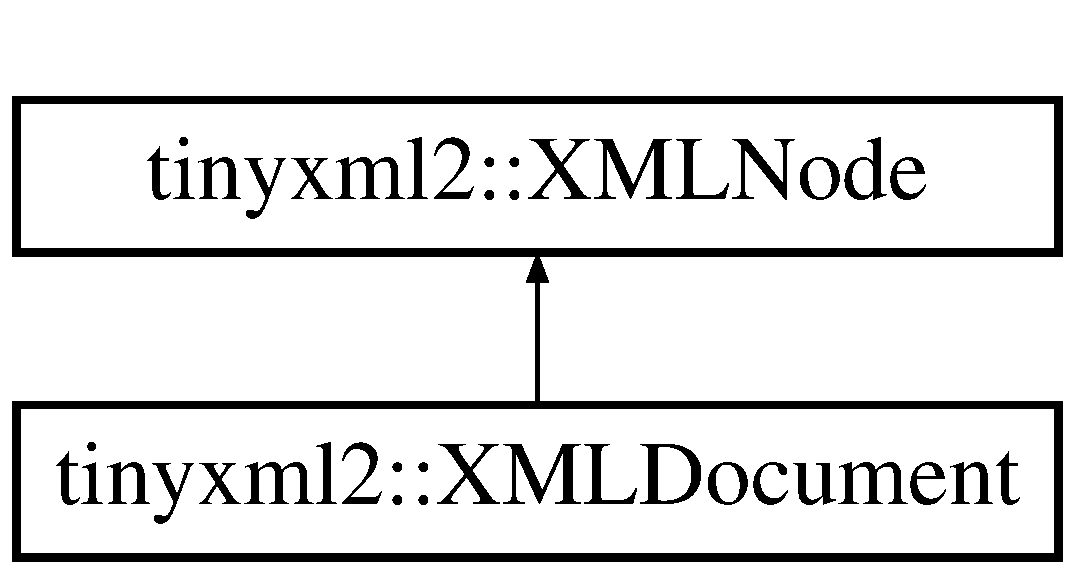
\includegraphics[height=2.000000cm]{classtinyxml2_1_1_x_m_l_document}
\end{center}
\end{figure}
\subsection*{Public Member Functions}
\begin{DoxyCompactItemize}
\item 
\hyperlink{classtinyxml2_1_1_x_m_l_document_af1574f76ebb619f25ef3f09eb2ba5188}{X\+M\+L\+Document} (bool process\+Entities=true, \hyperlink{namespacetinyxml2_a7f91d00f77360f850fd5da0861e27dd5}{Whitespace}=\hyperlink{namespacetinyxml2_a7f91d00f77360f850fd5da0861e27dd5a751769aa625fe5fe5286e9779edec56a}{P\+R\+E\+S\+E\+R\+V\+E\+\_\+\+W\+H\+I\+T\+E\+S\+P\+A\+C\+E})
\begin{DoxyCompactList}\small\item\em constructor \end{DoxyCompactList}\item 
\hyperlink{classtinyxml2_1_1_x_m_l_document_af37c47d8e2ba4b2fc81b21a77a32579b}{$\sim$\+X\+M\+L\+Document} ()
\item 
virtual \hyperlink{classtinyxml2_1_1_x_m_l_document}{X\+M\+L\+Document} $\ast$ \hyperlink{classtinyxml2_1_1_x_m_l_document_a3e185f880882bd978367bb55937735ec}{To\+Document} ()
\begin{DoxyCompactList}\small\item\em Safely cast to a Document, or null. \end{DoxyCompactList}\item 
virtual const \hyperlink{classtinyxml2_1_1_x_m_l_document}{X\+M\+L\+Document} $\ast$ \hyperlink{classtinyxml2_1_1_x_m_l_document_a15eb1a62afa18c66808031da647d1129}{To\+Document} () const 
\item 
\hyperlink{namespacetinyxml2_a1fbf88509c3ac88c09117b1947414e08}{X\+M\+L\+Error} \hyperlink{classtinyxml2_1_1_x_m_l_document_a1819bd34f540a7304c105a6232d25a1f}{Parse} (const char $\ast$xml, size\+\_\+t n\+Bytes=(size\+\_\+t)(-\/1))
\item 
\hyperlink{namespacetinyxml2_a1fbf88509c3ac88c09117b1947414e08}{X\+M\+L\+Error} \hyperlink{classtinyxml2_1_1_x_m_l_document_a2ebd4647a8af5fc6831b294ac26a150a}{Load\+File} (const char $\ast$filename)
\item 
\hyperlink{namespacetinyxml2_a1fbf88509c3ac88c09117b1947414e08}{X\+M\+L\+Error} \hyperlink{classtinyxml2_1_1_x_m_l_document_a5f1d330fad44c52f3d265338dd2a6dc2}{Load\+File} (F\+I\+L\+E $\ast$)
\item 
\hyperlink{namespacetinyxml2_a1fbf88509c3ac88c09117b1947414e08}{X\+M\+L\+Error} \hyperlink{classtinyxml2_1_1_x_m_l_document_a73ac416b4a2aa0952e841220eb3da18f}{Save\+File} (const char $\ast$filename, bool compact=false)
\item 
\hyperlink{namespacetinyxml2_a1fbf88509c3ac88c09117b1947414e08}{X\+M\+L\+Error} \hyperlink{classtinyxml2_1_1_x_m_l_document_a8b95779479a0035acc67b3a61dfe1b74}{Save\+File} (F\+I\+L\+E $\ast$fp, bool compact=false)
\item 
bool \hyperlink{classtinyxml2_1_1_x_m_l_document_adfcff7d0599cd520e9fcbb8891e1b678}{Process\+Entities} () const 
\item 
\hyperlink{namespacetinyxml2_a7f91d00f77360f850fd5da0861e27dd5}{Whitespace} \hyperlink{classtinyxml2_1_1_x_m_l_document_a94b3ea2f77c9ac831723984df5a02d01}{Whitespace\+Mode} () const 
\item 
bool \hyperlink{classtinyxml2_1_1_x_m_l_document_a530649e9de7e5aa8df9c37f66197fcb6}{Has\+B\+O\+M} () const 
\item 
void \hyperlink{classtinyxml2_1_1_x_m_l_document_a14419b698f7c4b140df4e80f3f0c93b0}{Set\+B\+O\+M} (bool use\+B\+O\+M)
\item 
\hyperlink{classtinyxml2_1_1_x_m_l_element}{X\+M\+L\+Element} $\ast$ \hyperlink{classtinyxml2_1_1_x_m_l_document_ad2b70320d3c2a071c2f36928edff3e1c}{Root\+Element} ()
\item 
const \hyperlink{classtinyxml2_1_1_x_m_l_element}{X\+M\+L\+Element} $\ast$ \hyperlink{classtinyxml2_1_1_x_m_l_document_a23a25b573d2adf3ee6075636c2a31c73}{Root\+Element} () const 
\item 
void \hyperlink{classtinyxml2_1_1_x_m_l_document_a686ea28672c0e0c60383ec28148c1ac0}{Print} (\hyperlink{classtinyxml2_1_1_x_m_l_printer}{X\+M\+L\+Printer} $\ast$streamer=0) const 
\item 
virtual bool \hyperlink{classtinyxml2_1_1_x_m_l_document_aa08503d24898bf9992ae5e5fb8b0cf87}{Accept} (\hyperlink{classtinyxml2_1_1_x_m_l_visitor}{X\+M\+L\+Visitor} $\ast$visitor) const 
\item 
\hyperlink{classtinyxml2_1_1_x_m_l_element}{X\+M\+L\+Element} $\ast$ \hyperlink{classtinyxml2_1_1_x_m_l_document_a3c335a700a43d7c363a393142a23f234}{New\+Element} (const char $\ast$name)
\item 
\hyperlink{classtinyxml2_1_1_x_m_l_comment}{X\+M\+L\+Comment} $\ast$ \hyperlink{classtinyxml2_1_1_x_m_l_document_a386df0befd06aadb5e0cd21381aa955a}{New\+Comment} (const char $\ast$comment)
\item 
\hyperlink{classtinyxml2_1_1_x_m_l_text}{X\+M\+L\+Text} $\ast$ \hyperlink{classtinyxml2_1_1_x_m_l_document_acece5de77a0819f2341b08c1e1ed9987}{New\+Text} (const char $\ast$text)
\item 
\hyperlink{classtinyxml2_1_1_x_m_l_declaration}{X\+M\+L\+Declaration} $\ast$ \hyperlink{classtinyxml2_1_1_x_m_l_document_ae519030c0262fa2daff8993681990e16}{New\+Declaration} (const char $\ast$text=0)
\item 
\hyperlink{classtinyxml2_1_1_x_m_l_unknown}{X\+M\+L\+Unknown} $\ast$ \hyperlink{classtinyxml2_1_1_x_m_l_document_a4954f502c5fd7f49de54c3c0c99bb73d}{New\+Unknown} (const char $\ast$text)
\item 
void \hyperlink{classtinyxml2_1_1_x_m_l_document_ac1d6e2c7fcc1a660624ac4f68e96380d}{Delete\+Node} (\hyperlink{classtinyxml2_1_1_x_m_l_node}{X\+M\+L\+Node} $\ast$node)
\item 
void \hyperlink{classtinyxml2_1_1_x_m_l_document_ae38d194e47336e4c96677ac77e2ac5d4}{Set\+Error} (\hyperlink{namespacetinyxml2_a1fbf88509c3ac88c09117b1947414e08}{X\+M\+L\+Error} error, const char $\ast$str1, const char $\ast$str2)
\item 
bool \hyperlink{classtinyxml2_1_1_x_m_l_document_abf0f9ac4c3aa5698a785937f71f7a69f}{Error} () const 
\begin{DoxyCompactList}\small\item\em Return true if there was an error parsing the document. \end{DoxyCompactList}\item 
\hyperlink{namespacetinyxml2_a1fbf88509c3ac88c09117b1947414e08}{X\+M\+L\+Error} \hyperlink{classtinyxml2_1_1_x_m_l_document_a34903418c9e83f27945c2c533839e350}{Error\+I\+D} () const 
\begin{DoxyCompactList}\small\item\em Return the error\+I\+D. \end{DoxyCompactList}\item 
const char $\ast$ \hyperlink{classtinyxml2_1_1_x_m_l_document_a7ff8b68f87042d535841b0afd2c82161}{Error\+Name} () const 
\item 
const char $\ast$ \hyperlink{classtinyxml2_1_1_x_m_l_document_a016ccebecee36fe92084b5dfee6cc072}{Get\+Error\+Str1} () const 
\begin{DoxyCompactList}\small\item\em Return a possibly helpful diagnostic location or string. \end{DoxyCompactList}\item 
const char $\ast$ \hyperlink{classtinyxml2_1_1_x_m_l_document_a88f6b44bd019033bda28abd31fe257b2}{Get\+Error\+Str2} () const 
\begin{DoxyCompactList}\small\item\em Return a possibly helpful secondary diagnostic location or string. \end{DoxyCompactList}\item 
void \hyperlink{classtinyxml2_1_1_x_m_l_document_a7545cc9a9a67eee9307c001aa316a388}{Print\+Error} () const 
\begin{DoxyCompactList}\small\item\em If there is an error, print it to stdout. \end{DoxyCompactList}\item 
void \hyperlink{classtinyxml2_1_1_x_m_l_document_a65656b0b2cbc822708eb351504178aaf}{Clear} ()
\begin{DoxyCompactList}\small\item\em Clear the document, resetting it to the initial state. \end{DoxyCompactList}\item 
char $\ast$ \hyperlink{classtinyxml2_1_1_x_m_l_document_a25827d1bec509ad566a107e5853ed040}{Identify} (char $\ast$p, \hyperlink{classtinyxml2_1_1_x_m_l_node}{X\+M\+L\+Node} $\ast$$\ast$node)
\item 
virtual \hyperlink{classtinyxml2_1_1_x_m_l_node}{X\+M\+L\+Node} $\ast$ \hyperlink{classtinyxml2_1_1_x_m_l_document_a57c8511ed9f83aa3e20909a3db3f83d0}{Shallow\+Clone} (\hyperlink{classtinyxml2_1_1_x_m_l_document}{X\+M\+L\+Document} $\ast$) const 
\item 
virtual bool \hyperlink{classtinyxml2_1_1_x_m_l_document_a12eac66c6e45d074d5cc47319868cd66}{Shallow\+Equal} (const \hyperlink{classtinyxml2_1_1_x_m_l_node}{X\+M\+L\+Node} $\ast$) const 
\end{DoxyCompactItemize}
\subsection*{Friends}
\begin{DoxyCompactItemize}
\item 
class \hyperlink{classtinyxml2_1_1_x_m_l_document_ac2fba9b6e452829dd892f7392c24e0eb}{X\+M\+L\+Element}
\end{DoxyCompactItemize}
\subsection*{Additional Inherited Members}


\subsection{Detailed Description}
A Document binds together all the functionality. It can be saved, loaded, and printed to the screen. All Nodes are connected and allocated to a Document. If the Document is deleted, all its Nodes are also deleted. 

\subsection{Constructor \& Destructor Documentation}
\hypertarget{classtinyxml2_1_1_x_m_l_document_af1574f76ebb619f25ef3f09eb2ba5188}{}\index{tinyxml2\+::\+X\+M\+L\+Document@{tinyxml2\+::\+X\+M\+L\+Document}!X\+M\+L\+Document@{X\+M\+L\+Document}}
\index{X\+M\+L\+Document@{X\+M\+L\+Document}!tinyxml2\+::\+X\+M\+L\+Document@{tinyxml2\+::\+X\+M\+L\+Document}}
\subsubsection[{X\+M\+L\+Document}]{\setlength{\rightskip}{0pt plus 5cm}tinyxml2\+::\+X\+M\+L\+Document\+::\+X\+M\+L\+Document (
\begin{DoxyParamCaption}
\item[{bool}]{process\+Entities = {\ttfamily true}, }
\item[{{\bf Whitespace}}]{whitespace = {\ttfamily {\bf P\+R\+E\+S\+E\+R\+V\+E\+\_\+\+W\+H\+I\+T\+E\+S\+P\+A\+C\+E}}}
\end{DoxyParamCaption}
)}\label{classtinyxml2_1_1_x_m_l_document_af1574f76ebb619f25ef3f09eb2ba5188}


constructor 

\hypertarget{classtinyxml2_1_1_x_m_l_document_af37c47d8e2ba4b2fc81b21a77a32579b}{}\index{tinyxml2\+::\+X\+M\+L\+Document@{tinyxml2\+::\+X\+M\+L\+Document}!````~X\+M\+L\+Document@{$\sim$\+X\+M\+L\+Document}}
\index{````~X\+M\+L\+Document@{$\sim$\+X\+M\+L\+Document}!tinyxml2\+::\+X\+M\+L\+Document@{tinyxml2\+::\+X\+M\+L\+Document}}
\subsubsection[{$\sim$\+X\+M\+L\+Document}]{\setlength{\rightskip}{0pt plus 5cm}tinyxml2\+::\+X\+M\+L\+Document\+::$\sim$\+X\+M\+L\+Document (
\begin{DoxyParamCaption}
{}
\end{DoxyParamCaption}
)}\label{classtinyxml2_1_1_x_m_l_document_af37c47d8e2ba4b2fc81b21a77a32579b}


\subsection{Member Function Documentation}
\hypertarget{classtinyxml2_1_1_x_m_l_document_aa08503d24898bf9992ae5e5fb8b0cf87}{}\index{tinyxml2\+::\+X\+M\+L\+Document@{tinyxml2\+::\+X\+M\+L\+Document}!Accept@{Accept}}
\index{Accept@{Accept}!tinyxml2\+::\+X\+M\+L\+Document@{tinyxml2\+::\+X\+M\+L\+Document}}
\subsubsection[{Accept}]{\setlength{\rightskip}{0pt plus 5cm}bool tinyxml2\+::\+X\+M\+L\+Document\+::\+Accept (
\begin{DoxyParamCaption}
\item[{{\bf X\+M\+L\+Visitor} $\ast$}]{visitor}
\end{DoxyParamCaption}
) const\hspace{0.3cm}{\ttfamily [virtual]}}\label{classtinyxml2_1_1_x_m_l_document_aa08503d24898bf9992ae5e5fb8b0cf87}
Accept a hierarchical visit of the nodes in the Tiny\+X\+M\+L-\/2 D\+O\+M. Every node in the X\+M\+L tree will be conditionally visited and the host will be called back via the \hyperlink{classtinyxml2_1_1_x_m_l_visitor}{X\+M\+L\+Visitor} interface.

This is essentially a S\+A\+X interface for Tiny\+X\+M\+L-\/2. (Note however it doesn\textquotesingle{}t re-\/parse the X\+M\+L for the callbacks, so the performance of Tiny\+X\+M\+L-\/2 is unchanged by using this interface versus any other.)

The interface has been based on ideas from\+:


\begin{DoxyItemize}
\item \href{http://www.saxproject.org/}{\tt http\+://www.\+saxproject.\+org/}
\item \href{http://c2.com/cgi/wiki?HierarchicalVisitorPattern}{\tt http\+://c2.\+com/cgi/wiki?\+Hierarchical\+Visitor\+Pattern}
\end{DoxyItemize}

Which are both good references for \char`\"{}visiting\char`\"{}.

An example of using \hyperlink{classtinyxml2_1_1_x_m_l_document_aa08503d24898bf9992ae5e5fb8b0cf87}{Accept()}\+: \begin{DoxyVerb}XMLPrinter printer;
tinyxmlDoc.Accept( &printer );
const char* xmlcstr = printer.CStr();
\end{DoxyVerb}
 

Implements \hyperlink{classtinyxml2_1_1_x_m_l_node_a81e66df0a44c67a7af17f3b77a152785}{tinyxml2\+::\+X\+M\+L\+Node}.

\hypertarget{classtinyxml2_1_1_x_m_l_document_a65656b0b2cbc822708eb351504178aaf}{}\index{tinyxml2\+::\+X\+M\+L\+Document@{tinyxml2\+::\+X\+M\+L\+Document}!Clear@{Clear}}
\index{Clear@{Clear}!tinyxml2\+::\+X\+M\+L\+Document@{tinyxml2\+::\+X\+M\+L\+Document}}
\subsubsection[{Clear}]{\setlength{\rightskip}{0pt plus 5cm}void tinyxml2\+::\+X\+M\+L\+Document\+::\+Clear (
\begin{DoxyParamCaption}
{}
\end{DoxyParamCaption}
)}\label{classtinyxml2_1_1_x_m_l_document_a65656b0b2cbc822708eb351504178aaf}


Clear the document, resetting it to the initial state. 

\hypertarget{classtinyxml2_1_1_x_m_l_document_ac1d6e2c7fcc1a660624ac4f68e96380d}{}\index{tinyxml2\+::\+X\+M\+L\+Document@{tinyxml2\+::\+X\+M\+L\+Document}!Delete\+Node@{Delete\+Node}}
\index{Delete\+Node@{Delete\+Node}!tinyxml2\+::\+X\+M\+L\+Document@{tinyxml2\+::\+X\+M\+L\+Document}}
\subsubsection[{Delete\+Node}]{\setlength{\rightskip}{0pt plus 5cm}void tinyxml2\+::\+X\+M\+L\+Document\+::\+Delete\+Node (
\begin{DoxyParamCaption}
\item[{{\bf X\+M\+L\+Node} $\ast$}]{node}
\end{DoxyParamCaption}
)}\label{classtinyxml2_1_1_x_m_l_document_ac1d6e2c7fcc1a660624ac4f68e96380d}
Delete a node associated with this document. It will be unlinked from the D\+O\+M. \hypertarget{classtinyxml2_1_1_x_m_l_document_abf0f9ac4c3aa5698a785937f71f7a69f}{}\index{tinyxml2\+::\+X\+M\+L\+Document@{tinyxml2\+::\+X\+M\+L\+Document}!Error@{Error}}
\index{Error@{Error}!tinyxml2\+::\+X\+M\+L\+Document@{tinyxml2\+::\+X\+M\+L\+Document}}
\subsubsection[{Error}]{\setlength{\rightskip}{0pt plus 5cm}bool tinyxml2\+::\+X\+M\+L\+Document\+::\+Error (
\begin{DoxyParamCaption}
{}
\end{DoxyParamCaption}
) const\hspace{0.3cm}{\ttfamily [inline]}}\label{classtinyxml2_1_1_x_m_l_document_abf0f9ac4c3aa5698a785937f71f7a69f}


Return true if there was an error parsing the document. 

\hypertarget{classtinyxml2_1_1_x_m_l_document_a34903418c9e83f27945c2c533839e350}{}\index{tinyxml2\+::\+X\+M\+L\+Document@{tinyxml2\+::\+X\+M\+L\+Document}!Error\+I\+D@{Error\+I\+D}}
\index{Error\+I\+D@{Error\+I\+D}!tinyxml2\+::\+X\+M\+L\+Document@{tinyxml2\+::\+X\+M\+L\+Document}}
\subsubsection[{Error\+I\+D}]{\setlength{\rightskip}{0pt plus 5cm}{\bf X\+M\+L\+Error} tinyxml2\+::\+X\+M\+L\+Document\+::\+Error\+I\+D (
\begin{DoxyParamCaption}
{}
\end{DoxyParamCaption}
) const\hspace{0.3cm}{\ttfamily [inline]}}\label{classtinyxml2_1_1_x_m_l_document_a34903418c9e83f27945c2c533839e350}


Return the error\+I\+D. 

\hypertarget{classtinyxml2_1_1_x_m_l_document_a7ff8b68f87042d535841b0afd2c82161}{}\index{tinyxml2\+::\+X\+M\+L\+Document@{tinyxml2\+::\+X\+M\+L\+Document}!Error\+Name@{Error\+Name}}
\index{Error\+Name@{Error\+Name}!tinyxml2\+::\+X\+M\+L\+Document@{tinyxml2\+::\+X\+M\+L\+Document}}
\subsubsection[{Error\+Name}]{\setlength{\rightskip}{0pt plus 5cm}const char $\ast$ tinyxml2\+::\+X\+M\+L\+Document\+::\+Error\+Name (
\begin{DoxyParamCaption}
{}
\end{DoxyParamCaption}
) const}\label{classtinyxml2_1_1_x_m_l_document_a7ff8b68f87042d535841b0afd2c82161}
\hypertarget{classtinyxml2_1_1_x_m_l_document_a016ccebecee36fe92084b5dfee6cc072}{}\index{tinyxml2\+::\+X\+M\+L\+Document@{tinyxml2\+::\+X\+M\+L\+Document}!Get\+Error\+Str1@{Get\+Error\+Str1}}
\index{Get\+Error\+Str1@{Get\+Error\+Str1}!tinyxml2\+::\+X\+M\+L\+Document@{tinyxml2\+::\+X\+M\+L\+Document}}
\subsubsection[{Get\+Error\+Str1}]{\setlength{\rightskip}{0pt plus 5cm}const char$\ast$ tinyxml2\+::\+X\+M\+L\+Document\+::\+Get\+Error\+Str1 (
\begin{DoxyParamCaption}
{}
\end{DoxyParamCaption}
) const\hspace{0.3cm}{\ttfamily [inline]}}\label{classtinyxml2_1_1_x_m_l_document_a016ccebecee36fe92084b5dfee6cc072}


Return a possibly helpful diagnostic location or string. 

\hypertarget{classtinyxml2_1_1_x_m_l_document_a88f6b44bd019033bda28abd31fe257b2}{}\index{tinyxml2\+::\+X\+M\+L\+Document@{tinyxml2\+::\+X\+M\+L\+Document}!Get\+Error\+Str2@{Get\+Error\+Str2}}
\index{Get\+Error\+Str2@{Get\+Error\+Str2}!tinyxml2\+::\+X\+M\+L\+Document@{tinyxml2\+::\+X\+M\+L\+Document}}
\subsubsection[{Get\+Error\+Str2}]{\setlength{\rightskip}{0pt plus 5cm}const char$\ast$ tinyxml2\+::\+X\+M\+L\+Document\+::\+Get\+Error\+Str2 (
\begin{DoxyParamCaption}
{}
\end{DoxyParamCaption}
) const\hspace{0.3cm}{\ttfamily [inline]}}\label{classtinyxml2_1_1_x_m_l_document_a88f6b44bd019033bda28abd31fe257b2}


Return a possibly helpful secondary diagnostic location or string. 

\hypertarget{classtinyxml2_1_1_x_m_l_document_a530649e9de7e5aa8df9c37f66197fcb6}{}\index{tinyxml2\+::\+X\+M\+L\+Document@{tinyxml2\+::\+X\+M\+L\+Document}!Has\+B\+O\+M@{Has\+B\+O\+M}}
\index{Has\+B\+O\+M@{Has\+B\+O\+M}!tinyxml2\+::\+X\+M\+L\+Document@{tinyxml2\+::\+X\+M\+L\+Document}}
\subsubsection[{Has\+B\+O\+M}]{\setlength{\rightskip}{0pt plus 5cm}bool tinyxml2\+::\+X\+M\+L\+Document\+::\+Has\+B\+O\+M (
\begin{DoxyParamCaption}
{}
\end{DoxyParamCaption}
) const\hspace{0.3cm}{\ttfamily [inline]}}\label{classtinyxml2_1_1_x_m_l_document_a530649e9de7e5aa8df9c37f66197fcb6}
Returns true if this document has a leading Byte Order Mark of U\+T\+F8. \hypertarget{classtinyxml2_1_1_x_m_l_document_a25827d1bec509ad566a107e5853ed040}{}\index{tinyxml2\+::\+X\+M\+L\+Document@{tinyxml2\+::\+X\+M\+L\+Document}!Identify@{Identify}}
\index{Identify@{Identify}!tinyxml2\+::\+X\+M\+L\+Document@{tinyxml2\+::\+X\+M\+L\+Document}}
\subsubsection[{Identify}]{\setlength{\rightskip}{0pt plus 5cm}char $\ast$ tinyxml2\+::\+X\+M\+L\+Document\+::\+Identify (
\begin{DoxyParamCaption}
\item[{char $\ast$}]{p, }
\item[{{\bf X\+M\+L\+Node} $\ast$$\ast$}]{node}
\end{DoxyParamCaption}
)}\label{classtinyxml2_1_1_x_m_l_document_a25827d1bec509ad566a107e5853ed040}
\hypertarget{classtinyxml2_1_1_x_m_l_document_a2ebd4647a8af5fc6831b294ac26a150a}{}\index{tinyxml2\+::\+X\+M\+L\+Document@{tinyxml2\+::\+X\+M\+L\+Document}!Load\+File@{Load\+File}}
\index{Load\+File@{Load\+File}!tinyxml2\+::\+X\+M\+L\+Document@{tinyxml2\+::\+X\+M\+L\+Document}}
\subsubsection[{Load\+File}]{\setlength{\rightskip}{0pt plus 5cm}{\bf X\+M\+L\+Error} tinyxml2\+::\+X\+M\+L\+Document\+::\+Load\+File (
\begin{DoxyParamCaption}
\item[{const char $\ast$}]{filename}
\end{DoxyParamCaption}
)}\label{classtinyxml2_1_1_x_m_l_document_a2ebd4647a8af5fc6831b294ac26a150a}
Load an X\+M\+L file from disk. Returns X\+M\+L\+\_\+\+N\+O\+\_\+\+E\+R\+R\+O\+R (0) on success, or an error\+I\+D. \hypertarget{classtinyxml2_1_1_x_m_l_document_a5f1d330fad44c52f3d265338dd2a6dc2}{}\index{tinyxml2\+::\+X\+M\+L\+Document@{tinyxml2\+::\+X\+M\+L\+Document}!Load\+File@{Load\+File}}
\index{Load\+File@{Load\+File}!tinyxml2\+::\+X\+M\+L\+Document@{tinyxml2\+::\+X\+M\+L\+Document}}
\subsubsection[{Load\+File}]{\setlength{\rightskip}{0pt plus 5cm}{\bf X\+M\+L\+Error} tinyxml2\+::\+X\+M\+L\+Document\+::\+Load\+File (
\begin{DoxyParamCaption}
\item[{F\+I\+L\+E $\ast$}]{fp}
\end{DoxyParamCaption}
)}\label{classtinyxml2_1_1_x_m_l_document_a5f1d330fad44c52f3d265338dd2a6dc2}
Load an X\+M\+L file from disk. You are responsible for providing and closing the F\+I\+L\+E$\ast$.

N\+O\+T\+E\+: The file should be opened as binary (\char`\"{}rb\char`\"{}) not text in order for Tiny\+X\+M\+L-\/2 to correctly do newline normalization.

Returns X\+M\+L\+\_\+\+N\+O\+\_\+\+E\+R\+R\+O\+R (0) on success, or an error\+I\+D. \hypertarget{classtinyxml2_1_1_x_m_l_document_a386df0befd06aadb5e0cd21381aa955a}{}\index{tinyxml2\+::\+X\+M\+L\+Document@{tinyxml2\+::\+X\+M\+L\+Document}!New\+Comment@{New\+Comment}}
\index{New\+Comment@{New\+Comment}!tinyxml2\+::\+X\+M\+L\+Document@{tinyxml2\+::\+X\+M\+L\+Document}}
\subsubsection[{New\+Comment}]{\setlength{\rightskip}{0pt plus 5cm}{\bf X\+M\+L\+Comment} $\ast$ tinyxml2\+::\+X\+M\+L\+Document\+::\+New\+Comment (
\begin{DoxyParamCaption}
\item[{const char $\ast$}]{comment}
\end{DoxyParamCaption}
)}\label{classtinyxml2_1_1_x_m_l_document_a386df0befd06aadb5e0cd21381aa955a}
Create a new Comment associated with this Document. The memory for the Comment is managed by the Document. \hypertarget{classtinyxml2_1_1_x_m_l_document_ae519030c0262fa2daff8993681990e16}{}\index{tinyxml2\+::\+X\+M\+L\+Document@{tinyxml2\+::\+X\+M\+L\+Document}!New\+Declaration@{New\+Declaration}}
\index{New\+Declaration@{New\+Declaration}!tinyxml2\+::\+X\+M\+L\+Document@{tinyxml2\+::\+X\+M\+L\+Document}}
\subsubsection[{New\+Declaration}]{\setlength{\rightskip}{0pt plus 5cm}{\bf X\+M\+L\+Declaration} $\ast$ tinyxml2\+::\+X\+M\+L\+Document\+::\+New\+Declaration (
\begin{DoxyParamCaption}
\item[{const char $\ast$}]{text = {\ttfamily 0}}
\end{DoxyParamCaption}
)}\label{classtinyxml2_1_1_x_m_l_document_ae519030c0262fa2daff8993681990e16}
Create a new Declaration associated with this Document. The memory for the object is managed by the Document.

If the \textquotesingle{}text\textquotesingle{} param is null, the standard declaration is used.\+: \begin{DoxyVerb}    <?xml version="1.0" encoding="UTF-8"?>
\end{DoxyVerb}
 \hypertarget{classtinyxml2_1_1_x_m_l_document_a3c335a700a43d7c363a393142a23f234}{}\index{tinyxml2\+::\+X\+M\+L\+Document@{tinyxml2\+::\+X\+M\+L\+Document}!New\+Element@{New\+Element}}
\index{New\+Element@{New\+Element}!tinyxml2\+::\+X\+M\+L\+Document@{tinyxml2\+::\+X\+M\+L\+Document}}
\subsubsection[{New\+Element}]{\setlength{\rightskip}{0pt plus 5cm}{\bf X\+M\+L\+Element} $\ast$ tinyxml2\+::\+X\+M\+L\+Document\+::\+New\+Element (
\begin{DoxyParamCaption}
\item[{const char $\ast$}]{name}
\end{DoxyParamCaption}
)}\label{classtinyxml2_1_1_x_m_l_document_a3c335a700a43d7c363a393142a23f234}
Create a new Element associated with this Document. The memory for the Element is managed by the Document. \hypertarget{classtinyxml2_1_1_x_m_l_document_acece5de77a0819f2341b08c1e1ed9987}{}\index{tinyxml2\+::\+X\+M\+L\+Document@{tinyxml2\+::\+X\+M\+L\+Document}!New\+Text@{New\+Text}}
\index{New\+Text@{New\+Text}!tinyxml2\+::\+X\+M\+L\+Document@{tinyxml2\+::\+X\+M\+L\+Document}}
\subsubsection[{New\+Text}]{\setlength{\rightskip}{0pt plus 5cm}{\bf X\+M\+L\+Text} $\ast$ tinyxml2\+::\+X\+M\+L\+Document\+::\+New\+Text (
\begin{DoxyParamCaption}
\item[{const char $\ast$}]{text}
\end{DoxyParamCaption}
)}\label{classtinyxml2_1_1_x_m_l_document_acece5de77a0819f2341b08c1e1ed9987}
Create a new Text associated with this Document. The memory for the Text is managed by the Document. \hypertarget{classtinyxml2_1_1_x_m_l_document_a4954f502c5fd7f49de54c3c0c99bb73d}{}\index{tinyxml2\+::\+X\+M\+L\+Document@{tinyxml2\+::\+X\+M\+L\+Document}!New\+Unknown@{New\+Unknown}}
\index{New\+Unknown@{New\+Unknown}!tinyxml2\+::\+X\+M\+L\+Document@{tinyxml2\+::\+X\+M\+L\+Document}}
\subsubsection[{New\+Unknown}]{\setlength{\rightskip}{0pt plus 5cm}{\bf X\+M\+L\+Unknown} $\ast$ tinyxml2\+::\+X\+M\+L\+Document\+::\+New\+Unknown (
\begin{DoxyParamCaption}
\item[{const char $\ast$}]{text}
\end{DoxyParamCaption}
)}\label{classtinyxml2_1_1_x_m_l_document_a4954f502c5fd7f49de54c3c0c99bb73d}
Create a new Unknown associated with this Document. The memory for the object is managed by the Document. \hypertarget{classtinyxml2_1_1_x_m_l_document_a1819bd34f540a7304c105a6232d25a1f}{}\index{tinyxml2\+::\+X\+M\+L\+Document@{tinyxml2\+::\+X\+M\+L\+Document}!Parse@{Parse}}
\index{Parse@{Parse}!tinyxml2\+::\+X\+M\+L\+Document@{tinyxml2\+::\+X\+M\+L\+Document}}
\subsubsection[{Parse}]{\setlength{\rightskip}{0pt plus 5cm}{\bf X\+M\+L\+Error} tinyxml2\+::\+X\+M\+L\+Document\+::\+Parse (
\begin{DoxyParamCaption}
\item[{const char $\ast$}]{xml, }
\item[{size\+\_\+t}]{n\+Bytes = {\ttfamily (size\+\_\+t)(-\/1)}}
\end{DoxyParamCaption}
)}\label{classtinyxml2_1_1_x_m_l_document_a1819bd34f540a7304c105a6232d25a1f}
Parse an X\+M\+L file from a character string. Returns X\+M\+L\+\_\+\+N\+O\+\_\+\+E\+R\+R\+O\+R (0) on success, or an error\+I\+D.

You may optionally pass in the \textquotesingle{}n\+Bytes\textquotesingle{}, which is the number of bytes which will be parsed. If not specified, Tiny\+X\+M\+L-\/2 will assume \textquotesingle{}xml\textquotesingle{} points to a null terminated string. \hypertarget{classtinyxml2_1_1_x_m_l_document_a686ea28672c0e0c60383ec28148c1ac0}{}\index{tinyxml2\+::\+X\+M\+L\+Document@{tinyxml2\+::\+X\+M\+L\+Document}!Print@{Print}}
\index{Print@{Print}!tinyxml2\+::\+X\+M\+L\+Document@{tinyxml2\+::\+X\+M\+L\+Document}}
\subsubsection[{Print}]{\setlength{\rightskip}{0pt plus 5cm}void tinyxml2\+::\+X\+M\+L\+Document\+::\+Print (
\begin{DoxyParamCaption}
\item[{{\bf X\+M\+L\+Printer} $\ast$}]{streamer = {\ttfamily 0}}
\end{DoxyParamCaption}
) const}\label{classtinyxml2_1_1_x_m_l_document_a686ea28672c0e0c60383ec28148c1ac0}
Print the Document. If the Printer is not provided, it will print to stdout. If you provide Printer, this can print to a file\+: \begin{DoxyVerb}XMLPrinter printer( fp );
doc.Print( &printer );
\end{DoxyVerb}


Or you can use a printer to print to memory\+: \begin{DoxyVerb}XMLPrinter printer;
doc.Print( &printer );
// printer.CStr() has a const char* to the XML
\end{DoxyVerb}
 \hypertarget{classtinyxml2_1_1_x_m_l_document_a7545cc9a9a67eee9307c001aa316a388}{}\index{tinyxml2\+::\+X\+M\+L\+Document@{tinyxml2\+::\+X\+M\+L\+Document}!Print\+Error@{Print\+Error}}
\index{Print\+Error@{Print\+Error}!tinyxml2\+::\+X\+M\+L\+Document@{tinyxml2\+::\+X\+M\+L\+Document}}
\subsubsection[{Print\+Error}]{\setlength{\rightskip}{0pt plus 5cm}void tinyxml2\+::\+X\+M\+L\+Document\+::\+Print\+Error (
\begin{DoxyParamCaption}
{}
\end{DoxyParamCaption}
) const}\label{classtinyxml2_1_1_x_m_l_document_a7545cc9a9a67eee9307c001aa316a388}


If there is an error, print it to stdout. 

\hypertarget{classtinyxml2_1_1_x_m_l_document_adfcff7d0599cd520e9fcbb8891e1b678}{}\index{tinyxml2\+::\+X\+M\+L\+Document@{tinyxml2\+::\+X\+M\+L\+Document}!Process\+Entities@{Process\+Entities}}
\index{Process\+Entities@{Process\+Entities}!tinyxml2\+::\+X\+M\+L\+Document@{tinyxml2\+::\+X\+M\+L\+Document}}
\subsubsection[{Process\+Entities}]{\setlength{\rightskip}{0pt plus 5cm}bool tinyxml2\+::\+X\+M\+L\+Document\+::\+Process\+Entities (
\begin{DoxyParamCaption}
{}
\end{DoxyParamCaption}
) const\hspace{0.3cm}{\ttfamily [inline]}}\label{classtinyxml2_1_1_x_m_l_document_adfcff7d0599cd520e9fcbb8891e1b678}
\hypertarget{classtinyxml2_1_1_x_m_l_document_ad2b70320d3c2a071c2f36928edff3e1c}{}\index{tinyxml2\+::\+X\+M\+L\+Document@{tinyxml2\+::\+X\+M\+L\+Document}!Root\+Element@{Root\+Element}}
\index{Root\+Element@{Root\+Element}!tinyxml2\+::\+X\+M\+L\+Document@{tinyxml2\+::\+X\+M\+L\+Document}}
\subsubsection[{Root\+Element}]{\setlength{\rightskip}{0pt plus 5cm}{\bf X\+M\+L\+Element}$\ast$ tinyxml2\+::\+X\+M\+L\+Document\+::\+Root\+Element (
\begin{DoxyParamCaption}
{}
\end{DoxyParamCaption}
)\hspace{0.3cm}{\ttfamily [inline]}}\label{classtinyxml2_1_1_x_m_l_document_ad2b70320d3c2a071c2f36928edff3e1c}
Return the root element of D\+O\+M. Equivalent to \hyperlink{classtinyxml2_1_1_x_m_l_node_a20f48e99b03e9c17487944f229bee130}{First\+Child\+Element()}. To get the first node, use \hyperlink{classtinyxml2_1_1_x_m_l_node_a2d6c70c475146b48bc93a7fafdeff5e0}{First\+Child()}. \hypertarget{classtinyxml2_1_1_x_m_l_document_a23a25b573d2adf3ee6075636c2a31c73}{}\index{tinyxml2\+::\+X\+M\+L\+Document@{tinyxml2\+::\+X\+M\+L\+Document}!Root\+Element@{Root\+Element}}
\index{Root\+Element@{Root\+Element}!tinyxml2\+::\+X\+M\+L\+Document@{tinyxml2\+::\+X\+M\+L\+Document}}
\subsubsection[{Root\+Element}]{\setlength{\rightskip}{0pt plus 5cm}const {\bf X\+M\+L\+Element}$\ast$ tinyxml2\+::\+X\+M\+L\+Document\+::\+Root\+Element (
\begin{DoxyParamCaption}
{}
\end{DoxyParamCaption}
) const\hspace{0.3cm}{\ttfamily [inline]}}\label{classtinyxml2_1_1_x_m_l_document_a23a25b573d2adf3ee6075636c2a31c73}
\hypertarget{classtinyxml2_1_1_x_m_l_document_a73ac416b4a2aa0952e841220eb3da18f}{}\index{tinyxml2\+::\+X\+M\+L\+Document@{tinyxml2\+::\+X\+M\+L\+Document}!Save\+File@{Save\+File}}
\index{Save\+File@{Save\+File}!tinyxml2\+::\+X\+M\+L\+Document@{tinyxml2\+::\+X\+M\+L\+Document}}
\subsubsection[{Save\+File}]{\setlength{\rightskip}{0pt plus 5cm}{\bf X\+M\+L\+Error} tinyxml2\+::\+X\+M\+L\+Document\+::\+Save\+File (
\begin{DoxyParamCaption}
\item[{const char $\ast$}]{filename, }
\item[{bool}]{compact = {\ttfamily false}}
\end{DoxyParamCaption}
)}\label{classtinyxml2_1_1_x_m_l_document_a73ac416b4a2aa0952e841220eb3da18f}
Save the X\+M\+L file to disk. Returns X\+M\+L\+\_\+\+N\+O\+\_\+\+E\+R\+R\+O\+R (0) on success, or an error\+I\+D. \hypertarget{classtinyxml2_1_1_x_m_l_document_a8b95779479a0035acc67b3a61dfe1b74}{}\index{tinyxml2\+::\+X\+M\+L\+Document@{tinyxml2\+::\+X\+M\+L\+Document}!Save\+File@{Save\+File}}
\index{Save\+File@{Save\+File}!tinyxml2\+::\+X\+M\+L\+Document@{tinyxml2\+::\+X\+M\+L\+Document}}
\subsubsection[{Save\+File}]{\setlength{\rightskip}{0pt plus 5cm}{\bf X\+M\+L\+Error} tinyxml2\+::\+X\+M\+L\+Document\+::\+Save\+File (
\begin{DoxyParamCaption}
\item[{F\+I\+L\+E $\ast$}]{fp, }
\item[{bool}]{compact = {\ttfamily false}}
\end{DoxyParamCaption}
)}\label{classtinyxml2_1_1_x_m_l_document_a8b95779479a0035acc67b3a61dfe1b74}
Save the X\+M\+L file to disk. You are responsible for providing and closing the F\+I\+L\+E$\ast$.

Returns X\+M\+L\+\_\+\+N\+O\+\_\+\+E\+R\+R\+O\+R (0) on success, or an error\+I\+D. \hypertarget{classtinyxml2_1_1_x_m_l_document_a14419b698f7c4b140df4e80f3f0c93b0}{}\index{tinyxml2\+::\+X\+M\+L\+Document@{tinyxml2\+::\+X\+M\+L\+Document}!Set\+B\+O\+M@{Set\+B\+O\+M}}
\index{Set\+B\+O\+M@{Set\+B\+O\+M}!tinyxml2\+::\+X\+M\+L\+Document@{tinyxml2\+::\+X\+M\+L\+Document}}
\subsubsection[{Set\+B\+O\+M}]{\setlength{\rightskip}{0pt plus 5cm}void tinyxml2\+::\+X\+M\+L\+Document\+::\+Set\+B\+O\+M (
\begin{DoxyParamCaption}
\item[{bool}]{use\+B\+O\+M}
\end{DoxyParamCaption}
)\hspace{0.3cm}{\ttfamily [inline]}}\label{classtinyxml2_1_1_x_m_l_document_a14419b698f7c4b140df4e80f3f0c93b0}
Sets whether to write the B\+O\+M when writing the file. \hypertarget{classtinyxml2_1_1_x_m_l_document_ae38d194e47336e4c96677ac77e2ac5d4}{}\index{tinyxml2\+::\+X\+M\+L\+Document@{tinyxml2\+::\+X\+M\+L\+Document}!Set\+Error@{Set\+Error}}
\index{Set\+Error@{Set\+Error}!tinyxml2\+::\+X\+M\+L\+Document@{tinyxml2\+::\+X\+M\+L\+Document}}
\subsubsection[{Set\+Error}]{\setlength{\rightskip}{0pt plus 5cm}void tinyxml2\+::\+X\+M\+L\+Document\+::\+Set\+Error (
\begin{DoxyParamCaption}
\item[{{\bf X\+M\+L\+Error}}]{error, }
\item[{const char $\ast$}]{str1, }
\item[{const char $\ast$}]{str2}
\end{DoxyParamCaption}
)}\label{classtinyxml2_1_1_x_m_l_document_ae38d194e47336e4c96677ac77e2ac5d4}
\hypertarget{classtinyxml2_1_1_x_m_l_document_a57c8511ed9f83aa3e20909a3db3f83d0}{}\index{tinyxml2\+::\+X\+M\+L\+Document@{tinyxml2\+::\+X\+M\+L\+Document}!Shallow\+Clone@{Shallow\+Clone}}
\index{Shallow\+Clone@{Shallow\+Clone}!tinyxml2\+::\+X\+M\+L\+Document@{tinyxml2\+::\+X\+M\+L\+Document}}
\subsubsection[{Shallow\+Clone}]{\setlength{\rightskip}{0pt plus 5cm}virtual {\bf X\+M\+L\+Node}$\ast$ tinyxml2\+::\+X\+M\+L\+Document\+::\+Shallow\+Clone (
\begin{DoxyParamCaption}
\item[{{\bf X\+M\+L\+Document} $\ast$}]{document}
\end{DoxyParamCaption}
) const\hspace{0.3cm}{\ttfamily [inline]}, {\ttfamily [virtual]}}\label{classtinyxml2_1_1_x_m_l_document_a57c8511ed9f83aa3e20909a3db3f83d0}
Make a copy of this node, but not its children. You may pass in a Document pointer that will be the owner of the new Node. If the \textquotesingle{}document\textquotesingle{} is null, then the node returned will be allocated from the current Document. (this-\/$>$\hyperlink{classtinyxml2_1_1_x_m_l_node_af343d1ef0b45c0020e62d784d7e67a68}{Get\+Document()})

Note\+: if called on a \hyperlink{classtinyxml2_1_1_x_m_l_document}{X\+M\+L\+Document}, this will return null. 

Implements \hyperlink{classtinyxml2_1_1_x_m_l_node_a8402cbd3129d20e9e6024bbcc0531283}{tinyxml2\+::\+X\+M\+L\+Node}.

\hypertarget{classtinyxml2_1_1_x_m_l_document_a12eac66c6e45d074d5cc47319868cd66}{}\index{tinyxml2\+::\+X\+M\+L\+Document@{tinyxml2\+::\+X\+M\+L\+Document}!Shallow\+Equal@{Shallow\+Equal}}
\index{Shallow\+Equal@{Shallow\+Equal}!tinyxml2\+::\+X\+M\+L\+Document@{tinyxml2\+::\+X\+M\+L\+Document}}
\subsubsection[{Shallow\+Equal}]{\setlength{\rightskip}{0pt plus 5cm}virtual bool tinyxml2\+::\+X\+M\+L\+Document\+::\+Shallow\+Equal (
\begin{DoxyParamCaption}
\item[{const {\bf X\+M\+L\+Node} $\ast$}]{compare}
\end{DoxyParamCaption}
) const\hspace{0.3cm}{\ttfamily [inline]}, {\ttfamily [virtual]}}\label{classtinyxml2_1_1_x_m_l_document_a12eac66c6e45d074d5cc47319868cd66}
Test if 2 nodes are the same, but don\textquotesingle{}t test children. The 2 nodes do not need to be in the same Document.

Note\+: if called on a \hyperlink{classtinyxml2_1_1_x_m_l_document}{X\+M\+L\+Document}, this will return false. 

Implements \hyperlink{classtinyxml2_1_1_x_m_l_node_a7ce18b751c3ea09eac292dca264f9226}{tinyxml2\+::\+X\+M\+L\+Node}.

\hypertarget{classtinyxml2_1_1_x_m_l_document_a3e185f880882bd978367bb55937735ec}{}\index{tinyxml2\+::\+X\+M\+L\+Document@{tinyxml2\+::\+X\+M\+L\+Document}!To\+Document@{To\+Document}}
\index{To\+Document@{To\+Document}!tinyxml2\+::\+X\+M\+L\+Document@{tinyxml2\+::\+X\+M\+L\+Document}}
\subsubsection[{To\+Document}]{\setlength{\rightskip}{0pt plus 5cm}virtual {\bf X\+M\+L\+Document}$\ast$ tinyxml2\+::\+X\+M\+L\+Document\+::\+To\+Document (
\begin{DoxyParamCaption}
{}
\end{DoxyParamCaption}
)\hspace{0.3cm}{\ttfamily [inline]}, {\ttfamily [virtual]}}\label{classtinyxml2_1_1_x_m_l_document_a3e185f880882bd978367bb55937735ec}


Safely cast to a Document, or null. 



Reimplemented from \hyperlink{classtinyxml2_1_1_x_m_l_node_a836e2966ed736fc3c94f70e12a2a3357}{tinyxml2\+::\+X\+M\+L\+Node}.

\hypertarget{classtinyxml2_1_1_x_m_l_document_a15eb1a62afa18c66808031da647d1129}{}\index{tinyxml2\+::\+X\+M\+L\+Document@{tinyxml2\+::\+X\+M\+L\+Document}!To\+Document@{To\+Document}}
\index{To\+Document@{To\+Document}!tinyxml2\+::\+X\+M\+L\+Document@{tinyxml2\+::\+X\+M\+L\+Document}}
\subsubsection[{To\+Document}]{\setlength{\rightskip}{0pt plus 5cm}virtual const {\bf X\+M\+L\+Document}$\ast$ tinyxml2\+::\+X\+M\+L\+Document\+::\+To\+Document (
\begin{DoxyParamCaption}
{}
\end{DoxyParamCaption}
) const\hspace{0.3cm}{\ttfamily [inline]}, {\ttfamily [virtual]}}\label{classtinyxml2_1_1_x_m_l_document_a15eb1a62afa18c66808031da647d1129}


Reimplemented from \hyperlink{classtinyxml2_1_1_x_m_l_node_a3ff975733a17d6ced3539b45544c8bf6}{tinyxml2\+::\+X\+M\+L\+Node}.

\hypertarget{classtinyxml2_1_1_x_m_l_document_a94b3ea2f77c9ac831723984df5a02d01}{}\index{tinyxml2\+::\+X\+M\+L\+Document@{tinyxml2\+::\+X\+M\+L\+Document}!Whitespace\+Mode@{Whitespace\+Mode}}
\index{Whitespace\+Mode@{Whitespace\+Mode}!tinyxml2\+::\+X\+M\+L\+Document@{tinyxml2\+::\+X\+M\+L\+Document}}
\subsubsection[{Whitespace\+Mode}]{\setlength{\rightskip}{0pt plus 5cm}{\bf Whitespace} tinyxml2\+::\+X\+M\+L\+Document\+::\+Whitespace\+Mode (
\begin{DoxyParamCaption}
{}
\end{DoxyParamCaption}
) const\hspace{0.3cm}{\ttfamily [inline]}}\label{classtinyxml2_1_1_x_m_l_document_a94b3ea2f77c9ac831723984df5a02d01}


\subsection{Friends And Related Function Documentation}
\hypertarget{classtinyxml2_1_1_x_m_l_document_ac2fba9b6e452829dd892f7392c24e0eb}{}\index{tinyxml2\+::\+X\+M\+L\+Document@{tinyxml2\+::\+X\+M\+L\+Document}!X\+M\+L\+Element@{X\+M\+L\+Element}}
\index{X\+M\+L\+Element@{X\+M\+L\+Element}!tinyxml2\+::\+X\+M\+L\+Document@{tinyxml2\+::\+X\+M\+L\+Document}}
\subsubsection[{X\+M\+L\+Element}]{\setlength{\rightskip}{0pt plus 5cm}friend class {\bf X\+M\+L\+Element}\hspace{0.3cm}{\ttfamily [friend]}}\label{classtinyxml2_1_1_x_m_l_document_ac2fba9b6e452829dd892f7392c24e0eb}


The documentation for this class was generated from the following files\+:\begin{DoxyCompactItemize}
\item 
\hyperlink{tinyxml2_8h}{tinyxml2.\+h}\item 
\hyperlink{tinyxml2_8cpp}{tinyxml2.\+cpp}\end{DoxyCompactItemize}

\hypertarget{classtinyxml2_1_1_x_m_l_element}{}\section{tinyxml2\+:\+:X\+M\+L\+Element Class Reference}
\label{classtinyxml2_1_1_x_m_l_element}\index{tinyxml2\+::\+X\+M\+L\+Element@{tinyxml2\+::\+X\+M\+L\+Element}}


{\ttfamily \#include $<$tinyxml2.\+h$>$}

Inheritance diagram for tinyxml2\+:\+:X\+M\+L\+Element\+:\begin{figure}[H]
\begin{center}
\leavevmode
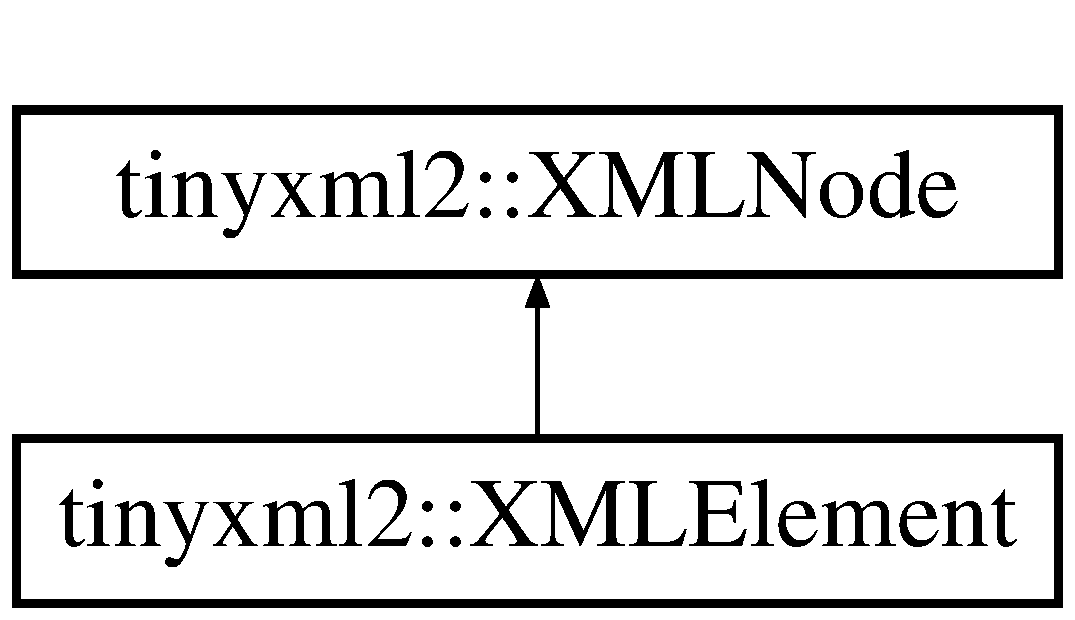
\includegraphics[height=2.000000cm]{classtinyxml2_1_1_x_m_l_element}
\end{center}
\end{figure}
\subsection*{Public Types}
\begin{DoxyCompactItemize}
\item 
enum \{ \hyperlink{classtinyxml2_1_1_x_m_l_element_a07a6ce25c17aaa505933db57f2373e50a78cf277c55b4655c86458dfecb11d349}{O\+P\+E\+N}, 
\hyperlink{classtinyxml2_1_1_x_m_l_element_a07a6ce25c17aaa505933db57f2373e50aa2f1f384020d2d4538ad2ec84930a028}{C\+L\+O\+S\+E\+D}, 
\hyperlink{classtinyxml2_1_1_x_m_l_element_a07a6ce25c17aaa505933db57f2373e50aa2857344b98a931536c443cd0cadc4b7}{C\+L\+O\+S\+I\+N\+G}
 \}
\end{DoxyCompactItemize}
\subsection*{Public Member Functions}
\begin{DoxyCompactItemize}
\item 
const char $\ast$ \hyperlink{classtinyxml2_1_1_x_m_l_element_a8bff355472bce2c60d4b50a212bf7f5f}{Name} () const 
\begin{DoxyCompactList}\small\item\em Get the name of an element (which is the \hyperlink{classtinyxml2_1_1_x_m_l_node_a92835c779871918f9af569bfe9669fe6}{Value()} of the node.) \end{DoxyCompactList}\item 
void \hyperlink{classtinyxml2_1_1_x_m_l_element_a97712009a530d8cb8a63bf705f02b4f1}{Set\+Name} (const char $\ast$str, bool static\+Mem=false)
\begin{DoxyCompactList}\small\item\em Set the name of the element. \end{DoxyCompactList}\item 
virtual \hyperlink{classtinyxml2_1_1_x_m_l_element}{X\+M\+L\+Element} $\ast$ \hyperlink{classtinyxml2_1_1_x_m_l_element_ad9ff5c2dbc15df36cf664ce1b0ea0a5d}{To\+Element} ()
\begin{DoxyCompactList}\small\item\em Safely cast to an Element, or null. \end{DoxyCompactList}\item 
virtual const \hyperlink{classtinyxml2_1_1_x_m_l_element}{X\+M\+L\+Element} $\ast$ \hyperlink{classtinyxml2_1_1_x_m_l_element_a55acab615353ddabab48271f95816b0d}{To\+Element} () const 
\item 
virtual bool \hyperlink{classtinyxml2_1_1_x_m_l_element_a36d65438991a1e85096caf39ad13a099}{Accept} (\hyperlink{classtinyxml2_1_1_x_m_l_visitor}{X\+M\+L\+Visitor} $\ast$visitor) const 
\item 
const char $\ast$ \hyperlink{classtinyxml2_1_1_x_m_l_element_a7bdebdf1888074087237f3dd03912740}{Attribute} (const char $\ast$name, const char $\ast$value=0) const 
\item 
int \hyperlink{classtinyxml2_1_1_x_m_l_element_af86f05771c11a73a2896b662bb589ef5}{Int\+Attribute} (const char $\ast$name) const 
\item 
unsigned \hyperlink{classtinyxml2_1_1_x_m_l_element_aa5a41367b5118acec42a87f5f94cec2d}{Unsigned\+Attribute} (const char $\ast$name) const 
\begin{DoxyCompactList}\small\item\em See \hyperlink{classtinyxml2_1_1_x_m_l_element_af86f05771c11a73a2896b662bb589ef5}{Int\+Attribute()} \end{DoxyCompactList}\item 
bool \hyperlink{classtinyxml2_1_1_x_m_l_element_a34811e4d1881e4ecc95c49f0f3799115}{Bool\+Attribute} (const char $\ast$name) const 
\begin{DoxyCompactList}\small\item\em See \hyperlink{classtinyxml2_1_1_x_m_l_element_af86f05771c11a73a2896b662bb589ef5}{Int\+Attribute()} \end{DoxyCompactList}\item 
double \hyperlink{classtinyxml2_1_1_x_m_l_element_a536922a5cae9c9769a3dc1b7a8ff0d44}{Double\+Attribute} (const char $\ast$name) const 
\begin{DoxyCompactList}\small\item\em See \hyperlink{classtinyxml2_1_1_x_m_l_element_af86f05771c11a73a2896b662bb589ef5}{Int\+Attribute()} \end{DoxyCompactList}\item 
float \hyperlink{classtinyxml2_1_1_x_m_l_element_a33b69f123f995aff966d2e351bc51b1f}{Float\+Attribute} (const char $\ast$name) const 
\begin{DoxyCompactList}\small\item\em See \hyperlink{classtinyxml2_1_1_x_m_l_element_af86f05771c11a73a2896b662bb589ef5}{Int\+Attribute()} \end{DoxyCompactList}\item 
\hyperlink{namespacetinyxml2_a1fbf88509c3ac88c09117b1947414e08}{X\+M\+L\+Error} \hyperlink{classtinyxml2_1_1_x_m_l_element_a8b92c729346aa8ea9acd59ed3e9f2378}{Query\+Int\+Attribute} (const char $\ast$name, int $\ast$value) const 
\item 
\hyperlink{namespacetinyxml2_a1fbf88509c3ac88c09117b1947414e08}{X\+M\+L\+Error} \hyperlink{classtinyxml2_1_1_x_m_l_element_aa3d8d1b9311da8fc249b4352749aaa84}{Query\+Unsigned\+Attribute} (const char $\ast$name, unsigned int $\ast$value) const 
\begin{DoxyCompactList}\small\item\em See \hyperlink{classtinyxml2_1_1_x_m_l_element_a8b92c729346aa8ea9acd59ed3e9f2378}{Query\+Int\+Attribute()} \end{DoxyCompactList}\item 
\hyperlink{namespacetinyxml2_a1fbf88509c3ac88c09117b1947414e08}{X\+M\+L\+Error} \hyperlink{classtinyxml2_1_1_x_m_l_element_a2a58ee941c3cda23772c887a8f8b534e}{Query\+Bool\+Attribute} (const char $\ast$name, bool $\ast$value) const 
\begin{DoxyCompactList}\small\item\em See \hyperlink{classtinyxml2_1_1_x_m_l_element_a8b92c729346aa8ea9acd59ed3e9f2378}{Query\+Int\+Attribute()} \end{DoxyCompactList}\item 
\hyperlink{namespacetinyxml2_a1fbf88509c3ac88c09117b1947414e08}{X\+M\+L\+Error} \hyperlink{classtinyxml2_1_1_x_m_l_element_a1ffeed461d3e4020b39652cd6d3cd773}{Query\+Double\+Attribute} (const char $\ast$name, double $\ast$value) const 
\begin{DoxyCompactList}\small\item\em See \hyperlink{classtinyxml2_1_1_x_m_l_element_a8b92c729346aa8ea9acd59ed3e9f2378}{Query\+Int\+Attribute()} \end{DoxyCompactList}\item 
\hyperlink{namespacetinyxml2_a1fbf88509c3ac88c09117b1947414e08}{X\+M\+L\+Error} \hyperlink{classtinyxml2_1_1_x_m_l_element_a3f154e0b4b6903249ff9f758921758e5}{Query\+Float\+Attribute} (const char $\ast$name, float $\ast$value) const 
\begin{DoxyCompactList}\small\item\em See \hyperlink{classtinyxml2_1_1_x_m_l_element_a8b92c729346aa8ea9acd59ed3e9f2378}{Query\+Int\+Attribute()} \end{DoxyCompactList}\item 
int \hyperlink{classtinyxml2_1_1_x_m_l_element_aa471a199af9f137ef371f5db1ed1016b}{Query\+Attribute} (const char $\ast$name, int $\ast$value) const 
\item 
int \hyperlink{classtinyxml2_1_1_x_m_l_element_a60d18656aa70adb257eab18913aa4330}{Query\+Attribute} (const char $\ast$name, unsigned int $\ast$value) const 
\item 
int \hyperlink{classtinyxml2_1_1_x_m_l_element_a23fa8bac4250249c476c6bfdb6cb9b9c}{Query\+Attribute} (const char $\ast$name, bool $\ast$value) const 
\item 
int \hyperlink{classtinyxml2_1_1_x_m_l_element_a64aadcbf27423410e2896baf240f63f9}{Query\+Attribute} (const char $\ast$name, double $\ast$value) const 
\item 
int \hyperlink{classtinyxml2_1_1_x_m_l_element_afd553774be0e7760d73003058efa8df9}{Query\+Attribute} (const char $\ast$name, float $\ast$value) const 
\item 
void \hyperlink{classtinyxml2_1_1_x_m_l_element_a11943abf2d0831548c3790dd5d9f119c}{Set\+Attribute} (const char $\ast$name, const char $\ast$value)
\begin{DoxyCompactList}\small\item\em Sets the named attribute to value. \end{DoxyCompactList}\item 
void \hyperlink{classtinyxml2_1_1_x_m_l_element_aae6568c64c7f1cc88be8461ba41a79cf}{Set\+Attribute} (const char $\ast$name, int value)
\begin{DoxyCompactList}\small\item\em Sets the named attribute to value. \end{DoxyCompactList}\item 
void \hyperlink{classtinyxml2_1_1_x_m_l_element_ae143997e90064ba82326b29a9930ea8f}{Set\+Attribute} (const char $\ast$name, unsigned value)
\begin{DoxyCompactList}\small\item\em Sets the named attribute to value. \end{DoxyCompactList}\item 
void \hyperlink{classtinyxml2_1_1_x_m_l_element_aa848b696e6a75e4e545c6da9893b11e1}{Set\+Attribute} (const char $\ast$name, bool value)
\begin{DoxyCompactList}\small\item\em Sets the named attribute to value. \end{DoxyCompactList}\item 
void \hyperlink{classtinyxml2_1_1_x_m_l_element_a233397ee81e70eb5d4b814c5f8698533}{Set\+Attribute} (const char $\ast$name, double value)
\begin{DoxyCompactList}\small\item\em Sets the named attribute to value. \end{DoxyCompactList}\item 
void \hyperlink{classtinyxml2_1_1_x_m_l_element_a554b70d882e65b28fc084b23df9b9759}{Set\+Attribute} (const char $\ast$name, float value)
\begin{DoxyCompactList}\small\item\em Sets the named attribute to value. \end{DoxyCompactList}\item 
void \hyperlink{classtinyxml2_1_1_x_m_l_element_aebd45aa7118964c30b32fe12e944628a}{Delete\+Attribute} (const char $\ast$name)
\item 
const \hyperlink{classtinyxml2_1_1_x_m_l_attribute}{X\+M\+L\+Attribute} $\ast$ \hyperlink{classtinyxml2_1_1_x_m_l_element_a67593e63558ffda0386699c3e4cc0b2c}{First\+Attribute} () const 
\begin{DoxyCompactList}\small\item\em Return the first attribute in the list. \end{DoxyCompactList}\item 
const \hyperlink{classtinyxml2_1_1_x_m_l_attribute}{X\+M\+L\+Attribute} $\ast$ \hyperlink{classtinyxml2_1_1_x_m_l_element_aaf46b0799ea419e5d070ac9a357de48f}{Find\+Attribute} (const char $\ast$name) const 
\begin{DoxyCompactList}\small\item\em Query a specific attribute in the list. \end{DoxyCompactList}\item 
const char $\ast$ \hyperlink{classtinyxml2_1_1_x_m_l_element_a56cc727044dad002b978256754d43a4b}{Get\+Text} () const 
\item 
void \hyperlink{classtinyxml2_1_1_x_m_l_element_a1f9c2cd61b72af5ae708d37b7ad283ce}{Set\+Text} (const char $\ast$in\+Text)
\item 
void \hyperlink{classtinyxml2_1_1_x_m_l_element_aeae8917b5ea6060b3c08d4e3d8d632d7}{Set\+Text} (int value)
\begin{DoxyCompactList}\small\item\em Convenience method for setting text inside and element. See \hyperlink{classtinyxml2_1_1_x_m_l_element_a1f9c2cd61b72af5ae708d37b7ad283ce}{Set\+Text()} for important limitations. \end{DoxyCompactList}\item 
void \hyperlink{classtinyxml2_1_1_x_m_l_element_a7bbfcc11d516598bc924a8fba4d08597}{Set\+Text} (unsigned value)
\begin{DoxyCompactList}\small\item\em Convenience method for setting text inside and element. See \hyperlink{classtinyxml2_1_1_x_m_l_element_a1f9c2cd61b72af5ae708d37b7ad283ce}{Set\+Text()} for important limitations. \end{DoxyCompactList}\item 
void \hyperlink{classtinyxml2_1_1_x_m_l_element_ae4b543d6770de76fb6ab68e541c192a4}{Set\+Text} (bool value)
\begin{DoxyCompactList}\small\item\em Convenience method for setting text inside and element. See \hyperlink{classtinyxml2_1_1_x_m_l_element_a1f9c2cd61b72af5ae708d37b7ad283ce}{Set\+Text()} for important limitations. \end{DoxyCompactList}\item 
void \hyperlink{classtinyxml2_1_1_x_m_l_element_a67bd77ac9aaeff58ff20b4275a65ba4e}{Set\+Text} (double value)
\begin{DoxyCompactList}\small\item\em Convenience method for setting text inside and element. See \hyperlink{classtinyxml2_1_1_x_m_l_element_a1f9c2cd61b72af5ae708d37b7ad283ce}{Set\+Text()} for important limitations. \end{DoxyCompactList}\item 
void \hyperlink{classtinyxml2_1_1_x_m_l_element_a51d560da5ae3ad6b75e0ab9ffb2ae42a}{Set\+Text} (float value)
\begin{DoxyCompactList}\small\item\em Convenience method for setting text inside and element. See \hyperlink{classtinyxml2_1_1_x_m_l_element_a1f9c2cd61b72af5ae708d37b7ad283ce}{Set\+Text()} for important limitations. \end{DoxyCompactList}\item 
\hyperlink{namespacetinyxml2_a1fbf88509c3ac88c09117b1947414e08}{X\+M\+L\+Error} \hyperlink{classtinyxml2_1_1_x_m_l_element_a71327c9a9d8840562bd204f46d0a7189}{Query\+Int\+Text} (int $\ast$ival) const 
\item 
\hyperlink{namespacetinyxml2_a1fbf88509c3ac88c09117b1947414e08}{X\+M\+L\+Error} \hyperlink{classtinyxml2_1_1_x_m_l_element_a2192091dec0c06be8b14f4e912c01758}{Query\+Unsigned\+Text} (unsigned $\ast$uval) const 
\begin{DoxyCompactList}\small\item\em See \hyperlink{classtinyxml2_1_1_x_m_l_element_a71327c9a9d8840562bd204f46d0a7189}{Query\+Int\+Text()} \end{DoxyCompactList}\item 
\hyperlink{namespacetinyxml2_a1fbf88509c3ac88c09117b1947414e08}{X\+M\+L\+Error} \hyperlink{classtinyxml2_1_1_x_m_l_element_afeb060672fa934163fc573e692b7fe38}{Query\+Bool\+Text} (bool $\ast$bval) const 
\begin{DoxyCompactList}\small\item\em See \hyperlink{classtinyxml2_1_1_x_m_l_element_a71327c9a9d8840562bd204f46d0a7189}{Query\+Int\+Text()} \end{DoxyCompactList}\item 
\hyperlink{namespacetinyxml2_a1fbf88509c3ac88c09117b1947414e08}{X\+M\+L\+Error} \hyperlink{classtinyxml2_1_1_x_m_l_element_aad931c42548907dbea416f7365d78b57}{Query\+Double\+Text} (double $\ast$dval) const 
\begin{DoxyCompactList}\small\item\em See \hyperlink{classtinyxml2_1_1_x_m_l_element_a71327c9a9d8840562bd204f46d0a7189}{Query\+Int\+Text()} \end{DoxyCompactList}\item 
\hyperlink{namespacetinyxml2_a1fbf88509c3ac88c09117b1947414e08}{X\+M\+L\+Error} \hyperlink{classtinyxml2_1_1_x_m_l_element_a11fa26e1dbca88e973964c1d9b597658}{Query\+Float\+Text} (float $\ast$fval) const 
\begin{DoxyCompactList}\small\item\em See \hyperlink{classtinyxml2_1_1_x_m_l_element_a71327c9a9d8840562bd204f46d0a7189}{Query\+Int\+Text()} \end{DoxyCompactList}\item 
int \hyperlink{classtinyxml2_1_1_x_m_l_element_a2e3d9f938307a05963d7c4b8cd55754e}{Closing\+Type} () const 
\item 
char $\ast$ \hyperlink{classtinyxml2_1_1_x_m_l_element_aaafdd2a5618abe80a2c1839ad3ccd492}{Parse\+Deep} (char $\ast$p, \hyperlink{classtinyxml2_1_1_str_pair}{Str\+Pair} $\ast$end\+Tag)
\item 
virtual \hyperlink{classtinyxml2_1_1_x_m_l_node}{X\+M\+L\+Node} $\ast$ \hyperlink{classtinyxml2_1_1_x_m_l_element_a85d85e32c18863fff1eeed53ae1ce23d}{Shallow\+Clone} (\hyperlink{classtinyxml2_1_1_x_m_l_document}{X\+M\+L\+Document} $\ast$document) const 
\item 
virtual bool \hyperlink{classtinyxml2_1_1_x_m_l_element_a25d51a2aad92625c78441457d58c85bc}{Shallow\+Equal} (const \hyperlink{classtinyxml2_1_1_x_m_l_node}{X\+M\+L\+Node} $\ast$compare) const 
\end{DoxyCompactItemize}
\subsection*{Friends}
\begin{DoxyCompactItemize}
\item 
class \hyperlink{classtinyxml2_1_1_x_m_l_element_a449202cfc89e7ae5c2f81995476f9ec1}{X\+M\+L\+Base}
\item 
class \hyperlink{classtinyxml2_1_1_x_m_l_element_a4eee3bda60c60a30e4e8cd4ea91c4c6e}{X\+M\+L\+Document}
\end{DoxyCompactItemize}
\subsection*{Additional Inherited Members}


\subsection{Detailed Description}
The element is a container class. It has a value, the element name, and can contain other elements, text, comments, and unknowns. Elements also contain an arbitrary number of attributes. 

\subsection{Member Enumeration Documentation}
\hypertarget{classtinyxml2_1_1_x_m_l_element_a07a6ce25c17aaa505933db57f2373e50}{}\subsubsection[{anonymous enum}]{\setlength{\rightskip}{0pt plus 5cm}anonymous enum}\label{classtinyxml2_1_1_x_m_l_element_a07a6ce25c17aaa505933db57f2373e50}
\begin{Desc}
\item[Enumerator]\par
\begin{description}
\index{O\+P\+E\+N@{O\+P\+E\+N}!tinyxml2\+::\+X\+M\+L\+Element@{tinyxml2\+::\+X\+M\+L\+Element}}\index{tinyxml2\+::\+X\+M\+L\+Element@{tinyxml2\+::\+X\+M\+L\+Element}!O\+P\+E\+N@{O\+P\+E\+N}}\item[{\em 
\hypertarget{classtinyxml2_1_1_x_m_l_element_a07a6ce25c17aaa505933db57f2373e50a78cf277c55b4655c86458dfecb11d349}{}O\+P\+E\+N\label{classtinyxml2_1_1_x_m_l_element_a07a6ce25c17aaa505933db57f2373e50a78cf277c55b4655c86458dfecb11d349}
}]\index{C\+L\+O\+S\+E\+D@{C\+L\+O\+S\+E\+D}!tinyxml2\+::\+X\+M\+L\+Element@{tinyxml2\+::\+X\+M\+L\+Element}}\index{tinyxml2\+::\+X\+M\+L\+Element@{tinyxml2\+::\+X\+M\+L\+Element}!C\+L\+O\+S\+E\+D@{C\+L\+O\+S\+E\+D}}\item[{\em 
\hypertarget{classtinyxml2_1_1_x_m_l_element_a07a6ce25c17aaa505933db57f2373e50aa2f1f384020d2d4538ad2ec84930a028}{}C\+L\+O\+S\+E\+D\label{classtinyxml2_1_1_x_m_l_element_a07a6ce25c17aaa505933db57f2373e50aa2f1f384020d2d4538ad2ec84930a028}
}]\index{C\+L\+O\+S\+I\+N\+G@{C\+L\+O\+S\+I\+N\+G}!tinyxml2\+::\+X\+M\+L\+Element@{tinyxml2\+::\+X\+M\+L\+Element}}\index{tinyxml2\+::\+X\+M\+L\+Element@{tinyxml2\+::\+X\+M\+L\+Element}!C\+L\+O\+S\+I\+N\+G@{C\+L\+O\+S\+I\+N\+G}}\item[{\em 
\hypertarget{classtinyxml2_1_1_x_m_l_element_a07a6ce25c17aaa505933db57f2373e50aa2857344b98a931536c443cd0cadc4b7}{}C\+L\+O\+S\+I\+N\+G\label{classtinyxml2_1_1_x_m_l_element_a07a6ce25c17aaa505933db57f2373e50aa2857344b98a931536c443cd0cadc4b7}
}]\end{description}
\end{Desc}


\subsection{Member Function Documentation}
\hypertarget{classtinyxml2_1_1_x_m_l_element_a36d65438991a1e85096caf39ad13a099}{}\index{tinyxml2\+::\+X\+M\+L\+Element@{tinyxml2\+::\+X\+M\+L\+Element}!Accept@{Accept}}
\index{Accept@{Accept}!tinyxml2\+::\+X\+M\+L\+Element@{tinyxml2\+::\+X\+M\+L\+Element}}
\subsubsection[{Accept}]{\setlength{\rightskip}{0pt plus 5cm}bool tinyxml2\+::\+X\+M\+L\+Element\+::\+Accept (
\begin{DoxyParamCaption}
\item[{{\bf X\+M\+L\+Visitor} $\ast$}]{visitor}
\end{DoxyParamCaption}
) const\hspace{0.3cm}{\ttfamily [virtual]}}\label{classtinyxml2_1_1_x_m_l_element_a36d65438991a1e85096caf39ad13a099}
Accept a hierarchical visit of the nodes in the Tiny\+X\+M\+L-\/2 D\+O\+M. Every node in the X\+M\+L tree will be conditionally visited and the host will be called back via the \hyperlink{classtinyxml2_1_1_x_m_l_visitor}{X\+M\+L\+Visitor} interface.

This is essentially a S\+A\+X interface for Tiny\+X\+M\+L-\/2. (Note however it doesn\textquotesingle{}t re-\/parse the X\+M\+L for the callbacks, so the performance of Tiny\+X\+M\+L-\/2 is unchanged by using this interface versus any other.)

The interface has been based on ideas from\+:


\begin{DoxyItemize}
\item \href{http://www.saxproject.org/}{\tt http\+://www.\+saxproject.\+org/}
\item \href{http://c2.com/cgi/wiki?HierarchicalVisitorPattern}{\tt http\+://c2.\+com/cgi/wiki?\+Hierarchical\+Visitor\+Pattern}
\end{DoxyItemize}

Which are both good references for \char`\"{}visiting\char`\"{}.

An example of using \hyperlink{classtinyxml2_1_1_x_m_l_element_a36d65438991a1e85096caf39ad13a099}{Accept()}\+: \begin{DoxyVerb}XMLPrinter printer;
tinyxmlDoc.Accept( &printer );
const char* xmlcstr = printer.CStr();
\end{DoxyVerb}
 

Implements \hyperlink{classtinyxml2_1_1_x_m_l_node_a81e66df0a44c67a7af17f3b77a152785}{tinyxml2\+::\+X\+M\+L\+Node}.

\hypertarget{classtinyxml2_1_1_x_m_l_element_a7bdebdf1888074087237f3dd03912740}{}\index{tinyxml2\+::\+X\+M\+L\+Element@{tinyxml2\+::\+X\+M\+L\+Element}!Attribute@{Attribute}}
\index{Attribute@{Attribute}!tinyxml2\+::\+X\+M\+L\+Element@{tinyxml2\+::\+X\+M\+L\+Element}}
\subsubsection[{Attribute}]{\setlength{\rightskip}{0pt plus 5cm}const char $\ast$ tinyxml2\+::\+X\+M\+L\+Element\+::\+Attribute (
\begin{DoxyParamCaption}
\item[{const char $\ast$}]{name, }
\item[{const char $\ast$}]{value = {\ttfamily 0}}
\end{DoxyParamCaption}
) const}\label{classtinyxml2_1_1_x_m_l_element_a7bdebdf1888074087237f3dd03912740}
Given an attribute name, \hyperlink{classtinyxml2_1_1_x_m_l_element_a7bdebdf1888074087237f3dd03912740}{Attribute()} returns the value for the attribute of that name, or null if none exists. For example\+:

\begin{DoxyVerb}const char* value = ele->Attribute( "foo" );
\end{DoxyVerb}


The \textquotesingle{}value\textquotesingle{} parameter is normally null. However, if specified, the attribute will only be returned if the \textquotesingle{}name\textquotesingle{} and \textquotesingle{}value\textquotesingle{} match. This allow you to write code\+:

\begin{DoxyVerb}if ( ele->Attribute( "foo", "bar" ) ) callFooIsBar();
\end{DoxyVerb}


rather than\+: \begin{DoxyVerb}if ( ele->Attribute( "foo" ) ) {
    if ( strcmp( ele->Attribute( "foo" ), "bar" ) == 0 ) callFooIsBar();
}
\end{DoxyVerb}
 \hypertarget{classtinyxml2_1_1_x_m_l_element_a34811e4d1881e4ecc95c49f0f3799115}{}\index{tinyxml2\+::\+X\+M\+L\+Element@{tinyxml2\+::\+X\+M\+L\+Element}!Bool\+Attribute@{Bool\+Attribute}}
\index{Bool\+Attribute@{Bool\+Attribute}!tinyxml2\+::\+X\+M\+L\+Element@{tinyxml2\+::\+X\+M\+L\+Element}}
\subsubsection[{Bool\+Attribute}]{\setlength{\rightskip}{0pt plus 5cm}bool tinyxml2\+::\+X\+M\+L\+Element\+::\+Bool\+Attribute (
\begin{DoxyParamCaption}
\item[{const char $\ast$}]{name}
\end{DoxyParamCaption}
) const\hspace{0.3cm}{\ttfamily [inline]}}\label{classtinyxml2_1_1_x_m_l_element_a34811e4d1881e4ecc95c49f0f3799115}


See \hyperlink{classtinyxml2_1_1_x_m_l_element_af86f05771c11a73a2896b662bb589ef5}{Int\+Attribute()} 

\hypertarget{classtinyxml2_1_1_x_m_l_element_a2e3d9f938307a05963d7c4b8cd55754e}{}\index{tinyxml2\+::\+X\+M\+L\+Element@{tinyxml2\+::\+X\+M\+L\+Element}!Closing\+Type@{Closing\+Type}}
\index{Closing\+Type@{Closing\+Type}!tinyxml2\+::\+X\+M\+L\+Element@{tinyxml2\+::\+X\+M\+L\+Element}}
\subsubsection[{Closing\+Type}]{\setlength{\rightskip}{0pt plus 5cm}int tinyxml2\+::\+X\+M\+L\+Element\+::\+Closing\+Type (
\begin{DoxyParamCaption}
{}
\end{DoxyParamCaption}
) const\hspace{0.3cm}{\ttfamily [inline]}}\label{classtinyxml2_1_1_x_m_l_element_a2e3d9f938307a05963d7c4b8cd55754e}
\hypertarget{classtinyxml2_1_1_x_m_l_element_aebd45aa7118964c30b32fe12e944628a}{}\index{tinyxml2\+::\+X\+M\+L\+Element@{tinyxml2\+::\+X\+M\+L\+Element}!Delete\+Attribute@{Delete\+Attribute}}
\index{Delete\+Attribute@{Delete\+Attribute}!tinyxml2\+::\+X\+M\+L\+Element@{tinyxml2\+::\+X\+M\+L\+Element}}
\subsubsection[{Delete\+Attribute}]{\setlength{\rightskip}{0pt plus 5cm}void tinyxml2\+::\+X\+M\+L\+Element\+::\+Delete\+Attribute (
\begin{DoxyParamCaption}
\item[{const char $\ast$}]{name}
\end{DoxyParamCaption}
)}\label{classtinyxml2_1_1_x_m_l_element_aebd45aa7118964c30b32fe12e944628a}
Delete an attribute. \hypertarget{classtinyxml2_1_1_x_m_l_element_a536922a5cae9c9769a3dc1b7a8ff0d44}{}\index{tinyxml2\+::\+X\+M\+L\+Element@{tinyxml2\+::\+X\+M\+L\+Element}!Double\+Attribute@{Double\+Attribute}}
\index{Double\+Attribute@{Double\+Attribute}!tinyxml2\+::\+X\+M\+L\+Element@{tinyxml2\+::\+X\+M\+L\+Element}}
\subsubsection[{Double\+Attribute}]{\setlength{\rightskip}{0pt plus 5cm}double tinyxml2\+::\+X\+M\+L\+Element\+::\+Double\+Attribute (
\begin{DoxyParamCaption}
\item[{const char $\ast$}]{name}
\end{DoxyParamCaption}
) const\hspace{0.3cm}{\ttfamily [inline]}}\label{classtinyxml2_1_1_x_m_l_element_a536922a5cae9c9769a3dc1b7a8ff0d44}


See \hyperlink{classtinyxml2_1_1_x_m_l_element_af86f05771c11a73a2896b662bb589ef5}{Int\+Attribute()} 

\hypertarget{classtinyxml2_1_1_x_m_l_element_aaf46b0799ea419e5d070ac9a357de48f}{}\index{tinyxml2\+::\+X\+M\+L\+Element@{tinyxml2\+::\+X\+M\+L\+Element}!Find\+Attribute@{Find\+Attribute}}
\index{Find\+Attribute@{Find\+Attribute}!tinyxml2\+::\+X\+M\+L\+Element@{tinyxml2\+::\+X\+M\+L\+Element}}
\subsubsection[{Find\+Attribute}]{\setlength{\rightskip}{0pt plus 5cm}const {\bf X\+M\+L\+Attribute} $\ast$ tinyxml2\+::\+X\+M\+L\+Element\+::\+Find\+Attribute (
\begin{DoxyParamCaption}
\item[{const char $\ast$}]{name}
\end{DoxyParamCaption}
) const}\label{classtinyxml2_1_1_x_m_l_element_aaf46b0799ea419e5d070ac9a357de48f}


Query a specific attribute in the list. 

\hypertarget{classtinyxml2_1_1_x_m_l_element_a67593e63558ffda0386699c3e4cc0b2c}{}\index{tinyxml2\+::\+X\+M\+L\+Element@{tinyxml2\+::\+X\+M\+L\+Element}!First\+Attribute@{First\+Attribute}}
\index{First\+Attribute@{First\+Attribute}!tinyxml2\+::\+X\+M\+L\+Element@{tinyxml2\+::\+X\+M\+L\+Element}}
\subsubsection[{First\+Attribute}]{\setlength{\rightskip}{0pt plus 5cm}const {\bf X\+M\+L\+Attribute}$\ast$ tinyxml2\+::\+X\+M\+L\+Element\+::\+First\+Attribute (
\begin{DoxyParamCaption}
{}
\end{DoxyParamCaption}
) const\hspace{0.3cm}{\ttfamily [inline]}}\label{classtinyxml2_1_1_x_m_l_element_a67593e63558ffda0386699c3e4cc0b2c}


Return the first attribute in the list. 

\hypertarget{classtinyxml2_1_1_x_m_l_element_a33b69f123f995aff966d2e351bc51b1f}{}\index{tinyxml2\+::\+X\+M\+L\+Element@{tinyxml2\+::\+X\+M\+L\+Element}!Float\+Attribute@{Float\+Attribute}}
\index{Float\+Attribute@{Float\+Attribute}!tinyxml2\+::\+X\+M\+L\+Element@{tinyxml2\+::\+X\+M\+L\+Element}}
\subsubsection[{Float\+Attribute}]{\setlength{\rightskip}{0pt plus 5cm}float tinyxml2\+::\+X\+M\+L\+Element\+::\+Float\+Attribute (
\begin{DoxyParamCaption}
\item[{const char $\ast$}]{name}
\end{DoxyParamCaption}
) const\hspace{0.3cm}{\ttfamily [inline]}}\label{classtinyxml2_1_1_x_m_l_element_a33b69f123f995aff966d2e351bc51b1f}


See \hyperlink{classtinyxml2_1_1_x_m_l_element_af86f05771c11a73a2896b662bb589ef5}{Int\+Attribute()} 

\hypertarget{classtinyxml2_1_1_x_m_l_element_a56cc727044dad002b978256754d43a4b}{}\index{tinyxml2\+::\+X\+M\+L\+Element@{tinyxml2\+::\+X\+M\+L\+Element}!Get\+Text@{Get\+Text}}
\index{Get\+Text@{Get\+Text}!tinyxml2\+::\+X\+M\+L\+Element@{tinyxml2\+::\+X\+M\+L\+Element}}
\subsubsection[{Get\+Text}]{\setlength{\rightskip}{0pt plus 5cm}const char $\ast$ tinyxml2\+::\+X\+M\+L\+Element\+::\+Get\+Text (
\begin{DoxyParamCaption}
{}
\end{DoxyParamCaption}
) const}\label{classtinyxml2_1_1_x_m_l_element_a56cc727044dad002b978256754d43a4b}
Convenience function for easy access to the text inside an element. Although easy and concise, \hyperlink{classtinyxml2_1_1_x_m_l_element_a56cc727044dad002b978256754d43a4b}{Get\+Text()} is limited compared to getting the \hyperlink{classtinyxml2_1_1_x_m_l_text}{X\+M\+L\+Text} child and accessing it directly.

If the first child of \textquotesingle{}this\textquotesingle{} is a \hyperlink{classtinyxml2_1_1_x_m_l_text}{X\+M\+L\+Text}, the \hyperlink{classtinyxml2_1_1_x_m_l_element_a56cc727044dad002b978256754d43a4b}{Get\+Text()} returns the character string of the Text node, else null is returned.

This is a convenient method for getting the text of simple contained text\+: \begin{DoxyVerb}<foo>This is text</foo>
    const char* str = fooElement->GetText();
\end{DoxyVerb}


\textquotesingle{}str\textquotesingle{} will be a pointer to \char`\"{}\+This is text\char`\"{}.

Note that this function can be misleading. If the element foo was created from this X\+M\+L\+: \begin{DoxyVerb}    <foo><b>This is text</b></foo>
\end{DoxyVerb}


then the value of str would be null. The first child node isn\textquotesingle{}t a text node, it is another element. From this X\+M\+L\+: \begin{DoxyVerb}    <foo>This is <b>text</b></foo>
\end{DoxyVerb}
 \hyperlink{classtinyxml2_1_1_x_m_l_element_a56cc727044dad002b978256754d43a4b}{Get\+Text()} will return \char`\"{}\+This is \char`\"{}. \hypertarget{classtinyxml2_1_1_x_m_l_element_af86f05771c11a73a2896b662bb589ef5}{}\index{tinyxml2\+::\+X\+M\+L\+Element@{tinyxml2\+::\+X\+M\+L\+Element}!Int\+Attribute@{Int\+Attribute}}
\index{Int\+Attribute@{Int\+Attribute}!tinyxml2\+::\+X\+M\+L\+Element@{tinyxml2\+::\+X\+M\+L\+Element}}
\subsubsection[{Int\+Attribute}]{\setlength{\rightskip}{0pt plus 5cm}int tinyxml2\+::\+X\+M\+L\+Element\+::\+Int\+Attribute (
\begin{DoxyParamCaption}
\item[{const char $\ast$}]{name}
\end{DoxyParamCaption}
) const\hspace{0.3cm}{\ttfamily [inline]}}\label{classtinyxml2_1_1_x_m_l_element_af86f05771c11a73a2896b662bb589ef5}
Given an attribute name, \hyperlink{classtinyxml2_1_1_x_m_l_element_af86f05771c11a73a2896b662bb589ef5}{Int\+Attribute()} returns the value of the attribute interpreted as an integer. 0 will be returned if there is an error. For a method with error checking, see \hyperlink{classtinyxml2_1_1_x_m_l_element_a8b92c729346aa8ea9acd59ed3e9f2378}{Query\+Int\+Attribute()} \hypertarget{classtinyxml2_1_1_x_m_l_element_a8bff355472bce2c60d4b50a212bf7f5f}{}\index{tinyxml2\+::\+X\+M\+L\+Element@{tinyxml2\+::\+X\+M\+L\+Element}!Name@{Name}}
\index{Name@{Name}!tinyxml2\+::\+X\+M\+L\+Element@{tinyxml2\+::\+X\+M\+L\+Element}}
\subsubsection[{Name}]{\setlength{\rightskip}{0pt plus 5cm}const char$\ast$ tinyxml2\+::\+X\+M\+L\+Element\+::\+Name (
\begin{DoxyParamCaption}
{}
\end{DoxyParamCaption}
) const\hspace{0.3cm}{\ttfamily [inline]}}\label{classtinyxml2_1_1_x_m_l_element_a8bff355472bce2c60d4b50a212bf7f5f}


Get the name of an element (which is the \hyperlink{classtinyxml2_1_1_x_m_l_node_a92835c779871918f9af569bfe9669fe6}{Value()} of the node.) 

\hypertarget{classtinyxml2_1_1_x_m_l_element_aaafdd2a5618abe80a2c1839ad3ccd492}{}\index{tinyxml2\+::\+X\+M\+L\+Element@{tinyxml2\+::\+X\+M\+L\+Element}!Parse\+Deep@{Parse\+Deep}}
\index{Parse\+Deep@{Parse\+Deep}!tinyxml2\+::\+X\+M\+L\+Element@{tinyxml2\+::\+X\+M\+L\+Element}}
\subsubsection[{Parse\+Deep}]{\setlength{\rightskip}{0pt plus 5cm}char $\ast$ tinyxml2\+::\+X\+M\+L\+Element\+::\+Parse\+Deep (
\begin{DoxyParamCaption}
\item[{char $\ast$}]{p, }
\item[{{\bf Str\+Pair} $\ast$}]{end\+Tag}
\end{DoxyParamCaption}
)\hspace{0.3cm}{\ttfamily [virtual]}}\label{classtinyxml2_1_1_x_m_l_element_aaafdd2a5618abe80a2c1839ad3ccd492}


Reimplemented from \hyperlink{classtinyxml2_1_1_x_m_l_node_a7610d0f603e8b603d2078521811a23c1}{tinyxml2\+::\+X\+M\+L\+Node}.

\hypertarget{classtinyxml2_1_1_x_m_l_element_aa471a199af9f137ef371f5db1ed1016b}{}\index{tinyxml2\+::\+X\+M\+L\+Element@{tinyxml2\+::\+X\+M\+L\+Element}!Query\+Attribute@{Query\+Attribute}}
\index{Query\+Attribute@{Query\+Attribute}!tinyxml2\+::\+X\+M\+L\+Element@{tinyxml2\+::\+X\+M\+L\+Element}}
\subsubsection[{Query\+Attribute}]{\setlength{\rightskip}{0pt plus 5cm}int tinyxml2\+::\+X\+M\+L\+Element\+::\+Query\+Attribute (
\begin{DoxyParamCaption}
\item[{const char $\ast$}]{name, }
\item[{int $\ast$}]{value}
\end{DoxyParamCaption}
) const\hspace{0.3cm}{\ttfamily [inline]}}\label{classtinyxml2_1_1_x_m_l_element_aa471a199af9f137ef371f5db1ed1016b}
Given an attribute name, \hyperlink{classtinyxml2_1_1_x_m_l_element_aa471a199af9f137ef371f5db1ed1016b}{Query\+Attribute()} returns X\+M\+L\+\_\+\+N\+O\+\_\+\+E\+R\+R\+O\+R, X\+M\+L\+\_\+\+W\+R\+O\+N\+G\+\_\+\+A\+T\+T\+R\+I\+B\+U\+T\+E\+\_\+\+T\+Y\+P\+E if the conversion can\textquotesingle{}t be performed, or X\+M\+L\+\_\+\+N\+O\+\_\+\+A\+T\+T\+R\+I\+B\+U\+T\+E if the attribute doesn\textquotesingle{}t exist. It is overloaded for the primitive types, and is a generally more convenient replacement of \hyperlink{classtinyxml2_1_1_x_m_l_element_a8b92c729346aa8ea9acd59ed3e9f2378}{Query\+Int\+Attribute()} and related functions.

If successful, the result of the conversion will be written to \textquotesingle{}value\textquotesingle{}. If not successful, nothing will be written to \textquotesingle{}value\textquotesingle{}. This allows you to provide default value\+:

\begin{DoxyVerb}int value = 10;
QueryAttribute( "foo", &value );        // if "foo" isn't found, value will still be 10
\end{DoxyVerb}
 \hypertarget{classtinyxml2_1_1_x_m_l_element_a60d18656aa70adb257eab18913aa4330}{}\index{tinyxml2\+::\+X\+M\+L\+Element@{tinyxml2\+::\+X\+M\+L\+Element}!Query\+Attribute@{Query\+Attribute}}
\index{Query\+Attribute@{Query\+Attribute}!tinyxml2\+::\+X\+M\+L\+Element@{tinyxml2\+::\+X\+M\+L\+Element}}
\subsubsection[{Query\+Attribute}]{\setlength{\rightskip}{0pt plus 5cm}int tinyxml2\+::\+X\+M\+L\+Element\+::\+Query\+Attribute (
\begin{DoxyParamCaption}
\item[{const char $\ast$}]{name, }
\item[{unsigned int $\ast$}]{value}
\end{DoxyParamCaption}
) const\hspace{0.3cm}{\ttfamily [inline]}}\label{classtinyxml2_1_1_x_m_l_element_a60d18656aa70adb257eab18913aa4330}
\hypertarget{classtinyxml2_1_1_x_m_l_element_a23fa8bac4250249c476c6bfdb6cb9b9c}{}\index{tinyxml2\+::\+X\+M\+L\+Element@{tinyxml2\+::\+X\+M\+L\+Element}!Query\+Attribute@{Query\+Attribute}}
\index{Query\+Attribute@{Query\+Attribute}!tinyxml2\+::\+X\+M\+L\+Element@{tinyxml2\+::\+X\+M\+L\+Element}}
\subsubsection[{Query\+Attribute}]{\setlength{\rightskip}{0pt plus 5cm}int tinyxml2\+::\+X\+M\+L\+Element\+::\+Query\+Attribute (
\begin{DoxyParamCaption}
\item[{const char $\ast$}]{name, }
\item[{bool $\ast$}]{value}
\end{DoxyParamCaption}
) const\hspace{0.3cm}{\ttfamily [inline]}}\label{classtinyxml2_1_1_x_m_l_element_a23fa8bac4250249c476c6bfdb6cb9b9c}
\hypertarget{classtinyxml2_1_1_x_m_l_element_a64aadcbf27423410e2896baf240f63f9}{}\index{tinyxml2\+::\+X\+M\+L\+Element@{tinyxml2\+::\+X\+M\+L\+Element}!Query\+Attribute@{Query\+Attribute}}
\index{Query\+Attribute@{Query\+Attribute}!tinyxml2\+::\+X\+M\+L\+Element@{tinyxml2\+::\+X\+M\+L\+Element}}
\subsubsection[{Query\+Attribute}]{\setlength{\rightskip}{0pt plus 5cm}int tinyxml2\+::\+X\+M\+L\+Element\+::\+Query\+Attribute (
\begin{DoxyParamCaption}
\item[{const char $\ast$}]{name, }
\item[{double $\ast$}]{value}
\end{DoxyParamCaption}
) const\hspace{0.3cm}{\ttfamily [inline]}}\label{classtinyxml2_1_1_x_m_l_element_a64aadcbf27423410e2896baf240f63f9}
\hypertarget{classtinyxml2_1_1_x_m_l_element_afd553774be0e7760d73003058efa8df9}{}\index{tinyxml2\+::\+X\+M\+L\+Element@{tinyxml2\+::\+X\+M\+L\+Element}!Query\+Attribute@{Query\+Attribute}}
\index{Query\+Attribute@{Query\+Attribute}!tinyxml2\+::\+X\+M\+L\+Element@{tinyxml2\+::\+X\+M\+L\+Element}}
\subsubsection[{Query\+Attribute}]{\setlength{\rightskip}{0pt plus 5cm}int tinyxml2\+::\+X\+M\+L\+Element\+::\+Query\+Attribute (
\begin{DoxyParamCaption}
\item[{const char $\ast$}]{name, }
\item[{float $\ast$}]{value}
\end{DoxyParamCaption}
) const\hspace{0.3cm}{\ttfamily [inline]}}\label{classtinyxml2_1_1_x_m_l_element_afd553774be0e7760d73003058efa8df9}
\hypertarget{classtinyxml2_1_1_x_m_l_element_a2a58ee941c3cda23772c887a8f8b534e}{}\index{tinyxml2\+::\+X\+M\+L\+Element@{tinyxml2\+::\+X\+M\+L\+Element}!Query\+Bool\+Attribute@{Query\+Bool\+Attribute}}
\index{Query\+Bool\+Attribute@{Query\+Bool\+Attribute}!tinyxml2\+::\+X\+M\+L\+Element@{tinyxml2\+::\+X\+M\+L\+Element}}
\subsubsection[{Query\+Bool\+Attribute}]{\setlength{\rightskip}{0pt plus 5cm}{\bf X\+M\+L\+Error} tinyxml2\+::\+X\+M\+L\+Element\+::\+Query\+Bool\+Attribute (
\begin{DoxyParamCaption}
\item[{const char $\ast$}]{name, }
\item[{bool $\ast$}]{value}
\end{DoxyParamCaption}
) const\hspace{0.3cm}{\ttfamily [inline]}}\label{classtinyxml2_1_1_x_m_l_element_a2a58ee941c3cda23772c887a8f8b534e}


See \hyperlink{classtinyxml2_1_1_x_m_l_element_a8b92c729346aa8ea9acd59ed3e9f2378}{Query\+Int\+Attribute()} 

\hypertarget{classtinyxml2_1_1_x_m_l_element_afeb060672fa934163fc573e692b7fe38}{}\index{tinyxml2\+::\+X\+M\+L\+Element@{tinyxml2\+::\+X\+M\+L\+Element}!Query\+Bool\+Text@{Query\+Bool\+Text}}
\index{Query\+Bool\+Text@{Query\+Bool\+Text}!tinyxml2\+::\+X\+M\+L\+Element@{tinyxml2\+::\+X\+M\+L\+Element}}
\subsubsection[{Query\+Bool\+Text}]{\setlength{\rightskip}{0pt plus 5cm}{\bf X\+M\+L\+Error} tinyxml2\+::\+X\+M\+L\+Element\+::\+Query\+Bool\+Text (
\begin{DoxyParamCaption}
\item[{bool $\ast$}]{bval}
\end{DoxyParamCaption}
) const}\label{classtinyxml2_1_1_x_m_l_element_afeb060672fa934163fc573e692b7fe38}


See \hyperlink{classtinyxml2_1_1_x_m_l_element_a71327c9a9d8840562bd204f46d0a7189}{Query\+Int\+Text()} 

\hypertarget{classtinyxml2_1_1_x_m_l_element_a1ffeed461d3e4020b39652cd6d3cd773}{}\index{tinyxml2\+::\+X\+M\+L\+Element@{tinyxml2\+::\+X\+M\+L\+Element}!Query\+Double\+Attribute@{Query\+Double\+Attribute}}
\index{Query\+Double\+Attribute@{Query\+Double\+Attribute}!tinyxml2\+::\+X\+M\+L\+Element@{tinyxml2\+::\+X\+M\+L\+Element}}
\subsubsection[{Query\+Double\+Attribute}]{\setlength{\rightskip}{0pt plus 5cm}{\bf X\+M\+L\+Error} tinyxml2\+::\+X\+M\+L\+Element\+::\+Query\+Double\+Attribute (
\begin{DoxyParamCaption}
\item[{const char $\ast$}]{name, }
\item[{double $\ast$}]{value}
\end{DoxyParamCaption}
) const\hspace{0.3cm}{\ttfamily [inline]}}\label{classtinyxml2_1_1_x_m_l_element_a1ffeed461d3e4020b39652cd6d3cd773}


See \hyperlink{classtinyxml2_1_1_x_m_l_element_a8b92c729346aa8ea9acd59ed3e9f2378}{Query\+Int\+Attribute()} 

\hypertarget{classtinyxml2_1_1_x_m_l_element_aad931c42548907dbea416f7365d78b57}{}\index{tinyxml2\+::\+X\+M\+L\+Element@{tinyxml2\+::\+X\+M\+L\+Element}!Query\+Double\+Text@{Query\+Double\+Text}}
\index{Query\+Double\+Text@{Query\+Double\+Text}!tinyxml2\+::\+X\+M\+L\+Element@{tinyxml2\+::\+X\+M\+L\+Element}}
\subsubsection[{Query\+Double\+Text}]{\setlength{\rightskip}{0pt plus 5cm}{\bf X\+M\+L\+Error} tinyxml2\+::\+X\+M\+L\+Element\+::\+Query\+Double\+Text (
\begin{DoxyParamCaption}
\item[{double $\ast$}]{dval}
\end{DoxyParamCaption}
) const}\label{classtinyxml2_1_1_x_m_l_element_aad931c42548907dbea416f7365d78b57}


See \hyperlink{classtinyxml2_1_1_x_m_l_element_a71327c9a9d8840562bd204f46d0a7189}{Query\+Int\+Text()} 

\hypertarget{classtinyxml2_1_1_x_m_l_element_a3f154e0b4b6903249ff9f758921758e5}{}\index{tinyxml2\+::\+X\+M\+L\+Element@{tinyxml2\+::\+X\+M\+L\+Element}!Query\+Float\+Attribute@{Query\+Float\+Attribute}}
\index{Query\+Float\+Attribute@{Query\+Float\+Attribute}!tinyxml2\+::\+X\+M\+L\+Element@{tinyxml2\+::\+X\+M\+L\+Element}}
\subsubsection[{Query\+Float\+Attribute}]{\setlength{\rightskip}{0pt plus 5cm}{\bf X\+M\+L\+Error} tinyxml2\+::\+X\+M\+L\+Element\+::\+Query\+Float\+Attribute (
\begin{DoxyParamCaption}
\item[{const char $\ast$}]{name, }
\item[{float $\ast$}]{value}
\end{DoxyParamCaption}
) const\hspace{0.3cm}{\ttfamily [inline]}}\label{classtinyxml2_1_1_x_m_l_element_a3f154e0b4b6903249ff9f758921758e5}


See \hyperlink{classtinyxml2_1_1_x_m_l_element_a8b92c729346aa8ea9acd59ed3e9f2378}{Query\+Int\+Attribute()} 

\hypertarget{classtinyxml2_1_1_x_m_l_element_a11fa26e1dbca88e973964c1d9b597658}{}\index{tinyxml2\+::\+X\+M\+L\+Element@{tinyxml2\+::\+X\+M\+L\+Element}!Query\+Float\+Text@{Query\+Float\+Text}}
\index{Query\+Float\+Text@{Query\+Float\+Text}!tinyxml2\+::\+X\+M\+L\+Element@{tinyxml2\+::\+X\+M\+L\+Element}}
\subsubsection[{Query\+Float\+Text}]{\setlength{\rightskip}{0pt plus 5cm}{\bf X\+M\+L\+Error} tinyxml2\+::\+X\+M\+L\+Element\+::\+Query\+Float\+Text (
\begin{DoxyParamCaption}
\item[{float $\ast$}]{fval}
\end{DoxyParamCaption}
) const}\label{classtinyxml2_1_1_x_m_l_element_a11fa26e1dbca88e973964c1d9b597658}


See \hyperlink{classtinyxml2_1_1_x_m_l_element_a71327c9a9d8840562bd204f46d0a7189}{Query\+Int\+Text()} 

\hypertarget{classtinyxml2_1_1_x_m_l_element_a8b92c729346aa8ea9acd59ed3e9f2378}{}\index{tinyxml2\+::\+X\+M\+L\+Element@{tinyxml2\+::\+X\+M\+L\+Element}!Query\+Int\+Attribute@{Query\+Int\+Attribute}}
\index{Query\+Int\+Attribute@{Query\+Int\+Attribute}!tinyxml2\+::\+X\+M\+L\+Element@{tinyxml2\+::\+X\+M\+L\+Element}}
\subsubsection[{Query\+Int\+Attribute}]{\setlength{\rightskip}{0pt plus 5cm}{\bf X\+M\+L\+Error} tinyxml2\+::\+X\+M\+L\+Element\+::\+Query\+Int\+Attribute (
\begin{DoxyParamCaption}
\item[{const char $\ast$}]{name, }
\item[{int $\ast$}]{value}
\end{DoxyParamCaption}
) const\hspace{0.3cm}{\ttfamily [inline]}}\label{classtinyxml2_1_1_x_m_l_element_a8b92c729346aa8ea9acd59ed3e9f2378}
Given an attribute name, \hyperlink{classtinyxml2_1_1_x_m_l_element_a8b92c729346aa8ea9acd59ed3e9f2378}{Query\+Int\+Attribute()} returns X\+M\+L\+\_\+\+N\+O\+\_\+\+E\+R\+R\+O\+R, X\+M\+L\+\_\+\+W\+R\+O\+N\+G\+\_\+\+A\+T\+T\+R\+I\+B\+U\+T\+E\+\_\+\+T\+Y\+P\+E if the conversion can\textquotesingle{}t be performed, or X\+M\+L\+\_\+\+N\+O\+\_\+\+A\+T\+T\+R\+I\+B\+U\+T\+E if the attribute doesn\textquotesingle{}t exist. If successful, the result of the conversion will be written to \textquotesingle{}value\textquotesingle{}. If not successful, nothing will be written to \textquotesingle{}value\textquotesingle{}. This allows you to provide default value\+:

\begin{DoxyVerb}int value = 10;
QueryIntAttribute( "foo", &value );     // if "foo" isn't found, value will still be 10
\end{DoxyVerb}
 \hypertarget{classtinyxml2_1_1_x_m_l_element_a71327c9a9d8840562bd204f46d0a7189}{}\index{tinyxml2\+::\+X\+M\+L\+Element@{tinyxml2\+::\+X\+M\+L\+Element}!Query\+Int\+Text@{Query\+Int\+Text}}
\index{Query\+Int\+Text@{Query\+Int\+Text}!tinyxml2\+::\+X\+M\+L\+Element@{tinyxml2\+::\+X\+M\+L\+Element}}
\subsubsection[{Query\+Int\+Text}]{\setlength{\rightskip}{0pt plus 5cm}{\bf X\+M\+L\+Error} tinyxml2\+::\+X\+M\+L\+Element\+::\+Query\+Int\+Text (
\begin{DoxyParamCaption}
\item[{int $\ast$}]{ival}
\end{DoxyParamCaption}
) const}\label{classtinyxml2_1_1_x_m_l_element_a71327c9a9d8840562bd204f46d0a7189}
Convenience method to query the value of a child text node. This is probably best shown by example. Given you have a document is this form\+: \begin{DoxyVerb}    <point>
        <x>1</x>
        <y>1.4</y>
    </point>
\end{DoxyVerb}


The \hyperlink{classtinyxml2_1_1_x_m_l_element_a71327c9a9d8840562bd204f46d0a7189}{Query\+Int\+Text()} and similar functions provide a safe and easier way to get to the \char`\"{}value\char`\"{} of x and y.

\begin{DoxyVerb}    int x = 0;
    float y = 0;    // types of x and y are contrived for example
    const XMLElement* xElement = pointElement->FirstChildElement( "x" );
    const XMLElement* yElement = pointElement->FirstChildElement( "y" );
    xElement->QueryIntText( &x );
    yElement->QueryFloatText( &y );
\end{DoxyVerb}


\begin{DoxyReturn}{Returns}
X\+M\+L\+\_\+\+S\+U\+C\+C\+E\+S\+S (0) on success, X\+M\+L\+\_\+\+C\+A\+N\+\_\+\+N\+O\+T\+\_\+\+C\+O\+N\+V\+E\+R\+T\+\_\+\+T\+E\+X\+T if the text cannot be converted to the requested type, and X\+M\+L\+\_\+\+N\+O\+\_\+\+T\+E\+X\+T\+\_\+\+N\+O\+D\+E if there is no child text to query. 
\end{DoxyReturn}
\hypertarget{classtinyxml2_1_1_x_m_l_element_aa3d8d1b9311da8fc249b4352749aaa84}{}\index{tinyxml2\+::\+X\+M\+L\+Element@{tinyxml2\+::\+X\+M\+L\+Element}!Query\+Unsigned\+Attribute@{Query\+Unsigned\+Attribute}}
\index{Query\+Unsigned\+Attribute@{Query\+Unsigned\+Attribute}!tinyxml2\+::\+X\+M\+L\+Element@{tinyxml2\+::\+X\+M\+L\+Element}}
\subsubsection[{Query\+Unsigned\+Attribute}]{\setlength{\rightskip}{0pt plus 5cm}{\bf X\+M\+L\+Error} tinyxml2\+::\+X\+M\+L\+Element\+::\+Query\+Unsigned\+Attribute (
\begin{DoxyParamCaption}
\item[{const char $\ast$}]{name, }
\item[{unsigned int $\ast$}]{value}
\end{DoxyParamCaption}
) const\hspace{0.3cm}{\ttfamily [inline]}}\label{classtinyxml2_1_1_x_m_l_element_aa3d8d1b9311da8fc249b4352749aaa84}


See \hyperlink{classtinyxml2_1_1_x_m_l_element_a8b92c729346aa8ea9acd59ed3e9f2378}{Query\+Int\+Attribute()} 

\hypertarget{classtinyxml2_1_1_x_m_l_element_a2192091dec0c06be8b14f4e912c01758}{}\index{tinyxml2\+::\+X\+M\+L\+Element@{tinyxml2\+::\+X\+M\+L\+Element}!Query\+Unsigned\+Text@{Query\+Unsigned\+Text}}
\index{Query\+Unsigned\+Text@{Query\+Unsigned\+Text}!tinyxml2\+::\+X\+M\+L\+Element@{tinyxml2\+::\+X\+M\+L\+Element}}
\subsubsection[{Query\+Unsigned\+Text}]{\setlength{\rightskip}{0pt plus 5cm}{\bf X\+M\+L\+Error} tinyxml2\+::\+X\+M\+L\+Element\+::\+Query\+Unsigned\+Text (
\begin{DoxyParamCaption}
\item[{unsigned $\ast$}]{uval}
\end{DoxyParamCaption}
) const}\label{classtinyxml2_1_1_x_m_l_element_a2192091dec0c06be8b14f4e912c01758}


See \hyperlink{classtinyxml2_1_1_x_m_l_element_a71327c9a9d8840562bd204f46d0a7189}{Query\+Int\+Text()} 

\hypertarget{classtinyxml2_1_1_x_m_l_element_a11943abf2d0831548c3790dd5d9f119c}{}\index{tinyxml2\+::\+X\+M\+L\+Element@{tinyxml2\+::\+X\+M\+L\+Element}!Set\+Attribute@{Set\+Attribute}}
\index{Set\+Attribute@{Set\+Attribute}!tinyxml2\+::\+X\+M\+L\+Element@{tinyxml2\+::\+X\+M\+L\+Element}}
\subsubsection[{Set\+Attribute}]{\setlength{\rightskip}{0pt plus 5cm}void tinyxml2\+::\+X\+M\+L\+Element\+::\+Set\+Attribute (
\begin{DoxyParamCaption}
\item[{const char $\ast$}]{name, }
\item[{const char $\ast$}]{value}
\end{DoxyParamCaption}
)\hspace{0.3cm}{\ttfamily [inline]}}\label{classtinyxml2_1_1_x_m_l_element_a11943abf2d0831548c3790dd5d9f119c}


Sets the named attribute to value. 

\hypertarget{classtinyxml2_1_1_x_m_l_element_aae6568c64c7f1cc88be8461ba41a79cf}{}\index{tinyxml2\+::\+X\+M\+L\+Element@{tinyxml2\+::\+X\+M\+L\+Element}!Set\+Attribute@{Set\+Attribute}}
\index{Set\+Attribute@{Set\+Attribute}!tinyxml2\+::\+X\+M\+L\+Element@{tinyxml2\+::\+X\+M\+L\+Element}}
\subsubsection[{Set\+Attribute}]{\setlength{\rightskip}{0pt plus 5cm}void tinyxml2\+::\+X\+M\+L\+Element\+::\+Set\+Attribute (
\begin{DoxyParamCaption}
\item[{const char $\ast$}]{name, }
\item[{int}]{value}
\end{DoxyParamCaption}
)\hspace{0.3cm}{\ttfamily [inline]}}\label{classtinyxml2_1_1_x_m_l_element_aae6568c64c7f1cc88be8461ba41a79cf}


Sets the named attribute to value. 

\hypertarget{classtinyxml2_1_1_x_m_l_element_ae143997e90064ba82326b29a9930ea8f}{}\index{tinyxml2\+::\+X\+M\+L\+Element@{tinyxml2\+::\+X\+M\+L\+Element}!Set\+Attribute@{Set\+Attribute}}
\index{Set\+Attribute@{Set\+Attribute}!tinyxml2\+::\+X\+M\+L\+Element@{tinyxml2\+::\+X\+M\+L\+Element}}
\subsubsection[{Set\+Attribute}]{\setlength{\rightskip}{0pt plus 5cm}void tinyxml2\+::\+X\+M\+L\+Element\+::\+Set\+Attribute (
\begin{DoxyParamCaption}
\item[{const char $\ast$}]{name, }
\item[{unsigned}]{value}
\end{DoxyParamCaption}
)\hspace{0.3cm}{\ttfamily [inline]}}\label{classtinyxml2_1_1_x_m_l_element_ae143997e90064ba82326b29a9930ea8f}


Sets the named attribute to value. 

\hypertarget{classtinyxml2_1_1_x_m_l_element_aa848b696e6a75e4e545c6da9893b11e1}{}\index{tinyxml2\+::\+X\+M\+L\+Element@{tinyxml2\+::\+X\+M\+L\+Element}!Set\+Attribute@{Set\+Attribute}}
\index{Set\+Attribute@{Set\+Attribute}!tinyxml2\+::\+X\+M\+L\+Element@{tinyxml2\+::\+X\+M\+L\+Element}}
\subsubsection[{Set\+Attribute}]{\setlength{\rightskip}{0pt plus 5cm}void tinyxml2\+::\+X\+M\+L\+Element\+::\+Set\+Attribute (
\begin{DoxyParamCaption}
\item[{const char $\ast$}]{name, }
\item[{bool}]{value}
\end{DoxyParamCaption}
)\hspace{0.3cm}{\ttfamily [inline]}}\label{classtinyxml2_1_1_x_m_l_element_aa848b696e6a75e4e545c6da9893b11e1}


Sets the named attribute to value. 

\hypertarget{classtinyxml2_1_1_x_m_l_element_a233397ee81e70eb5d4b814c5f8698533}{}\index{tinyxml2\+::\+X\+M\+L\+Element@{tinyxml2\+::\+X\+M\+L\+Element}!Set\+Attribute@{Set\+Attribute}}
\index{Set\+Attribute@{Set\+Attribute}!tinyxml2\+::\+X\+M\+L\+Element@{tinyxml2\+::\+X\+M\+L\+Element}}
\subsubsection[{Set\+Attribute}]{\setlength{\rightskip}{0pt plus 5cm}void tinyxml2\+::\+X\+M\+L\+Element\+::\+Set\+Attribute (
\begin{DoxyParamCaption}
\item[{const char $\ast$}]{name, }
\item[{double}]{value}
\end{DoxyParamCaption}
)\hspace{0.3cm}{\ttfamily [inline]}}\label{classtinyxml2_1_1_x_m_l_element_a233397ee81e70eb5d4b814c5f8698533}


Sets the named attribute to value. 

\hypertarget{classtinyxml2_1_1_x_m_l_element_a554b70d882e65b28fc084b23df9b9759}{}\index{tinyxml2\+::\+X\+M\+L\+Element@{tinyxml2\+::\+X\+M\+L\+Element}!Set\+Attribute@{Set\+Attribute}}
\index{Set\+Attribute@{Set\+Attribute}!tinyxml2\+::\+X\+M\+L\+Element@{tinyxml2\+::\+X\+M\+L\+Element}}
\subsubsection[{Set\+Attribute}]{\setlength{\rightskip}{0pt plus 5cm}void tinyxml2\+::\+X\+M\+L\+Element\+::\+Set\+Attribute (
\begin{DoxyParamCaption}
\item[{const char $\ast$}]{name, }
\item[{float}]{value}
\end{DoxyParamCaption}
)\hspace{0.3cm}{\ttfamily [inline]}}\label{classtinyxml2_1_1_x_m_l_element_a554b70d882e65b28fc084b23df9b9759}


Sets the named attribute to value. 

\hypertarget{classtinyxml2_1_1_x_m_l_element_a97712009a530d8cb8a63bf705f02b4f1}{}\index{tinyxml2\+::\+X\+M\+L\+Element@{tinyxml2\+::\+X\+M\+L\+Element}!Set\+Name@{Set\+Name}}
\index{Set\+Name@{Set\+Name}!tinyxml2\+::\+X\+M\+L\+Element@{tinyxml2\+::\+X\+M\+L\+Element}}
\subsubsection[{Set\+Name}]{\setlength{\rightskip}{0pt plus 5cm}void tinyxml2\+::\+X\+M\+L\+Element\+::\+Set\+Name (
\begin{DoxyParamCaption}
\item[{const char $\ast$}]{str, }
\item[{bool}]{static\+Mem = {\ttfamily false}}
\end{DoxyParamCaption}
)\hspace{0.3cm}{\ttfamily [inline]}}\label{classtinyxml2_1_1_x_m_l_element_a97712009a530d8cb8a63bf705f02b4f1}


Set the name of the element. 

\hypertarget{classtinyxml2_1_1_x_m_l_element_a1f9c2cd61b72af5ae708d37b7ad283ce}{}\index{tinyxml2\+::\+X\+M\+L\+Element@{tinyxml2\+::\+X\+M\+L\+Element}!Set\+Text@{Set\+Text}}
\index{Set\+Text@{Set\+Text}!tinyxml2\+::\+X\+M\+L\+Element@{tinyxml2\+::\+X\+M\+L\+Element}}
\subsubsection[{Set\+Text}]{\setlength{\rightskip}{0pt plus 5cm}void tinyxml2\+::\+X\+M\+L\+Element\+::\+Set\+Text (
\begin{DoxyParamCaption}
\item[{const char $\ast$}]{in\+Text}
\end{DoxyParamCaption}
)}\label{classtinyxml2_1_1_x_m_l_element_a1f9c2cd61b72af5ae708d37b7ad283ce}
Convenience function for easy access to the text inside an element. Although easy and concise, \hyperlink{classtinyxml2_1_1_x_m_l_element_a1f9c2cd61b72af5ae708d37b7ad283ce}{Set\+Text()} is limited compared to creating an \hyperlink{classtinyxml2_1_1_x_m_l_text}{X\+M\+L\+Text} child and mutating it directly.

If the first child of \textquotesingle{}this\textquotesingle{} is a \hyperlink{classtinyxml2_1_1_x_m_l_text}{X\+M\+L\+Text}, \hyperlink{classtinyxml2_1_1_x_m_l_element_a1f9c2cd61b72af5ae708d37b7ad283ce}{Set\+Text()} sets its value to the given string, otherwise it will create a first child that is an \hyperlink{classtinyxml2_1_1_x_m_l_text}{X\+M\+L\+Text}.

This is a convenient method for setting the text of simple contained text\+: \begin{DoxyVerb}<foo>This is text</foo>
    fooElement->SetText( "Hullaballoo!" );
<foo>Hullaballoo!</foo>
\end{DoxyVerb}


Note that this function can be misleading. If the element foo was created from this X\+M\+L\+: \begin{DoxyVerb}    <foo><b>This is text</b></foo>
\end{DoxyVerb}


then it will not change \char`\"{}\+This is text\char`\"{}, but rather prefix it with a text element\+: \begin{DoxyVerb}    <foo>Hullaballoo!<b>This is text</b></foo>
\end{DoxyVerb}


For this X\+M\+L\+: \begin{DoxyVerb}    <foo />
\end{DoxyVerb}
 \hyperlink{classtinyxml2_1_1_x_m_l_element_a1f9c2cd61b72af5ae708d37b7ad283ce}{Set\+Text()} will generate \begin{DoxyVerb}    <foo>Hullaballoo!</foo>
\end{DoxyVerb}
 \hypertarget{classtinyxml2_1_1_x_m_l_element_aeae8917b5ea6060b3c08d4e3d8d632d7}{}\index{tinyxml2\+::\+X\+M\+L\+Element@{tinyxml2\+::\+X\+M\+L\+Element}!Set\+Text@{Set\+Text}}
\index{Set\+Text@{Set\+Text}!tinyxml2\+::\+X\+M\+L\+Element@{tinyxml2\+::\+X\+M\+L\+Element}}
\subsubsection[{Set\+Text}]{\setlength{\rightskip}{0pt plus 5cm}void tinyxml2\+::\+X\+M\+L\+Element\+::\+Set\+Text (
\begin{DoxyParamCaption}
\item[{int}]{value}
\end{DoxyParamCaption}
)}\label{classtinyxml2_1_1_x_m_l_element_aeae8917b5ea6060b3c08d4e3d8d632d7}


Convenience method for setting text inside and element. See \hyperlink{classtinyxml2_1_1_x_m_l_element_a1f9c2cd61b72af5ae708d37b7ad283ce}{Set\+Text()} for important limitations. 

\hypertarget{classtinyxml2_1_1_x_m_l_element_a7bbfcc11d516598bc924a8fba4d08597}{}\index{tinyxml2\+::\+X\+M\+L\+Element@{tinyxml2\+::\+X\+M\+L\+Element}!Set\+Text@{Set\+Text}}
\index{Set\+Text@{Set\+Text}!tinyxml2\+::\+X\+M\+L\+Element@{tinyxml2\+::\+X\+M\+L\+Element}}
\subsubsection[{Set\+Text}]{\setlength{\rightskip}{0pt plus 5cm}void tinyxml2\+::\+X\+M\+L\+Element\+::\+Set\+Text (
\begin{DoxyParamCaption}
\item[{unsigned}]{value}
\end{DoxyParamCaption}
)}\label{classtinyxml2_1_1_x_m_l_element_a7bbfcc11d516598bc924a8fba4d08597}


Convenience method for setting text inside and element. See \hyperlink{classtinyxml2_1_1_x_m_l_element_a1f9c2cd61b72af5ae708d37b7ad283ce}{Set\+Text()} for important limitations. 

\hypertarget{classtinyxml2_1_1_x_m_l_element_ae4b543d6770de76fb6ab68e541c192a4}{}\index{tinyxml2\+::\+X\+M\+L\+Element@{tinyxml2\+::\+X\+M\+L\+Element}!Set\+Text@{Set\+Text}}
\index{Set\+Text@{Set\+Text}!tinyxml2\+::\+X\+M\+L\+Element@{tinyxml2\+::\+X\+M\+L\+Element}}
\subsubsection[{Set\+Text}]{\setlength{\rightskip}{0pt plus 5cm}void tinyxml2\+::\+X\+M\+L\+Element\+::\+Set\+Text (
\begin{DoxyParamCaption}
\item[{bool}]{value}
\end{DoxyParamCaption}
)}\label{classtinyxml2_1_1_x_m_l_element_ae4b543d6770de76fb6ab68e541c192a4}


Convenience method for setting text inside and element. See \hyperlink{classtinyxml2_1_1_x_m_l_element_a1f9c2cd61b72af5ae708d37b7ad283ce}{Set\+Text()} for important limitations. 

\hypertarget{classtinyxml2_1_1_x_m_l_element_a67bd77ac9aaeff58ff20b4275a65ba4e}{}\index{tinyxml2\+::\+X\+M\+L\+Element@{tinyxml2\+::\+X\+M\+L\+Element}!Set\+Text@{Set\+Text}}
\index{Set\+Text@{Set\+Text}!tinyxml2\+::\+X\+M\+L\+Element@{tinyxml2\+::\+X\+M\+L\+Element}}
\subsubsection[{Set\+Text}]{\setlength{\rightskip}{0pt plus 5cm}void tinyxml2\+::\+X\+M\+L\+Element\+::\+Set\+Text (
\begin{DoxyParamCaption}
\item[{double}]{value}
\end{DoxyParamCaption}
)}\label{classtinyxml2_1_1_x_m_l_element_a67bd77ac9aaeff58ff20b4275a65ba4e}


Convenience method for setting text inside and element. See \hyperlink{classtinyxml2_1_1_x_m_l_element_a1f9c2cd61b72af5ae708d37b7ad283ce}{Set\+Text()} for important limitations. 

\hypertarget{classtinyxml2_1_1_x_m_l_element_a51d560da5ae3ad6b75e0ab9ffb2ae42a}{}\index{tinyxml2\+::\+X\+M\+L\+Element@{tinyxml2\+::\+X\+M\+L\+Element}!Set\+Text@{Set\+Text}}
\index{Set\+Text@{Set\+Text}!tinyxml2\+::\+X\+M\+L\+Element@{tinyxml2\+::\+X\+M\+L\+Element}}
\subsubsection[{Set\+Text}]{\setlength{\rightskip}{0pt plus 5cm}void tinyxml2\+::\+X\+M\+L\+Element\+::\+Set\+Text (
\begin{DoxyParamCaption}
\item[{float}]{value}
\end{DoxyParamCaption}
)}\label{classtinyxml2_1_1_x_m_l_element_a51d560da5ae3ad6b75e0ab9ffb2ae42a}


Convenience method for setting text inside and element. See \hyperlink{classtinyxml2_1_1_x_m_l_element_a1f9c2cd61b72af5ae708d37b7ad283ce}{Set\+Text()} for important limitations. 

\hypertarget{classtinyxml2_1_1_x_m_l_element_a85d85e32c18863fff1eeed53ae1ce23d}{}\index{tinyxml2\+::\+X\+M\+L\+Element@{tinyxml2\+::\+X\+M\+L\+Element}!Shallow\+Clone@{Shallow\+Clone}}
\index{Shallow\+Clone@{Shallow\+Clone}!tinyxml2\+::\+X\+M\+L\+Element@{tinyxml2\+::\+X\+M\+L\+Element}}
\subsubsection[{Shallow\+Clone}]{\setlength{\rightskip}{0pt plus 5cm}{\bf X\+M\+L\+Node} $\ast$ tinyxml2\+::\+X\+M\+L\+Element\+::\+Shallow\+Clone (
\begin{DoxyParamCaption}
\item[{{\bf X\+M\+L\+Document} $\ast$}]{document}
\end{DoxyParamCaption}
) const\hspace{0.3cm}{\ttfamily [virtual]}}\label{classtinyxml2_1_1_x_m_l_element_a85d85e32c18863fff1eeed53ae1ce23d}
Make a copy of this node, but not its children. You may pass in a Document pointer that will be the owner of the new Node. If the \textquotesingle{}document\textquotesingle{} is null, then the node returned will be allocated from the current Document. (this-\/$>$\hyperlink{classtinyxml2_1_1_x_m_l_node_af343d1ef0b45c0020e62d784d7e67a68}{Get\+Document()})

Note\+: if called on a \hyperlink{classtinyxml2_1_1_x_m_l_document}{X\+M\+L\+Document}, this will return null. 

Implements \hyperlink{classtinyxml2_1_1_x_m_l_node_a8402cbd3129d20e9e6024bbcc0531283}{tinyxml2\+::\+X\+M\+L\+Node}.

\hypertarget{classtinyxml2_1_1_x_m_l_element_a25d51a2aad92625c78441457d58c85bc}{}\index{tinyxml2\+::\+X\+M\+L\+Element@{tinyxml2\+::\+X\+M\+L\+Element}!Shallow\+Equal@{Shallow\+Equal}}
\index{Shallow\+Equal@{Shallow\+Equal}!tinyxml2\+::\+X\+M\+L\+Element@{tinyxml2\+::\+X\+M\+L\+Element}}
\subsubsection[{Shallow\+Equal}]{\setlength{\rightskip}{0pt plus 5cm}bool tinyxml2\+::\+X\+M\+L\+Element\+::\+Shallow\+Equal (
\begin{DoxyParamCaption}
\item[{const {\bf X\+M\+L\+Node} $\ast$}]{compare}
\end{DoxyParamCaption}
) const\hspace{0.3cm}{\ttfamily [virtual]}}\label{classtinyxml2_1_1_x_m_l_element_a25d51a2aad92625c78441457d58c85bc}
Test if 2 nodes are the same, but don\textquotesingle{}t test children. The 2 nodes do not need to be in the same Document.

Note\+: if called on a \hyperlink{classtinyxml2_1_1_x_m_l_document}{X\+M\+L\+Document}, this will return false. 

Implements \hyperlink{classtinyxml2_1_1_x_m_l_node_a7ce18b751c3ea09eac292dca264f9226}{tinyxml2\+::\+X\+M\+L\+Node}.

\hypertarget{classtinyxml2_1_1_x_m_l_element_ad9ff5c2dbc15df36cf664ce1b0ea0a5d}{}\index{tinyxml2\+::\+X\+M\+L\+Element@{tinyxml2\+::\+X\+M\+L\+Element}!To\+Element@{To\+Element}}
\index{To\+Element@{To\+Element}!tinyxml2\+::\+X\+M\+L\+Element@{tinyxml2\+::\+X\+M\+L\+Element}}
\subsubsection[{To\+Element}]{\setlength{\rightskip}{0pt plus 5cm}virtual {\bf X\+M\+L\+Element}$\ast$ tinyxml2\+::\+X\+M\+L\+Element\+::\+To\+Element (
\begin{DoxyParamCaption}
{}
\end{DoxyParamCaption}
)\hspace{0.3cm}{\ttfamily [inline]}, {\ttfamily [virtual]}}\label{classtinyxml2_1_1_x_m_l_element_ad9ff5c2dbc15df36cf664ce1b0ea0a5d}


Safely cast to an Element, or null. 



Reimplemented from \hyperlink{classtinyxml2_1_1_x_m_l_node_aab516e699567f75cc9ab2ef2eee501e8}{tinyxml2\+::\+X\+M\+L\+Node}.

\hypertarget{classtinyxml2_1_1_x_m_l_element_a55acab615353ddabab48271f95816b0d}{}\index{tinyxml2\+::\+X\+M\+L\+Element@{tinyxml2\+::\+X\+M\+L\+Element}!To\+Element@{To\+Element}}
\index{To\+Element@{To\+Element}!tinyxml2\+::\+X\+M\+L\+Element@{tinyxml2\+::\+X\+M\+L\+Element}}
\subsubsection[{To\+Element}]{\setlength{\rightskip}{0pt plus 5cm}virtual const {\bf X\+M\+L\+Element}$\ast$ tinyxml2\+::\+X\+M\+L\+Element\+::\+To\+Element (
\begin{DoxyParamCaption}
{}
\end{DoxyParamCaption}
) const\hspace{0.3cm}{\ttfamily [inline]}, {\ttfamily [virtual]}}\label{classtinyxml2_1_1_x_m_l_element_a55acab615353ddabab48271f95816b0d}


Reimplemented from \hyperlink{classtinyxml2_1_1_x_m_l_node_acbaec609797ddabb4f9dcf38ee91262e}{tinyxml2\+::\+X\+M\+L\+Node}.

\hypertarget{classtinyxml2_1_1_x_m_l_element_aa5a41367b5118acec42a87f5f94cec2d}{}\index{tinyxml2\+::\+X\+M\+L\+Element@{tinyxml2\+::\+X\+M\+L\+Element}!Unsigned\+Attribute@{Unsigned\+Attribute}}
\index{Unsigned\+Attribute@{Unsigned\+Attribute}!tinyxml2\+::\+X\+M\+L\+Element@{tinyxml2\+::\+X\+M\+L\+Element}}
\subsubsection[{Unsigned\+Attribute}]{\setlength{\rightskip}{0pt plus 5cm}unsigned tinyxml2\+::\+X\+M\+L\+Element\+::\+Unsigned\+Attribute (
\begin{DoxyParamCaption}
\item[{const char $\ast$}]{name}
\end{DoxyParamCaption}
) const\hspace{0.3cm}{\ttfamily [inline]}}\label{classtinyxml2_1_1_x_m_l_element_aa5a41367b5118acec42a87f5f94cec2d}


See \hyperlink{classtinyxml2_1_1_x_m_l_element_af86f05771c11a73a2896b662bb589ef5}{Int\+Attribute()} 



\subsection{Friends And Related Function Documentation}
\hypertarget{classtinyxml2_1_1_x_m_l_element_a449202cfc89e7ae5c2f81995476f9ec1}{}\index{tinyxml2\+::\+X\+M\+L\+Element@{tinyxml2\+::\+X\+M\+L\+Element}!X\+M\+L\+Base@{X\+M\+L\+Base}}
\index{X\+M\+L\+Base@{X\+M\+L\+Base}!tinyxml2\+::\+X\+M\+L\+Element@{tinyxml2\+::\+X\+M\+L\+Element}}
\subsubsection[{X\+M\+L\+Base}]{\setlength{\rightskip}{0pt plus 5cm}friend class X\+M\+L\+Base\hspace{0.3cm}{\ttfamily [friend]}}\label{classtinyxml2_1_1_x_m_l_element_a449202cfc89e7ae5c2f81995476f9ec1}
\hypertarget{classtinyxml2_1_1_x_m_l_element_a4eee3bda60c60a30e4e8cd4ea91c4c6e}{}\index{tinyxml2\+::\+X\+M\+L\+Element@{tinyxml2\+::\+X\+M\+L\+Element}!X\+M\+L\+Document@{X\+M\+L\+Document}}
\index{X\+M\+L\+Document@{X\+M\+L\+Document}!tinyxml2\+::\+X\+M\+L\+Element@{tinyxml2\+::\+X\+M\+L\+Element}}
\subsubsection[{X\+M\+L\+Document}]{\setlength{\rightskip}{0pt plus 5cm}friend class {\bf X\+M\+L\+Document}\hspace{0.3cm}{\ttfamily [friend]}}\label{classtinyxml2_1_1_x_m_l_element_a4eee3bda60c60a30e4e8cd4ea91c4c6e}


The documentation for this class was generated from the following files\+:\begin{DoxyCompactItemize}
\item 
\hyperlink{tinyxml2_8h}{tinyxml2.\+h}\item 
\hyperlink{tinyxml2_8cpp}{tinyxml2.\+cpp}\end{DoxyCompactItemize}

\hypertarget{classtinyxml2_1_1_x_m_l_handle}{}\section{tinyxml2\+:\+:X\+M\+L\+Handle Class Reference}
\label{classtinyxml2_1_1_x_m_l_handle}\index{tinyxml2\+::\+X\+M\+L\+Handle@{tinyxml2\+::\+X\+M\+L\+Handle}}


{\ttfamily \#include $<$tinyxml2.\+h$>$}

\subsection*{Public Member Functions}
\begin{DoxyCompactItemize}
\item 
\hyperlink{classtinyxml2_1_1_x_m_l_handle_a9c240a35c18f053509b4b97ddccd9793}{X\+M\+L\+Handle} (\hyperlink{classtinyxml2_1_1_x_m_l_node}{X\+M\+L\+Node} $\ast$node)
\begin{DoxyCompactList}\small\item\em Create a handle from any node (at any depth of the tree.) This can be a null pointer. \end{DoxyCompactList}\item 
\hyperlink{classtinyxml2_1_1_x_m_l_handle_aa2edbc1c0d3e3e8259bd98de7f1cf500}{X\+M\+L\+Handle} (\hyperlink{classtinyxml2_1_1_x_m_l_node}{X\+M\+L\+Node} \&node)
\begin{DoxyCompactList}\small\item\em Create a handle from a node. \end{DoxyCompactList}\item 
\hyperlink{classtinyxml2_1_1_x_m_l_handle_afd8e01e6018c07347b8e6d80272466aa}{X\+M\+L\+Handle} (const \hyperlink{classtinyxml2_1_1_x_m_l_handle}{X\+M\+L\+Handle} \&ref)
\begin{DoxyCompactList}\small\item\em Copy constructor. \end{DoxyCompactList}\item 
\hyperlink{classtinyxml2_1_1_x_m_l_handle}{X\+M\+L\+Handle} \& \hyperlink{classtinyxml2_1_1_x_m_l_handle_a75b908322bb4b83be3281b6845252b20}{operator=} (const \hyperlink{classtinyxml2_1_1_x_m_l_handle}{X\+M\+L\+Handle} \&ref)
\begin{DoxyCompactList}\small\item\em Assignment. \end{DoxyCompactList}\item 
\hyperlink{classtinyxml2_1_1_x_m_l_handle}{X\+M\+L\+Handle} \hyperlink{classtinyxml2_1_1_x_m_l_handle_a536447dc7f54c0cd11e031dad94795ae}{First\+Child} ()
\begin{DoxyCompactList}\small\item\em Get the first child of this handle. \end{DoxyCompactList}\item 
\hyperlink{classtinyxml2_1_1_x_m_l_handle}{X\+M\+L\+Handle} \hyperlink{classtinyxml2_1_1_x_m_l_handle_a99edff695a3cd3feff8a329189140a33}{First\+Child\+Element} (const char $\ast$value=0)
\begin{DoxyCompactList}\small\item\em Get the first child element of this handle. \end{DoxyCompactList}\item 
\hyperlink{classtinyxml2_1_1_x_m_l_handle}{X\+M\+L\+Handle} \hyperlink{classtinyxml2_1_1_x_m_l_handle_a9d09f04435f0f2f7d0816b0198d0517b}{Last\+Child} ()
\begin{DoxyCompactList}\small\item\em Get the last child of this handle. \end{DoxyCompactList}\item 
\hyperlink{classtinyxml2_1_1_x_m_l_handle}{X\+M\+L\+Handle} \hyperlink{classtinyxml2_1_1_x_m_l_handle_a4073e768ebc434b2605343b709a9a554}{Last\+Child\+Element} (const char $\ast$\+\_\+value=0)
\begin{DoxyCompactList}\small\item\em Get the last child element of this handle. \end{DoxyCompactList}\item 
\hyperlink{classtinyxml2_1_1_x_m_l_handle}{X\+M\+L\+Handle} \hyperlink{classtinyxml2_1_1_x_m_l_handle_a428374e756f4db4cbc287fec64eae02c}{Previous\+Sibling} ()
\begin{DoxyCompactList}\small\item\em Get the previous sibling of this handle. \end{DoxyCompactList}\item 
\hyperlink{classtinyxml2_1_1_x_m_l_handle}{X\+M\+L\+Handle} \hyperlink{classtinyxml2_1_1_x_m_l_handle_a31a0d5d060292bec5df2b2efe2eca228}{Previous\+Sibling\+Element} (const char $\ast$\+\_\+value=0)
\begin{DoxyCompactList}\small\item\em Get the previous sibling element of this handle. \end{DoxyCompactList}\item 
\hyperlink{classtinyxml2_1_1_x_m_l_handle}{X\+M\+L\+Handle} \hyperlink{classtinyxml2_1_1_x_m_l_handle_aad2eccc7c7c7b18145877c978c3850b5}{Next\+Sibling} ()
\begin{DoxyCompactList}\small\item\em Get the next sibling of this handle. \end{DoxyCompactList}\item 
\hyperlink{classtinyxml2_1_1_x_m_l_handle}{X\+M\+L\+Handle} \hyperlink{classtinyxml2_1_1_x_m_l_handle_a447c9b284cfcd5518f9e320ba14b9c46}{Next\+Sibling\+Element} (const char $\ast$\+\_\+value=0)
\begin{DoxyCompactList}\small\item\em Get the next sibling element of this handle. \end{DoxyCompactList}\item 
\hyperlink{classtinyxml2_1_1_x_m_l_node}{X\+M\+L\+Node} $\ast$ \hyperlink{classtinyxml2_1_1_x_m_l_handle_a03ea6ec970a021b71bf1219a0f6717df}{To\+Node} ()
\begin{DoxyCompactList}\small\item\em Safe cast to \hyperlink{classtinyxml2_1_1_x_m_l_node}{X\+M\+L\+Node}. This can return null. \end{DoxyCompactList}\item 
\hyperlink{classtinyxml2_1_1_x_m_l_element}{X\+M\+L\+Element} $\ast$ \hyperlink{classtinyxml2_1_1_x_m_l_handle_a5e73ed8f3f6f9619d5a8bb1862c47d99}{To\+Element} ()
\begin{DoxyCompactList}\small\item\em Safe cast to \hyperlink{classtinyxml2_1_1_x_m_l_element}{X\+M\+L\+Element}. This can return null. \end{DoxyCompactList}\item 
\hyperlink{classtinyxml2_1_1_x_m_l_text}{X\+M\+L\+Text} $\ast$ \hyperlink{classtinyxml2_1_1_x_m_l_handle_a6ab9e8cbfb41417246e5657e3842c62a}{To\+Text} ()
\begin{DoxyCompactList}\small\item\em Safe cast to \hyperlink{classtinyxml2_1_1_x_m_l_text}{X\+M\+L\+Text}. This can return null. \end{DoxyCompactList}\item 
\hyperlink{classtinyxml2_1_1_x_m_l_unknown}{X\+M\+L\+Unknown} $\ast$ \hyperlink{classtinyxml2_1_1_x_m_l_handle_aa387368a1ad8d843a9f12df863d298de}{To\+Unknown} ()
\begin{DoxyCompactList}\small\item\em Safe cast to \hyperlink{classtinyxml2_1_1_x_m_l_unknown}{X\+M\+L\+Unknown}. This can return null. \end{DoxyCompactList}\item 
\hyperlink{classtinyxml2_1_1_x_m_l_declaration}{X\+M\+L\+Declaration} $\ast$ \hyperlink{classtinyxml2_1_1_x_m_l_handle_a108858be7ee3eb53f73b5194c1aa8ff0}{To\+Declaration} ()
\begin{DoxyCompactList}\small\item\em Safe cast to \hyperlink{classtinyxml2_1_1_x_m_l_declaration}{X\+M\+L\+Declaration}. This can return null. \end{DoxyCompactList}\end{DoxyCompactItemize}


\subsection{Detailed Description}
A \hyperlink{classtinyxml2_1_1_x_m_l_handle}{X\+M\+L\+Handle} is a class that wraps a node pointer with null checks; this is an incredibly useful thing. Note that \hyperlink{classtinyxml2_1_1_x_m_l_handle}{X\+M\+L\+Handle} is not part of the Tiny\+X\+M\+L-\/2 D\+O\+M structure. It is a separate utility class.

Take an example\+: \begin{DoxyVerb}<Document>
    <Element attributeA = "valueA">
        <Child attributeB = "value1" />
        <Child attributeB = "value2" />
    </Element>
</Document>
\end{DoxyVerb}


Assuming you want the value of \char`\"{}attribute\+B\char`\"{} in the 2nd \char`\"{}\+Child\char`\"{} element, it\textquotesingle{}s very easy to write a {\itshape lot} of code that looks like\+:

\begin{DoxyVerb}XMLElement* root = document.FirstChildElement( "Document" );
if ( root )
{
    XMLElement* element = root->FirstChildElement( "Element" );
    if ( element )
    {
        XMLElement* child = element->FirstChildElement( "Child" );
        if ( child )
        {
            XMLElement* child2 = child->NextSiblingElement( "Child" );
            if ( child2 )
            {
                // Finally do something useful.
\end{DoxyVerb}


And that doesn\textquotesingle{}t even cover \char`\"{}else\char`\"{} cases. \hyperlink{classtinyxml2_1_1_x_m_l_handle}{X\+M\+L\+Handle} addresses the verbosity of such code. A \hyperlink{classtinyxml2_1_1_x_m_l_handle}{X\+M\+L\+Handle} checks for null pointers so it is perfectly safe and correct to use\+:

\begin{DoxyVerb}XMLHandle docHandle( &document );
XMLElement* child2 = docHandle.FirstChildElement( "Document" ).FirstChildElement( "Element" ).FirstChildElement().NextSiblingElement();
if ( child2 )
{
    // do something useful
\end{DoxyVerb}


Which is M\+U\+C\+H more concise and useful.

It is also safe to copy handles -\/ internally they are nothing more than node pointers. \begin{DoxyVerb}XMLHandle handleCopy = handle;
\end{DoxyVerb}


See also \hyperlink{classtinyxml2_1_1_x_m_l_const_handle}{X\+M\+L\+Const\+Handle}, which is the same as \hyperlink{classtinyxml2_1_1_x_m_l_handle}{X\+M\+L\+Handle}, but operates on const objects. 

\subsection{Constructor \& Destructor Documentation}
\hypertarget{classtinyxml2_1_1_x_m_l_handle_a9c240a35c18f053509b4b97ddccd9793}{}\index{tinyxml2\+::\+X\+M\+L\+Handle@{tinyxml2\+::\+X\+M\+L\+Handle}!X\+M\+L\+Handle@{X\+M\+L\+Handle}}
\index{X\+M\+L\+Handle@{X\+M\+L\+Handle}!tinyxml2\+::\+X\+M\+L\+Handle@{tinyxml2\+::\+X\+M\+L\+Handle}}
\subsubsection[{X\+M\+L\+Handle}]{\setlength{\rightskip}{0pt plus 5cm}tinyxml2\+::\+X\+M\+L\+Handle\+::\+X\+M\+L\+Handle (
\begin{DoxyParamCaption}
\item[{{\bf X\+M\+L\+Node} $\ast$}]{node}
\end{DoxyParamCaption}
)\hspace{0.3cm}{\ttfamily [inline]}}\label{classtinyxml2_1_1_x_m_l_handle_a9c240a35c18f053509b4b97ddccd9793}


Create a handle from any node (at any depth of the tree.) This can be a null pointer. 

\hypertarget{classtinyxml2_1_1_x_m_l_handle_aa2edbc1c0d3e3e8259bd98de7f1cf500}{}\index{tinyxml2\+::\+X\+M\+L\+Handle@{tinyxml2\+::\+X\+M\+L\+Handle}!X\+M\+L\+Handle@{X\+M\+L\+Handle}}
\index{X\+M\+L\+Handle@{X\+M\+L\+Handle}!tinyxml2\+::\+X\+M\+L\+Handle@{tinyxml2\+::\+X\+M\+L\+Handle}}
\subsubsection[{X\+M\+L\+Handle}]{\setlength{\rightskip}{0pt plus 5cm}tinyxml2\+::\+X\+M\+L\+Handle\+::\+X\+M\+L\+Handle (
\begin{DoxyParamCaption}
\item[{{\bf X\+M\+L\+Node} \&}]{node}
\end{DoxyParamCaption}
)\hspace{0.3cm}{\ttfamily [inline]}}\label{classtinyxml2_1_1_x_m_l_handle_aa2edbc1c0d3e3e8259bd98de7f1cf500}


Create a handle from a node. 

\hypertarget{classtinyxml2_1_1_x_m_l_handle_afd8e01e6018c07347b8e6d80272466aa}{}\index{tinyxml2\+::\+X\+M\+L\+Handle@{tinyxml2\+::\+X\+M\+L\+Handle}!X\+M\+L\+Handle@{X\+M\+L\+Handle}}
\index{X\+M\+L\+Handle@{X\+M\+L\+Handle}!tinyxml2\+::\+X\+M\+L\+Handle@{tinyxml2\+::\+X\+M\+L\+Handle}}
\subsubsection[{X\+M\+L\+Handle}]{\setlength{\rightskip}{0pt plus 5cm}tinyxml2\+::\+X\+M\+L\+Handle\+::\+X\+M\+L\+Handle (
\begin{DoxyParamCaption}
\item[{const {\bf X\+M\+L\+Handle} \&}]{ref}
\end{DoxyParamCaption}
)\hspace{0.3cm}{\ttfamily [inline]}}\label{classtinyxml2_1_1_x_m_l_handle_afd8e01e6018c07347b8e6d80272466aa}


Copy constructor. 



\subsection{Member Function Documentation}
\hypertarget{classtinyxml2_1_1_x_m_l_handle_a536447dc7f54c0cd11e031dad94795ae}{}\index{tinyxml2\+::\+X\+M\+L\+Handle@{tinyxml2\+::\+X\+M\+L\+Handle}!First\+Child@{First\+Child}}
\index{First\+Child@{First\+Child}!tinyxml2\+::\+X\+M\+L\+Handle@{tinyxml2\+::\+X\+M\+L\+Handle}}
\subsubsection[{First\+Child}]{\setlength{\rightskip}{0pt plus 5cm}{\bf X\+M\+L\+Handle} tinyxml2\+::\+X\+M\+L\+Handle\+::\+First\+Child (
\begin{DoxyParamCaption}
{}
\end{DoxyParamCaption}
)\hspace{0.3cm}{\ttfamily [inline]}}\label{classtinyxml2_1_1_x_m_l_handle_a536447dc7f54c0cd11e031dad94795ae}


Get the first child of this handle. 

\hypertarget{classtinyxml2_1_1_x_m_l_handle_a99edff695a3cd3feff8a329189140a33}{}\index{tinyxml2\+::\+X\+M\+L\+Handle@{tinyxml2\+::\+X\+M\+L\+Handle}!First\+Child\+Element@{First\+Child\+Element}}
\index{First\+Child\+Element@{First\+Child\+Element}!tinyxml2\+::\+X\+M\+L\+Handle@{tinyxml2\+::\+X\+M\+L\+Handle}}
\subsubsection[{First\+Child\+Element}]{\setlength{\rightskip}{0pt plus 5cm}{\bf X\+M\+L\+Handle} tinyxml2\+::\+X\+M\+L\+Handle\+::\+First\+Child\+Element (
\begin{DoxyParamCaption}
\item[{const char $\ast$}]{value = {\ttfamily 0}}
\end{DoxyParamCaption}
)\hspace{0.3cm}{\ttfamily [inline]}}\label{classtinyxml2_1_1_x_m_l_handle_a99edff695a3cd3feff8a329189140a33}


Get the first child element of this handle. 

\hypertarget{classtinyxml2_1_1_x_m_l_handle_a9d09f04435f0f2f7d0816b0198d0517b}{}\index{tinyxml2\+::\+X\+M\+L\+Handle@{tinyxml2\+::\+X\+M\+L\+Handle}!Last\+Child@{Last\+Child}}
\index{Last\+Child@{Last\+Child}!tinyxml2\+::\+X\+M\+L\+Handle@{tinyxml2\+::\+X\+M\+L\+Handle}}
\subsubsection[{Last\+Child}]{\setlength{\rightskip}{0pt plus 5cm}{\bf X\+M\+L\+Handle} tinyxml2\+::\+X\+M\+L\+Handle\+::\+Last\+Child (
\begin{DoxyParamCaption}
{}
\end{DoxyParamCaption}
)\hspace{0.3cm}{\ttfamily [inline]}}\label{classtinyxml2_1_1_x_m_l_handle_a9d09f04435f0f2f7d0816b0198d0517b}


Get the last child of this handle. 

\hypertarget{classtinyxml2_1_1_x_m_l_handle_a4073e768ebc434b2605343b709a9a554}{}\index{tinyxml2\+::\+X\+M\+L\+Handle@{tinyxml2\+::\+X\+M\+L\+Handle}!Last\+Child\+Element@{Last\+Child\+Element}}
\index{Last\+Child\+Element@{Last\+Child\+Element}!tinyxml2\+::\+X\+M\+L\+Handle@{tinyxml2\+::\+X\+M\+L\+Handle}}
\subsubsection[{Last\+Child\+Element}]{\setlength{\rightskip}{0pt plus 5cm}{\bf X\+M\+L\+Handle} tinyxml2\+::\+X\+M\+L\+Handle\+::\+Last\+Child\+Element (
\begin{DoxyParamCaption}
\item[{const char $\ast$}]{\+\_\+value = {\ttfamily 0}}
\end{DoxyParamCaption}
)\hspace{0.3cm}{\ttfamily [inline]}}\label{classtinyxml2_1_1_x_m_l_handle_a4073e768ebc434b2605343b709a9a554}


Get the last child element of this handle. 

\hypertarget{classtinyxml2_1_1_x_m_l_handle_aad2eccc7c7c7b18145877c978c3850b5}{}\index{tinyxml2\+::\+X\+M\+L\+Handle@{tinyxml2\+::\+X\+M\+L\+Handle}!Next\+Sibling@{Next\+Sibling}}
\index{Next\+Sibling@{Next\+Sibling}!tinyxml2\+::\+X\+M\+L\+Handle@{tinyxml2\+::\+X\+M\+L\+Handle}}
\subsubsection[{Next\+Sibling}]{\setlength{\rightskip}{0pt plus 5cm}{\bf X\+M\+L\+Handle} tinyxml2\+::\+X\+M\+L\+Handle\+::\+Next\+Sibling (
\begin{DoxyParamCaption}
{}
\end{DoxyParamCaption}
)\hspace{0.3cm}{\ttfamily [inline]}}\label{classtinyxml2_1_1_x_m_l_handle_aad2eccc7c7c7b18145877c978c3850b5}


Get the next sibling of this handle. 

\hypertarget{classtinyxml2_1_1_x_m_l_handle_a447c9b284cfcd5518f9e320ba14b9c46}{}\index{tinyxml2\+::\+X\+M\+L\+Handle@{tinyxml2\+::\+X\+M\+L\+Handle}!Next\+Sibling\+Element@{Next\+Sibling\+Element}}
\index{Next\+Sibling\+Element@{Next\+Sibling\+Element}!tinyxml2\+::\+X\+M\+L\+Handle@{tinyxml2\+::\+X\+M\+L\+Handle}}
\subsubsection[{Next\+Sibling\+Element}]{\setlength{\rightskip}{0pt plus 5cm}{\bf X\+M\+L\+Handle} tinyxml2\+::\+X\+M\+L\+Handle\+::\+Next\+Sibling\+Element (
\begin{DoxyParamCaption}
\item[{const char $\ast$}]{\+\_\+value = {\ttfamily 0}}
\end{DoxyParamCaption}
)\hspace{0.3cm}{\ttfamily [inline]}}\label{classtinyxml2_1_1_x_m_l_handle_a447c9b284cfcd5518f9e320ba14b9c46}


Get the next sibling element of this handle. 

\hypertarget{classtinyxml2_1_1_x_m_l_handle_a75b908322bb4b83be3281b6845252b20}{}\index{tinyxml2\+::\+X\+M\+L\+Handle@{tinyxml2\+::\+X\+M\+L\+Handle}!operator=@{operator=}}
\index{operator=@{operator=}!tinyxml2\+::\+X\+M\+L\+Handle@{tinyxml2\+::\+X\+M\+L\+Handle}}
\subsubsection[{operator=}]{\setlength{\rightskip}{0pt plus 5cm}{\bf X\+M\+L\+Handle}\& tinyxml2\+::\+X\+M\+L\+Handle\+::operator= (
\begin{DoxyParamCaption}
\item[{const {\bf X\+M\+L\+Handle} \&}]{ref}
\end{DoxyParamCaption}
)\hspace{0.3cm}{\ttfamily [inline]}}\label{classtinyxml2_1_1_x_m_l_handle_a75b908322bb4b83be3281b6845252b20}


Assignment. 

\hypertarget{classtinyxml2_1_1_x_m_l_handle_a428374e756f4db4cbc287fec64eae02c}{}\index{tinyxml2\+::\+X\+M\+L\+Handle@{tinyxml2\+::\+X\+M\+L\+Handle}!Previous\+Sibling@{Previous\+Sibling}}
\index{Previous\+Sibling@{Previous\+Sibling}!tinyxml2\+::\+X\+M\+L\+Handle@{tinyxml2\+::\+X\+M\+L\+Handle}}
\subsubsection[{Previous\+Sibling}]{\setlength{\rightskip}{0pt plus 5cm}{\bf X\+M\+L\+Handle} tinyxml2\+::\+X\+M\+L\+Handle\+::\+Previous\+Sibling (
\begin{DoxyParamCaption}
{}
\end{DoxyParamCaption}
)\hspace{0.3cm}{\ttfamily [inline]}}\label{classtinyxml2_1_1_x_m_l_handle_a428374e756f4db4cbc287fec64eae02c}


Get the previous sibling of this handle. 

\hypertarget{classtinyxml2_1_1_x_m_l_handle_a31a0d5d060292bec5df2b2efe2eca228}{}\index{tinyxml2\+::\+X\+M\+L\+Handle@{tinyxml2\+::\+X\+M\+L\+Handle}!Previous\+Sibling\+Element@{Previous\+Sibling\+Element}}
\index{Previous\+Sibling\+Element@{Previous\+Sibling\+Element}!tinyxml2\+::\+X\+M\+L\+Handle@{tinyxml2\+::\+X\+M\+L\+Handle}}
\subsubsection[{Previous\+Sibling\+Element}]{\setlength{\rightskip}{0pt plus 5cm}{\bf X\+M\+L\+Handle} tinyxml2\+::\+X\+M\+L\+Handle\+::\+Previous\+Sibling\+Element (
\begin{DoxyParamCaption}
\item[{const char $\ast$}]{\+\_\+value = {\ttfamily 0}}
\end{DoxyParamCaption}
)\hspace{0.3cm}{\ttfamily [inline]}}\label{classtinyxml2_1_1_x_m_l_handle_a31a0d5d060292bec5df2b2efe2eca228}


Get the previous sibling element of this handle. 

\hypertarget{classtinyxml2_1_1_x_m_l_handle_a108858be7ee3eb53f73b5194c1aa8ff0}{}\index{tinyxml2\+::\+X\+M\+L\+Handle@{tinyxml2\+::\+X\+M\+L\+Handle}!To\+Declaration@{To\+Declaration}}
\index{To\+Declaration@{To\+Declaration}!tinyxml2\+::\+X\+M\+L\+Handle@{tinyxml2\+::\+X\+M\+L\+Handle}}
\subsubsection[{To\+Declaration}]{\setlength{\rightskip}{0pt plus 5cm}{\bf X\+M\+L\+Declaration}$\ast$ tinyxml2\+::\+X\+M\+L\+Handle\+::\+To\+Declaration (
\begin{DoxyParamCaption}
{}
\end{DoxyParamCaption}
)\hspace{0.3cm}{\ttfamily [inline]}}\label{classtinyxml2_1_1_x_m_l_handle_a108858be7ee3eb53f73b5194c1aa8ff0}


Safe cast to \hyperlink{classtinyxml2_1_1_x_m_l_declaration}{X\+M\+L\+Declaration}. This can return null. 

\hypertarget{classtinyxml2_1_1_x_m_l_handle_a5e73ed8f3f6f9619d5a8bb1862c47d99}{}\index{tinyxml2\+::\+X\+M\+L\+Handle@{tinyxml2\+::\+X\+M\+L\+Handle}!To\+Element@{To\+Element}}
\index{To\+Element@{To\+Element}!tinyxml2\+::\+X\+M\+L\+Handle@{tinyxml2\+::\+X\+M\+L\+Handle}}
\subsubsection[{To\+Element}]{\setlength{\rightskip}{0pt plus 5cm}{\bf X\+M\+L\+Element}$\ast$ tinyxml2\+::\+X\+M\+L\+Handle\+::\+To\+Element (
\begin{DoxyParamCaption}
{}
\end{DoxyParamCaption}
)\hspace{0.3cm}{\ttfamily [inline]}}\label{classtinyxml2_1_1_x_m_l_handle_a5e73ed8f3f6f9619d5a8bb1862c47d99}


Safe cast to \hyperlink{classtinyxml2_1_1_x_m_l_element}{X\+M\+L\+Element}. This can return null. 

\hypertarget{classtinyxml2_1_1_x_m_l_handle_a03ea6ec970a021b71bf1219a0f6717df}{}\index{tinyxml2\+::\+X\+M\+L\+Handle@{tinyxml2\+::\+X\+M\+L\+Handle}!To\+Node@{To\+Node}}
\index{To\+Node@{To\+Node}!tinyxml2\+::\+X\+M\+L\+Handle@{tinyxml2\+::\+X\+M\+L\+Handle}}
\subsubsection[{To\+Node}]{\setlength{\rightskip}{0pt plus 5cm}{\bf X\+M\+L\+Node}$\ast$ tinyxml2\+::\+X\+M\+L\+Handle\+::\+To\+Node (
\begin{DoxyParamCaption}
{}
\end{DoxyParamCaption}
)\hspace{0.3cm}{\ttfamily [inline]}}\label{classtinyxml2_1_1_x_m_l_handle_a03ea6ec970a021b71bf1219a0f6717df}


Safe cast to \hyperlink{classtinyxml2_1_1_x_m_l_node}{X\+M\+L\+Node}. This can return null. 

\hypertarget{classtinyxml2_1_1_x_m_l_handle_a6ab9e8cbfb41417246e5657e3842c62a}{}\index{tinyxml2\+::\+X\+M\+L\+Handle@{tinyxml2\+::\+X\+M\+L\+Handle}!To\+Text@{To\+Text}}
\index{To\+Text@{To\+Text}!tinyxml2\+::\+X\+M\+L\+Handle@{tinyxml2\+::\+X\+M\+L\+Handle}}
\subsubsection[{To\+Text}]{\setlength{\rightskip}{0pt plus 5cm}{\bf X\+M\+L\+Text}$\ast$ tinyxml2\+::\+X\+M\+L\+Handle\+::\+To\+Text (
\begin{DoxyParamCaption}
{}
\end{DoxyParamCaption}
)\hspace{0.3cm}{\ttfamily [inline]}}\label{classtinyxml2_1_1_x_m_l_handle_a6ab9e8cbfb41417246e5657e3842c62a}


Safe cast to \hyperlink{classtinyxml2_1_1_x_m_l_text}{X\+M\+L\+Text}. This can return null. 

\hypertarget{classtinyxml2_1_1_x_m_l_handle_aa387368a1ad8d843a9f12df863d298de}{}\index{tinyxml2\+::\+X\+M\+L\+Handle@{tinyxml2\+::\+X\+M\+L\+Handle}!To\+Unknown@{To\+Unknown}}
\index{To\+Unknown@{To\+Unknown}!tinyxml2\+::\+X\+M\+L\+Handle@{tinyxml2\+::\+X\+M\+L\+Handle}}
\subsubsection[{To\+Unknown}]{\setlength{\rightskip}{0pt plus 5cm}{\bf X\+M\+L\+Unknown}$\ast$ tinyxml2\+::\+X\+M\+L\+Handle\+::\+To\+Unknown (
\begin{DoxyParamCaption}
{}
\end{DoxyParamCaption}
)\hspace{0.3cm}{\ttfamily [inline]}}\label{classtinyxml2_1_1_x_m_l_handle_aa387368a1ad8d843a9f12df863d298de}


Safe cast to \hyperlink{classtinyxml2_1_1_x_m_l_unknown}{X\+M\+L\+Unknown}. This can return null. 



The documentation for this class was generated from the following file\+:\begin{DoxyCompactItemize}
\item 
\hyperlink{tinyxml2_8h}{tinyxml2.\+h}\end{DoxyCompactItemize}

\hypertarget{classtinyxml2_1_1_x_m_l_node}{}\section{tinyxml2\+:\+:X\+M\+L\+Node Class Reference}
\label{classtinyxml2_1_1_x_m_l_node}\index{tinyxml2\+::\+X\+M\+L\+Node@{tinyxml2\+::\+X\+M\+L\+Node}}


{\ttfamily \#include $<$tinyxml2.\+h$>$}

Inheritance diagram for tinyxml2\+:\+:X\+M\+L\+Node\+:\begin{figure}[H]
\begin{center}
\leavevmode
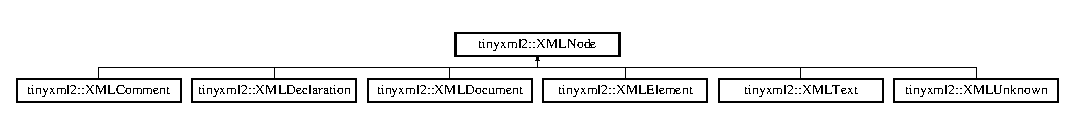
\includegraphics[height=1.145194cm]{classtinyxml2_1_1_x_m_l_node}
\end{center}
\end{figure}
\subsection*{Public Member Functions}
\begin{DoxyCompactItemize}
\item 
const \hyperlink{classtinyxml2_1_1_x_m_l_document}{X\+M\+L\+Document} $\ast$ \hyperlink{classtinyxml2_1_1_x_m_l_node_add244bca368083fa29698db8dcf147ca}{Get\+Document} () const 
\begin{DoxyCompactList}\small\item\em Get the \hyperlink{classtinyxml2_1_1_x_m_l_document}{X\+M\+L\+Document} that owns this \hyperlink{classtinyxml2_1_1_x_m_l_node}{X\+M\+L\+Node}. \end{DoxyCompactList}\item 
\hyperlink{classtinyxml2_1_1_x_m_l_document}{X\+M\+L\+Document} $\ast$ \hyperlink{classtinyxml2_1_1_x_m_l_node_af343d1ef0b45c0020e62d784d7e67a68}{Get\+Document} ()
\begin{DoxyCompactList}\small\item\em Get the \hyperlink{classtinyxml2_1_1_x_m_l_document}{X\+M\+L\+Document} that owns this \hyperlink{classtinyxml2_1_1_x_m_l_node}{X\+M\+L\+Node}. \end{DoxyCompactList}\item 
virtual \hyperlink{classtinyxml2_1_1_x_m_l_element}{X\+M\+L\+Element} $\ast$ \hyperlink{classtinyxml2_1_1_x_m_l_node_aab516e699567f75cc9ab2ef2eee501e8}{To\+Element} ()
\begin{DoxyCompactList}\small\item\em Safely cast to an Element, or null. \end{DoxyCompactList}\item 
virtual \hyperlink{classtinyxml2_1_1_x_m_l_text}{X\+M\+L\+Text} $\ast$ \hyperlink{classtinyxml2_1_1_x_m_l_node_a41c55dab9162d1eb62db2008430e376b}{To\+Text} ()
\begin{DoxyCompactList}\small\item\em Safely cast to Text, or null. \end{DoxyCompactList}\item 
virtual \hyperlink{classtinyxml2_1_1_x_m_l_comment}{X\+M\+L\+Comment} $\ast$ \hyperlink{classtinyxml2_1_1_x_m_l_node_aff47671055aa99840a1c1ebd661e63e3}{To\+Comment} ()
\begin{DoxyCompactList}\small\item\em Safely cast to a Comment, or null. \end{DoxyCompactList}\item 
virtual \hyperlink{classtinyxml2_1_1_x_m_l_document}{X\+M\+L\+Document} $\ast$ \hyperlink{classtinyxml2_1_1_x_m_l_node_a836e2966ed736fc3c94f70e12a2a3357}{To\+Document} ()
\begin{DoxyCompactList}\small\item\em Safely cast to a Document, or null. \end{DoxyCompactList}\item 
virtual \hyperlink{classtinyxml2_1_1_x_m_l_declaration}{X\+M\+L\+Declaration} $\ast$ \hyperlink{classtinyxml2_1_1_x_m_l_node_a174fd4c22c010b58138c1b84a0dfbd51}{To\+Declaration} ()
\begin{DoxyCompactList}\small\item\em Safely cast to a Declaration, or null. \end{DoxyCompactList}\item 
virtual \hyperlink{classtinyxml2_1_1_x_m_l_unknown}{X\+M\+L\+Unknown} $\ast$ \hyperlink{classtinyxml2_1_1_x_m_l_node_a8675a74aa0ada6eccab0c77ef3e5b9bd}{To\+Unknown} ()
\begin{DoxyCompactList}\small\item\em Safely cast to an Unknown, or null. \end{DoxyCompactList}\item 
virtual const \hyperlink{classtinyxml2_1_1_x_m_l_element}{X\+M\+L\+Element} $\ast$ \hyperlink{classtinyxml2_1_1_x_m_l_node_acbaec609797ddabb4f9dcf38ee91262e}{To\+Element} () const 
\item 
virtual const \hyperlink{classtinyxml2_1_1_x_m_l_text}{X\+M\+L\+Text} $\ast$ \hyperlink{classtinyxml2_1_1_x_m_l_node_a89009ffc1b9f5d692bf8d4c9f18c3bec}{To\+Text} () const 
\item 
virtual const \hyperlink{classtinyxml2_1_1_x_m_l_comment}{X\+M\+L\+Comment} $\ast$ \hyperlink{classtinyxml2_1_1_x_m_l_node_a157ce3a00ea5ee5a85b7103138e85e8a}{To\+Comment} () const 
\item 
virtual const \hyperlink{classtinyxml2_1_1_x_m_l_document}{X\+M\+L\+Document} $\ast$ \hyperlink{classtinyxml2_1_1_x_m_l_node_a3ff975733a17d6ced3539b45544c8bf6}{To\+Document} () const 
\item 
virtual const \hyperlink{classtinyxml2_1_1_x_m_l_declaration}{X\+M\+L\+Declaration} $\ast$ \hyperlink{classtinyxml2_1_1_x_m_l_node_aedae0bbb58d533a4b8a61042388b49e5}{To\+Declaration} () const 
\item 
virtual const \hyperlink{classtinyxml2_1_1_x_m_l_unknown}{X\+M\+L\+Unknown} $\ast$ \hyperlink{classtinyxml2_1_1_x_m_l_node_a71f5ae90296dbe67979f83fe97073efa}{To\+Unknown} () const 
\item 
const char $\ast$ \hyperlink{classtinyxml2_1_1_x_m_l_node_a92835c779871918f9af569bfe9669fe6}{Value} () const 
\item 
void \hyperlink{classtinyxml2_1_1_x_m_l_node_a09dd68cf9eae137579f6e50f36487513}{Set\+Value} (const char $\ast$val, bool static\+Mem=false)
\item 
const \hyperlink{classtinyxml2_1_1_x_m_l_node}{X\+M\+L\+Node} $\ast$ \hyperlink{classtinyxml2_1_1_x_m_l_node_a4e39bdcf9bfafa55d04857ece6aaf64e}{Parent} () const 
\begin{DoxyCompactList}\small\item\em Get the parent of this node on the D\+O\+M. \end{DoxyCompactList}\item 
\hyperlink{classtinyxml2_1_1_x_m_l_node}{X\+M\+L\+Node} $\ast$ \hyperlink{classtinyxml2_1_1_x_m_l_node_a76029693a5a54fbb721a41d7a0ca8a97}{Parent} ()
\item 
bool \hyperlink{classtinyxml2_1_1_x_m_l_node_a96afe34a9ccd0ed4c0cff32beb42cc6c}{No\+Children} () const 
\begin{DoxyCompactList}\small\item\em Returns true if this node has no children. \end{DoxyCompactList}\item 
const \hyperlink{classtinyxml2_1_1_x_m_l_node}{X\+M\+L\+Node} $\ast$ \hyperlink{classtinyxml2_1_1_x_m_l_node_a60e923d13d7dc01f45ab90a2f948b02a}{First\+Child} () const 
\begin{DoxyCompactList}\small\item\em Get the first child node, or null if none exists. \end{DoxyCompactList}\item 
\hyperlink{classtinyxml2_1_1_x_m_l_node}{X\+M\+L\+Node} $\ast$ \hyperlink{classtinyxml2_1_1_x_m_l_node_a2d6c70c475146b48bc93a7fafdeff5e0}{First\+Child} ()
\item 
const \hyperlink{classtinyxml2_1_1_x_m_l_element}{X\+M\+L\+Element} $\ast$ \hyperlink{classtinyxml2_1_1_x_m_l_node_a20f48e99b03e9c17487944f229bee130}{First\+Child\+Element} (const char $\ast$value=0) const 
\item 
\hyperlink{classtinyxml2_1_1_x_m_l_element}{X\+M\+L\+Element} $\ast$ \hyperlink{classtinyxml2_1_1_x_m_l_node_a7614c3b4eea1ff11b2aa90b0f92f6dba}{First\+Child\+Element} (const char $\ast$value=0)
\item 
const \hyperlink{classtinyxml2_1_1_x_m_l_node}{X\+M\+L\+Node} $\ast$ \hyperlink{classtinyxml2_1_1_x_m_l_node_a6088246532b02895beb0e6fa561a7f3b}{Last\+Child} () const 
\begin{DoxyCompactList}\small\item\em Get the last child node, or null if none exists. \end{DoxyCompactList}\item 
\hyperlink{classtinyxml2_1_1_x_m_l_node}{X\+M\+L\+Node} $\ast$ \hyperlink{classtinyxml2_1_1_x_m_l_node_ad7552c8cb1dc0cb6f3bdc14a9d115dbf}{Last\+Child} ()
\item 
const \hyperlink{classtinyxml2_1_1_x_m_l_element}{X\+M\+L\+Element} $\ast$ \hyperlink{classtinyxml2_1_1_x_m_l_node_a1a46cc01ece2216acf1e6294d1aff79d}{Last\+Child\+Element} (const char $\ast$value=0) const 
\item 
\hyperlink{classtinyxml2_1_1_x_m_l_element}{X\+M\+L\+Element} $\ast$ \hyperlink{classtinyxml2_1_1_x_m_l_node_a125423acf3170b130634638c5afc0639}{Last\+Child\+Element} (const char $\ast$value=0)
\item 
const \hyperlink{classtinyxml2_1_1_x_m_l_node}{X\+M\+L\+Node} $\ast$ \hyperlink{classtinyxml2_1_1_x_m_l_node_a4cb1bf63e9de55129d21a7be60685fd4}{Previous\+Sibling} () const 
\begin{DoxyCompactList}\small\item\em Get the previous (left) sibling node of this node. \end{DoxyCompactList}\item 
\hyperlink{classtinyxml2_1_1_x_m_l_node}{X\+M\+L\+Node} $\ast$ \hyperlink{classtinyxml2_1_1_x_m_l_node_ae760e5e7e766df1d2cf3bb4a847876d6}{Previous\+Sibling} ()
\item 
const \hyperlink{classtinyxml2_1_1_x_m_l_element}{X\+M\+L\+Element} $\ast$ \hyperlink{classtinyxml2_1_1_x_m_l_node_a573b2559c41dce244d893d610fbe0bd9}{Previous\+Sibling\+Element} (const char $\ast$value=0) const 
\begin{DoxyCompactList}\small\item\em Get the previous (left) sibling element of this node, with an optionally supplied name. \end{DoxyCompactList}\item 
\hyperlink{classtinyxml2_1_1_x_m_l_element}{X\+M\+L\+Element} $\ast$ \hyperlink{classtinyxml2_1_1_x_m_l_node_ae9177fdc49cb89879f333581d5f734f1}{Previous\+Sibling\+Element} (const char $\ast$value=0)
\item 
const \hyperlink{classtinyxml2_1_1_x_m_l_node}{X\+M\+L\+Node} $\ast$ \hyperlink{classtinyxml2_1_1_x_m_l_node_abba1df37581d89dccc45acdc55750ba2}{Next\+Sibling} () const 
\begin{DoxyCompactList}\small\item\em Get the next (right) sibling node of this node. \end{DoxyCompactList}\item 
\hyperlink{classtinyxml2_1_1_x_m_l_node}{X\+M\+L\+Node} $\ast$ \hyperlink{classtinyxml2_1_1_x_m_l_node_aeb7d4dfd8fb924ef86e7cb72183acbac}{Next\+Sibling} ()
\item 
const \hyperlink{classtinyxml2_1_1_x_m_l_element}{X\+M\+L\+Element} $\ast$ \hyperlink{classtinyxml2_1_1_x_m_l_node_a490e166c3a1c6607960bfa9c112d3d30}{Next\+Sibling\+Element} (const char $\ast$value=0) const 
\begin{DoxyCompactList}\small\item\em Get the next (right) sibling element of this node, with an optionally supplied name. \end{DoxyCompactList}\item 
\hyperlink{classtinyxml2_1_1_x_m_l_element}{X\+M\+L\+Element} $\ast$ \hyperlink{classtinyxml2_1_1_x_m_l_node_acf735bf653016792522305d8ad4b3029}{Next\+Sibling\+Element} (const char $\ast$value=0)
\item 
\hyperlink{classtinyxml2_1_1_x_m_l_node}{X\+M\+L\+Node} $\ast$ \hyperlink{classtinyxml2_1_1_x_m_l_node_ae3b422e98914d6002ca99bb1d2837103}{Insert\+End\+Child} (\hyperlink{classtinyxml2_1_1_x_m_l_node}{X\+M\+L\+Node} $\ast$add\+This)
\item 
\hyperlink{classtinyxml2_1_1_x_m_l_node}{X\+M\+L\+Node} $\ast$ \hyperlink{classtinyxml2_1_1_x_m_l_node_a663e3a5a378169fd477378f4d17a7649}{Link\+End\+Child} (\hyperlink{classtinyxml2_1_1_x_m_l_node}{X\+M\+L\+Node} $\ast$add\+This)
\item 
\hyperlink{classtinyxml2_1_1_x_m_l_node}{X\+M\+L\+Node} $\ast$ \hyperlink{classtinyxml2_1_1_x_m_l_node_ac609a8f3ea949027f439280c640bbaf2}{Insert\+First\+Child} (\hyperlink{classtinyxml2_1_1_x_m_l_node}{X\+M\+L\+Node} $\ast$add\+This)
\item 
\hyperlink{classtinyxml2_1_1_x_m_l_node}{X\+M\+L\+Node} $\ast$ \hyperlink{classtinyxml2_1_1_x_m_l_node_a9275138a1b8dd5d8e2c26789bdc23ac8}{Insert\+After\+Child} (\hyperlink{classtinyxml2_1_1_x_m_l_node}{X\+M\+L\+Node} $\ast$after\+This, \hyperlink{classtinyxml2_1_1_x_m_l_node}{X\+M\+L\+Node} $\ast$add\+This)
\item 
void \hyperlink{classtinyxml2_1_1_x_m_l_node_a0360085cc54df5bff85d5c5da13afdce}{Delete\+Children} ()
\item 
void \hyperlink{classtinyxml2_1_1_x_m_l_node_a363b6edbd6ebd55f8387d2b89f2b0921}{Delete\+Child} (\hyperlink{classtinyxml2_1_1_x_m_l_node}{X\+M\+L\+Node} $\ast$node)
\item 
virtual \hyperlink{classtinyxml2_1_1_x_m_l_node}{X\+M\+L\+Node} $\ast$ \hyperlink{classtinyxml2_1_1_x_m_l_node_a8402cbd3129d20e9e6024bbcc0531283}{Shallow\+Clone} (\hyperlink{classtinyxml2_1_1_x_m_l_document}{X\+M\+L\+Document} $\ast$document) const =0
\item 
virtual bool \hyperlink{classtinyxml2_1_1_x_m_l_node_a7ce18b751c3ea09eac292dca264f9226}{Shallow\+Equal} (const \hyperlink{classtinyxml2_1_1_x_m_l_node}{X\+M\+L\+Node} $\ast$compare) const =0
\item 
virtual bool \hyperlink{classtinyxml2_1_1_x_m_l_node_a81e66df0a44c67a7af17f3b77a152785}{Accept} (\hyperlink{classtinyxml2_1_1_x_m_l_visitor}{X\+M\+L\+Visitor} $\ast$visitor) const =0
\item 
virtual char $\ast$ \hyperlink{classtinyxml2_1_1_x_m_l_node_a7610d0f603e8b603d2078521811a23c1}{Parse\+Deep} (char $\ast$, \hyperlink{classtinyxml2_1_1_str_pair}{Str\+Pair} $\ast$)
\end{DoxyCompactItemize}
\subsection*{Protected Member Functions}
\begin{DoxyCompactItemize}
\item 
\hyperlink{classtinyxml2_1_1_x_m_l_node_a29868df6ca383d574f584dfdd15105b6}{X\+M\+L\+Node} (\hyperlink{classtinyxml2_1_1_x_m_l_document}{X\+M\+L\+Document} $\ast$)
\item 
virtual \hyperlink{classtinyxml2_1_1_x_m_l_node_a8f41e898cdd4da4cdbb7f05b0c7d9f69}{$\sim$\+X\+M\+L\+Node} ()
\end{DoxyCompactItemize}
\subsection*{Protected Attributes}
\begin{DoxyCompactItemize}
\item 
\hyperlink{classtinyxml2_1_1_x_m_l_document}{X\+M\+L\+Document} $\ast$ \hyperlink{classtinyxml2_1_1_x_m_l_node_a8d2d2be0bb6797625551eb0e91f0ff62}{\+\_\+document}
\item 
\hyperlink{classtinyxml2_1_1_x_m_l_node}{X\+M\+L\+Node} $\ast$ \hyperlink{classtinyxml2_1_1_x_m_l_node_a176dd1c4965c21c366de192164aa2c13}{\+\_\+parent}
\item 
\hyperlink{classtinyxml2_1_1_str_pair}{Str\+Pair} \hyperlink{classtinyxml2_1_1_x_m_l_node_a3ea9884098b8379de2bb5ab3fc85c0fc}{\+\_\+value}
\item 
\hyperlink{classtinyxml2_1_1_x_m_l_node}{X\+M\+L\+Node} $\ast$ \hyperlink{classtinyxml2_1_1_x_m_l_node_aa20c91e4213dc930c5bdf420322ca342}{\+\_\+first\+Child}
\item 
\hyperlink{classtinyxml2_1_1_x_m_l_node}{X\+M\+L\+Node} $\ast$ \hyperlink{classtinyxml2_1_1_x_m_l_node_a099b6560ae44ab9edb8453aaf1a3747b}{\+\_\+last\+Child}
\item 
\hyperlink{classtinyxml2_1_1_x_m_l_node}{X\+M\+L\+Node} $\ast$ \hyperlink{classtinyxml2_1_1_x_m_l_node_a9739eb0fb9a1188266052055e7a6bf6b}{\+\_\+prev}
\item 
\hyperlink{classtinyxml2_1_1_x_m_l_node}{X\+M\+L\+Node} $\ast$ \hyperlink{classtinyxml2_1_1_x_m_l_node_a27e985496b37dd00eb5b9cf59b9e3fb1}{\+\_\+next}
\end{DoxyCompactItemize}
\subsection*{Friends}
\begin{DoxyCompactItemize}
\item 
class \hyperlink{classtinyxml2_1_1_x_m_l_node_a4eee3bda60c60a30e4e8cd4ea91c4c6e}{X\+M\+L\+Document}
\item 
class \hyperlink{classtinyxml2_1_1_x_m_l_node_ac2fba9b6e452829dd892f7392c24e0eb}{X\+M\+L\+Element}
\end{DoxyCompactItemize}


\subsection{Detailed Description}
\hyperlink{classtinyxml2_1_1_x_m_l_node}{X\+M\+L\+Node} is a base class for every object that is in the X\+M\+L Document Object Model (D\+O\+M), except X\+M\+L\+Attributes. Nodes have siblings, a parent, and children which can be navigated. A node is always in a \hyperlink{classtinyxml2_1_1_x_m_l_document}{X\+M\+L\+Document}. The type of a \hyperlink{classtinyxml2_1_1_x_m_l_node}{X\+M\+L\+Node} can be queried, and it can be cast to its more defined type.

A \hyperlink{classtinyxml2_1_1_x_m_l_document}{X\+M\+L\+Document} allocates memory for all its Nodes. When the \hyperlink{classtinyxml2_1_1_x_m_l_document}{X\+M\+L\+Document} gets deleted, all its Nodes will also be deleted.

\begin{DoxyVerb}A Document can contain: Element (container or leaf)
                        Comment (leaf)
                        Unknown (leaf)
                        Declaration( leaf )

An Element can contain: Element (container or leaf)
                        Text    (leaf)
                        Attributes (not on tree)
                        Comment (leaf)
                        Unknown (leaf)\end{DoxyVerb}
 

\subsection{Constructor \& Destructor Documentation}
\hypertarget{classtinyxml2_1_1_x_m_l_node_a29868df6ca383d574f584dfdd15105b6}{}\index{tinyxml2\+::\+X\+M\+L\+Node@{tinyxml2\+::\+X\+M\+L\+Node}!X\+M\+L\+Node@{X\+M\+L\+Node}}
\index{X\+M\+L\+Node@{X\+M\+L\+Node}!tinyxml2\+::\+X\+M\+L\+Node@{tinyxml2\+::\+X\+M\+L\+Node}}
\subsubsection[{X\+M\+L\+Node}]{\setlength{\rightskip}{0pt plus 5cm}tinyxml2\+::\+X\+M\+L\+Node\+::\+X\+M\+L\+Node (
\begin{DoxyParamCaption}
\item[{{\bf X\+M\+L\+Document} $\ast$}]{doc}
\end{DoxyParamCaption}
)\hspace{0.3cm}{\ttfamily [protected]}}\label{classtinyxml2_1_1_x_m_l_node_a29868df6ca383d574f584dfdd15105b6}
\hypertarget{classtinyxml2_1_1_x_m_l_node_a8f41e898cdd4da4cdbb7f05b0c7d9f69}{}\index{tinyxml2\+::\+X\+M\+L\+Node@{tinyxml2\+::\+X\+M\+L\+Node}!````~X\+M\+L\+Node@{$\sim$\+X\+M\+L\+Node}}
\index{````~X\+M\+L\+Node@{$\sim$\+X\+M\+L\+Node}!tinyxml2\+::\+X\+M\+L\+Node@{tinyxml2\+::\+X\+M\+L\+Node}}
\subsubsection[{$\sim$\+X\+M\+L\+Node}]{\setlength{\rightskip}{0pt plus 5cm}tinyxml2\+::\+X\+M\+L\+Node\+::$\sim$\+X\+M\+L\+Node (
\begin{DoxyParamCaption}
{}
\end{DoxyParamCaption}
)\hspace{0.3cm}{\ttfamily [protected]}, {\ttfamily [virtual]}}\label{classtinyxml2_1_1_x_m_l_node_a8f41e898cdd4da4cdbb7f05b0c7d9f69}


\subsection{Member Function Documentation}
\hypertarget{classtinyxml2_1_1_x_m_l_node_a81e66df0a44c67a7af17f3b77a152785}{}\index{tinyxml2\+::\+X\+M\+L\+Node@{tinyxml2\+::\+X\+M\+L\+Node}!Accept@{Accept}}
\index{Accept@{Accept}!tinyxml2\+::\+X\+M\+L\+Node@{tinyxml2\+::\+X\+M\+L\+Node}}
\subsubsection[{Accept}]{\setlength{\rightskip}{0pt plus 5cm}virtual bool tinyxml2\+::\+X\+M\+L\+Node\+::\+Accept (
\begin{DoxyParamCaption}
\item[{{\bf X\+M\+L\+Visitor} $\ast$}]{visitor}
\end{DoxyParamCaption}
) const\hspace{0.3cm}{\ttfamily [pure virtual]}}\label{classtinyxml2_1_1_x_m_l_node_a81e66df0a44c67a7af17f3b77a152785}
Accept a hierarchical visit of the nodes in the Tiny\+X\+M\+L-\/2 D\+O\+M. Every node in the X\+M\+L tree will be conditionally visited and the host will be called back via the \hyperlink{classtinyxml2_1_1_x_m_l_visitor}{X\+M\+L\+Visitor} interface.

This is essentially a S\+A\+X interface for Tiny\+X\+M\+L-\/2. (Note however it doesn\textquotesingle{}t re-\/parse the X\+M\+L for the callbacks, so the performance of Tiny\+X\+M\+L-\/2 is unchanged by using this interface versus any other.)

The interface has been based on ideas from\+:


\begin{DoxyItemize}
\item \href{http://www.saxproject.org/}{\tt http\+://www.\+saxproject.\+org/}
\item \href{http://c2.com/cgi/wiki?HierarchicalVisitorPattern}{\tt http\+://c2.\+com/cgi/wiki?\+Hierarchical\+Visitor\+Pattern}
\end{DoxyItemize}

Which are both good references for \char`\"{}visiting\char`\"{}.

An example of using \hyperlink{classtinyxml2_1_1_x_m_l_node_a81e66df0a44c67a7af17f3b77a152785}{Accept()}\+: \begin{DoxyVerb}XMLPrinter printer;
tinyxmlDoc.Accept( &printer );
const char* xmlcstr = printer.CStr();
\end{DoxyVerb}
 

Implemented in \hyperlink{classtinyxml2_1_1_x_m_l_document_aa08503d24898bf9992ae5e5fb8b0cf87}{tinyxml2\+::\+X\+M\+L\+Document}, \hyperlink{classtinyxml2_1_1_x_m_l_element_a36d65438991a1e85096caf39ad13a099}{tinyxml2\+::\+X\+M\+L\+Element}, \hyperlink{classtinyxml2_1_1_x_m_l_unknown_a0d341ab804a1438a474810bb5bd29dd5}{tinyxml2\+::\+X\+M\+L\+Unknown}, \hyperlink{classtinyxml2_1_1_x_m_l_declaration_a953a7359cc312d15218eb5843a4ca108}{tinyxml2\+::\+X\+M\+L\+Declaration}, \hyperlink{classtinyxml2_1_1_x_m_l_comment_aa382b1be6a8b0650c16a2d88bb499335}{tinyxml2\+::\+X\+M\+L\+Comment}, and \hyperlink{classtinyxml2_1_1_x_m_l_text_ae659d4fc7351a7df11c111cbe1ade46f}{tinyxml2\+::\+X\+M\+L\+Text}.

\hypertarget{classtinyxml2_1_1_x_m_l_node_a363b6edbd6ebd55f8387d2b89f2b0921}{}\index{tinyxml2\+::\+X\+M\+L\+Node@{tinyxml2\+::\+X\+M\+L\+Node}!Delete\+Child@{Delete\+Child}}
\index{Delete\+Child@{Delete\+Child}!tinyxml2\+::\+X\+M\+L\+Node@{tinyxml2\+::\+X\+M\+L\+Node}}
\subsubsection[{Delete\+Child}]{\setlength{\rightskip}{0pt plus 5cm}void tinyxml2\+::\+X\+M\+L\+Node\+::\+Delete\+Child (
\begin{DoxyParamCaption}
\item[{{\bf X\+M\+L\+Node} $\ast$}]{node}
\end{DoxyParamCaption}
)}\label{classtinyxml2_1_1_x_m_l_node_a363b6edbd6ebd55f8387d2b89f2b0921}
Delete a child of this node. \hypertarget{classtinyxml2_1_1_x_m_l_node_a0360085cc54df5bff85d5c5da13afdce}{}\index{tinyxml2\+::\+X\+M\+L\+Node@{tinyxml2\+::\+X\+M\+L\+Node}!Delete\+Children@{Delete\+Children}}
\index{Delete\+Children@{Delete\+Children}!tinyxml2\+::\+X\+M\+L\+Node@{tinyxml2\+::\+X\+M\+L\+Node}}
\subsubsection[{Delete\+Children}]{\setlength{\rightskip}{0pt plus 5cm}void tinyxml2\+::\+X\+M\+L\+Node\+::\+Delete\+Children (
\begin{DoxyParamCaption}
{}
\end{DoxyParamCaption}
)}\label{classtinyxml2_1_1_x_m_l_node_a0360085cc54df5bff85d5c5da13afdce}
Delete all the children of this node. \hypertarget{classtinyxml2_1_1_x_m_l_node_a60e923d13d7dc01f45ab90a2f948b02a}{}\index{tinyxml2\+::\+X\+M\+L\+Node@{tinyxml2\+::\+X\+M\+L\+Node}!First\+Child@{First\+Child}}
\index{First\+Child@{First\+Child}!tinyxml2\+::\+X\+M\+L\+Node@{tinyxml2\+::\+X\+M\+L\+Node}}
\subsubsection[{First\+Child}]{\setlength{\rightskip}{0pt plus 5cm}const {\bf X\+M\+L\+Node}$\ast$ tinyxml2\+::\+X\+M\+L\+Node\+::\+First\+Child (
\begin{DoxyParamCaption}
{}
\end{DoxyParamCaption}
) const\hspace{0.3cm}{\ttfamily [inline]}}\label{classtinyxml2_1_1_x_m_l_node_a60e923d13d7dc01f45ab90a2f948b02a}


Get the first child node, or null if none exists. 

\hypertarget{classtinyxml2_1_1_x_m_l_node_a2d6c70c475146b48bc93a7fafdeff5e0}{}\index{tinyxml2\+::\+X\+M\+L\+Node@{tinyxml2\+::\+X\+M\+L\+Node}!First\+Child@{First\+Child}}
\index{First\+Child@{First\+Child}!tinyxml2\+::\+X\+M\+L\+Node@{tinyxml2\+::\+X\+M\+L\+Node}}
\subsubsection[{First\+Child}]{\setlength{\rightskip}{0pt plus 5cm}{\bf X\+M\+L\+Node}$\ast$ tinyxml2\+::\+X\+M\+L\+Node\+::\+First\+Child (
\begin{DoxyParamCaption}
{}
\end{DoxyParamCaption}
)\hspace{0.3cm}{\ttfamily [inline]}}\label{classtinyxml2_1_1_x_m_l_node_a2d6c70c475146b48bc93a7fafdeff5e0}
\hypertarget{classtinyxml2_1_1_x_m_l_node_a20f48e99b03e9c17487944f229bee130}{}\index{tinyxml2\+::\+X\+M\+L\+Node@{tinyxml2\+::\+X\+M\+L\+Node}!First\+Child\+Element@{First\+Child\+Element}}
\index{First\+Child\+Element@{First\+Child\+Element}!tinyxml2\+::\+X\+M\+L\+Node@{tinyxml2\+::\+X\+M\+L\+Node}}
\subsubsection[{First\+Child\+Element}]{\setlength{\rightskip}{0pt plus 5cm}const {\bf X\+M\+L\+Element} $\ast$ tinyxml2\+::\+X\+M\+L\+Node\+::\+First\+Child\+Element (
\begin{DoxyParamCaption}
\item[{const char $\ast$}]{value = {\ttfamily 0}}
\end{DoxyParamCaption}
) const}\label{classtinyxml2_1_1_x_m_l_node_a20f48e99b03e9c17487944f229bee130}
Get the first child element, or optionally the first child element with the specified name. \hypertarget{classtinyxml2_1_1_x_m_l_node_a7614c3b4eea1ff11b2aa90b0f92f6dba}{}\index{tinyxml2\+::\+X\+M\+L\+Node@{tinyxml2\+::\+X\+M\+L\+Node}!First\+Child\+Element@{First\+Child\+Element}}
\index{First\+Child\+Element@{First\+Child\+Element}!tinyxml2\+::\+X\+M\+L\+Node@{tinyxml2\+::\+X\+M\+L\+Node}}
\subsubsection[{First\+Child\+Element}]{\setlength{\rightskip}{0pt plus 5cm}{\bf X\+M\+L\+Element}$\ast$ tinyxml2\+::\+X\+M\+L\+Node\+::\+First\+Child\+Element (
\begin{DoxyParamCaption}
\item[{const char $\ast$}]{value = {\ttfamily 0}}
\end{DoxyParamCaption}
)\hspace{0.3cm}{\ttfamily [inline]}}\label{classtinyxml2_1_1_x_m_l_node_a7614c3b4eea1ff11b2aa90b0f92f6dba}
\hypertarget{classtinyxml2_1_1_x_m_l_node_add244bca368083fa29698db8dcf147ca}{}\index{tinyxml2\+::\+X\+M\+L\+Node@{tinyxml2\+::\+X\+M\+L\+Node}!Get\+Document@{Get\+Document}}
\index{Get\+Document@{Get\+Document}!tinyxml2\+::\+X\+M\+L\+Node@{tinyxml2\+::\+X\+M\+L\+Node}}
\subsubsection[{Get\+Document}]{\setlength{\rightskip}{0pt plus 5cm}const {\bf X\+M\+L\+Document}$\ast$ tinyxml2\+::\+X\+M\+L\+Node\+::\+Get\+Document (
\begin{DoxyParamCaption}
{}
\end{DoxyParamCaption}
) const\hspace{0.3cm}{\ttfamily [inline]}}\label{classtinyxml2_1_1_x_m_l_node_add244bca368083fa29698db8dcf147ca}


Get the \hyperlink{classtinyxml2_1_1_x_m_l_document}{X\+M\+L\+Document} that owns this \hyperlink{classtinyxml2_1_1_x_m_l_node}{X\+M\+L\+Node}. 

\hypertarget{classtinyxml2_1_1_x_m_l_node_af343d1ef0b45c0020e62d784d7e67a68}{}\index{tinyxml2\+::\+X\+M\+L\+Node@{tinyxml2\+::\+X\+M\+L\+Node}!Get\+Document@{Get\+Document}}
\index{Get\+Document@{Get\+Document}!tinyxml2\+::\+X\+M\+L\+Node@{tinyxml2\+::\+X\+M\+L\+Node}}
\subsubsection[{Get\+Document}]{\setlength{\rightskip}{0pt plus 5cm}{\bf X\+M\+L\+Document}$\ast$ tinyxml2\+::\+X\+M\+L\+Node\+::\+Get\+Document (
\begin{DoxyParamCaption}
{}
\end{DoxyParamCaption}
)\hspace{0.3cm}{\ttfamily [inline]}}\label{classtinyxml2_1_1_x_m_l_node_af343d1ef0b45c0020e62d784d7e67a68}


Get the \hyperlink{classtinyxml2_1_1_x_m_l_document}{X\+M\+L\+Document} that owns this \hyperlink{classtinyxml2_1_1_x_m_l_node}{X\+M\+L\+Node}. 

\hypertarget{classtinyxml2_1_1_x_m_l_node_a9275138a1b8dd5d8e2c26789bdc23ac8}{}\index{tinyxml2\+::\+X\+M\+L\+Node@{tinyxml2\+::\+X\+M\+L\+Node}!Insert\+After\+Child@{Insert\+After\+Child}}
\index{Insert\+After\+Child@{Insert\+After\+Child}!tinyxml2\+::\+X\+M\+L\+Node@{tinyxml2\+::\+X\+M\+L\+Node}}
\subsubsection[{Insert\+After\+Child}]{\setlength{\rightskip}{0pt plus 5cm}{\bf X\+M\+L\+Node} $\ast$ tinyxml2\+::\+X\+M\+L\+Node\+::\+Insert\+After\+Child (
\begin{DoxyParamCaption}
\item[{{\bf X\+M\+L\+Node} $\ast$}]{after\+This, }
\item[{{\bf X\+M\+L\+Node} $\ast$}]{add\+This}
\end{DoxyParamCaption}
)}\label{classtinyxml2_1_1_x_m_l_node_a9275138a1b8dd5d8e2c26789bdc23ac8}
Add a node after the specified child node. If the child node is already part of the document, it is moved from its old location to the new location. Returns the add\+This argument or 0 if the after\+This node is not a child of this node, or if the node does not belong to the same document. \hypertarget{classtinyxml2_1_1_x_m_l_node_ae3b422e98914d6002ca99bb1d2837103}{}\index{tinyxml2\+::\+X\+M\+L\+Node@{tinyxml2\+::\+X\+M\+L\+Node}!Insert\+End\+Child@{Insert\+End\+Child}}
\index{Insert\+End\+Child@{Insert\+End\+Child}!tinyxml2\+::\+X\+M\+L\+Node@{tinyxml2\+::\+X\+M\+L\+Node}}
\subsubsection[{Insert\+End\+Child}]{\setlength{\rightskip}{0pt plus 5cm}{\bf X\+M\+L\+Node} $\ast$ tinyxml2\+::\+X\+M\+L\+Node\+::\+Insert\+End\+Child (
\begin{DoxyParamCaption}
\item[{{\bf X\+M\+L\+Node} $\ast$}]{add\+This}
\end{DoxyParamCaption}
)}\label{classtinyxml2_1_1_x_m_l_node_ae3b422e98914d6002ca99bb1d2837103}
Add a child node as the last (right) child. If the child node is already part of the document, it is moved from its old location to the new location. Returns the add\+This argument or 0 if the node does not belong to the same document. \hypertarget{classtinyxml2_1_1_x_m_l_node_ac609a8f3ea949027f439280c640bbaf2}{}\index{tinyxml2\+::\+X\+M\+L\+Node@{tinyxml2\+::\+X\+M\+L\+Node}!Insert\+First\+Child@{Insert\+First\+Child}}
\index{Insert\+First\+Child@{Insert\+First\+Child}!tinyxml2\+::\+X\+M\+L\+Node@{tinyxml2\+::\+X\+M\+L\+Node}}
\subsubsection[{Insert\+First\+Child}]{\setlength{\rightskip}{0pt plus 5cm}{\bf X\+M\+L\+Node} $\ast$ tinyxml2\+::\+X\+M\+L\+Node\+::\+Insert\+First\+Child (
\begin{DoxyParamCaption}
\item[{{\bf X\+M\+L\+Node} $\ast$}]{add\+This}
\end{DoxyParamCaption}
)}\label{classtinyxml2_1_1_x_m_l_node_ac609a8f3ea949027f439280c640bbaf2}
Add a child node as the first (left) child. If the child node is already part of the document, it is moved from its old location to the new location. Returns the add\+This argument or 0 if the node does not belong to the same document. \hypertarget{classtinyxml2_1_1_x_m_l_node_a6088246532b02895beb0e6fa561a7f3b}{}\index{tinyxml2\+::\+X\+M\+L\+Node@{tinyxml2\+::\+X\+M\+L\+Node}!Last\+Child@{Last\+Child}}
\index{Last\+Child@{Last\+Child}!tinyxml2\+::\+X\+M\+L\+Node@{tinyxml2\+::\+X\+M\+L\+Node}}
\subsubsection[{Last\+Child}]{\setlength{\rightskip}{0pt plus 5cm}const {\bf X\+M\+L\+Node}$\ast$ tinyxml2\+::\+X\+M\+L\+Node\+::\+Last\+Child (
\begin{DoxyParamCaption}
{}
\end{DoxyParamCaption}
) const\hspace{0.3cm}{\ttfamily [inline]}}\label{classtinyxml2_1_1_x_m_l_node_a6088246532b02895beb0e6fa561a7f3b}


Get the last child node, or null if none exists. 

\hypertarget{classtinyxml2_1_1_x_m_l_node_ad7552c8cb1dc0cb6f3bdc14a9d115dbf}{}\index{tinyxml2\+::\+X\+M\+L\+Node@{tinyxml2\+::\+X\+M\+L\+Node}!Last\+Child@{Last\+Child}}
\index{Last\+Child@{Last\+Child}!tinyxml2\+::\+X\+M\+L\+Node@{tinyxml2\+::\+X\+M\+L\+Node}}
\subsubsection[{Last\+Child}]{\setlength{\rightskip}{0pt plus 5cm}{\bf X\+M\+L\+Node}$\ast$ tinyxml2\+::\+X\+M\+L\+Node\+::\+Last\+Child (
\begin{DoxyParamCaption}
{}
\end{DoxyParamCaption}
)\hspace{0.3cm}{\ttfamily [inline]}}\label{classtinyxml2_1_1_x_m_l_node_ad7552c8cb1dc0cb6f3bdc14a9d115dbf}
\hypertarget{classtinyxml2_1_1_x_m_l_node_a1a46cc01ece2216acf1e6294d1aff79d}{}\index{tinyxml2\+::\+X\+M\+L\+Node@{tinyxml2\+::\+X\+M\+L\+Node}!Last\+Child\+Element@{Last\+Child\+Element}}
\index{Last\+Child\+Element@{Last\+Child\+Element}!tinyxml2\+::\+X\+M\+L\+Node@{tinyxml2\+::\+X\+M\+L\+Node}}
\subsubsection[{Last\+Child\+Element}]{\setlength{\rightskip}{0pt plus 5cm}const {\bf X\+M\+L\+Element} $\ast$ tinyxml2\+::\+X\+M\+L\+Node\+::\+Last\+Child\+Element (
\begin{DoxyParamCaption}
\item[{const char $\ast$}]{value = {\ttfamily 0}}
\end{DoxyParamCaption}
) const}\label{classtinyxml2_1_1_x_m_l_node_a1a46cc01ece2216acf1e6294d1aff79d}
Get the last child element or optionally the last child element with the specified name. \hypertarget{classtinyxml2_1_1_x_m_l_node_a125423acf3170b130634638c5afc0639}{}\index{tinyxml2\+::\+X\+M\+L\+Node@{tinyxml2\+::\+X\+M\+L\+Node}!Last\+Child\+Element@{Last\+Child\+Element}}
\index{Last\+Child\+Element@{Last\+Child\+Element}!tinyxml2\+::\+X\+M\+L\+Node@{tinyxml2\+::\+X\+M\+L\+Node}}
\subsubsection[{Last\+Child\+Element}]{\setlength{\rightskip}{0pt plus 5cm}{\bf X\+M\+L\+Element}$\ast$ tinyxml2\+::\+X\+M\+L\+Node\+::\+Last\+Child\+Element (
\begin{DoxyParamCaption}
\item[{const char $\ast$}]{value = {\ttfamily 0}}
\end{DoxyParamCaption}
)\hspace{0.3cm}{\ttfamily [inline]}}\label{classtinyxml2_1_1_x_m_l_node_a125423acf3170b130634638c5afc0639}
\hypertarget{classtinyxml2_1_1_x_m_l_node_a663e3a5a378169fd477378f4d17a7649}{}\index{tinyxml2\+::\+X\+M\+L\+Node@{tinyxml2\+::\+X\+M\+L\+Node}!Link\+End\+Child@{Link\+End\+Child}}
\index{Link\+End\+Child@{Link\+End\+Child}!tinyxml2\+::\+X\+M\+L\+Node@{tinyxml2\+::\+X\+M\+L\+Node}}
\subsubsection[{Link\+End\+Child}]{\setlength{\rightskip}{0pt plus 5cm}{\bf X\+M\+L\+Node}$\ast$ tinyxml2\+::\+X\+M\+L\+Node\+::\+Link\+End\+Child (
\begin{DoxyParamCaption}
\item[{{\bf X\+M\+L\+Node} $\ast$}]{add\+This}
\end{DoxyParamCaption}
)\hspace{0.3cm}{\ttfamily [inline]}}\label{classtinyxml2_1_1_x_m_l_node_a663e3a5a378169fd477378f4d17a7649}
\hypertarget{classtinyxml2_1_1_x_m_l_node_abba1df37581d89dccc45acdc55750ba2}{}\index{tinyxml2\+::\+X\+M\+L\+Node@{tinyxml2\+::\+X\+M\+L\+Node}!Next\+Sibling@{Next\+Sibling}}
\index{Next\+Sibling@{Next\+Sibling}!tinyxml2\+::\+X\+M\+L\+Node@{tinyxml2\+::\+X\+M\+L\+Node}}
\subsubsection[{Next\+Sibling}]{\setlength{\rightskip}{0pt plus 5cm}const {\bf X\+M\+L\+Node}$\ast$ tinyxml2\+::\+X\+M\+L\+Node\+::\+Next\+Sibling (
\begin{DoxyParamCaption}
{}
\end{DoxyParamCaption}
) const\hspace{0.3cm}{\ttfamily [inline]}}\label{classtinyxml2_1_1_x_m_l_node_abba1df37581d89dccc45acdc55750ba2}


Get the next (right) sibling node of this node. 

\hypertarget{classtinyxml2_1_1_x_m_l_node_aeb7d4dfd8fb924ef86e7cb72183acbac}{}\index{tinyxml2\+::\+X\+M\+L\+Node@{tinyxml2\+::\+X\+M\+L\+Node}!Next\+Sibling@{Next\+Sibling}}
\index{Next\+Sibling@{Next\+Sibling}!tinyxml2\+::\+X\+M\+L\+Node@{tinyxml2\+::\+X\+M\+L\+Node}}
\subsubsection[{Next\+Sibling}]{\setlength{\rightskip}{0pt plus 5cm}{\bf X\+M\+L\+Node}$\ast$ tinyxml2\+::\+X\+M\+L\+Node\+::\+Next\+Sibling (
\begin{DoxyParamCaption}
{}
\end{DoxyParamCaption}
)\hspace{0.3cm}{\ttfamily [inline]}}\label{classtinyxml2_1_1_x_m_l_node_aeb7d4dfd8fb924ef86e7cb72183acbac}
\hypertarget{classtinyxml2_1_1_x_m_l_node_a490e166c3a1c6607960bfa9c112d3d30}{}\index{tinyxml2\+::\+X\+M\+L\+Node@{tinyxml2\+::\+X\+M\+L\+Node}!Next\+Sibling\+Element@{Next\+Sibling\+Element}}
\index{Next\+Sibling\+Element@{Next\+Sibling\+Element}!tinyxml2\+::\+X\+M\+L\+Node@{tinyxml2\+::\+X\+M\+L\+Node}}
\subsubsection[{Next\+Sibling\+Element}]{\setlength{\rightskip}{0pt plus 5cm}const {\bf X\+M\+L\+Element} $\ast$ tinyxml2\+::\+X\+M\+L\+Node\+::\+Next\+Sibling\+Element (
\begin{DoxyParamCaption}
\item[{const char $\ast$}]{value = {\ttfamily 0}}
\end{DoxyParamCaption}
) const}\label{classtinyxml2_1_1_x_m_l_node_a490e166c3a1c6607960bfa9c112d3d30}


Get the next (right) sibling element of this node, with an optionally supplied name. 

\hypertarget{classtinyxml2_1_1_x_m_l_node_acf735bf653016792522305d8ad4b3029}{}\index{tinyxml2\+::\+X\+M\+L\+Node@{tinyxml2\+::\+X\+M\+L\+Node}!Next\+Sibling\+Element@{Next\+Sibling\+Element}}
\index{Next\+Sibling\+Element@{Next\+Sibling\+Element}!tinyxml2\+::\+X\+M\+L\+Node@{tinyxml2\+::\+X\+M\+L\+Node}}
\subsubsection[{Next\+Sibling\+Element}]{\setlength{\rightskip}{0pt plus 5cm}{\bf X\+M\+L\+Element}$\ast$ tinyxml2\+::\+X\+M\+L\+Node\+::\+Next\+Sibling\+Element (
\begin{DoxyParamCaption}
\item[{const char $\ast$}]{value = {\ttfamily 0}}
\end{DoxyParamCaption}
)\hspace{0.3cm}{\ttfamily [inline]}}\label{classtinyxml2_1_1_x_m_l_node_acf735bf653016792522305d8ad4b3029}
\hypertarget{classtinyxml2_1_1_x_m_l_node_a96afe34a9ccd0ed4c0cff32beb42cc6c}{}\index{tinyxml2\+::\+X\+M\+L\+Node@{tinyxml2\+::\+X\+M\+L\+Node}!No\+Children@{No\+Children}}
\index{No\+Children@{No\+Children}!tinyxml2\+::\+X\+M\+L\+Node@{tinyxml2\+::\+X\+M\+L\+Node}}
\subsubsection[{No\+Children}]{\setlength{\rightskip}{0pt plus 5cm}bool tinyxml2\+::\+X\+M\+L\+Node\+::\+No\+Children (
\begin{DoxyParamCaption}
{}
\end{DoxyParamCaption}
) const\hspace{0.3cm}{\ttfamily [inline]}}\label{classtinyxml2_1_1_x_m_l_node_a96afe34a9ccd0ed4c0cff32beb42cc6c}


Returns true if this node has no children. 

\hypertarget{classtinyxml2_1_1_x_m_l_node_a4e39bdcf9bfafa55d04857ece6aaf64e}{}\index{tinyxml2\+::\+X\+M\+L\+Node@{tinyxml2\+::\+X\+M\+L\+Node}!Parent@{Parent}}
\index{Parent@{Parent}!tinyxml2\+::\+X\+M\+L\+Node@{tinyxml2\+::\+X\+M\+L\+Node}}
\subsubsection[{Parent}]{\setlength{\rightskip}{0pt plus 5cm}const {\bf X\+M\+L\+Node}$\ast$ tinyxml2\+::\+X\+M\+L\+Node\+::\+Parent (
\begin{DoxyParamCaption}
{}
\end{DoxyParamCaption}
) const\hspace{0.3cm}{\ttfamily [inline]}}\label{classtinyxml2_1_1_x_m_l_node_a4e39bdcf9bfafa55d04857ece6aaf64e}


Get the parent of this node on the D\+O\+M. 

\hypertarget{classtinyxml2_1_1_x_m_l_node_a76029693a5a54fbb721a41d7a0ca8a97}{}\index{tinyxml2\+::\+X\+M\+L\+Node@{tinyxml2\+::\+X\+M\+L\+Node}!Parent@{Parent}}
\index{Parent@{Parent}!tinyxml2\+::\+X\+M\+L\+Node@{tinyxml2\+::\+X\+M\+L\+Node}}
\subsubsection[{Parent}]{\setlength{\rightskip}{0pt plus 5cm}{\bf X\+M\+L\+Node}$\ast$ tinyxml2\+::\+X\+M\+L\+Node\+::\+Parent (
\begin{DoxyParamCaption}
{}
\end{DoxyParamCaption}
)\hspace{0.3cm}{\ttfamily [inline]}}\label{classtinyxml2_1_1_x_m_l_node_a76029693a5a54fbb721a41d7a0ca8a97}
\hypertarget{classtinyxml2_1_1_x_m_l_node_a7610d0f603e8b603d2078521811a23c1}{}\index{tinyxml2\+::\+X\+M\+L\+Node@{tinyxml2\+::\+X\+M\+L\+Node}!Parse\+Deep@{Parse\+Deep}}
\index{Parse\+Deep@{Parse\+Deep}!tinyxml2\+::\+X\+M\+L\+Node@{tinyxml2\+::\+X\+M\+L\+Node}}
\subsubsection[{Parse\+Deep}]{\setlength{\rightskip}{0pt plus 5cm}char $\ast$ tinyxml2\+::\+X\+M\+L\+Node\+::\+Parse\+Deep (
\begin{DoxyParamCaption}
\item[{char $\ast$}]{p, }
\item[{{\bf Str\+Pair} $\ast$}]{parent\+End}
\end{DoxyParamCaption}
)\hspace{0.3cm}{\ttfamily [virtual]}}\label{classtinyxml2_1_1_x_m_l_node_a7610d0f603e8b603d2078521811a23c1}


Reimplemented in \hyperlink{classtinyxml2_1_1_x_m_l_element_aaafdd2a5618abe80a2c1839ad3ccd492}{tinyxml2\+::\+X\+M\+L\+Element}, \hyperlink{classtinyxml2_1_1_x_m_l_unknown_a0e4f3509dee42a4d45a7f0002be568cc}{tinyxml2\+::\+X\+M\+L\+Unknown}, \hyperlink{classtinyxml2_1_1_x_m_l_declaration_a19e33e0a9f9500f449261558c36f9a44}{tinyxml2\+::\+X\+M\+L\+Declaration}, \hyperlink{classtinyxml2_1_1_x_m_l_comment_aa6ab35c3bb1c1840371dc32a2040c57f}{tinyxml2\+::\+X\+M\+L\+Comment}, and \hyperlink{classtinyxml2_1_1_x_m_l_text_ac18d9eec9f12b827b0d02b0847bf279e}{tinyxml2\+::\+X\+M\+L\+Text}.

\hypertarget{classtinyxml2_1_1_x_m_l_node_a4cb1bf63e9de55129d21a7be60685fd4}{}\index{tinyxml2\+::\+X\+M\+L\+Node@{tinyxml2\+::\+X\+M\+L\+Node}!Previous\+Sibling@{Previous\+Sibling}}
\index{Previous\+Sibling@{Previous\+Sibling}!tinyxml2\+::\+X\+M\+L\+Node@{tinyxml2\+::\+X\+M\+L\+Node}}
\subsubsection[{Previous\+Sibling}]{\setlength{\rightskip}{0pt plus 5cm}const {\bf X\+M\+L\+Node}$\ast$ tinyxml2\+::\+X\+M\+L\+Node\+::\+Previous\+Sibling (
\begin{DoxyParamCaption}
{}
\end{DoxyParamCaption}
) const\hspace{0.3cm}{\ttfamily [inline]}}\label{classtinyxml2_1_1_x_m_l_node_a4cb1bf63e9de55129d21a7be60685fd4}


Get the previous (left) sibling node of this node. 

\hypertarget{classtinyxml2_1_1_x_m_l_node_ae760e5e7e766df1d2cf3bb4a847876d6}{}\index{tinyxml2\+::\+X\+M\+L\+Node@{tinyxml2\+::\+X\+M\+L\+Node}!Previous\+Sibling@{Previous\+Sibling}}
\index{Previous\+Sibling@{Previous\+Sibling}!tinyxml2\+::\+X\+M\+L\+Node@{tinyxml2\+::\+X\+M\+L\+Node}}
\subsubsection[{Previous\+Sibling}]{\setlength{\rightskip}{0pt plus 5cm}{\bf X\+M\+L\+Node}$\ast$ tinyxml2\+::\+X\+M\+L\+Node\+::\+Previous\+Sibling (
\begin{DoxyParamCaption}
{}
\end{DoxyParamCaption}
)\hspace{0.3cm}{\ttfamily [inline]}}\label{classtinyxml2_1_1_x_m_l_node_ae760e5e7e766df1d2cf3bb4a847876d6}
\hypertarget{classtinyxml2_1_1_x_m_l_node_a573b2559c41dce244d893d610fbe0bd9}{}\index{tinyxml2\+::\+X\+M\+L\+Node@{tinyxml2\+::\+X\+M\+L\+Node}!Previous\+Sibling\+Element@{Previous\+Sibling\+Element}}
\index{Previous\+Sibling\+Element@{Previous\+Sibling\+Element}!tinyxml2\+::\+X\+M\+L\+Node@{tinyxml2\+::\+X\+M\+L\+Node}}
\subsubsection[{Previous\+Sibling\+Element}]{\setlength{\rightskip}{0pt plus 5cm}const {\bf X\+M\+L\+Element} $\ast$ tinyxml2\+::\+X\+M\+L\+Node\+::\+Previous\+Sibling\+Element (
\begin{DoxyParamCaption}
\item[{const char $\ast$}]{value = {\ttfamily 0}}
\end{DoxyParamCaption}
) const}\label{classtinyxml2_1_1_x_m_l_node_a573b2559c41dce244d893d610fbe0bd9}


Get the previous (left) sibling element of this node, with an optionally supplied name. 

\hypertarget{classtinyxml2_1_1_x_m_l_node_ae9177fdc49cb89879f333581d5f734f1}{}\index{tinyxml2\+::\+X\+M\+L\+Node@{tinyxml2\+::\+X\+M\+L\+Node}!Previous\+Sibling\+Element@{Previous\+Sibling\+Element}}
\index{Previous\+Sibling\+Element@{Previous\+Sibling\+Element}!tinyxml2\+::\+X\+M\+L\+Node@{tinyxml2\+::\+X\+M\+L\+Node}}
\subsubsection[{Previous\+Sibling\+Element}]{\setlength{\rightskip}{0pt plus 5cm}{\bf X\+M\+L\+Element}$\ast$ tinyxml2\+::\+X\+M\+L\+Node\+::\+Previous\+Sibling\+Element (
\begin{DoxyParamCaption}
\item[{const char $\ast$}]{value = {\ttfamily 0}}
\end{DoxyParamCaption}
)\hspace{0.3cm}{\ttfamily [inline]}}\label{classtinyxml2_1_1_x_m_l_node_ae9177fdc49cb89879f333581d5f734f1}
\hypertarget{classtinyxml2_1_1_x_m_l_node_a09dd68cf9eae137579f6e50f36487513}{}\index{tinyxml2\+::\+X\+M\+L\+Node@{tinyxml2\+::\+X\+M\+L\+Node}!Set\+Value@{Set\+Value}}
\index{Set\+Value@{Set\+Value}!tinyxml2\+::\+X\+M\+L\+Node@{tinyxml2\+::\+X\+M\+L\+Node}}
\subsubsection[{Set\+Value}]{\setlength{\rightskip}{0pt plus 5cm}void tinyxml2\+::\+X\+M\+L\+Node\+::\+Set\+Value (
\begin{DoxyParamCaption}
\item[{const char $\ast$}]{val, }
\item[{bool}]{static\+Mem = {\ttfamily false}}
\end{DoxyParamCaption}
)}\label{classtinyxml2_1_1_x_m_l_node_a09dd68cf9eae137579f6e50f36487513}
Set the Value of an X\+M\+L node. \begin{DoxySeeAlso}{See also}
\hyperlink{classtinyxml2_1_1_x_m_l_node_a92835c779871918f9af569bfe9669fe6}{Value()} 
\end{DoxySeeAlso}
\hypertarget{classtinyxml2_1_1_x_m_l_node_a8402cbd3129d20e9e6024bbcc0531283}{}\index{tinyxml2\+::\+X\+M\+L\+Node@{tinyxml2\+::\+X\+M\+L\+Node}!Shallow\+Clone@{Shallow\+Clone}}
\index{Shallow\+Clone@{Shallow\+Clone}!tinyxml2\+::\+X\+M\+L\+Node@{tinyxml2\+::\+X\+M\+L\+Node}}
\subsubsection[{Shallow\+Clone}]{\setlength{\rightskip}{0pt plus 5cm}virtual {\bf X\+M\+L\+Node}$\ast$ tinyxml2\+::\+X\+M\+L\+Node\+::\+Shallow\+Clone (
\begin{DoxyParamCaption}
\item[{{\bf X\+M\+L\+Document} $\ast$}]{document}
\end{DoxyParamCaption}
) const\hspace{0.3cm}{\ttfamily [pure virtual]}}\label{classtinyxml2_1_1_x_m_l_node_a8402cbd3129d20e9e6024bbcc0531283}
Make a copy of this node, but not its children. You may pass in a Document pointer that will be the owner of the new Node. If the \textquotesingle{}document\textquotesingle{} is null, then the node returned will be allocated from the current Document. (this-\/$>$\hyperlink{classtinyxml2_1_1_x_m_l_node_af343d1ef0b45c0020e62d784d7e67a68}{Get\+Document()})

Note\+: if called on a \hyperlink{classtinyxml2_1_1_x_m_l_document}{X\+M\+L\+Document}, this will return null. 

Implemented in \hyperlink{classtinyxml2_1_1_x_m_l_document_a57c8511ed9f83aa3e20909a3db3f83d0}{tinyxml2\+::\+X\+M\+L\+Document}, \hyperlink{classtinyxml2_1_1_x_m_l_element_a85d85e32c18863fff1eeed53ae1ce23d}{tinyxml2\+::\+X\+M\+L\+Element}, \hyperlink{classtinyxml2_1_1_x_m_l_unknown_aa09fc7cb0cd64d6bb9c5ae00ffc549ec}{tinyxml2\+::\+X\+M\+L\+Unknown}, \hyperlink{classtinyxml2_1_1_x_m_l_declaration_a39458732ee6796cfc85dd35d3c488e0b}{tinyxml2\+::\+X\+M\+L\+Declaration}, \hyperlink{classtinyxml2_1_1_x_m_l_comment_a90bb60193a691b484f5e1b487857016d}{tinyxml2\+::\+X\+M\+L\+Comment}, and \hyperlink{classtinyxml2_1_1_x_m_l_text_af5115f8cc83de2947ed6a9d13e2f88c8}{tinyxml2\+::\+X\+M\+L\+Text}.

\hypertarget{classtinyxml2_1_1_x_m_l_node_a7ce18b751c3ea09eac292dca264f9226}{}\index{tinyxml2\+::\+X\+M\+L\+Node@{tinyxml2\+::\+X\+M\+L\+Node}!Shallow\+Equal@{Shallow\+Equal}}
\index{Shallow\+Equal@{Shallow\+Equal}!tinyxml2\+::\+X\+M\+L\+Node@{tinyxml2\+::\+X\+M\+L\+Node}}
\subsubsection[{Shallow\+Equal}]{\setlength{\rightskip}{0pt plus 5cm}virtual bool tinyxml2\+::\+X\+M\+L\+Node\+::\+Shallow\+Equal (
\begin{DoxyParamCaption}
\item[{const {\bf X\+M\+L\+Node} $\ast$}]{compare}
\end{DoxyParamCaption}
) const\hspace{0.3cm}{\ttfamily [pure virtual]}}\label{classtinyxml2_1_1_x_m_l_node_a7ce18b751c3ea09eac292dca264f9226}
Test if 2 nodes are the same, but don\textquotesingle{}t test children. The 2 nodes do not need to be in the same Document.

Note\+: if called on a \hyperlink{classtinyxml2_1_1_x_m_l_document}{X\+M\+L\+Document}, this will return false. 

Implemented in \hyperlink{classtinyxml2_1_1_x_m_l_document_a12eac66c6e45d074d5cc47319868cd66}{tinyxml2\+::\+X\+M\+L\+Document}, \hyperlink{classtinyxml2_1_1_x_m_l_element_a25d51a2aad92625c78441457d58c85bc}{tinyxml2\+::\+X\+M\+L\+Element}, \hyperlink{classtinyxml2_1_1_x_m_l_unknown_a0169df157bf69a092b404ca49621ff1a}{tinyxml2\+::\+X\+M\+L\+Unknown}, \hyperlink{classtinyxml2_1_1_x_m_l_declaration_ace0d2d9bc1b63278bd5e984ebe0c7bd0}{tinyxml2\+::\+X\+M\+L\+Declaration}, \hyperlink{classtinyxml2_1_1_x_m_l_comment_a2d9f26757b0018fce933e74420cda22a}{tinyxml2\+::\+X\+M\+L\+Comment}, and \hyperlink{classtinyxml2_1_1_x_m_l_text_a1588aa5d23cb21eb31f36df0aaaa8d66}{tinyxml2\+::\+X\+M\+L\+Text}.

\hypertarget{classtinyxml2_1_1_x_m_l_node_aff47671055aa99840a1c1ebd661e63e3}{}\index{tinyxml2\+::\+X\+M\+L\+Node@{tinyxml2\+::\+X\+M\+L\+Node}!To\+Comment@{To\+Comment}}
\index{To\+Comment@{To\+Comment}!tinyxml2\+::\+X\+M\+L\+Node@{tinyxml2\+::\+X\+M\+L\+Node}}
\subsubsection[{To\+Comment}]{\setlength{\rightskip}{0pt plus 5cm}virtual {\bf X\+M\+L\+Comment}$\ast$ tinyxml2\+::\+X\+M\+L\+Node\+::\+To\+Comment (
\begin{DoxyParamCaption}
{}
\end{DoxyParamCaption}
)\hspace{0.3cm}{\ttfamily [inline]}, {\ttfamily [virtual]}}\label{classtinyxml2_1_1_x_m_l_node_aff47671055aa99840a1c1ebd661e63e3}


Safely cast to a Comment, or null. 



Reimplemented in \hyperlink{classtinyxml2_1_1_x_m_l_comment_a8093e1dc8a34fa446d9dc3fde0e6c0ee}{tinyxml2\+::\+X\+M\+L\+Comment}.

\hypertarget{classtinyxml2_1_1_x_m_l_node_a157ce3a00ea5ee5a85b7103138e85e8a}{}\index{tinyxml2\+::\+X\+M\+L\+Node@{tinyxml2\+::\+X\+M\+L\+Node}!To\+Comment@{To\+Comment}}
\index{To\+Comment@{To\+Comment}!tinyxml2\+::\+X\+M\+L\+Node@{tinyxml2\+::\+X\+M\+L\+Node}}
\subsubsection[{To\+Comment}]{\setlength{\rightskip}{0pt plus 5cm}virtual const {\bf X\+M\+L\+Comment}$\ast$ tinyxml2\+::\+X\+M\+L\+Node\+::\+To\+Comment (
\begin{DoxyParamCaption}
{}
\end{DoxyParamCaption}
) const\hspace{0.3cm}{\ttfamily [inline]}, {\ttfamily [virtual]}}\label{classtinyxml2_1_1_x_m_l_node_a157ce3a00ea5ee5a85b7103138e85e8a}


Reimplemented in \hyperlink{classtinyxml2_1_1_x_m_l_comment_a422aabac22de7d9c9cad130897dd8b1c}{tinyxml2\+::\+X\+M\+L\+Comment}.

\hypertarget{classtinyxml2_1_1_x_m_l_node_a174fd4c22c010b58138c1b84a0dfbd51}{}\index{tinyxml2\+::\+X\+M\+L\+Node@{tinyxml2\+::\+X\+M\+L\+Node}!To\+Declaration@{To\+Declaration}}
\index{To\+Declaration@{To\+Declaration}!tinyxml2\+::\+X\+M\+L\+Node@{tinyxml2\+::\+X\+M\+L\+Node}}
\subsubsection[{To\+Declaration}]{\setlength{\rightskip}{0pt plus 5cm}virtual {\bf X\+M\+L\+Declaration}$\ast$ tinyxml2\+::\+X\+M\+L\+Node\+::\+To\+Declaration (
\begin{DoxyParamCaption}
{}
\end{DoxyParamCaption}
)\hspace{0.3cm}{\ttfamily [inline]}, {\ttfamily [virtual]}}\label{classtinyxml2_1_1_x_m_l_node_a174fd4c22c010b58138c1b84a0dfbd51}


Safely cast to a Declaration, or null. 



Reimplemented in \hyperlink{classtinyxml2_1_1_x_m_l_declaration_a159d8ac45865215e88059ea1e5b52fc5}{tinyxml2\+::\+X\+M\+L\+Declaration}.

\hypertarget{classtinyxml2_1_1_x_m_l_node_aedae0bbb58d533a4b8a61042388b49e5}{}\index{tinyxml2\+::\+X\+M\+L\+Node@{tinyxml2\+::\+X\+M\+L\+Node}!To\+Declaration@{To\+Declaration}}
\index{To\+Declaration@{To\+Declaration}!tinyxml2\+::\+X\+M\+L\+Node@{tinyxml2\+::\+X\+M\+L\+Node}}
\subsubsection[{To\+Declaration}]{\setlength{\rightskip}{0pt plus 5cm}virtual const {\bf X\+M\+L\+Declaration}$\ast$ tinyxml2\+::\+X\+M\+L\+Node\+::\+To\+Declaration (
\begin{DoxyParamCaption}
{}
\end{DoxyParamCaption}
) const\hspace{0.3cm}{\ttfamily [inline]}, {\ttfamily [virtual]}}\label{classtinyxml2_1_1_x_m_l_node_aedae0bbb58d533a4b8a61042388b49e5}


Reimplemented in \hyperlink{classtinyxml2_1_1_x_m_l_declaration_af724607a5fa810496fd6a21f5975a643}{tinyxml2\+::\+X\+M\+L\+Declaration}.

\hypertarget{classtinyxml2_1_1_x_m_l_node_a836e2966ed736fc3c94f70e12a2a3357}{}\index{tinyxml2\+::\+X\+M\+L\+Node@{tinyxml2\+::\+X\+M\+L\+Node}!To\+Document@{To\+Document}}
\index{To\+Document@{To\+Document}!tinyxml2\+::\+X\+M\+L\+Node@{tinyxml2\+::\+X\+M\+L\+Node}}
\subsubsection[{To\+Document}]{\setlength{\rightskip}{0pt plus 5cm}virtual {\bf X\+M\+L\+Document}$\ast$ tinyxml2\+::\+X\+M\+L\+Node\+::\+To\+Document (
\begin{DoxyParamCaption}
{}
\end{DoxyParamCaption}
)\hspace{0.3cm}{\ttfamily [inline]}, {\ttfamily [virtual]}}\label{classtinyxml2_1_1_x_m_l_node_a836e2966ed736fc3c94f70e12a2a3357}


Safely cast to a Document, or null. 



Reimplemented in \hyperlink{classtinyxml2_1_1_x_m_l_document_a3e185f880882bd978367bb55937735ec}{tinyxml2\+::\+X\+M\+L\+Document}.

\hypertarget{classtinyxml2_1_1_x_m_l_node_a3ff975733a17d6ced3539b45544c8bf6}{}\index{tinyxml2\+::\+X\+M\+L\+Node@{tinyxml2\+::\+X\+M\+L\+Node}!To\+Document@{To\+Document}}
\index{To\+Document@{To\+Document}!tinyxml2\+::\+X\+M\+L\+Node@{tinyxml2\+::\+X\+M\+L\+Node}}
\subsubsection[{To\+Document}]{\setlength{\rightskip}{0pt plus 5cm}virtual const {\bf X\+M\+L\+Document}$\ast$ tinyxml2\+::\+X\+M\+L\+Node\+::\+To\+Document (
\begin{DoxyParamCaption}
{}
\end{DoxyParamCaption}
) const\hspace{0.3cm}{\ttfamily [inline]}, {\ttfamily [virtual]}}\label{classtinyxml2_1_1_x_m_l_node_a3ff975733a17d6ced3539b45544c8bf6}


Reimplemented in \hyperlink{classtinyxml2_1_1_x_m_l_document_a15eb1a62afa18c66808031da647d1129}{tinyxml2\+::\+X\+M\+L\+Document}.

\hypertarget{classtinyxml2_1_1_x_m_l_node_aab516e699567f75cc9ab2ef2eee501e8}{}\index{tinyxml2\+::\+X\+M\+L\+Node@{tinyxml2\+::\+X\+M\+L\+Node}!To\+Element@{To\+Element}}
\index{To\+Element@{To\+Element}!tinyxml2\+::\+X\+M\+L\+Node@{tinyxml2\+::\+X\+M\+L\+Node}}
\subsubsection[{To\+Element}]{\setlength{\rightskip}{0pt plus 5cm}virtual {\bf X\+M\+L\+Element}$\ast$ tinyxml2\+::\+X\+M\+L\+Node\+::\+To\+Element (
\begin{DoxyParamCaption}
{}
\end{DoxyParamCaption}
)\hspace{0.3cm}{\ttfamily [inline]}, {\ttfamily [virtual]}}\label{classtinyxml2_1_1_x_m_l_node_aab516e699567f75cc9ab2ef2eee501e8}


Safely cast to an Element, or null. 



Reimplemented in \hyperlink{classtinyxml2_1_1_x_m_l_element_ad9ff5c2dbc15df36cf664ce1b0ea0a5d}{tinyxml2\+::\+X\+M\+L\+Element}.

\hypertarget{classtinyxml2_1_1_x_m_l_node_acbaec609797ddabb4f9dcf38ee91262e}{}\index{tinyxml2\+::\+X\+M\+L\+Node@{tinyxml2\+::\+X\+M\+L\+Node}!To\+Element@{To\+Element}}
\index{To\+Element@{To\+Element}!tinyxml2\+::\+X\+M\+L\+Node@{tinyxml2\+::\+X\+M\+L\+Node}}
\subsubsection[{To\+Element}]{\setlength{\rightskip}{0pt plus 5cm}virtual const {\bf X\+M\+L\+Element}$\ast$ tinyxml2\+::\+X\+M\+L\+Node\+::\+To\+Element (
\begin{DoxyParamCaption}
{}
\end{DoxyParamCaption}
) const\hspace{0.3cm}{\ttfamily [inline]}, {\ttfamily [virtual]}}\label{classtinyxml2_1_1_x_m_l_node_acbaec609797ddabb4f9dcf38ee91262e}


Reimplemented in \hyperlink{classtinyxml2_1_1_x_m_l_element_a55acab615353ddabab48271f95816b0d}{tinyxml2\+::\+X\+M\+L\+Element}.

\hypertarget{classtinyxml2_1_1_x_m_l_node_a41c55dab9162d1eb62db2008430e376b}{}\index{tinyxml2\+::\+X\+M\+L\+Node@{tinyxml2\+::\+X\+M\+L\+Node}!To\+Text@{To\+Text}}
\index{To\+Text@{To\+Text}!tinyxml2\+::\+X\+M\+L\+Node@{tinyxml2\+::\+X\+M\+L\+Node}}
\subsubsection[{To\+Text}]{\setlength{\rightskip}{0pt plus 5cm}virtual {\bf X\+M\+L\+Text}$\ast$ tinyxml2\+::\+X\+M\+L\+Node\+::\+To\+Text (
\begin{DoxyParamCaption}
{}
\end{DoxyParamCaption}
)\hspace{0.3cm}{\ttfamily [inline]}, {\ttfamily [virtual]}}\label{classtinyxml2_1_1_x_m_l_node_a41c55dab9162d1eb62db2008430e376b}


Safely cast to Text, or null. 



Reimplemented in \hyperlink{classtinyxml2_1_1_x_m_l_text_ab1213b4ddebe9b17ec7e7040e9f1caf7}{tinyxml2\+::\+X\+M\+L\+Text}.

\hypertarget{classtinyxml2_1_1_x_m_l_node_a89009ffc1b9f5d692bf8d4c9f18c3bec}{}\index{tinyxml2\+::\+X\+M\+L\+Node@{tinyxml2\+::\+X\+M\+L\+Node}!To\+Text@{To\+Text}}
\index{To\+Text@{To\+Text}!tinyxml2\+::\+X\+M\+L\+Node@{tinyxml2\+::\+X\+M\+L\+Node}}
\subsubsection[{To\+Text}]{\setlength{\rightskip}{0pt plus 5cm}virtual const {\bf X\+M\+L\+Text}$\ast$ tinyxml2\+::\+X\+M\+L\+Node\+::\+To\+Text (
\begin{DoxyParamCaption}
{}
\end{DoxyParamCaption}
) const\hspace{0.3cm}{\ttfamily [inline]}, {\ttfamily [virtual]}}\label{classtinyxml2_1_1_x_m_l_node_a89009ffc1b9f5d692bf8d4c9f18c3bec}


Reimplemented in \hyperlink{classtinyxml2_1_1_x_m_l_text_a1e53cbc60968fe966790a65eaf87baaa}{tinyxml2\+::\+X\+M\+L\+Text}.

\hypertarget{classtinyxml2_1_1_x_m_l_node_a8675a74aa0ada6eccab0c77ef3e5b9bd}{}\index{tinyxml2\+::\+X\+M\+L\+Node@{tinyxml2\+::\+X\+M\+L\+Node}!To\+Unknown@{To\+Unknown}}
\index{To\+Unknown@{To\+Unknown}!tinyxml2\+::\+X\+M\+L\+Node@{tinyxml2\+::\+X\+M\+L\+Node}}
\subsubsection[{To\+Unknown}]{\setlength{\rightskip}{0pt plus 5cm}virtual {\bf X\+M\+L\+Unknown}$\ast$ tinyxml2\+::\+X\+M\+L\+Node\+::\+To\+Unknown (
\begin{DoxyParamCaption}
{}
\end{DoxyParamCaption}
)\hspace{0.3cm}{\ttfamily [inline]}, {\ttfamily [virtual]}}\label{classtinyxml2_1_1_x_m_l_node_a8675a74aa0ada6eccab0c77ef3e5b9bd}


Safely cast to an Unknown, or null. 



Reimplemented in \hyperlink{classtinyxml2_1_1_x_m_l_unknown_af4374856421921cad578c8affae872b6}{tinyxml2\+::\+X\+M\+L\+Unknown}.

\hypertarget{classtinyxml2_1_1_x_m_l_node_a71f5ae90296dbe67979f83fe97073efa}{}\index{tinyxml2\+::\+X\+M\+L\+Node@{tinyxml2\+::\+X\+M\+L\+Node}!To\+Unknown@{To\+Unknown}}
\index{To\+Unknown@{To\+Unknown}!tinyxml2\+::\+X\+M\+L\+Node@{tinyxml2\+::\+X\+M\+L\+Node}}
\subsubsection[{To\+Unknown}]{\setlength{\rightskip}{0pt plus 5cm}virtual const {\bf X\+M\+L\+Unknown}$\ast$ tinyxml2\+::\+X\+M\+L\+Node\+::\+To\+Unknown (
\begin{DoxyParamCaption}
{}
\end{DoxyParamCaption}
) const\hspace{0.3cm}{\ttfamily [inline]}, {\ttfamily [virtual]}}\label{classtinyxml2_1_1_x_m_l_node_a71f5ae90296dbe67979f83fe97073efa}


Reimplemented in \hyperlink{classtinyxml2_1_1_x_m_l_unknown_a257987e79955399e6e9f119b58d4bb30}{tinyxml2\+::\+X\+M\+L\+Unknown}.

\hypertarget{classtinyxml2_1_1_x_m_l_node_a92835c779871918f9af569bfe9669fe6}{}\index{tinyxml2\+::\+X\+M\+L\+Node@{tinyxml2\+::\+X\+M\+L\+Node}!Value@{Value}}
\index{Value@{Value}!tinyxml2\+::\+X\+M\+L\+Node@{tinyxml2\+::\+X\+M\+L\+Node}}
\subsubsection[{Value}]{\setlength{\rightskip}{0pt plus 5cm}const char $\ast$ tinyxml2\+::\+X\+M\+L\+Node\+::\+Value (
\begin{DoxyParamCaption}
{}
\end{DoxyParamCaption}
) const}\label{classtinyxml2_1_1_x_m_l_node_a92835c779871918f9af569bfe9669fe6}
The meaning of \textquotesingle{}value\textquotesingle{} changes for the specific type. \begin{DoxyVerb}Document:   empty
Element:    name of the element
Comment:    the comment text
Unknown:    the tag contents
Text:       the text string
\end{DoxyVerb}
 

\subsection{Friends And Related Function Documentation}
\hypertarget{classtinyxml2_1_1_x_m_l_node_a4eee3bda60c60a30e4e8cd4ea91c4c6e}{}\index{tinyxml2\+::\+X\+M\+L\+Node@{tinyxml2\+::\+X\+M\+L\+Node}!X\+M\+L\+Document@{X\+M\+L\+Document}}
\index{X\+M\+L\+Document@{X\+M\+L\+Document}!tinyxml2\+::\+X\+M\+L\+Node@{tinyxml2\+::\+X\+M\+L\+Node}}
\subsubsection[{X\+M\+L\+Document}]{\setlength{\rightskip}{0pt plus 5cm}friend class {\bf X\+M\+L\+Document}\hspace{0.3cm}{\ttfamily [friend]}}\label{classtinyxml2_1_1_x_m_l_node_a4eee3bda60c60a30e4e8cd4ea91c4c6e}
\hypertarget{classtinyxml2_1_1_x_m_l_node_ac2fba9b6e452829dd892f7392c24e0eb}{}\index{tinyxml2\+::\+X\+M\+L\+Node@{tinyxml2\+::\+X\+M\+L\+Node}!X\+M\+L\+Element@{X\+M\+L\+Element}}
\index{X\+M\+L\+Element@{X\+M\+L\+Element}!tinyxml2\+::\+X\+M\+L\+Node@{tinyxml2\+::\+X\+M\+L\+Node}}
\subsubsection[{X\+M\+L\+Element}]{\setlength{\rightskip}{0pt plus 5cm}friend class {\bf X\+M\+L\+Element}\hspace{0.3cm}{\ttfamily [friend]}}\label{classtinyxml2_1_1_x_m_l_node_ac2fba9b6e452829dd892f7392c24e0eb}


\subsection{Member Data Documentation}
\hypertarget{classtinyxml2_1_1_x_m_l_node_a8d2d2be0bb6797625551eb0e91f0ff62}{}\index{tinyxml2\+::\+X\+M\+L\+Node@{tinyxml2\+::\+X\+M\+L\+Node}!\+\_\+document@{\+\_\+document}}
\index{\+\_\+document@{\+\_\+document}!tinyxml2\+::\+X\+M\+L\+Node@{tinyxml2\+::\+X\+M\+L\+Node}}
\subsubsection[{\+\_\+document}]{\setlength{\rightskip}{0pt plus 5cm}{\bf X\+M\+L\+Document}$\ast$ tinyxml2\+::\+X\+M\+L\+Node\+::\+\_\+document\hspace{0.3cm}{\ttfamily [protected]}}\label{classtinyxml2_1_1_x_m_l_node_a8d2d2be0bb6797625551eb0e91f0ff62}
\hypertarget{classtinyxml2_1_1_x_m_l_node_aa20c91e4213dc930c5bdf420322ca342}{}\index{tinyxml2\+::\+X\+M\+L\+Node@{tinyxml2\+::\+X\+M\+L\+Node}!\+\_\+first\+Child@{\+\_\+first\+Child}}
\index{\+\_\+first\+Child@{\+\_\+first\+Child}!tinyxml2\+::\+X\+M\+L\+Node@{tinyxml2\+::\+X\+M\+L\+Node}}
\subsubsection[{\+\_\+first\+Child}]{\setlength{\rightskip}{0pt plus 5cm}{\bf X\+M\+L\+Node}$\ast$ tinyxml2\+::\+X\+M\+L\+Node\+::\+\_\+first\+Child\hspace{0.3cm}{\ttfamily [protected]}}\label{classtinyxml2_1_1_x_m_l_node_aa20c91e4213dc930c5bdf420322ca342}
\hypertarget{classtinyxml2_1_1_x_m_l_node_a099b6560ae44ab9edb8453aaf1a3747b}{}\index{tinyxml2\+::\+X\+M\+L\+Node@{tinyxml2\+::\+X\+M\+L\+Node}!\+\_\+last\+Child@{\+\_\+last\+Child}}
\index{\+\_\+last\+Child@{\+\_\+last\+Child}!tinyxml2\+::\+X\+M\+L\+Node@{tinyxml2\+::\+X\+M\+L\+Node}}
\subsubsection[{\+\_\+last\+Child}]{\setlength{\rightskip}{0pt plus 5cm}{\bf X\+M\+L\+Node}$\ast$ tinyxml2\+::\+X\+M\+L\+Node\+::\+\_\+last\+Child\hspace{0.3cm}{\ttfamily [protected]}}\label{classtinyxml2_1_1_x_m_l_node_a099b6560ae44ab9edb8453aaf1a3747b}
\hypertarget{classtinyxml2_1_1_x_m_l_node_a27e985496b37dd00eb5b9cf59b9e3fb1}{}\index{tinyxml2\+::\+X\+M\+L\+Node@{tinyxml2\+::\+X\+M\+L\+Node}!\+\_\+next@{\+\_\+next}}
\index{\+\_\+next@{\+\_\+next}!tinyxml2\+::\+X\+M\+L\+Node@{tinyxml2\+::\+X\+M\+L\+Node}}
\subsubsection[{\+\_\+next}]{\setlength{\rightskip}{0pt plus 5cm}{\bf X\+M\+L\+Node}$\ast$ tinyxml2\+::\+X\+M\+L\+Node\+::\+\_\+next\hspace{0.3cm}{\ttfamily [protected]}}\label{classtinyxml2_1_1_x_m_l_node_a27e985496b37dd00eb5b9cf59b9e3fb1}
\hypertarget{classtinyxml2_1_1_x_m_l_node_a176dd1c4965c21c366de192164aa2c13}{}\index{tinyxml2\+::\+X\+M\+L\+Node@{tinyxml2\+::\+X\+M\+L\+Node}!\+\_\+parent@{\+\_\+parent}}
\index{\+\_\+parent@{\+\_\+parent}!tinyxml2\+::\+X\+M\+L\+Node@{tinyxml2\+::\+X\+M\+L\+Node}}
\subsubsection[{\+\_\+parent}]{\setlength{\rightskip}{0pt plus 5cm}{\bf X\+M\+L\+Node}$\ast$ tinyxml2\+::\+X\+M\+L\+Node\+::\+\_\+parent\hspace{0.3cm}{\ttfamily [protected]}}\label{classtinyxml2_1_1_x_m_l_node_a176dd1c4965c21c366de192164aa2c13}
\hypertarget{classtinyxml2_1_1_x_m_l_node_a9739eb0fb9a1188266052055e7a6bf6b}{}\index{tinyxml2\+::\+X\+M\+L\+Node@{tinyxml2\+::\+X\+M\+L\+Node}!\+\_\+prev@{\+\_\+prev}}
\index{\+\_\+prev@{\+\_\+prev}!tinyxml2\+::\+X\+M\+L\+Node@{tinyxml2\+::\+X\+M\+L\+Node}}
\subsubsection[{\+\_\+prev}]{\setlength{\rightskip}{0pt plus 5cm}{\bf X\+M\+L\+Node}$\ast$ tinyxml2\+::\+X\+M\+L\+Node\+::\+\_\+prev\hspace{0.3cm}{\ttfamily [protected]}}\label{classtinyxml2_1_1_x_m_l_node_a9739eb0fb9a1188266052055e7a6bf6b}
\hypertarget{classtinyxml2_1_1_x_m_l_node_a3ea9884098b8379de2bb5ab3fc85c0fc}{}\index{tinyxml2\+::\+X\+M\+L\+Node@{tinyxml2\+::\+X\+M\+L\+Node}!\+\_\+value@{\+\_\+value}}
\index{\+\_\+value@{\+\_\+value}!tinyxml2\+::\+X\+M\+L\+Node@{tinyxml2\+::\+X\+M\+L\+Node}}
\subsubsection[{\+\_\+value}]{\setlength{\rightskip}{0pt plus 5cm}{\bf Str\+Pair} tinyxml2\+::\+X\+M\+L\+Node\+::\+\_\+value\hspace{0.3cm}{\ttfamily [mutable]}, {\ttfamily [protected]}}\label{classtinyxml2_1_1_x_m_l_node_a3ea9884098b8379de2bb5ab3fc85c0fc}


The documentation for this class was generated from the following files\+:\begin{DoxyCompactItemize}
\item 
\hyperlink{tinyxml2_8h}{tinyxml2.\+h}\item 
\hyperlink{tinyxml2_8cpp}{tinyxml2.\+cpp}\end{DoxyCompactItemize}

\hypertarget{classtinyxml2_1_1_x_m_l_printer}{}\section{tinyxml2\+:\+:X\+M\+L\+Printer Class Reference}
\label{classtinyxml2_1_1_x_m_l_printer}\index{tinyxml2\+::\+X\+M\+L\+Printer@{tinyxml2\+::\+X\+M\+L\+Printer}}


{\ttfamily \#include $<$tinyxml2.\+h$>$}

Inheritance diagram for tinyxml2\+:\+:X\+M\+L\+Printer\+:\begin{figure}[H]
\begin{center}
\leavevmode
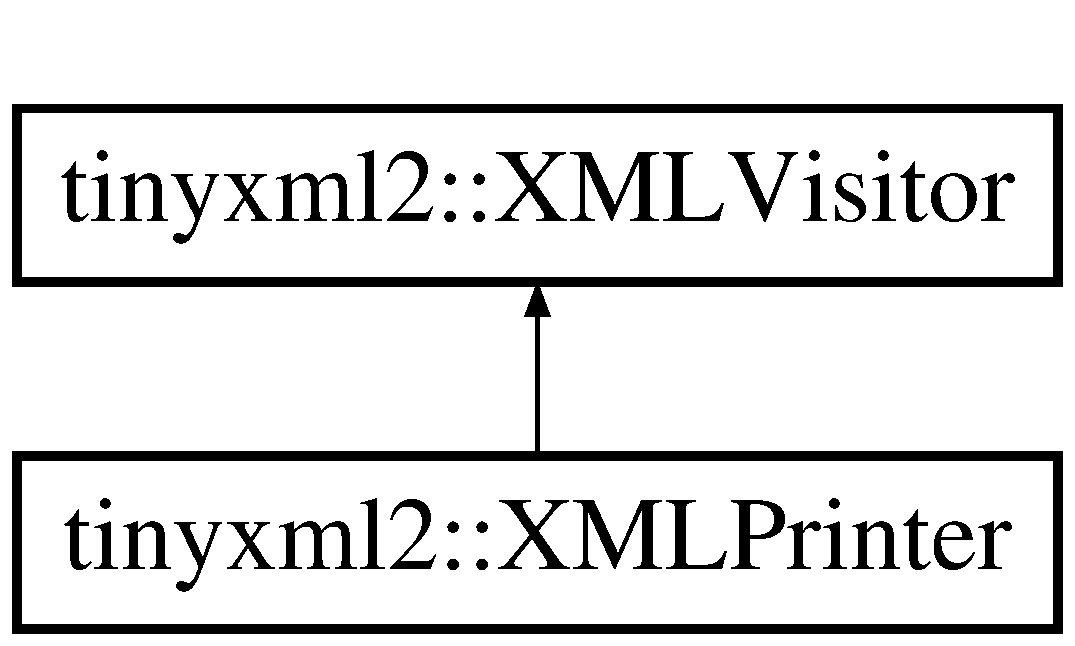
\includegraphics[height=2.000000cm]{classtinyxml2_1_1_x_m_l_printer}
\end{center}
\end{figure}
\subsection*{Public Member Functions}
\begin{DoxyCompactItemize}
\item 
\hyperlink{classtinyxml2_1_1_x_m_l_printer_aa6d3841c069085f5b8a27bc7103c04f7}{X\+M\+L\+Printer} (F\+I\+L\+E $\ast$file=0, bool compact=false, int depth=0)
\item 
virtual \hyperlink{classtinyxml2_1_1_x_m_l_printer_af4caefa48ea6436898fb1807de8d14c0}{$\sim$\+X\+M\+L\+Printer} ()
\item 
void \hyperlink{classtinyxml2_1_1_x_m_l_printer_a178c608ce8476043d5d6513819cde903}{Push\+Header} (bool write\+B\+O\+M, bool write\+Declaration)
\item 
void \hyperlink{classtinyxml2_1_1_x_m_l_printer_a20fb06c83bd13e5140d7dd13af06c010}{Open\+Element} (const char $\ast$name, bool compact\+Mode=false)
\item 
void \hyperlink{classtinyxml2_1_1_x_m_l_printer_a9a4e2c9348b42e147629d5a99f4af3f0}{Push\+Attribute} (const char $\ast$name, const char $\ast$value)
\begin{DoxyCompactList}\small\item\em If streaming, add an attribute to an open element. \end{DoxyCompactList}\item 
void \hyperlink{classtinyxml2_1_1_x_m_l_printer_a69120c82088597372d28d0a98f2ee7a1}{Push\+Attribute} (const char $\ast$name, int value)
\item 
void \hyperlink{classtinyxml2_1_1_x_m_l_printer_aa41039e51990aaf5342f3e0575a692c4}{Push\+Attribute} (const char $\ast$name, unsigned value)
\item 
void \hyperlink{classtinyxml2_1_1_x_m_l_printer_a51f7950d7b7a19f0d3a0d549a318d45f}{Push\+Attribute} (const char $\ast$name, bool value)
\item 
void \hyperlink{classtinyxml2_1_1_x_m_l_printer_a1714867af40e68ca404c3e84b6cac2a6}{Push\+Attribute} (const char $\ast$name, double value)
\item 
virtual void \hyperlink{classtinyxml2_1_1_x_m_l_printer_af1fb439e5d800999646f333fa2f0699a}{Close\+Element} (bool compact\+Mode=false)
\begin{DoxyCompactList}\small\item\em If streaming, close the Element. \end{DoxyCompactList}\item 
void \hyperlink{classtinyxml2_1_1_x_m_l_printer_a1cc16a9362df4332012cb13cff6441b3}{Push\+Text} (const char $\ast$text, bool cdata=false)
\begin{DoxyCompactList}\small\item\em Add a text node. \end{DoxyCompactList}\item 
void \hyperlink{classtinyxml2_1_1_x_m_l_printer_a3e0d4d78de25d4cf081009e1431cea7e}{Push\+Text} (int value)
\begin{DoxyCompactList}\small\item\em Add a text node from an integer. \end{DoxyCompactList}\item 
void \hyperlink{classtinyxml2_1_1_x_m_l_printer_a661fb50e7e0a4918d2d259cb0fae647e}{Push\+Text} (unsigned value)
\begin{DoxyCompactList}\small\item\em Add a text node from an unsigned. \end{DoxyCompactList}\item 
void \hyperlink{classtinyxml2_1_1_x_m_l_printer_a4390e5fa1ed05189a8686647345ab29f}{Push\+Text} (bool value)
\begin{DoxyCompactList}\small\item\em Add a text node from a bool. \end{DoxyCompactList}\item 
void \hyperlink{classtinyxml2_1_1_x_m_l_printer_a1dbb1390e829d0673af66b9cd1928bd7}{Push\+Text} (float value)
\begin{DoxyCompactList}\small\item\em Add a text node from a float. \end{DoxyCompactList}\item 
void \hyperlink{classtinyxml2_1_1_x_m_l_printer_aa715302dfc09473c77c853cbd5431965}{Push\+Text} (double value)
\begin{DoxyCompactList}\small\item\em Add a text node from a double. \end{DoxyCompactList}\item 
void \hyperlink{classtinyxml2_1_1_x_m_l_printer_afc8416814219591c2fd5656e0c233140}{Push\+Comment} (const char $\ast$comment)
\begin{DoxyCompactList}\small\item\em Add a comment. \end{DoxyCompactList}\item 
void \hyperlink{classtinyxml2_1_1_x_m_l_printer_a2fe3565e262594efc6c0276723c83fe7}{Push\+Declaration} (const char $\ast$value)
\item 
void \hyperlink{classtinyxml2_1_1_x_m_l_printer_ab1efc6d1548505e9984185f58f54b713}{Push\+Unknown} (const char $\ast$value)
\item 
virtual bool \hyperlink{classtinyxml2_1_1_x_m_l_printer_a9aa1de11a55a07db55a90fde37d7afad}{Visit\+Enter} (const \hyperlink{classtinyxml2_1_1_x_m_l_document}{X\+M\+L\+Document} \&)
\begin{DoxyCompactList}\small\item\em Visit a document. \end{DoxyCompactList}\item 
virtual bool \hyperlink{classtinyxml2_1_1_x_m_l_printer_a15fc1f2b922f540917dcf52808737b29}{Visit\+Exit} (const \hyperlink{classtinyxml2_1_1_x_m_l_document}{X\+M\+L\+Document} \&)
\begin{DoxyCompactList}\small\item\em Visit a document. \end{DoxyCompactList}\item 
virtual bool \hyperlink{classtinyxml2_1_1_x_m_l_printer_a169b2509d8eabb70811b2bb8cfd1f5d1}{Visit\+Enter} (const \hyperlink{classtinyxml2_1_1_x_m_l_element}{X\+M\+L\+Element} \&element, const \hyperlink{classtinyxml2_1_1_x_m_l_attribute}{X\+M\+L\+Attribute} $\ast$attribute)
\begin{DoxyCompactList}\small\item\em Visit an element. \end{DoxyCompactList}\item 
virtual bool \hyperlink{classtinyxml2_1_1_x_m_l_printer_a2edd48405971a88951c71c9df86a2f50}{Visit\+Exit} (const \hyperlink{classtinyxml2_1_1_x_m_l_element}{X\+M\+L\+Element} \&element)
\begin{DoxyCompactList}\small\item\em Visit an element. \end{DoxyCompactList}\item 
virtual bool \hyperlink{classtinyxml2_1_1_x_m_l_printer_adc0e42b4f6fcb90a95630c79575d030b}{Visit} (const \hyperlink{classtinyxml2_1_1_x_m_l_text}{X\+M\+L\+Text} \&text)
\begin{DoxyCompactList}\small\item\em Visit a text node. \end{DoxyCompactList}\item 
virtual bool \hyperlink{classtinyxml2_1_1_x_m_l_printer_aa294c5c01af0ebb9114902456e4cb53c}{Visit} (const \hyperlink{classtinyxml2_1_1_x_m_l_comment}{X\+M\+L\+Comment} \&comment)
\begin{DoxyCompactList}\small\item\em Visit a comment node. \end{DoxyCompactList}\item 
virtual bool \hyperlink{classtinyxml2_1_1_x_m_l_printer_acfc625b2549304b9c7eb85ebd5c5eb39}{Visit} (const \hyperlink{classtinyxml2_1_1_x_m_l_declaration}{X\+M\+L\+Declaration} \&declaration)
\begin{DoxyCompactList}\small\item\em Visit a declaration. \end{DoxyCompactList}\item 
virtual bool \hyperlink{classtinyxml2_1_1_x_m_l_printer_ab8af5455bbf9e4be2663e6642fcd7e32}{Visit} (const \hyperlink{classtinyxml2_1_1_x_m_l_unknown}{X\+M\+L\+Unknown} \&unknown)
\begin{DoxyCompactList}\small\item\em Visit an unknown node. \end{DoxyCompactList}\item 
const char $\ast$ \hyperlink{classtinyxml2_1_1_x_m_l_printer_a4a1b788e11b540921ec50687cd2b24a9}{C\+Str} () const 
\item 
int \hyperlink{classtinyxml2_1_1_x_m_l_printer_a02c3c5f8c6c007dcbaf10595d9e22bf0}{C\+Str\+Size} () const 
\item 
void \hyperlink{classtinyxml2_1_1_x_m_l_printer_a216157765b7267bf389975b1cbf9a909}{Clear\+Buffer} ()
\end{DoxyCompactItemize}
\subsection*{Protected Member Functions}
\begin{DoxyCompactItemize}
\item 
virtual bool \hyperlink{classtinyxml2_1_1_x_m_l_printer_a38e1ed5a779bdf63eda9e808f7a6de66}{Compact\+Mode} (const \hyperlink{classtinyxml2_1_1_x_m_l_element}{X\+M\+L\+Element} \&)
\item 
virtual void \hyperlink{classtinyxml2_1_1_x_m_l_printer_a1c4b2ccbe4fdb316d54f5a93f3559260}{Print\+Space} (int depth)
\item 
void \hyperlink{classtinyxml2_1_1_x_m_l_printer_ab30210a7f32e45634e7a45137bf6fdf6}{Print} (const char $\ast$format,...)
\item 
void \hyperlink{classtinyxml2_1_1_x_m_l_printer_ac6e2c72c5d796f5b4de6ce81ca95e3fa}{Seal\+Element\+If\+Just\+Opened} ()
\end{DoxyCompactItemize}
\subsection*{Protected Attributes}
\begin{DoxyCompactItemize}
\item 
bool \hyperlink{classtinyxml2_1_1_x_m_l_printer_ac07169d58b465214a2b1fa306e617c26}{\+\_\+element\+Just\+Opened}
\item 
\hyperlink{classtinyxml2_1_1_dyn_array}{Dyn\+Array}$<$ const char $\ast$, 10 $>$ \hyperlink{classtinyxml2_1_1_x_m_l_printer_a99d59e67e084714541bee3ae43884bef}{\+\_\+stack}
\end{DoxyCompactItemize}


\subsection{Detailed Description}
Printing functionality. The \hyperlink{classtinyxml2_1_1_x_m_l_printer}{X\+M\+L\+Printer} gives you more options than the \hyperlink{classtinyxml2_1_1_x_m_l_document_a686ea28672c0e0c60383ec28148c1ac0}{X\+M\+L\+Document\+::\+Print()} method.

It can\+:
\begin{DoxyEnumerate}
\item Print to memory.
\item Print to a file you provide.
\item Print X\+M\+L without a \hyperlink{classtinyxml2_1_1_x_m_l_document}{X\+M\+L\+Document}.
\end{DoxyEnumerate}

Print to Memory

\begin{DoxyVerb}XMLPrinter printer;
doc.Print( &printer );
SomeFunction( printer.CStr() );
\end{DoxyVerb}


Print to a File

You provide the file pointer. \begin{DoxyVerb}XMLPrinter printer( fp );
doc.Print( &printer );
\end{DoxyVerb}


Print without a \hyperlink{classtinyxml2_1_1_x_m_l_document}{X\+M\+L\+Document}

When loading, an X\+M\+L parser is very useful. However, sometimes when saving, it just gets in the way. The code is often set up for streaming, and constructing the D\+O\+M is just overhead.

The Printer supports the streaming case. The following code prints out a trivially simple X\+M\+L file without ever creating an X\+M\+L document.

\begin{DoxyVerb}XMLPrinter printer( fp );
printer.OpenElement( "foo" );
printer.PushAttribute( "foo", "bar" );
printer.CloseElement();
\end{DoxyVerb}
 

\subsection{Constructor \& Destructor Documentation}
\hypertarget{classtinyxml2_1_1_x_m_l_printer_aa6d3841c069085f5b8a27bc7103c04f7}{}\index{tinyxml2\+::\+X\+M\+L\+Printer@{tinyxml2\+::\+X\+M\+L\+Printer}!X\+M\+L\+Printer@{X\+M\+L\+Printer}}
\index{X\+M\+L\+Printer@{X\+M\+L\+Printer}!tinyxml2\+::\+X\+M\+L\+Printer@{tinyxml2\+::\+X\+M\+L\+Printer}}
\subsubsection[{X\+M\+L\+Printer}]{\setlength{\rightskip}{0pt plus 5cm}tinyxml2\+::\+X\+M\+L\+Printer\+::\+X\+M\+L\+Printer (
\begin{DoxyParamCaption}
\item[{F\+I\+L\+E $\ast$}]{file = {\ttfamily 0}, }
\item[{bool}]{compact = {\ttfamily false}, }
\item[{int}]{depth = {\ttfamily 0}}
\end{DoxyParamCaption}
)}\label{classtinyxml2_1_1_x_m_l_printer_aa6d3841c069085f5b8a27bc7103c04f7}
Construct the printer. If the F\+I\+L\+E$\ast$ is specified, this will print to the F\+I\+L\+E. Else it will print to memory, and the result is available in \hyperlink{classtinyxml2_1_1_x_m_l_printer_a4a1b788e11b540921ec50687cd2b24a9}{C\+Str()}. If \textquotesingle{}compact\textquotesingle{} is set to true, then output is created with only required whitespace and newlines. \hypertarget{classtinyxml2_1_1_x_m_l_printer_af4caefa48ea6436898fb1807de8d14c0}{}\index{tinyxml2\+::\+X\+M\+L\+Printer@{tinyxml2\+::\+X\+M\+L\+Printer}!````~X\+M\+L\+Printer@{$\sim$\+X\+M\+L\+Printer}}
\index{````~X\+M\+L\+Printer@{$\sim$\+X\+M\+L\+Printer}!tinyxml2\+::\+X\+M\+L\+Printer@{tinyxml2\+::\+X\+M\+L\+Printer}}
\subsubsection[{$\sim$\+X\+M\+L\+Printer}]{\setlength{\rightskip}{0pt plus 5cm}virtual tinyxml2\+::\+X\+M\+L\+Printer\+::$\sim$\+X\+M\+L\+Printer (
\begin{DoxyParamCaption}
{}
\end{DoxyParamCaption}
)\hspace{0.3cm}{\ttfamily [inline]}, {\ttfamily [virtual]}}\label{classtinyxml2_1_1_x_m_l_printer_af4caefa48ea6436898fb1807de8d14c0}


\subsection{Member Function Documentation}
\hypertarget{classtinyxml2_1_1_x_m_l_printer_a216157765b7267bf389975b1cbf9a909}{}\index{tinyxml2\+::\+X\+M\+L\+Printer@{tinyxml2\+::\+X\+M\+L\+Printer}!Clear\+Buffer@{Clear\+Buffer}}
\index{Clear\+Buffer@{Clear\+Buffer}!tinyxml2\+::\+X\+M\+L\+Printer@{tinyxml2\+::\+X\+M\+L\+Printer}}
\subsubsection[{Clear\+Buffer}]{\setlength{\rightskip}{0pt plus 5cm}void tinyxml2\+::\+X\+M\+L\+Printer\+::\+Clear\+Buffer (
\begin{DoxyParamCaption}
{}
\end{DoxyParamCaption}
)\hspace{0.3cm}{\ttfamily [inline]}}\label{classtinyxml2_1_1_x_m_l_printer_a216157765b7267bf389975b1cbf9a909}
If in print to memory mode, reset the buffer to the beginning. \hypertarget{classtinyxml2_1_1_x_m_l_printer_af1fb439e5d800999646f333fa2f0699a}{}\index{tinyxml2\+::\+X\+M\+L\+Printer@{tinyxml2\+::\+X\+M\+L\+Printer}!Close\+Element@{Close\+Element}}
\index{Close\+Element@{Close\+Element}!tinyxml2\+::\+X\+M\+L\+Printer@{tinyxml2\+::\+X\+M\+L\+Printer}}
\subsubsection[{Close\+Element}]{\setlength{\rightskip}{0pt plus 5cm}void tinyxml2\+::\+X\+M\+L\+Printer\+::\+Close\+Element (
\begin{DoxyParamCaption}
\item[{bool}]{compact\+Mode = {\ttfamily false}}
\end{DoxyParamCaption}
)\hspace{0.3cm}{\ttfamily [virtual]}}\label{classtinyxml2_1_1_x_m_l_printer_af1fb439e5d800999646f333fa2f0699a}


If streaming, close the Element. 

\hypertarget{classtinyxml2_1_1_x_m_l_printer_a38e1ed5a779bdf63eda9e808f7a6de66}{}\index{tinyxml2\+::\+X\+M\+L\+Printer@{tinyxml2\+::\+X\+M\+L\+Printer}!Compact\+Mode@{Compact\+Mode}}
\index{Compact\+Mode@{Compact\+Mode}!tinyxml2\+::\+X\+M\+L\+Printer@{tinyxml2\+::\+X\+M\+L\+Printer}}
\subsubsection[{Compact\+Mode}]{\setlength{\rightskip}{0pt plus 5cm}virtual bool tinyxml2\+::\+X\+M\+L\+Printer\+::\+Compact\+Mode (
\begin{DoxyParamCaption}
\item[{const {\bf X\+M\+L\+Element} \&}]{}
\end{DoxyParamCaption}
)\hspace{0.3cm}{\ttfamily [inline]}, {\ttfamily [protected]}, {\ttfamily [virtual]}}\label{classtinyxml2_1_1_x_m_l_printer_a38e1ed5a779bdf63eda9e808f7a6de66}
\hypertarget{classtinyxml2_1_1_x_m_l_printer_a4a1b788e11b540921ec50687cd2b24a9}{}\index{tinyxml2\+::\+X\+M\+L\+Printer@{tinyxml2\+::\+X\+M\+L\+Printer}!C\+Str@{C\+Str}}
\index{C\+Str@{C\+Str}!tinyxml2\+::\+X\+M\+L\+Printer@{tinyxml2\+::\+X\+M\+L\+Printer}}
\subsubsection[{C\+Str}]{\setlength{\rightskip}{0pt plus 5cm}const char$\ast$ tinyxml2\+::\+X\+M\+L\+Printer\+::\+C\+Str (
\begin{DoxyParamCaption}
{}
\end{DoxyParamCaption}
) const\hspace{0.3cm}{\ttfamily [inline]}}\label{classtinyxml2_1_1_x_m_l_printer_a4a1b788e11b540921ec50687cd2b24a9}
If in print to memory mode, return a pointer to the X\+M\+L file in memory. \hypertarget{classtinyxml2_1_1_x_m_l_printer_a02c3c5f8c6c007dcbaf10595d9e22bf0}{}\index{tinyxml2\+::\+X\+M\+L\+Printer@{tinyxml2\+::\+X\+M\+L\+Printer}!C\+Str\+Size@{C\+Str\+Size}}
\index{C\+Str\+Size@{C\+Str\+Size}!tinyxml2\+::\+X\+M\+L\+Printer@{tinyxml2\+::\+X\+M\+L\+Printer}}
\subsubsection[{C\+Str\+Size}]{\setlength{\rightskip}{0pt plus 5cm}int tinyxml2\+::\+X\+M\+L\+Printer\+::\+C\+Str\+Size (
\begin{DoxyParamCaption}
{}
\end{DoxyParamCaption}
) const\hspace{0.3cm}{\ttfamily [inline]}}\label{classtinyxml2_1_1_x_m_l_printer_a02c3c5f8c6c007dcbaf10595d9e22bf0}
If in print to memory mode, return the size of the X\+M\+L file in memory. (Note the size returned includes the terminating null.) \hypertarget{classtinyxml2_1_1_x_m_l_printer_a20fb06c83bd13e5140d7dd13af06c010}{}\index{tinyxml2\+::\+X\+M\+L\+Printer@{tinyxml2\+::\+X\+M\+L\+Printer}!Open\+Element@{Open\+Element}}
\index{Open\+Element@{Open\+Element}!tinyxml2\+::\+X\+M\+L\+Printer@{tinyxml2\+::\+X\+M\+L\+Printer}}
\subsubsection[{Open\+Element}]{\setlength{\rightskip}{0pt plus 5cm}void tinyxml2\+::\+X\+M\+L\+Printer\+::\+Open\+Element (
\begin{DoxyParamCaption}
\item[{const char $\ast$}]{name, }
\item[{bool}]{compact\+Mode = {\ttfamily false}}
\end{DoxyParamCaption}
)}\label{classtinyxml2_1_1_x_m_l_printer_a20fb06c83bd13e5140d7dd13af06c010}
If streaming, start writing an element. The element must be closed with \hyperlink{classtinyxml2_1_1_x_m_l_printer_af1fb439e5d800999646f333fa2f0699a}{Close\+Element()} \hypertarget{classtinyxml2_1_1_x_m_l_printer_ab30210a7f32e45634e7a45137bf6fdf6}{}\index{tinyxml2\+::\+X\+M\+L\+Printer@{tinyxml2\+::\+X\+M\+L\+Printer}!Print@{Print}}
\index{Print@{Print}!tinyxml2\+::\+X\+M\+L\+Printer@{tinyxml2\+::\+X\+M\+L\+Printer}}
\subsubsection[{Print}]{\setlength{\rightskip}{0pt plus 5cm}void tinyxml2\+::\+X\+M\+L\+Printer\+::\+Print (
\begin{DoxyParamCaption}
\item[{const char $\ast$}]{format, }
\item[{}]{...}
\end{DoxyParamCaption}
)\hspace{0.3cm}{\ttfamily [protected]}}\label{classtinyxml2_1_1_x_m_l_printer_ab30210a7f32e45634e7a45137bf6fdf6}
\hypertarget{classtinyxml2_1_1_x_m_l_printer_a1c4b2ccbe4fdb316d54f5a93f3559260}{}\index{tinyxml2\+::\+X\+M\+L\+Printer@{tinyxml2\+::\+X\+M\+L\+Printer}!Print\+Space@{Print\+Space}}
\index{Print\+Space@{Print\+Space}!tinyxml2\+::\+X\+M\+L\+Printer@{tinyxml2\+::\+X\+M\+L\+Printer}}
\subsubsection[{Print\+Space}]{\setlength{\rightskip}{0pt plus 5cm}void tinyxml2\+::\+X\+M\+L\+Printer\+::\+Print\+Space (
\begin{DoxyParamCaption}
\item[{int}]{depth}
\end{DoxyParamCaption}
)\hspace{0.3cm}{\ttfamily [protected]}, {\ttfamily [virtual]}}\label{classtinyxml2_1_1_x_m_l_printer_a1c4b2ccbe4fdb316d54f5a93f3559260}
Prints out the space before an element. You may override to change the space and tabs used. A \hyperlink{classtinyxml2_1_1_x_m_l_printer_a1c4b2ccbe4fdb316d54f5a93f3559260}{Print\+Space()} override should call \hyperlink{classtinyxml2_1_1_x_m_l_printer_ab30210a7f32e45634e7a45137bf6fdf6}{Print()}. \hypertarget{classtinyxml2_1_1_x_m_l_printer_a9a4e2c9348b42e147629d5a99f4af3f0}{}\index{tinyxml2\+::\+X\+M\+L\+Printer@{tinyxml2\+::\+X\+M\+L\+Printer}!Push\+Attribute@{Push\+Attribute}}
\index{Push\+Attribute@{Push\+Attribute}!tinyxml2\+::\+X\+M\+L\+Printer@{tinyxml2\+::\+X\+M\+L\+Printer}}
\subsubsection[{Push\+Attribute}]{\setlength{\rightskip}{0pt plus 5cm}void tinyxml2\+::\+X\+M\+L\+Printer\+::\+Push\+Attribute (
\begin{DoxyParamCaption}
\item[{const char $\ast$}]{name, }
\item[{const char $\ast$}]{value}
\end{DoxyParamCaption}
)}\label{classtinyxml2_1_1_x_m_l_printer_a9a4e2c9348b42e147629d5a99f4af3f0}


If streaming, add an attribute to an open element. 

\hypertarget{classtinyxml2_1_1_x_m_l_printer_a69120c82088597372d28d0a98f2ee7a1}{}\index{tinyxml2\+::\+X\+M\+L\+Printer@{tinyxml2\+::\+X\+M\+L\+Printer}!Push\+Attribute@{Push\+Attribute}}
\index{Push\+Attribute@{Push\+Attribute}!tinyxml2\+::\+X\+M\+L\+Printer@{tinyxml2\+::\+X\+M\+L\+Printer}}
\subsubsection[{Push\+Attribute}]{\setlength{\rightskip}{0pt plus 5cm}void tinyxml2\+::\+X\+M\+L\+Printer\+::\+Push\+Attribute (
\begin{DoxyParamCaption}
\item[{const char $\ast$}]{name, }
\item[{int}]{value}
\end{DoxyParamCaption}
)}\label{classtinyxml2_1_1_x_m_l_printer_a69120c82088597372d28d0a98f2ee7a1}
\hypertarget{classtinyxml2_1_1_x_m_l_printer_aa41039e51990aaf5342f3e0575a692c4}{}\index{tinyxml2\+::\+X\+M\+L\+Printer@{tinyxml2\+::\+X\+M\+L\+Printer}!Push\+Attribute@{Push\+Attribute}}
\index{Push\+Attribute@{Push\+Attribute}!tinyxml2\+::\+X\+M\+L\+Printer@{tinyxml2\+::\+X\+M\+L\+Printer}}
\subsubsection[{Push\+Attribute}]{\setlength{\rightskip}{0pt plus 5cm}void tinyxml2\+::\+X\+M\+L\+Printer\+::\+Push\+Attribute (
\begin{DoxyParamCaption}
\item[{const char $\ast$}]{name, }
\item[{unsigned}]{value}
\end{DoxyParamCaption}
)}\label{classtinyxml2_1_1_x_m_l_printer_aa41039e51990aaf5342f3e0575a692c4}
\hypertarget{classtinyxml2_1_1_x_m_l_printer_a51f7950d7b7a19f0d3a0d549a318d45f}{}\index{tinyxml2\+::\+X\+M\+L\+Printer@{tinyxml2\+::\+X\+M\+L\+Printer}!Push\+Attribute@{Push\+Attribute}}
\index{Push\+Attribute@{Push\+Attribute}!tinyxml2\+::\+X\+M\+L\+Printer@{tinyxml2\+::\+X\+M\+L\+Printer}}
\subsubsection[{Push\+Attribute}]{\setlength{\rightskip}{0pt plus 5cm}void tinyxml2\+::\+X\+M\+L\+Printer\+::\+Push\+Attribute (
\begin{DoxyParamCaption}
\item[{const char $\ast$}]{name, }
\item[{bool}]{value}
\end{DoxyParamCaption}
)}\label{classtinyxml2_1_1_x_m_l_printer_a51f7950d7b7a19f0d3a0d549a318d45f}
\hypertarget{classtinyxml2_1_1_x_m_l_printer_a1714867af40e68ca404c3e84b6cac2a6}{}\index{tinyxml2\+::\+X\+M\+L\+Printer@{tinyxml2\+::\+X\+M\+L\+Printer}!Push\+Attribute@{Push\+Attribute}}
\index{Push\+Attribute@{Push\+Attribute}!tinyxml2\+::\+X\+M\+L\+Printer@{tinyxml2\+::\+X\+M\+L\+Printer}}
\subsubsection[{Push\+Attribute}]{\setlength{\rightskip}{0pt plus 5cm}void tinyxml2\+::\+X\+M\+L\+Printer\+::\+Push\+Attribute (
\begin{DoxyParamCaption}
\item[{const char $\ast$}]{name, }
\item[{double}]{value}
\end{DoxyParamCaption}
)}\label{classtinyxml2_1_1_x_m_l_printer_a1714867af40e68ca404c3e84b6cac2a6}
\hypertarget{classtinyxml2_1_1_x_m_l_printer_afc8416814219591c2fd5656e0c233140}{}\index{tinyxml2\+::\+X\+M\+L\+Printer@{tinyxml2\+::\+X\+M\+L\+Printer}!Push\+Comment@{Push\+Comment}}
\index{Push\+Comment@{Push\+Comment}!tinyxml2\+::\+X\+M\+L\+Printer@{tinyxml2\+::\+X\+M\+L\+Printer}}
\subsubsection[{Push\+Comment}]{\setlength{\rightskip}{0pt plus 5cm}void tinyxml2\+::\+X\+M\+L\+Printer\+::\+Push\+Comment (
\begin{DoxyParamCaption}
\item[{const char $\ast$}]{comment}
\end{DoxyParamCaption}
)}\label{classtinyxml2_1_1_x_m_l_printer_afc8416814219591c2fd5656e0c233140}


Add a comment. 

\hypertarget{classtinyxml2_1_1_x_m_l_printer_a2fe3565e262594efc6c0276723c83fe7}{}\index{tinyxml2\+::\+X\+M\+L\+Printer@{tinyxml2\+::\+X\+M\+L\+Printer}!Push\+Declaration@{Push\+Declaration}}
\index{Push\+Declaration@{Push\+Declaration}!tinyxml2\+::\+X\+M\+L\+Printer@{tinyxml2\+::\+X\+M\+L\+Printer}}
\subsubsection[{Push\+Declaration}]{\setlength{\rightskip}{0pt plus 5cm}void tinyxml2\+::\+X\+M\+L\+Printer\+::\+Push\+Declaration (
\begin{DoxyParamCaption}
\item[{const char $\ast$}]{value}
\end{DoxyParamCaption}
)}\label{classtinyxml2_1_1_x_m_l_printer_a2fe3565e262594efc6c0276723c83fe7}
\hypertarget{classtinyxml2_1_1_x_m_l_printer_a178c608ce8476043d5d6513819cde903}{}\index{tinyxml2\+::\+X\+M\+L\+Printer@{tinyxml2\+::\+X\+M\+L\+Printer}!Push\+Header@{Push\+Header}}
\index{Push\+Header@{Push\+Header}!tinyxml2\+::\+X\+M\+L\+Printer@{tinyxml2\+::\+X\+M\+L\+Printer}}
\subsubsection[{Push\+Header}]{\setlength{\rightskip}{0pt plus 5cm}void tinyxml2\+::\+X\+M\+L\+Printer\+::\+Push\+Header (
\begin{DoxyParamCaption}
\item[{bool}]{write\+B\+O\+M, }
\item[{bool}]{write\+Declaration}
\end{DoxyParamCaption}
)}\label{classtinyxml2_1_1_x_m_l_printer_a178c608ce8476043d5d6513819cde903}
If streaming, write the B\+O\+M and declaration. \hypertarget{classtinyxml2_1_1_x_m_l_printer_a1cc16a9362df4332012cb13cff6441b3}{}\index{tinyxml2\+::\+X\+M\+L\+Printer@{tinyxml2\+::\+X\+M\+L\+Printer}!Push\+Text@{Push\+Text}}
\index{Push\+Text@{Push\+Text}!tinyxml2\+::\+X\+M\+L\+Printer@{tinyxml2\+::\+X\+M\+L\+Printer}}
\subsubsection[{Push\+Text}]{\setlength{\rightskip}{0pt plus 5cm}void tinyxml2\+::\+X\+M\+L\+Printer\+::\+Push\+Text (
\begin{DoxyParamCaption}
\item[{const char $\ast$}]{text, }
\item[{bool}]{cdata = {\ttfamily false}}
\end{DoxyParamCaption}
)}\label{classtinyxml2_1_1_x_m_l_printer_a1cc16a9362df4332012cb13cff6441b3}


Add a text node. 

\hypertarget{classtinyxml2_1_1_x_m_l_printer_a3e0d4d78de25d4cf081009e1431cea7e}{}\index{tinyxml2\+::\+X\+M\+L\+Printer@{tinyxml2\+::\+X\+M\+L\+Printer}!Push\+Text@{Push\+Text}}
\index{Push\+Text@{Push\+Text}!tinyxml2\+::\+X\+M\+L\+Printer@{tinyxml2\+::\+X\+M\+L\+Printer}}
\subsubsection[{Push\+Text}]{\setlength{\rightskip}{0pt plus 5cm}void tinyxml2\+::\+X\+M\+L\+Printer\+::\+Push\+Text (
\begin{DoxyParamCaption}
\item[{int}]{value}
\end{DoxyParamCaption}
)}\label{classtinyxml2_1_1_x_m_l_printer_a3e0d4d78de25d4cf081009e1431cea7e}


Add a text node from an integer. 

\hypertarget{classtinyxml2_1_1_x_m_l_printer_a661fb50e7e0a4918d2d259cb0fae647e}{}\index{tinyxml2\+::\+X\+M\+L\+Printer@{tinyxml2\+::\+X\+M\+L\+Printer}!Push\+Text@{Push\+Text}}
\index{Push\+Text@{Push\+Text}!tinyxml2\+::\+X\+M\+L\+Printer@{tinyxml2\+::\+X\+M\+L\+Printer}}
\subsubsection[{Push\+Text}]{\setlength{\rightskip}{0pt plus 5cm}void tinyxml2\+::\+X\+M\+L\+Printer\+::\+Push\+Text (
\begin{DoxyParamCaption}
\item[{unsigned}]{value}
\end{DoxyParamCaption}
)}\label{classtinyxml2_1_1_x_m_l_printer_a661fb50e7e0a4918d2d259cb0fae647e}


Add a text node from an unsigned. 

\hypertarget{classtinyxml2_1_1_x_m_l_printer_a4390e5fa1ed05189a8686647345ab29f}{}\index{tinyxml2\+::\+X\+M\+L\+Printer@{tinyxml2\+::\+X\+M\+L\+Printer}!Push\+Text@{Push\+Text}}
\index{Push\+Text@{Push\+Text}!tinyxml2\+::\+X\+M\+L\+Printer@{tinyxml2\+::\+X\+M\+L\+Printer}}
\subsubsection[{Push\+Text}]{\setlength{\rightskip}{0pt plus 5cm}void tinyxml2\+::\+X\+M\+L\+Printer\+::\+Push\+Text (
\begin{DoxyParamCaption}
\item[{bool}]{value}
\end{DoxyParamCaption}
)}\label{classtinyxml2_1_1_x_m_l_printer_a4390e5fa1ed05189a8686647345ab29f}


Add a text node from a bool. 

\hypertarget{classtinyxml2_1_1_x_m_l_printer_a1dbb1390e829d0673af66b9cd1928bd7}{}\index{tinyxml2\+::\+X\+M\+L\+Printer@{tinyxml2\+::\+X\+M\+L\+Printer}!Push\+Text@{Push\+Text}}
\index{Push\+Text@{Push\+Text}!tinyxml2\+::\+X\+M\+L\+Printer@{tinyxml2\+::\+X\+M\+L\+Printer}}
\subsubsection[{Push\+Text}]{\setlength{\rightskip}{0pt plus 5cm}void tinyxml2\+::\+X\+M\+L\+Printer\+::\+Push\+Text (
\begin{DoxyParamCaption}
\item[{float}]{value}
\end{DoxyParamCaption}
)}\label{classtinyxml2_1_1_x_m_l_printer_a1dbb1390e829d0673af66b9cd1928bd7}


Add a text node from a float. 

\hypertarget{classtinyxml2_1_1_x_m_l_printer_aa715302dfc09473c77c853cbd5431965}{}\index{tinyxml2\+::\+X\+M\+L\+Printer@{tinyxml2\+::\+X\+M\+L\+Printer}!Push\+Text@{Push\+Text}}
\index{Push\+Text@{Push\+Text}!tinyxml2\+::\+X\+M\+L\+Printer@{tinyxml2\+::\+X\+M\+L\+Printer}}
\subsubsection[{Push\+Text}]{\setlength{\rightskip}{0pt plus 5cm}void tinyxml2\+::\+X\+M\+L\+Printer\+::\+Push\+Text (
\begin{DoxyParamCaption}
\item[{double}]{value}
\end{DoxyParamCaption}
)}\label{classtinyxml2_1_1_x_m_l_printer_aa715302dfc09473c77c853cbd5431965}


Add a text node from a double. 

\hypertarget{classtinyxml2_1_1_x_m_l_printer_ab1efc6d1548505e9984185f58f54b713}{}\index{tinyxml2\+::\+X\+M\+L\+Printer@{tinyxml2\+::\+X\+M\+L\+Printer}!Push\+Unknown@{Push\+Unknown}}
\index{Push\+Unknown@{Push\+Unknown}!tinyxml2\+::\+X\+M\+L\+Printer@{tinyxml2\+::\+X\+M\+L\+Printer}}
\subsubsection[{Push\+Unknown}]{\setlength{\rightskip}{0pt plus 5cm}void tinyxml2\+::\+X\+M\+L\+Printer\+::\+Push\+Unknown (
\begin{DoxyParamCaption}
\item[{const char $\ast$}]{value}
\end{DoxyParamCaption}
)}\label{classtinyxml2_1_1_x_m_l_printer_ab1efc6d1548505e9984185f58f54b713}
\hypertarget{classtinyxml2_1_1_x_m_l_printer_ac6e2c72c5d796f5b4de6ce81ca95e3fa}{}\index{tinyxml2\+::\+X\+M\+L\+Printer@{tinyxml2\+::\+X\+M\+L\+Printer}!Seal\+Element\+If\+Just\+Opened@{Seal\+Element\+If\+Just\+Opened}}
\index{Seal\+Element\+If\+Just\+Opened@{Seal\+Element\+If\+Just\+Opened}!tinyxml2\+::\+X\+M\+L\+Printer@{tinyxml2\+::\+X\+M\+L\+Printer}}
\subsubsection[{Seal\+Element\+If\+Just\+Opened}]{\setlength{\rightskip}{0pt plus 5cm}void tinyxml2\+::\+X\+M\+L\+Printer\+::\+Seal\+Element\+If\+Just\+Opened (
\begin{DoxyParamCaption}
{}
\end{DoxyParamCaption}
)\hspace{0.3cm}{\ttfamily [protected]}}\label{classtinyxml2_1_1_x_m_l_printer_ac6e2c72c5d796f5b4de6ce81ca95e3fa}
\hypertarget{classtinyxml2_1_1_x_m_l_printer_adc0e42b4f6fcb90a95630c79575d030b}{}\index{tinyxml2\+::\+X\+M\+L\+Printer@{tinyxml2\+::\+X\+M\+L\+Printer}!Visit@{Visit}}
\index{Visit@{Visit}!tinyxml2\+::\+X\+M\+L\+Printer@{tinyxml2\+::\+X\+M\+L\+Printer}}
\subsubsection[{Visit}]{\setlength{\rightskip}{0pt plus 5cm}bool tinyxml2\+::\+X\+M\+L\+Printer\+::\+Visit (
\begin{DoxyParamCaption}
\item[{const {\bf X\+M\+L\+Text} \&}]{}
\end{DoxyParamCaption}
)\hspace{0.3cm}{\ttfamily [virtual]}}\label{classtinyxml2_1_1_x_m_l_printer_adc0e42b4f6fcb90a95630c79575d030b}


Visit a text node. 



Reimplemented from \hyperlink{classtinyxml2_1_1_x_m_l_visitor_af30233565856480ea48b6fa0d6dec65b}{tinyxml2\+::\+X\+M\+L\+Visitor}.

\hypertarget{classtinyxml2_1_1_x_m_l_printer_aa294c5c01af0ebb9114902456e4cb53c}{}\index{tinyxml2\+::\+X\+M\+L\+Printer@{tinyxml2\+::\+X\+M\+L\+Printer}!Visit@{Visit}}
\index{Visit@{Visit}!tinyxml2\+::\+X\+M\+L\+Printer@{tinyxml2\+::\+X\+M\+L\+Printer}}
\subsubsection[{Visit}]{\setlength{\rightskip}{0pt plus 5cm}bool tinyxml2\+::\+X\+M\+L\+Printer\+::\+Visit (
\begin{DoxyParamCaption}
\item[{const {\bf X\+M\+L\+Comment} \&}]{}
\end{DoxyParamCaption}
)\hspace{0.3cm}{\ttfamily [virtual]}}\label{classtinyxml2_1_1_x_m_l_printer_aa294c5c01af0ebb9114902456e4cb53c}


Visit a comment node. 



Reimplemented from \hyperlink{classtinyxml2_1_1_x_m_l_visitor_acc8147fb5a85f6c65721654e427752d7}{tinyxml2\+::\+X\+M\+L\+Visitor}.

\hypertarget{classtinyxml2_1_1_x_m_l_printer_acfc625b2549304b9c7eb85ebd5c5eb39}{}\index{tinyxml2\+::\+X\+M\+L\+Printer@{tinyxml2\+::\+X\+M\+L\+Printer}!Visit@{Visit}}
\index{Visit@{Visit}!tinyxml2\+::\+X\+M\+L\+Printer@{tinyxml2\+::\+X\+M\+L\+Printer}}
\subsubsection[{Visit}]{\setlength{\rightskip}{0pt plus 5cm}bool tinyxml2\+::\+X\+M\+L\+Printer\+::\+Visit (
\begin{DoxyParamCaption}
\item[{const {\bf X\+M\+L\+Declaration} \&}]{}
\end{DoxyParamCaption}
)\hspace{0.3cm}{\ttfamily [virtual]}}\label{classtinyxml2_1_1_x_m_l_printer_acfc625b2549304b9c7eb85ebd5c5eb39}


Visit a declaration. 



Reimplemented from \hyperlink{classtinyxml2_1_1_x_m_l_visitor_adc75bd459fc7ba8223b50f0616767f9a}{tinyxml2\+::\+X\+M\+L\+Visitor}.

\hypertarget{classtinyxml2_1_1_x_m_l_printer_ab8af5455bbf9e4be2663e6642fcd7e32}{}\index{tinyxml2\+::\+X\+M\+L\+Printer@{tinyxml2\+::\+X\+M\+L\+Printer}!Visit@{Visit}}
\index{Visit@{Visit}!tinyxml2\+::\+X\+M\+L\+Printer@{tinyxml2\+::\+X\+M\+L\+Printer}}
\subsubsection[{Visit}]{\setlength{\rightskip}{0pt plus 5cm}bool tinyxml2\+::\+X\+M\+L\+Printer\+::\+Visit (
\begin{DoxyParamCaption}
\item[{const {\bf X\+M\+L\+Unknown} \&}]{}
\end{DoxyParamCaption}
)\hspace{0.3cm}{\ttfamily [virtual]}}\label{classtinyxml2_1_1_x_m_l_printer_ab8af5455bbf9e4be2663e6642fcd7e32}


Visit an unknown node. 



Reimplemented from \hyperlink{classtinyxml2_1_1_x_m_l_visitor_a14e4748387c34bf53d24e8119bb1f292}{tinyxml2\+::\+X\+M\+L\+Visitor}.

\hypertarget{classtinyxml2_1_1_x_m_l_printer_a9aa1de11a55a07db55a90fde37d7afad}{}\index{tinyxml2\+::\+X\+M\+L\+Printer@{tinyxml2\+::\+X\+M\+L\+Printer}!Visit\+Enter@{Visit\+Enter}}
\index{Visit\+Enter@{Visit\+Enter}!tinyxml2\+::\+X\+M\+L\+Printer@{tinyxml2\+::\+X\+M\+L\+Printer}}
\subsubsection[{Visit\+Enter}]{\setlength{\rightskip}{0pt plus 5cm}bool tinyxml2\+::\+X\+M\+L\+Printer\+::\+Visit\+Enter (
\begin{DoxyParamCaption}
\item[{const {\bf X\+M\+L\+Document} \&}]{}
\end{DoxyParamCaption}
)\hspace{0.3cm}{\ttfamily [virtual]}}\label{classtinyxml2_1_1_x_m_l_printer_a9aa1de11a55a07db55a90fde37d7afad}


Visit a document. 



Reimplemented from \hyperlink{classtinyxml2_1_1_x_m_l_visitor_acb3c22fc5f60eb9db98f533f2761f67d}{tinyxml2\+::\+X\+M\+L\+Visitor}.

\hypertarget{classtinyxml2_1_1_x_m_l_printer_a169b2509d8eabb70811b2bb8cfd1f5d1}{}\index{tinyxml2\+::\+X\+M\+L\+Printer@{tinyxml2\+::\+X\+M\+L\+Printer}!Visit\+Enter@{Visit\+Enter}}
\index{Visit\+Enter@{Visit\+Enter}!tinyxml2\+::\+X\+M\+L\+Printer@{tinyxml2\+::\+X\+M\+L\+Printer}}
\subsubsection[{Visit\+Enter}]{\setlength{\rightskip}{0pt plus 5cm}bool tinyxml2\+::\+X\+M\+L\+Printer\+::\+Visit\+Enter (
\begin{DoxyParamCaption}
\item[{const {\bf X\+M\+L\+Element} \&}]{, }
\item[{const {\bf X\+M\+L\+Attribute} $\ast$}]{}
\end{DoxyParamCaption}
)\hspace{0.3cm}{\ttfamily [virtual]}}\label{classtinyxml2_1_1_x_m_l_printer_a169b2509d8eabb70811b2bb8cfd1f5d1}


Visit an element. 



Reimplemented from \hyperlink{classtinyxml2_1_1_x_m_l_visitor_af97980a17dd4e37448b181f5ddfa92b5}{tinyxml2\+::\+X\+M\+L\+Visitor}.

\hypertarget{classtinyxml2_1_1_x_m_l_printer_a15fc1f2b922f540917dcf52808737b29}{}\index{tinyxml2\+::\+X\+M\+L\+Printer@{tinyxml2\+::\+X\+M\+L\+Printer}!Visit\+Exit@{Visit\+Exit}}
\index{Visit\+Exit@{Visit\+Exit}!tinyxml2\+::\+X\+M\+L\+Printer@{tinyxml2\+::\+X\+M\+L\+Printer}}
\subsubsection[{Visit\+Exit}]{\setlength{\rightskip}{0pt plus 5cm}virtual bool tinyxml2\+::\+X\+M\+L\+Printer\+::\+Visit\+Exit (
\begin{DoxyParamCaption}
\item[{const {\bf X\+M\+L\+Document} \&}]{}
\end{DoxyParamCaption}
)\hspace{0.3cm}{\ttfamily [inline]}, {\ttfamily [virtual]}}\label{classtinyxml2_1_1_x_m_l_printer_a15fc1f2b922f540917dcf52808737b29}


Visit a document. 



Reimplemented from \hyperlink{classtinyxml2_1_1_x_m_l_visitor_a170e9989cd046ba904f302d087e07086}{tinyxml2\+::\+X\+M\+L\+Visitor}.

\hypertarget{classtinyxml2_1_1_x_m_l_printer_a2edd48405971a88951c71c9df86a2f50}{}\index{tinyxml2\+::\+X\+M\+L\+Printer@{tinyxml2\+::\+X\+M\+L\+Printer}!Visit\+Exit@{Visit\+Exit}}
\index{Visit\+Exit@{Visit\+Exit}!tinyxml2\+::\+X\+M\+L\+Printer@{tinyxml2\+::\+X\+M\+L\+Printer}}
\subsubsection[{Visit\+Exit}]{\setlength{\rightskip}{0pt plus 5cm}bool tinyxml2\+::\+X\+M\+L\+Printer\+::\+Visit\+Exit (
\begin{DoxyParamCaption}
\item[{const {\bf X\+M\+L\+Element} \&}]{}
\end{DoxyParamCaption}
)\hspace{0.3cm}{\ttfamily [virtual]}}\label{classtinyxml2_1_1_x_m_l_printer_a2edd48405971a88951c71c9df86a2f50}


Visit an element. 



Reimplemented from \hyperlink{classtinyxml2_1_1_x_m_l_visitor_a772f10ddc83f881956d32628faa16eb6}{tinyxml2\+::\+X\+M\+L\+Visitor}.



\subsection{Member Data Documentation}
\hypertarget{classtinyxml2_1_1_x_m_l_printer_ac07169d58b465214a2b1fa306e617c26}{}\index{tinyxml2\+::\+X\+M\+L\+Printer@{tinyxml2\+::\+X\+M\+L\+Printer}!\+\_\+element\+Just\+Opened@{\+\_\+element\+Just\+Opened}}
\index{\+\_\+element\+Just\+Opened@{\+\_\+element\+Just\+Opened}!tinyxml2\+::\+X\+M\+L\+Printer@{tinyxml2\+::\+X\+M\+L\+Printer}}
\subsubsection[{\+\_\+element\+Just\+Opened}]{\setlength{\rightskip}{0pt plus 5cm}bool tinyxml2\+::\+X\+M\+L\+Printer\+::\+\_\+element\+Just\+Opened\hspace{0.3cm}{\ttfamily [protected]}}\label{classtinyxml2_1_1_x_m_l_printer_ac07169d58b465214a2b1fa306e617c26}
\hypertarget{classtinyxml2_1_1_x_m_l_printer_a99d59e67e084714541bee3ae43884bef}{}\index{tinyxml2\+::\+X\+M\+L\+Printer@{tinyxml2\+::\+X\+M\+L\+Printer}!\+\_\+stack@{\+\_\+stack}}
\index{\+\_\+stack@{\+\_\+stack}!tinyxml2\+::\+X\+M\+L\+Printer@{tinyxml2\+::\+X\+M\+L\+Printer}}
\subsubsection[{\+\_\+stack}]{\setlength{\rightskip}{0pt plus 5cm}{\bf Dyn\+Array}$<$ const char$\ast$, 10 $>$ tinyxml2\+::\+X\+M\+L\+Printer\+::\+\_\+stack\hspace{0.3cm}{\ttfamily [protected]}}\label{classtinyxml2_1_1_x_m_l_printer_a99d59e67e084714541bee3ae43884bef}


The documentation for this class was generated from the following files\+:\begin{DoxyCompactItemize}
\item 
\hyperlink{tinyxml2_8h}{tinyxml2.\+h}\item 
\hyperlink{tinyxml2_8cpp}{tinyxml2.\+cpp}\end{DoxyCompactItemize}

\hypertarget{classtinyxml2_1_1_x_m_l_text}{}\section{tinyxml2\+:\+:X\+M\+L\+Text Class Reference}
\label{classtinyxml2_1_1_x_m_l_text}\index{tinyxml2\+::\+X\+M\+L\+Text@{tinyxml2\+::\+X\+M\+L\+Text}}


{\ttfamily \#include $<$tinyxml2.\+h$>$}

Inheritance diagram for tinyxml2\+:\+:X\+M\+L\+Text\+:\begin{figure}[H]
\begin{center}
\leavevmode
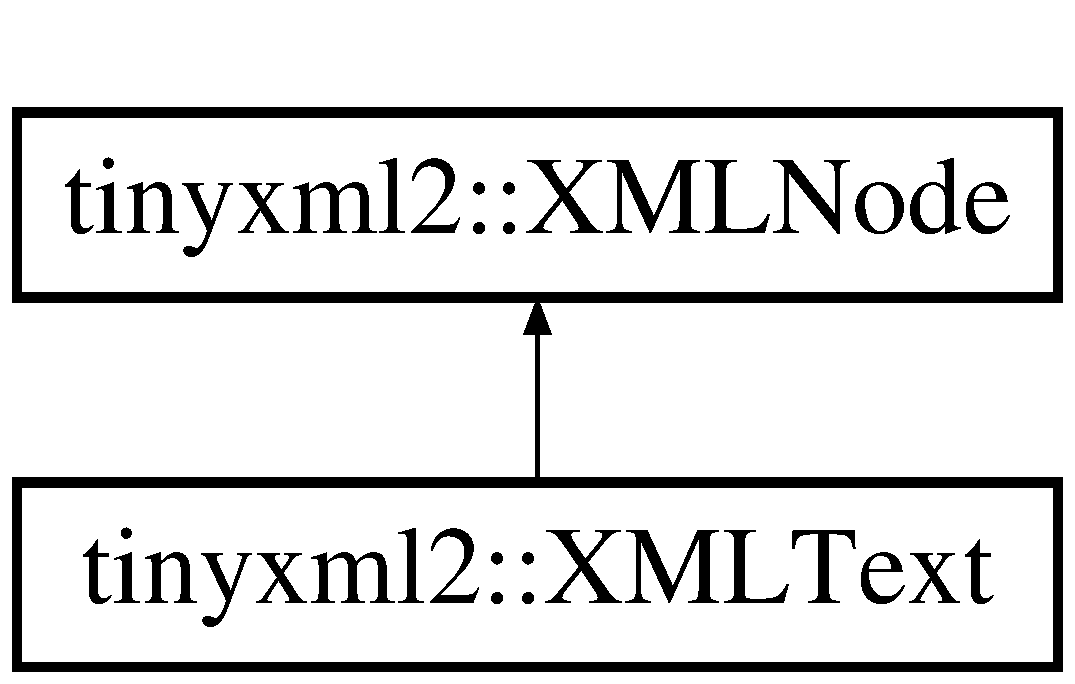
\includegraphics[height=2.000000cm]{classtinyxml2_1_1_x_m_l_text}
\end{center}
\end{figure}
\subsection*{Public Member Functions}
\begin{DoxyCompactItemize}
\item 
virtual bool \hyperlink{classtinyxml2_1_1_x_m_l_text_ae659d4fc7351a7df11c111cbe1ade46f}{Accept} (\hyperlink{classtinyxml2_1_1_x_m_l_visitor}{X\+M\+L\+Visitor} $\ast$visitor) const 
\item 
virtual \hyperlink{classtinyxml2_1_1_x_m_l_text}{X\+M\+L\+Text} $\ast$ \hyperlink{classtinyxml2_1_1_x_m_l_text_ab1213b4ddebe9b17ec7e7040e9f1caf7}{To\+Text} ()
\begin{DoxyCompactList}\small\item\em Safely cast to Text, or null. \end{DoxyCompactList}\item 
virtual const \hyperlink{classtinyxml2_1_1_x_m_l_text}{X\+M\+L\+Text} $\ast$ \hyperlink{classtinyxml2_1_1_x_m_l_text_a1e53cbc60968fe966790a65eaf87baaa}{To\+Text} () const 
\item 
void \hyperlink{classtinyxml2_1_1_x_m_l_text_ad080357d76ab7cc59d7651249949329d}{Set\+C\+Data} (bool is\+C\+Data)
\begin{DoxyCompactList}\small\item\em Declare whether this should be C\+D\+A\+T\+A or standard text. \end{DoxyCompactList}\item 
bool \hyperlink{classtinyxml2_1_1_x_m_l_text_a125574fe49da80efbae1349f20d02d41}{C\+Data} () const 
\begin{DoxyCompactList}\small\item\em Returns true if this is a C\+D\+A\+T\+A text element. \end{DoxyCompactList}\item 
char $\ast$ \hyperlink{classtinyxml2_1_1_x_m_l_text_ac18d9eec9f12b827b0d02b0847bf279e}{Parse\+Deep} (char $\ast$, \hyperlink{classtinyxml2_1_1_str_pair}{Str\+Pair} $\ast$end\+Tag)
\item 
virtual \hyperlink{classtinyxml2_1_1_x_m_l_node}{X\+M\+L\+Node} $\ast$ \hyperlink{classtinyxml2_1_1_x_m_l_text_af5115f8cc83de2947ed6a9d13e2f88c8}{Shallow\+Clone} (\hyperlink{classtinyxml2_1_1_x_m_l_document}{X\+M\+L\+Document} $\ast$document) const 
\item 
virtual bool \hyperlink{classtinyxml2_1_1_x_m_l_text_a1588aa5d23cb21eb31f36df0aaaa8d66}{Shallow\+Equal} (const \hyperlink{classtinyxml2_1_1_x_m_l_node}{X\+M\+L\+Node} $\ast$compare) const 
\end{DoxyCompactItemize}
\subsection*{Protected Member Functions}
\begin{DoxyCompactItemize}
\item 
\hyperlink{classtinyxml2_1_1_x_m_l_text_ad9f46d70e61e5386ead93728d8b90267}{X\+M\+L\+Text} (\hyperlink{classtinyxml2_1_1_x_m_l_document}{X\+M\+L\+Document} $\ast$doc)
\item 
virtual \hyperlink{classtinyxml2_1_1_x_m_l_text_ae9b8790d0dc13914394dbd7437c0e59d}{$\sim$\+X\+M\+L\+Text} ()
\end{DoxyCompactItemize}
\subsection*{Friends}
\begin{DoxyCompactItemize}
\item 
class \hyperlink{classtinyxml2_1_1_x_m_l_text_a449202cfc89e7ae5c2f81995476f9ec1}{X\+M\+L\+Base}
\item 
class \hyperlink{classtinyxml2_1_1_x_m_l_text_a4eee3bda60c60a30e4e8cd4ea91c4c6e}{X\+M\+L\+Document}
\end{DoxyCompactItemize}
\subsection*{Additional Inherited Members}


\subsection{Detailed Description}
X\+M\+L text.

Note that a text node can have child element nodes, for example\+: \begin{DoxyVerb}<root>This is <b>bold</b></root>
\end{DoxyVerb}


A text node can have 2 ways to output the next. \char`\"{}normal\char`\"{} output and C\+D\+A\+T\+A. It will default to the mode it was parsed from the X\+M\+L file and you generally want to leave it alone, but you can change the output mode with \hyperlink{classtinyxml2_1_1_x_m_l_text_ad080357d76ab7cc59d7651249949329d}{Set\+C\+Data()} and query it with \hyperlink{classtinyxml2_1_1_x_m_l_text_a125574fe49da80efbae1349f20d02d41}{C\+Data()}. 

\subsection{Constructor \& Destructor Documentation}
\hypertarget{classtinyxml2_1_1_x_m_l_text_ad9f46d70e61e5386ead93728d8b90267}{}\index{tinyxml2\+::\+X\+M\+L\+Text@{tinyxml2\+::\+X\+M\+L\+Text}!X\+M\+L\+Text@{X\+M\+L\+Text}}
\index{X\+M\+L\+Text@{X\+M\+L\+Text}!tinyxml2\+::\+X\+M\+L\+Text@{tinyxml2\+::\+X\+M\+L\+Text}}
\subsubsection[{X\+M\+L\+Text}]{\setlength{\rightskip}{0pt plus 5cm}tinyxml2\+::\+X\+M\+L\+Text\+::\+X\+M\+L\+Text (
\begin{DoxyParamCaption}
\item[{{\bf X\+M\+L\+Document} $\ast$}]{doc}
\end{DoxyParamCaption}
)\hspace{0.3cm}{\ttfamily [inline]}, {\ttfamily [protected]}}\label{classtinyxml2_1_1_x_m_l_text_ad9f46d70e61e5386ead93728d8b90267}
\hypertarget{classtinyxml2_1_1_x_m_l_text_ae9b8790d0dc13914394dbd7437c0e59d}{}\index{tinyxml2\+::\+X\+M\+L\+Text@{tinyxml2\+::\+X\+M\+L\+Text}!````~X\+M\+L\+Text@{$\sim$\+X\+M\+L\+Text}}
\index{````~X\+M\+L\+Text@{$\sim$\+X\+M\+L\+Text}!tinyxml2\+::\+X\+M\+L\+Text@{tinyxml2\+::\+X\+M\+L\+Text}}
\subsubsection[{$\sim$\+X\+M\+L\+Text}]{\setlength{\rightskip}{0pt plus 5cm}virtual tinyxml2\+::\+X\+M\+L\+Text\+::$\sim$\+X\+M\+L\+Text (
\begin{DoxyParamCaption}
{}
\end{DoxyParamCaption}
)\hspace{0.3cm}{\ttfamily [inline]}, {\ttfamily [protected]}, {\ttfamily [virtual]}}\label{classtinyxml2_1_1_x_m_l_text_ae9b8790d0dc13914394dbd7437c0e59d}


\subsection{Member Function Documentation}
\hypertarget{classtinyxml2_1_1_x_m_l_text_ae659d4fc7351a7df11c111cbe1ade46f}{}\index{tinyxml2\+::\+X\+M\+L\+Text@{tinyxml2\+::\+X\+M\+L\+Text}!Accept@{Accept}}
\index{Accept@{Accept}!tinyxml2\+::\+X\+M\+L\+Text@{tinyxml2\+::\+X\+M\+L\+Text}}
\subsubsection[{Accept}]{\setlength{\rightskip}{0pt plus 5cm}bool tinyxml2\+::\+X\+M\+L\+Text\+::\+Accept (
\begin{DoxyParamCaption}
\item[{{\bf X\+M\+L\+Visitor} $\ast$}]{visitor}
\end{DoxyParamCaption}
) const\hspace{0.3cm}{\ttfamily [virtual]}}\label{classtinyxml2_1_1_x_m_l_text_ae659d4fc7351a7df11c111cbe1ade46f}
Accept a hierarchical visit of the nodes in the Tiny\+X\+M\+L-\/2 D\+O\+M. Every node in the X\+M\+L tree will be conditionally visited and the host will be called back via the \hyperlink{classtinyxml2_1_1_x_m_l_visitor}{X\+M\+L\+Visitor} interface.

This is essentially a S\+A\+X interface for Tiny\+X\+M\+L-\/2. (Note however it doesn\textquotesingle{}t re-\/parse the X\+M\+L for the callbacks, so the performance of Tiny\+X\+M\+L-\/2 is unchanged by using this interface versus any other.)

The interface has been based on ideas from\+:


\begin{DoxyItemize}
\item \href{http://www.saxproject.org/}{\tt http\+://www.\+saxproject.\+org/}
\item \href{http://c2.com/cgi/wiki?HierarchicalVisitorPattern}{\tt http\+://c2.\+com/cgi/wiki?\+Hierarchical\+Visitor\+Pattern}
\end{DoxyItemize}

Which are both good references for \char`\"{}visiting\char`\"{}.

An example of using \hyperlink{classtinyxml2_1_1_x_m_l_text_ae659d4fc7351a7df11c111cbe1ade46f}{Accept()}\+: \begin{DoxyVerb}XMLPrinter printer;
tinyxmlDoc.Accept( &printer );
const char* xmlcstr = printer.CStr();
\end{DoxyVerb}
 

Implements \hyperlink{classtinyxml2_1_1_x_m_l_node_a81e66df0a44c67a7af17f3b77a152785}{tinyxml2\+::\+X\+M\+L\+Node}.

\hypertarget{classtinyxml2_1_1_x_m_l_text_a125574fe49da80efbae1349f20d02d41}{}\index{tinyxml2\+::\+X\+M\+L\+Text@{tinyxml2\+::\+X\+M\+L\+Text}!C\+Data@{C\+Data}}
\index{C\+Data@{C\+Data}!tinyxml2\+::\+X\+M\+L\+Text@{tinyxml2\+::\+X\+M\+L\+Text}}
\subsubsection[{C\+Data}]{\setlength{\rightskip}{0pt plus 5cm}bool tinyxml2\+::\+X\+M\+L\+Text\+::\+C\+Data (
\begin{DoxyParamCaption}
{}
\end{DoxyParamCaption}
) const\hspace{0.3cm}{\ttfamily [inline]}}\label{classtinyxml2_1_1_x_m_l_text_a125574fe49da80efbae1349f20d02d41}


Returns true if this is a C\+D\+A\+T\+A text element. 

\hypertarget{classtinyxml2_1_1_x_m_l_text_ac18d9eec9f12b827b0d02b0847bf279e}{}\index{tinyxml2\+::\+X\+M\+L\+Text@{tinyxml2\+::\+X\+M\+L\+Text}!Parse\+Deep@{Parse\+Deep}}
\index{Parse\+Deep@{Parse\+Deep}!tinyxml2\+::\+X\+M\+L\+Text@{tinyxml2\+::\+X\+M\+L\+Text}}
\subsubsection[{Parse\+Deep}]{\setlength{\rightskip}{0pt plus 5cm}char $\ast$ tinyxml2\+::\+X\+M\+L\+Text\+::\+Parse\+Deep (
\begin{DoxyParamCaption}
\item[{char $\ast$}]{p, }
\item[{{\bf Str\+Pair} $\ast$}]{end\+Tag}
\end{DoxyParamCaption}
)\hspace{0.3cm}{\ttfamily [virtual]}}\label{classtinyxml2_1_1_x_m_l_text_ac18d9eec9f12b827b0d02b0847bf279e}


Reimplemented from \hyperlink{classtinyxml2_1_1_x_m_l_node_a7610d0f603e8b603d2078521811a23c1}{tinyxml2\+::\+X\+M\+L\+Node}.

\hypertarget{classtinyxml2_1_1_x_m_l_text_ad080357d76ab7cc59d7651249949329d}{}\index{tinyxml2\+::\+X\+M\+L\+Text@{tinyxml2\+::\+X\+M\+L\+Text}!Set\+C\+Data@{Set\+C\+Data}}
\index{Set\+C\+Data@{Set\+C\+Data}!tinyxml2\+::\+X\+M\+L\+Text@{tinyxml2\+::\+X\+M\+L\+Text}}
\subsubsection[{Set\+C\+Data}]{\setlength{\rightskip}{0pt plus 5cm}void tinyxml2\+::\+X\+M\+L\+Text\+::\+Set\+C\+Data (
\begin{DoxyParamCaption}
\item[{bool}]{is\+C\+Data}
\end{DoxyParamCaption}
)\hspace{0.3cm}{\ttfamily [inline]}}\label{classtinyxml2_1_1_x_m_l_text_ad080357d76ab7cc59d7651249949329d}


Declare whether this should be C\+D\+A\+T\+A or standard text. 

\hypertarget{classtinyxml2_1_1_x_m_l_text_af5115f8cc83de2947ed6a9d13e2f88c8}{}\index{tinyxml2\+::\+X\+M\+L\+Text@{tinyxml2\+::\+X\+M\+L\+Text}!Shallow\+Clone@{Shallow\+Clone}}
\index{Shallow\+Clone@{Shallow\+Clone}!tinyxml2\+::\+X\+M\+L\+Text@{tinyxml2\+::\+X\+M\+L\+Text}}
\subsubsection[{Shallow\+Clone}]{\setlength{\rightskip}{0pt plus 5cm}{\bf X\+M\+L\+Node} $\ast$ tinyxml2\+::\+X\+M\+L\+Text\+::\+Shallow\+Clone (
\begin{DoxyParamCaption}
\item[{{\bf X\+M\+L\+Document} $\ast$}]{document}
\end{DoxyParamCaption}
) const\hspace{0.3cm}{\ttfamily [virtual]}}\label{classtinyxml2_1_1_x_m_l_text_af5115f8cc83de2947ed6a9d13e2f88c8}
Make a copy of this node, but not its children. You may pass in a Document pointer that will be the owner of the new Node. If the \textquotesingle{}document\textquotesingle{} is null, then the node returned will be allocated from the current Document. (this-\/$>$\hyperlink{classtinyxml2_1_1_x_m_l_node_af343d1ef0b45c0020e62d784d7e67a68}{Get\+Document()})

Note\+: if called on a \hyperlink{classtinyxml2_1_1_x_m_l_document}{X\+M\+L\+Document}, this will return null. 

Implements \hyperlink{classtinyxml2_1_1_x_m_l_node_a8402cbd3129d20e9e6024bbcc0531283}{tinyxml2\+::\+X\+M\+L\+Node}.

\hypertarget{classtinyxml2_1_1_x_m_l_text_a1588aa5d23cb21eb31f36df0aaaa8d66}{}\index{tinyxml2\+::\+X\+M\+L\+Text@{tinyxml2\+::\+X\+M\+L\+Text}!Shallow\+Equal@{Shallow\+Equal}}
\index{Shallow\+Equal@{Shallow\+Equal}!tinyxml2\+::\+X\+M\+L\+Text@{tinyxml2\+::\+X\+M\+L\+Text}}
\subsubsection[{Shallow\+Equal}]{\setlength{\rightskip}{0pt plus 5cm}bool tinyxml2\+::\+X\+M\+L\+Text\+::\+Shallow\+Equal (
\begin{DoxyParamCaption}
\item[{const {\bf X\+M\+L\+Node} $\ast$}]{compare}
\end{DoxyParamCaption}
) const\hspace{0.3cm}{\ttfamily [virtual]}}\label{classtinyxml2_1_1_x_m_l_text_a1588aa5d23cb21eb31f36df0aaaa8d66}
Test if 2 nodes are the same, but don\textquotesingle{}t test children. The 2 nodes do not need to be in the same Document.

Note\+: if called on a \hyperlink{classtinyxml2_1_1_x_m_l_document}{X\+M\+L\+Document}, this will return false. 

Implements \hyperlink{classtinyxml2_1_1_x_m_l_node_a7ce18b751c3ea09eac292dca264f9226}{tinyxml2\+::\+X\+M\+L\+Node}.

\hypertarget{classtinyxml2_1_1_x_m_l_text_ab1213b4ddebe9b17ec7e7040e9f1caf7}{}\index{tinyxml2\+::\+X\+M\+L\+Text@{tinyxml2\+::\+X\+M\+L\+Text}!To\+Text@{To\+Text}}
\index{To\+Text@{To\+Text}!tinyxml2\+::\+X\+M\+L\+Text@{tinyxml2\+::\+X\+M\+L\+Text}}
\subsubsection[{To\+Text}]{\setlength{\rightskip}{0pt plus 5cm}virtual {\bf X\+M\+L\+Text}$\ast$ tinyxml2\+::\+X\+M\+L\+Text\+::\+To\+Text (
\begin{DoxyParamCaption}
{}
\end{DoxyParamCaption}
)\hspace{0.3cm}{\ttfamily [inline]}, {\ttfamily [virtual]}}\label{classtinyxml2_1_1_x_m_l_text_ab1213b4ddebe9b17ec7e7040e9f1caf7}


Safely cast to Text, or null. 



Reimplemented from \hyperlink{classtinyxml2_1_1_x_m_l_node_a41c55dab9162d1eb62db2008430e376b}{tinyxml2\+::\+X\+M\+L\+Node}.

\hypertarget{classtinyxml2_1_1_x_m_l_text_a1e53cbc60968fe966790a65eaf87baaa}{}\index{tinyxml2\+::\+X\+M\+L\+Text@{tinyxml2\+::\+X\+M\+L\+Text}!To\+Text@{To\+Text}}
\index{To\+Text@{To\+Text}!tinyxml2\+::\+X\+M\+L\+Text@{tinyxml2\+::\+X\+M\+L\+Text}}
\subsubsection[{To\+Text}]{\setlength{\rightskip}{0pt plus 5cm}virtual const {\bf X\+M\+L\+Text}$\ast$ tinyxml2\+::\+X\+M\+L\+Text\+::\+To\+Text (
\begin{DoxyParamCaption}
{}
\end{DoxyParamCaption}
) const\hspace{0.3cm}{\ttfamily [inline]}, {\ttfamily [virtual]}}\label{classtinyxml2_1_1_x_m_l_text_a1e53cbc60968fe966790a65eaf87baaa}


Reimplemented from \hyperlink{classtinyxml2_1_1_x_m_l_node_a89009ffc1b9f5d692bf8d4c9f18c3bec}{tinyxml2\+::\+X\+M\+L\+Node}.



\subsection{Friends And Related Function Documentation}
\hypertarget{classtinyxml2_1_1_x_m_l_text_a449202cfc89e7ae5c2f81995476f9ec1}{}\index{tinyxml2\+::\+X\+M\+L\+Text@{tinyxml2\+::\+X\+M\+L\+Text}!X\+M\+L\+Base@{X\+M\+L\+Base}}
\index{X\+M\+L\+Base@{X\+M\+L\+Base}!tinyxml2\+::\+X\+M\+L\+Text@{tinyxml2\+::\+X\+M\+L\+Text}}
\subsubsection[{X\+M\+L\+Base}]{\setlength{\rightskip}{0pt plus 5cm}friend class X\+M\+L\+Base\hspace{0.3cm}{\ttfamily [friend]}}\label{classtinyxml2_1_1_x_m_l_text_a449202cfc89e7ae5c2f81995476f9ec1}
\hypertarget{classtinyxml2_1_1_x_m_l_text_a4eee3bda60c60a30e4e8cd4ea91c4c6e}{}\index{tinyxml2\+::\+X\+M\+L\+Text@{tinyxml2\+::\+X\+M\+L\+Text}!X\+M\+L\+Document@{X\+M\+L\+Document}}
\index{X\+M\+L\+Document@{X\+M\+L\+Document}!tinyxml2\+::\+X\+M\+L\+Text@{tinyxml2\+::\+X\+M\+L\+Text}}
\subsubsection[{X\+M\+L\+Document}]{\setlength{\rightskip}{0pt plus 5cm}friend class {\bf X\+M\+L\+Document}\hspace{0.3cm}{\ttfamily [friend]}}\label{classtinyxml2_1_1_x_m_l_text_a4eee3bda60c60a30e4e8cd4ea91c4c6e}


The documentation for this class was generated from the following files\+:\begin{DoxyCompactItemize}
\item 
\hyperlink{tinyxml2_8h}{tinyxml2.\+h}\item 
\hyperlink{tinyxml2_8cpp}{tinyxml2.\+cpp}\end{DoxyCompactItemize}

\hypertarget{classtinyxml2_1_1_x_m_l_unknown}{}\section{tinyxml2\+:\+:X\+M\+L\+Unknown Class Reference}
\label{classtinyxml2_1_1_x_m_l_unknown}\index{tinyxml2\+::\+X\+M\+L\+Unknown@{tinyxml2\+::\+X\+M\+L\+Unknown}}


{\ttfamily \#include $<$tinyxml2.\+h$>$}

Inheritance diagram for tinyxml2\+:\+:X\+M\+L\+Unknown\+:\begin{figure}[H]
\begin{center}
\leavevmode
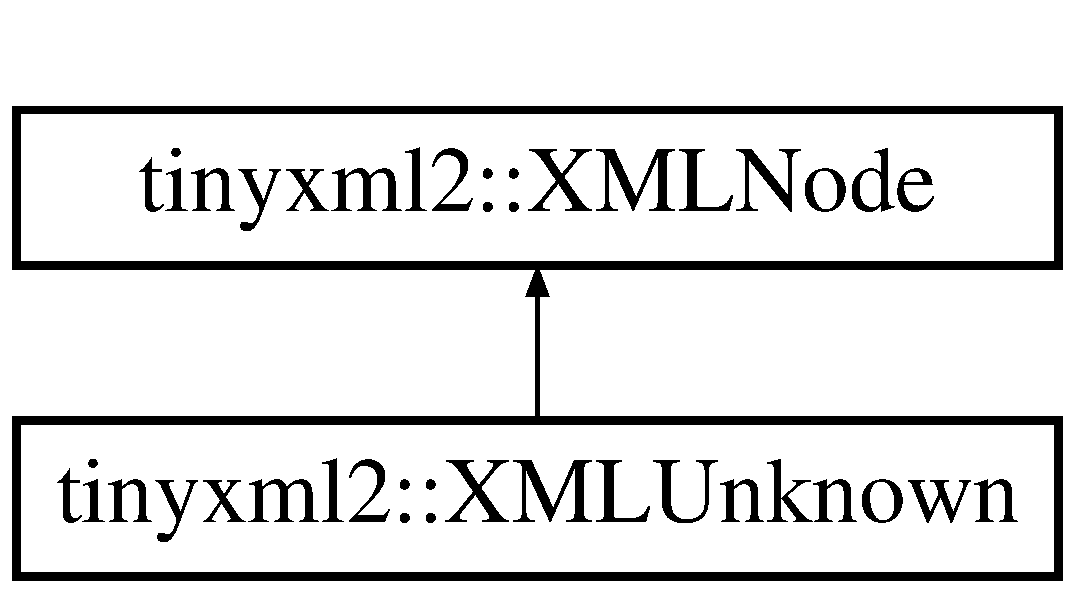
\includegraphics[height=2.000000cm]{classtinyxml2_1_1_x_m_l_unknown}
\end{center}
\end{figure}
\subsection*{Public Member Functions}
\begin{DoxyCompactItemize}
\item 
virtual \hyperlink{classtinyxml2_1_1_x_m_l_unknown}{X\+M\+L\+Unknown} $\ast$ \hyperlink{classtinyxml2_1_1_x_m_l_unknown_af4374856421921cad578c8affae872b6}{To\+Unknown} ()
\begin{DoxyCompactList}\small\item\em Safely cast to an Unknown, or null. \end{DoxyCompactList}\item 
virtual const \hyperlink{classtinyxml2_1_1_x_m_l_unknown}{X\+M\+L\+Unknown} $\ast$ \hyperlink{classtinyxml2_1_1_x_m_l_unknown_a257987e79955399e6e9f119b58d4bb30}{To\+Unknown} () const 
\item 
virtual bool \hyperlink{classtinyxml2_1_1_x_m_l_unknown_a0d341ab804a1438a474810bb5bd29dd5}{Accept} (\hyperlink{classtinyxml2_1_1_x_m_l_visitor}{X\+M\+L\+Visitor} $\ast$visitor) const 
\item 
char $\ast$ \hyperlink{classtinyxml2_1_1_x_m_l_unknown_a0e4f3509dee42a4d45a7f0002be568cc}{Parse\+Deep} (char $\ast$, \hyperlink{classtinyxml2_1_1_str_pair}{Str\+Pair} $\ast$end\+Tag)
\item 
virtual \hyperlink{classtinyxml2_1_1_x_m_l_node}{X\+M\+L\+Node} $\ast$ \hyperlink{classtinyxml2_1_1_x_m_l_unknown_aa09fc7cb0cd64d6bb9c5ae00ffc549ec}{Shallow\+Clone} (\hyperlink{classtinyxml2_1_1_x_m_l_document}{X\+M\+L\+Document} $\ast$document) const 
\item 
virtual bool \hyperlink{classtinyxml2_1_1_x_m_l_unknown_a0169df157bf69a092b404ca49621ff1a}{Shallow\+Equal} (const \hyperlink{classtinyxml2_1_1_x_m_l_node}{X\+M\+L\+Node} $\ast$compare) const 
\end{DoxyCompactItemize}
\subsection*{Protected Member Functions}
\begin{DoxyCompactItemize}
\item 
\hyperlink{classtinyxml2_1_1_x_m_l_unknown_a9391eb679598d50baba424e6f1aa367b}{X\+M\+L\+Unknown} (\hyperlink{classtinyxml2_1_1_x_m_l_document}{X\+M\+L\+Document} $\ast$doc)
\item 
virtual \hyperlink{classtinyxml2_1_1_x_m_l_unknown_a86fcd722ca173a7f385bafafa879f26e}{$\sim$\+X\+M\+L\+Unknown} ()
\end{DoxyCompactItemize}
\subsection*{Friends}
\begin{DoxyCompactItemize}
\item 
class \hyperlink{classtinyxml2_1_1_x_m_l_unknown_a4eee3bda60c60a30e4e8cd4ea91c4c6e}{X\+M\+L\+Document}
\end{DoxyCompactItemize}
\subsection*{Additional Inherited Members}


\subsection{Detailed Description}
Any tag that Tiny\+X\+M\+L-\/2 doesn\textquotesingle{}t recognize is saved as an unknown. It is a tag of text, but should not be modified. It will be written back to the X\+M\+L, unchanged, when the file is saved.

D\+T\+D tags get thrown into X\+M\+L\+Unknowns. 

\subsection{Constructor \& Destructor Documentation}
\hypertarget{classtinyxml2_1_1_x_m_l_unknown_a9391eb679598d50baba424e6f1aa367b}{}\index{tinyxml2\+::\+X\+M\+L\+Unknown@{tinyxml2\+::\+X\+M\+L\+Unknown}!X\+M\+L\+Unknown@{X\+M\+L\+Unknown}}
\index{X\+M\+L\+Unknown@{X\+M\+L\+Unknown}!tinyxml2\+::\+X\+M\+L\+Unknown@{tinyxml2\+::\+X\+M\+L\+Unknown}}
\subsubsection[{X\+M\+L\+Unknown}]{\setlength{\rightskip}{0pt plus 5cm}tinyxml2\+::\+X\+M\+L\+Unknown\+::\+X\+M\+L\+Unknown (
\begin{DoxyParamCaption}
\item[{{\bf X\+M\+L\+Document} $\ast$}]{doc}
\end{DoxyParamCaption}
)\hspace{0.3cm}{\ttfamily [protected]}}\label{classtinyxml2_1_1_x_m_l_unknown_a9391eb679598d50baba424e6f1aa367b}
\hypertarget{classtinyxml2_1_1_x_m_l_unknown_a86fcd722ca173a7f385bafafa879f26e}{}\index{tinyxml2\+::\+X\+M\+L\+Unknown@{tinyxml2\+::\+X\+M\+L\+Unknown}!````~X\+M\+L\+Unknown@{$\sim$\+X\+M\+L\+Unknown}}
\index{````~X\+M\+L\+Unknown@{$\sim$\+X\+M\+L\+Unknown}!tinyxml2\+::\+X\+M\+L\+Unknown@{tinyxml2\+::\+X\+M\+L\+Unknown}}
\subsubsection[{$\sim$\+X\+M\+L\+Unknown}]{\setlength{\rightskip}{0pt plus 5cm}tinyxml2\+::\+X\+M\+L\+Unknown\+::$\sim$\+X\+M\+L\+Unknown (
\begin{DoxyParamCaption}
{}
\end{DoxyParamCaption}
)\hspace{0.3cm}{\ttfamily [protected]}, {\ttfamily [virtual]}}\label{classtinyxml2_1_1_x_m_l_unknown_a86fcd722ca173a7f385bafafa879f26e}


\subsection{Member Function Documentation}
\hypertarget{classtinyxml2_1_1_x_m_l_unknown_a0d341ab804a1438a474810bb5bd29dd5}{}\index{tinyxml2\+::\+X\+M\+L\+Unknown@{tinyxml2\+::\+X\+M\+L\+Unknown}!Accept@{Accept}}
\index{Accept@{Accept}!tinyxml2\+::\+X\+M\+L\+Unknown@{tinyxml2\+::\+X\+M\+L\+Unknown}}
\subsubsection[{Accept}]{\setlength{\rightskip}{0pt plus 5cm}bool tinyxml2\+::\+X\+M\+L\+Unknown\+::\+Accept (
\begin{DoxyParamCaption}
\item[{{\bf X\+M\+L\+Visitor} $\ast$}]{visitor}
\end{DoxyParamCaption}
) const\hspace{0.3cm}{\ttfamily [virtual]}}\label{classtinyxml2_1_1_x_m_l_unknown_a0d341ab804a1438a474810bb5bd29dd5}
Accept a hierarchical visit of the nodes in the Tiny\+X\+M\+L-\/2 D\+O\+M. Every node in the X\+M\+L tree will be conditionally visited and the host will be called back via the \hyperlink{classtinyxml2_1_1_x_m_l_visitor}{X\+M\+L\+Visitor} interface.

This is essentially a S\+A\+X interface for Tiny\+X\+M\+L-\/2. (Note however it doesn\textquotesingle{}t re-\/parse the X\+M\+L for the callbacks, so the performance of Tiny\+X\+M\+L-\/2 is unchanged by using this interface versus any other.)

The interface has been based on ideas from\+:


\begin{DoxyItemize}
\item \href{http://www.saxproject.org/}{\tt http\+://www.\+saxproject.\+org/}
\item \href{http://c2.com/cgi/wiki?HierarchicalVisitorPattern}{\tt http\+://c2.\+com/cgi/wiki?\+Hierarchical\+Visitor\+Pattern}
\end{DoxyItemize}

Which are both good references for \char`\"{}visiting\char`\"{}.

An example of using \hyperlink{classtinyxml2_1_1_x_m_l_unknown_a0d341ab804a1438a474810bb5bd29dd5}{Accept()}\+: \begin{DoxyVerb}XMLPrinter printer;
tinyxmlDoc.Accept( &printer );
const char* xmlcstr = printer.CStr();
\end{DoxyVerb}
 

Implements \hyperlink{classtinyxml2_1_1_x_m_l_node_a81e66df0a44c67a7af17f3b77a152785}{tinyxml2\+::\+X\+M\+L\+Node}.

\hypertarget{classtinyxml2_1_1_x_m_l_unknown_a0e4f3509dee42a4d45a7f0002be568cc}{}\index{tinyxml2\+::\+X\+M\+L\+Unknown@{tinyxml2\+::\+X\+M\+L\+Unknown}!Parse\+Deep@{Parse\+Deep}}
\index{Parse\+Deep@{Parse\+Deep}!tinyxml2\+::\+X\+M\+L\+Unknown@{tinyxml2\+::\+X\+M\+L\+Unknown}}
\subsubsection[{Parse\+Deep}]{\setlength{\rightskip}{0pt plus 5cm}char $\ast$ tinyxml2\+::\+X\+M\+L\+Unknown\+::\+Parse\+Deep (
\begin{DoxyParamCaption}
\item[{char $\ast$}]{p, }
\item[{{\bf Str\+Pair} $\ast$}]{end\+Tag}
\end{DoxyParamCaption}
)\hspace{0.3cm}{\ttfamily [virtual]}}\label{classtinyxml2_1_1_x_m_l_unknown_a0e4f3509dee42a4d45a7f0002be568cc}


Reimplemented from \hyperlink{classtinyxml2_1_1_x_m_l_node_a7610d0f603e8b603d2078521811a23c1}{tinyxml2\+::\+X\+M\+L\+Node}.

\hypertarget{classtinyxml2_1_1_x_m_l_unknown_aa09fc7cb0cd64d6bb9c5ae00ffc549ec}{}\index{tinyxml2\+::\+X\+M\+L\+Unknown@{tinyxml2\+::\+X\+M\+L\+Unknown}!Shallow\+Clone@{Shallow\+Clone}}
\index{Shallow\+Clone@{Shallow\+Clone}!tinyxml2\+::\+X\+M\+L\+Unknown@{tinyxml2\+::\+X\+M\+L\+Unknown}}
\subsubsection[{Shallow\+Clone}]{\setlength{\rightskip}{0pt plus 5cm}{\bf X\+M\+L\+Node} $\ast$ tinyxml2\+::\+X\+M\+L\+Unknown\+::\+Shallow\+Clone (
\begin{DoxyParamCaption}
\item[{{\bf X\+M\+L\+Document} $\ast$}]{document}
\end{DoxyParamCaption}
) const\hspace{0.3cm}{\ttfamily [virtual]}}\label{classtinyxml2_1_1_x_m_l_unknown_aa09fc7cb0cd64d6bb9c5ae00ffc549ec}
Make a copy of this node, but not its children. You may pass in a Document pointer that will be the owner of the new Node. If the \textquotesingle{}document\textquotesingle{} is null, then the node returned will be allocated from the current Document. (this-\/$>$\hyperlink{classtinyxml2_1_1_x_m_l_node_af343d1ef0b45c0020e62d784d7e67a68}{Get\+Document()})

Note\+: if called on a \hyperlink{classtinyxml2_1_1_x_m_l_document}{X\+M\+L\+Document}, this will return null. 

Implements \hyperlink{classtinyxml2_1_1_x_m_l_node_a8402cbd3129d20e9e6024bbcc0531283}{tinyxml2\+::\+X\+M\+L\+Node}.

\hypertarget{classtinyxml2_1_1_x_m_l_unknown_a0169df157bf69a092b404ca49621ff1a}{}\index{tinyxml2\+::\+X\+M\+L\+Unknown@{tinyxml2\+::\+X\+M\+L\+Unknown}!Shallow\+Equal@{Shallow\+Equal}}
\index{Shallow\+Equal@{Shallow\+Equal}!tinyxml2\+::\+X\+M\+L\+Unknown@{tinyxml2\+::\+X\+M\+L\+Unknown}}
\subsubsection[{Shallow\+Equal}]{\setlength{\rightskip}{0pt plus 5cm}bool tinyxml2\+::\+X\+M\+L\+Unknown\+::\+Shallow\+Equal (
\begin{DoxyParamCaption}
\item[{const {\bf X\+M\+L\+Node} $\ast$}]{compare}
\end{DoxyParamCaption}
) const\hspace{0.3cm}{\ttfamily [virtual]}}\label{classtinyxml2_1_1_x_m_l_unknown_a0169df157bf69a092b404ca49621ff1a}
Test if 2 nodes are the same, but don\textquotesingle{}t test children. The 2 nodes do not need to be in the same Document.

Note\+: if called on a \hyperlink{classtinyxml2_1_1_x_m_l_document}{X\+M\+L\+Document}, this will return false. 

Implements \hyperlink{classtinyxml2_1_1_x_m_l_node_a7ce18b751c3ea09eac292dca264f9226}{tinyxml2\+::\+X\+M\+L\+Node}.

\hypertarget{classtinyxml2_1_1_x_m_l_unknown_af4374856421921cad578c8affae872b6}{}\index{tinyxml2\+::\+X\+M\+L\+Unknown@{tinyxml2\+::\+X\+M\+L\+Unknown}!To\+Unknown@{To\+Unknown}}
\index{To\+Unknown@{To\+Unknown}!tinyxml2\+::\+X\+M\+L\+Unknown@{tinyxml2\+::\+X\+M\+L\+Unknown}}
\subsubsection[{To\+Unknown}]{\setlength{\rightskip}{0pt plus 5cm}virtual {\bf X\+M\+L\+Unknown}$\ast$ tinyxml2\+::\+X\+M\+L\+Unknown\+::\+To\+Unknown (
\begin{DoxyParamCaption}
{}
\end{DoxyParamCaption}
)\hspace{0.3cm}{\ttfamily [inline]}, {\ttfamily [virtual]}}\label{classtinyxml2_1_1_x_m_l_unknown_af4374856421921cad578c8affae872b6}


Safely cast to an Unknown, or null. 



Reimplemented from \hyperlink{classtinyxml2_1_1_x_m_l_node_a8675a74aa0ada6eccab0c77ef3e5b9bd}{tinyxml2\+::\+X\+M\+L\+Node}.

\hypertarget{classtinyxml2_1_1_x_m_l_unknown_a257987e79955399e6e9f119b58d4bb30}{}\index{tinyxml2\+::\+X\+M\+L\+Unknown@{tinyxml2\+::\+X\+M\+L\+Unknown}!To\+Unknown@{To\+Unknown}}
\index{To\+Unknown@{To\+Unknown}!tinyxml2\+::\+X\+M\+L\+Unknown@{tinyxml2\+::\+X\+M\+L\+Unknown}}
\subsubsection[{To\+Unknown}]{\setlength{\rightskip}{0pt plus 5cm}virtual const {\bf X\+M\+L\+Unknown}$\ast$ tinyxml2\+::\+X\+M\+L\+Unknown\+::\+To\+Unknown (
\begin{DoxyParamCaption}
{}
\end{DoxyParamCaption}
) const\hspace{0.3cm}{\ttfamily [inline]}, {\ttfamily [virtual]}}\label{classtinyxml2_1_1_x_m_l_unknown_a257987e79955399e6e9f119b58d4bb30}


Reimplemented from \hyperlink{classtinyxml2_1_1_x_m_l_node_a71f5ae90296dbe67979f83fe97073efa}{tinyxml2\+::\+X\+M\+L\+Node}.



\subsection{Friends And Related Function Documentation}
\hypertarget{classtinyxml2_1_1_x_m_l_unknown_a4eee3bda60c60a30e4e8cd4ea91c4c6e}{}\index{tinyxml2\+::\+X\+M\+L\+Unknown@{tinyxml2\+::\+X\+M\+L\+Unknown}!X\+M\+L\+Document@{X\+M\+L\+Document}}
\index{X\+M\+L\+Document@{X\+M\+L\+Document}!tinyxml2\+::\+X\+M\+L\+Unknown@{tinyxml2\+::\+X\+M\+L\+Unknown}}
\subsubsection[{X\+M\+L\+Document}]{\setlength{\rightskip}{0pt plus 5cm}friend class {\bf X\+M\+L\+Document}\hspace{0.3cm}{\ttfamily [friend]}}\label{classtinyxml2_1_1_x_m_l_unknown_a4eee3bda60c60a30e4e8cd4ea91c4c6e}


The documentation for this class was generated from the following files\+:\begin{DoxyCompactItemize}
\item 
\hyperlink{tinyxml2_8h}{tinyxml2.\+h}\item 
\hyperlink{tinyxml2_8cpp}{tinyxml2.\+cpp}\end{DoxyCompactItemize}

\hypertarget{classtinyxml2_1_1_x_m_l_util}{}\section{tinyxml2\+:\+:X\+M\+L\+Util Class Reference}
\label{classtinyxml2_1_1_x_m_l_util}\index{tinyxml2\+::\+X\+M\+L\+Util@{tinyxml2\+::\+X\+M\+L\+Util}}


{\ttfamily \#include $<$tinyxml2.\+h$>$}

\subsection*{Static Public Member Functions}
\begin{DoxyCompactItemize}
\item 
static const char $\ast$ \hyperlink{classtinyxml2_1_1_x_m_l_util_a9333d20f2a34325b5115ca45849c4b2a}{Skip\+White\+Space} (const char $\ast$p)
\item 
static char $\ast$ \hyperlink{classtinyxml2_1_1_x_m_l_util_aa48025be8843ec5a79b65579d31bd8fc}{Skip\+White\+Space} (char $\ast$p)
\item 
static bool \hyperlink{classtinyxml2_1_1_x_m_l_util_a357ec3af8fc433d19023a815f45e8e33}{Is\+White\+Space} (char p)
\item 
static bool \hyperlink{classtinyxml2_1_1_x_m_l_util_abe106a69ac4d942a4381a4d9dfd0e0bd}{Is\+Name\+Start\+Char} (unsigned char ch)
\item 
static bool \hyperlink{classtinyxml2_1_1_x_m_l_util_a04b17341538fa11752f24b4301d19485}{Is\+Name\+Char} (unsigned char ch)
\item 
static bool \hyperlink{classtinyxml2_1_1_x_m_l_util_acfcd287cacfd2533e1bc9ea4dfb56602}{String\+Equal} (const char $\ast$p, const char $\ast$q, int n\+Char=I\+N\+T\+\_\+\+M\+A\+X)
\item 
static bool \hyperlink{classtinyxml2_1_1_x_m_l_util_a9780b5926e30fe6222e10f0e6cf5a04a}{Is\+U\+T\+F8\+Continuation} (const char p)
\item 
static const char $\ast$ \hyperlink{classtinyxml2_1_1_x_m_l_util_ae9bcb2bc3cd6475fdc644c8c17790555}{Read\+B\+O\+M} (const char $\ast$p, bool $\ast$has\+B\+O\+M)
\item 
static const char $\ast$ \hyperlink{classtinyxml2_1_1_x_m_l_util_a5a96e5144a8d693dc4bcd783d9964648}{Get\+Character\+Ref} (const char $\ast$p, char $\ast$value, int $\ast$length)
\item 
static void \hyperlink{classtinyxml2_1_1_x_m_l_util_a31c00d5c5dfb38382de1dfcaf4be3595}{Convert\+U\+T\+F32\+To\+U\+T\+F8} (unsigned long input, char $\ast$output, int $\ast$length)
\item 
static void \hyperlink{classtinyxml2_1_1_x_m_l_util_a3cd6c703d49b9d51bdf0f4ff6aa021c7}{To\+Str} (int v, char $\ast$buffer, int buffer\+Size)
\item 
static void \hyperlink{classtinyxml2_1_1_x_m_l_util_ac00c2e52c1c36dab3ff41d86a9bf60f9}{To\+Str} (unsigned v, char $\ast$buffer, int buffer\+Size)
\item 
static void \hyperlink{classtinyxml2_1_1_x_m_l_util_adba0718527ae9e80f663a71ea325cb11}{To\+Str} (bool v, char $\ast$buffer, int buffer\+Size)
\item 
static void \hyperlink{classtinyxml2_1_1_x_m_l_util_a8957ad44fee5fa02ba52d73aad4d0a31}{To\+Str} (float v, char $\ast$buffer, int buffer\+Size)
\item 
static void \hyperlink{classtinyxml2_1_1_x_m_l_util_a1cd141e50980fcddd6bf9af5de4b1db7}{To\+Str} (double v, char $\ast$buffer, int buffer\+Size)
\item 
static bool \hyperlink{classtinyxml2_1_1_x_m_l_util_ad4df4023d11ee3fca9689c49b9707323}{To\+Int} (const char $\ast$str, int $\ast$value)
\item 
static bool \hyperlink{classtinyxml2_1_1_x_m_l_util_a210c8637d5eb4ce3d4625294af0efc2f}{To\+Unsigned} (const char $\ast$str, unsigned $\ast$value)
\item 
static bool \hyperlink{classtinyxml2_1_1_x_m_l_util_ae5b03e0a1ca5d42052a7ac540f7aa12a}{To\+Bool} (const char $\ast$str, bool $\ast$value)
\item 
static bool \hyperlink{classtinyxml2_1_1_x_m_l_util_a399e71edb5f29d61ea81d91ee0332bb9}{To\+Float} (const char $\ast$str, float $\ast$value)
\item 
static bool \hyperlink{classtinyxml2_1_1_x_m_l_util_ad8f75ac140fb19c1c6e164a957c4cd53}{To\+Double} (const char $\ast$str, double $\ast$value)
\end{DoxyCompactItemize}


\subsection{Member Function Documentation}
\hypertarget{classtinyxml2_1_1_x_m_l_util_a31c00d5c5dfb38382de1dfcaf4be3595}{}\index{tinyxml2\+::\+X\+M\+L\+Util@{tinyxml2\+::\+X\+M\+L\+Util}!Convert\+U\+T\+F32\+To\+U\+T\+F8@{Convert\+U\+T\+F32\+To\+U\+T\+F8}}
\index{Convert\+U\+T\+F32\+To\+U\+T\+F8@{Convert\+U\+T\+F32\+To\+U\+T\+F8}!tinyxml2\+::\+X\+M\+L\+Util@{tinyxml2\+::\+X\+M\+L\+Util}}
\subsubsection[{Convert\+U\+T\+F32\+To\+U\+T\+F8}]{\setlength{\rightskip}{0pt plus 5cm}void tinyxml2\+::\+X\+M\+L\+Util\+::\+Convert\+U\+T\+F32\+To\+U\+T\+F8 (
\begin{DoxyParamCaption}
\item[{unsigned long}]{input, }
\item[{char $\ast$}]{output, }
\item[{int $\ast$}]{length}
\end{DoxyParamCaption}
)\hspace{0.3cm}{\ttfamily [static]}}\label{classtinyxml2_1_1_x_m_l_util_a31c00d5c5dfb38382de1dfcaf4be3595}
\hypertarget{classtinyxml2_1_1_x_m_l_util_a5a96e5144a8d693dc4bcd783d9964648}{}\index{tinyxml2\+::\+X\+M\+L\+Util@{tinyxml2\+::\+X\+M\+L\+Util}!Get\+Character\+Ref@{Get\+Character\+Ref}}
\index{Get\+Character\+Ref@{Get\+Character\+Ref}!tinyxml2\+::\+X\+M\+L\+Util@{tinyxml2\+::\+X\+M\+L\+Util}}
\subsubsection[{Get\+Character\+Ref}]{\setlength{\rightskip}{0pt plus 5cm}const char $\ast$ tinyxml2\+::\+X\+M\+L\+Util\+::\+Get\+Character\+Ref (
\begin{DoxyParamCaption}
\item[{const char $\ast$}]{p, }
\item[{char $\ast$}]{value, }
\item[{int $\ast$}]{length}
\end{DoxyParamCaption}
)\hspace{0.3cm}{\ttfamily [static]}}\label{classtinyxml2_1_1_x_m_l_util_a5a96e5144a8d693dc4bcd783d9964648}
\hypertarget{classtinyxml2_1_1_x_m_l_util_a04b17341538fa11752f24b4301d19485}{}\index{tinyxml2\+::\+X\+M\+L\+Util@{tinyxml2\+::\+X\+M\+L\+Util}!Is\+Name\+Char@{Is\+Name\+Char}}
\index{Is\+Name\+Char@{Is\+Name\+Char}!tinyxml2\+::\+X\+M\+L\+Util@{tinyxml2\+::\+X\+M\+L\+Util}}
\subsubsection[{Is\+Name\+Char}]{\setlength{\rightskip}{0pt plus 5cm}static bool tinyxml2\+::\+X\+M\+L\+Util\+::\+Is\+Name\+Char (
\begin{DoxyParamCaption}
\item[{unsigned char}]{ch}
\end{DoxyParamCaption}
)\hspace{0.3cm}{\ttfamily [inline]}, {\ttfamily [static]}}\label{classtinyxml2_1_1_x_m_l_util_a04b17341538fa11752f24b4301d19485}
\hypertarget{classtinyxml2_1_1_x_m_l_util_abe106a69ac4d942a4381a4d9dfd0e0bd}{}\index{tinyxml2\+::\+X\+M\+L\+Util@{tinyxml2\+::\+X\+M\+L\+Util}!Is\+Name\+Start\+Char@{Is\+Name\+Start\+Char}}
\index{Is\+Name\+Start\+Char@{Is\+Name\+Start\+Char}!tinyxml2\+::\+X\+M\+L\+Util@{tinyxml2\+::\+X\+M\+L\+Util}}
\subsubsection[{Is\+Name\+Start\+Char}]{\setlength{\rightskip}{0pt plus 5cm}static bool tinyxml2\+::\+X\+M\+L\+Util\+::\+Is\+Name\+Start\+Char (
\begin{DoxyParamCaption}
\item[{unsigned char}]{ch}
\end{DoxyParamCaption}
)\hspace{0.3cm}{\ttfamily [inline]}, {\ttfamily [static]}}\label{classtinyxml2_1_1_x_m_l_util_abe106a69ac4d942a4381a4d9dfd0e0bd}
\hypertarget{classtinyxml2_1_1_x_m_l_util_a9780b5926e30fe6222e10f0e6cf5a04a}{}\index{tinyxml2\+::\+X\+M\+L\+Util@{tinyxml2\+::\+X\+M\+L\+Util}!Is\+U\+T\+F8\+Continuation@{Is\+U\+T\+F8\+Continuation}}
\index{Is\+U\+T\+F8\+Continuation@{Is\+U\+T\+F8\+Continuation}!tinyxml2\+::\+X\+M\+L\+Util@{tinyxml2\+::\+X\+M\+L\+Util}}
\subsubsection[{Is\+U\+T\+F8\+Continuation}]{\setlength{\rightskip}{0pt plus 5cm}static bool tinyxml2\+::\+X\+M\+L\+Util\+::\+Is\+U\+T\+F8\+Continuation (
\begin{DoxyParamCaption}
\item[{const char}]{p}
\end{DoxyParamCaption}
)\hspace{0.3cm}{\ttfamily [inline]}, {\ttfamily [static]}}\label{classtinyxml2_1_1_x_m_l_util_a9780b5926e30fe6222e10f0e6cf5a04a}
\hypertarget{classtinyxml2_1_1_x_m_l_util_a357ec3af8fc433d19023a815f45e8e33}{}\index{tinyxml2\+::\+X\+M\+L\+Util@{tinyxml2\+::\+X\+M\+L\+Util}!Is\+White\+Space@{Is\+White\+Space}}
\index{Is\+White\+Space@{Is\+White\+Space}!tinyxml2\+::\+X\+M\+L\+Util@{tinyxml2\+::\+X\+M\+L\+Util}}
\subsubsection[{Is\+White\+Space}]{\setlength{\rightskip}{0pt plus 5cm}static bool tinyxml2\+::\+X\+M\+L\+Util\+::\+Is\+White\+Space (
\begin{DoxyParamCaption}
\item[{char}]{p}
\end{DoxyParamCaption}
)\hspace{0.3cm}{\ttfamily [inline]}, {\ttfamily [static]}}\label{classtinyxml2_1_1_x_m_l_util_a357ec3af8fc433d19023a815f45e8e33}
\hypertarget{classtinyxml2_1_1_x_m_l_util_ae9bcb2bc3cd6475fdc644c8c17790555}{}\index{tinyxml2\+::\+X\+M\+L\+Util@{tinyxml2\+::\+X\+M\+L\+Util}!Read\+B\+O\+M@{Read\+B\+O\+M}}
\index{Read\+B\+O\+M@{Read\+B\+O\+M}!tinyxml2\+::\+X\+M\+L\+Util@{tinyxml2\+::\+X\+M\+L\+Util}}
\subsubsection[{Read\+B\+O\+M}]{\setlength{\rightskip}{0pt plus 5cm}const char $\ast$ tinyxml2\+::\+X\+M\+L\+Util\+::\+Read\+B\+O\+M (
\begin{DoxyParamCaption}
\item[{const char $\ast$}]{p, }
\item[{bool $\ast$}]{has\+B\+O\+M}
\end{DoxyParamCaption}
)\hspace{0.3cm}{\ttfamily [static]}}\label{classtinyxml2_1_1_x_m_l_util_ae9bcb2bc3cd6475fdc644c8c17790555}
\hypertarget{classtinyxml2_1_1_x_m_l_util_a9333d20f2a34325b5115ca45849c4b2a}{}\index{tinyxml2\+::\+X\+M\+L\+Util@{tinyxml2\+::\+X\+M\+L\+Util}!Skip\+White\+Space@{Skip\+White\+Space}}
\index{Skip\+White\+Space@{Skip\+White\+Space}!tinyxml2\+::\+X\+M\+L\+Util@{tinyxml2\+::\+X\+M\+L\+Util}}
\subsubsection[{Skip\+White\+Space}]{\setlength{\rightskip}{0pt plus 5cm}static const char$\ast$ tinyxml2\+::\+X\+M\+L\+Util\+::\+Skip\+White\+Space (
\begin{DoxyParamCaption}
\item[{const char $\ast$}]{p}
\end{DoxyParamCaption}
)\hspace{0.3cm}{\ttfamily [inline]}, {\ttfamily [static]}}\label{classtinyxml2_1_1_x_m_l_util_a9333d20f2a34325b5115ca45849c4b2a}
\hypertarget{classtinyxml2_1_1_x_m_l_util_aa48025be8843ec5a79b65579d31bd8fc}{}\index{tinyxml2\+::\+X\+M\+L\+Util@{tinyxml2\+::\+X\+M\+L\+Util}!Skip\+White\+Space@{Skip\+White\+Space}}
\index{Skip\+White\+Space@{Skip\+White\+Space}!tinyxml2\+::\+X\+M\+L\+Util@{tinyxml2\+::\+X\+M\+L\+Util}}
\subsubsection[{Skip\+White\+Space}]{\setlength{\rightskip}{0pt plus 5cm}static char$\ast$ tinyxml2\+::\+X\+M\+L\+Util\+::\+Skip\+White\+Space (
\begin{DoxyParamCaption}
\item[{char $\ast$}]{p}
\end{DoxyParamCaption}
)\hspace{0.3cm}{\ttfamily [inline]}, {\ttfamily [static]}}\label{classtinyxml2_1_1_x_m_l_util_aa48025be8843ec5a79b65579d31bd8fc}
\hypertarget{classtinyxml2_1_1_x_m_l_util_acfcd287cacfd2533e1bc9ea4dfb56602}{}\index{tinyxml2\+::\+X\+M\+L\+Util@{tinyxml2\+::\+X\+M\+L\+Util}!String\+Equal@{String\+Equal}}
\index{String\+Equal@{String\+Equal}!tinyxml2\+::\+X\+M\+L\+Util@{tinyxml2\+::\+X\+M\+L\+Util}}
\subsubsection[{String\+Equal}]{\setlength{\rightskip}{0pt plus 5cm}static bool tinyxml2\+::\+X\+M\+L\+Util\+::\+String\+Equal (
\begin{DoxyParamCaption}
\item[{const char $\ast$}]{p, }
\item[{const char $\ast$}]{q, }
\item[{int}]{n\+Char = {\ttfamily INT\+\_\+MAX}}
\end{DoxyParamCaption}
)\hspace{0.3cm}{\ttfamily [inline]}, {\ttfamily [static]}}\label{classtinyxml2_1_1_x_m_l_util_acfcd287cacfd2533e1bc9ea4dfb56602}
\hypertarget{classtinyxml2_1_1_x_m_l_util_ae5b03e0a1ca5d42052a7ac540f7aa12a}{}\index{tinyxml2\+::\+X\+M\+L\+Util@{tinyxml2\+::\+X\+M\+L\+Util}!To\+Bool@{To\+Bool}}
\index{To\+Bool@{To\+Bool}!tinyxml2\+::\+X\+M\+L\+Util@{tinyxml2\+::\+X\+M\+L\+Util}}
\subsubsection[{To\+Bool}]{\setlength{\rightskip}{0pt plus 5cm}bool tinyxml2\+::\+X\+M\+L\+Util\+::\+To\+Bool (
\begin{DoxyParamCaption}
\item[{const char $\ast$}]{str, }
\item[{bool $\ast$}]{value}
\end{DoxyParamCaption}
)\hspace{0.3cm}{\ttfamily [static]}}\label{classtinyxml2_1_1_x_m_l_util_ae5b03e0a1ca5d42052a7ac540f7aa12a}
\hypertarget{classtinyxml2_1_1_x_m_l_util_ad8f75ac140fb19c1c6e164a957c4cd53}{}\index{tinyxml2\+::\+X\+M\+L\+Util@{tinyxml2\+::\+X\+M\+L\+Util}!To\+Double@{To\+Double}}
\index{To\+Double@{To\+Double}!tinyxml2\+::\+X\+M\+L\+Util@{tinyxml2\+::\+X\+M\+L\+Util}}
\subsubsection[{To\+Double}]{\setlength{\rightskip}{0pt plus 5cm}bool tinyxml2\+::\+X\+M\+L\+Util\+::\+To\+Double (
\begin{DoxyParamCaption}
\item[{const char $\ast$}]{str, }
\item[{double $\ast$}]{value}
\end{DoxyParamCaption}
)\hspace{0.3cm}{\ttfamily [static]}}\label{classtinyxml2_1_1_x_m_l_util_ad8f75ac140fb19c1c6e164a957c4cd53}
\hypertarget{classtinyxml2_1_1_x_m_l_util_a399e71edb5f29d61ea81d91ee0332bb9}{}\index{tinyxml2\+::\+X\+M\+L\+Util@{tinyxml2\+::\+X\+M\+L\+Util}!To\+Float@{To\+Float}}
\index{To\+Float@{To\+Float}!tinyxml2\+::\+X\+M\+L\+Util@{tinyxml2\+::\+X\+M\+L\+Util}}
\subsubsection[{To\+Float}]{\setlength{\rightskip}{0pt plus 5cm}bool tinyxml2\+::\+X\+M\+L\+Util\+::\+To\+Float (
\begin{DoxyParamCaption}
\item[{const char $\ast$}]{str, }
\item[{float $\ast$}]{value}
\end{DoxyParamCaption}
)\hspace{0.3cm}{\ttfamily [static]}}\label{classtinyxml2_1_1_x_m_l_util_a399e71edb5f29d61ea81d91ee0332bb9}
\hypertarget{classtinyxml2_1_1_x_m_l_util_ad4df4023d11ee3fca9689c49b9707323}{}\index{tinyxml2\+::\+X\+M\+L\+Util@{tinyxml2\+::\+X\+M\+L\+Util}!To\+Int@{To\+Int}}
\index{To\+Int@{To\+Int}!tinyxml2\+::\+X\+M\+L\+Util@{tinyxml2\+::\+X\+M\+L\+Util}}
\subsubsection[{To\+Int}]{\setlength{\rightskip}{0pt plus 5cm}bool tinyxml2\+::\+X\+M\+L\+Util\+::\+To\+Int (
\begin{DoxyParamCaption}
\item[{const char $\ast$}]{str, }
\item[{int $\ast$}]{value}
\end{DoxyParamCaption}
)\hspace{0.3cm}{\ttfamily [static]}}\label{classtinyxml2_1_1_x_m_l_util_ad4df4023d11ee3fca9689c49b9707323}
\hypertarget{classtinyxml2_1_1_x_m_l_util_a3cd6c703d49b9d51bdf0f4ff6aa021c7}{}\index{tinyxml2\+::\+X\+M\+L\+Util@{tinyxml2\+::\+X\+M\+L\+Util}!To\+Str@{To\+Str}}
\index{To\+Str@{To\+Str}!tinyxml2\+::\+X\+M\+L\+Util@{tinyxml2\+::\+X\+M\+L\+Util}}
\subsubsection[{To\+Str}]{\setlength{\rightskip}{0pt plus 5cm}void tinyxml2\+::\+X\+M\+L\+Util\+::\+To\+Str (
\begin{DoxyParamCaption}
\item[{int}]{v, }
\item[{char $\ast$}]{buffer, }
\item[{int}]{buffer\+Size}
\end{DoxyParamCaption}
)\hspace{0.3cm}{\ttfamily [static]}}\label{classtinyxml2_1_1_x_m_l_util_a3cd6c703d49b9d51bdf0f4ff6aa021c7}
\hypertarget{classtinyxml2_1_1_x_m_l_util_ac00c2e52c1c36dab3ff41d86a9bf60f9}{}\index{tinyxml2\+::\+X\+M\+L\+Util@{tinyxml2\+::\+X\+M\+L\+Util}!To\+Str@{To\+Str}}
\index{To\+Str@{To\+Str}!tinyxml2\+::\+X\+M\+L\+Util@{tinyxml2\+::\+X\+M\+L\+Util}}
\subsubsection[{To\+Str}]{\setlength{\rightskip}{0pt plus 5cm}void tinyxml2\+::\+X\+M\+L\+Util\+::\+To\+Str (
\begin{DoxyParamCaption}
\item[{unsigned}]{v, }
\item[{char $\ast$}]{buffer, }
\item[{int}]{buffer\+Size}
\end{DoxyParamCaption}
)\hspace{0.3cm}{\ttfamily [static]}}\label{classtinyxml2_1_1_x_m_l_util_ac00c2e52c1c36dab3ff41d86a9bf60f9}
\hypertarget{classtinyxml2_1_1_x_m_l_util_adba0718527ae9e80f663a71ea325cb11}{}\index{tinyxml2\+::\+X\+M\+L\+Util@{tinyxml2\+::\+X\+M\+L\+Util}!To\+Str@{To\+Str}}
\index{To\+Str@{To\+Str}!tinyxml2\+::\+X\+M\+L\+Util@{tinyxml2\+::\+X\+M\+L\+Util}}
\subsubsection[{To\+Str}]{\setlength{\rightskip}{0pt plus 5cm}void tinyxml2\+::\+X\+M\+L\+Util\+::\+To\+Str (
\begin{DoxyParamCaption}
\item[{bool}]{v, }
\item[{char $\ast$}]{buffer, }
\item[{int}]{buffer\+Size}
\end{DoxyParamCaption}
)\hspace{0.3cm}{\ttfamily [static]}}\label{classtinyxml2_1_1_x_m_l_util_adba0718527ae9e80f663a71ea325cb11}
\hypertarget{classtinyxml2_1_1_x_m_l_util_a8957ad44fee5fa02ba52d73aad4d0a31}{}\index{tinyxml2\+::\+X\+M\+L\+Util@{tinyxml2\+::\+X\+M\+L\+Util}!To\+Str@{To\+Str}}
\index{To\+Str@{To\+Str}!tinyxml2\+::\+X\+M\+L\+Util@{tinyxml2\+::\+X\+M\+L\+Util}}
\subsubsection[{To\+Str}]{\setlength{\rightskip}{0pt plus 5cm}void tinyxml2\+::\+X\+M\+L\+Util\+::\+To\+Str (
\begin{DoxyParamCaption}
\item[{float}]{v, }
\item[{char $\ast$}]{buffer, }
\item[{int}]{buffer\+Size}
\end{DoxyParamCaption}
)\hspace{0.3cm}{\ttfamily [static]}}\label{classtinyxml2_1_1_x_m_l_util_a8957ad44fee5fa02ba52d73aad4d0a31}
\hypertarget{classtinyxml2_1_1_x_m_l_util_a1cd141e50980fcddd6bf9af5de4b1db7}{}\index{tinyxml2\+::\+X\+M\+L\+Util@{tinyxml2\+::\+X\+M\+L\+Util}!To\+Str@{To\+Str}}
\index{To\+Str@{To\+Str}!tinyxml2\+::\+X\+M\+L\+Util@{tinyxml2\+::\+X\+M\+L\+Util}}
\subsubsection[{To\+Str}]{\setlength{\rightskip}{0pt plus 5cm}void tinyxml2\+::\+X\+M\+L\+Util\+::\+To\+Str (
\begin{DoxyParamCaption}
\item[{double}]{v, }
\item[{char $\ast$}]{buffer, }
\item[{int}]{buffer\+Size}
\end{DoxyParamCaption}
)\hspace{0.3cm}{\ttfamily [static]}}\label{classtinyxml2_1_1_x_m_l_util_a1cd141e50980fcddd6bf9af5de4b1db7}
\hypertarget{classtinyxml2_1_1_x_m_l_util_a210c8637d5eb4ce3d4625294af0efc2f}{}\index{tinyxml2\+::\+X\+M\+L\+Util@{tinyxml2\+::\+X\+M\+L\+Util}!To\+Unsigned@{To\+Unsigned}}
\index{To\+Unsigned@{To\+Unsigned}!tinyxml2\+::\+X\+M\+L\+Util@{tinyxml2\+::\+X\+M\+L\+Util}}
\subsubsection[{To\+Unsigned}]{\setlength{\rightskip}{0pt plus 5cm}bool tinyxml2\+::\+X\+M\+L\+Util\+::\+To\+Unsigned (
\begin{DoxyParamCaption}
\item[{const char $\ast$}]{str, }
\item[{unsigned $\ast$}]{value}
\end{DoxyParamCaption}
)\hspace{0.3cm}{\ttfamily [static]}}\label{classtinyxml2_1_1_x_m_l_util_a210c8637d5eb4ce3d4625294af0efc2f}


The documentation for this class was generated from the following files\+:\begin{DoxyCompactItemize}
\item 
\hyperlink{tinyxml2_8h}{tinyxml2.\+h}\item 
\hyperlink{tinyxml2_8cpp}{tinyxml2.\+cpp}\end{DoxyCompactItemize}

\hypertarget{classtinyxml2_1_1_x_m_l_visitor}{}\section{tinyxml2\+:\+:X\+M\+L\+Visitor Class Reference}
\label{classtinyxml2_1_1_x_m_l_visitor}\index{tinyxml2\+::\+X\+M\+L\+Visitor@{tinyxml2\+::\+X\+M\+L\+Visitor}}


{\ttfamily \#include $<$tinyxml2.\+h$>$}

Inheritance diagram for tinyxml2\+:\+:X\+M\+L\+Visitor\+:\begin{figure}[H]
\begin{center}
\leavevmode
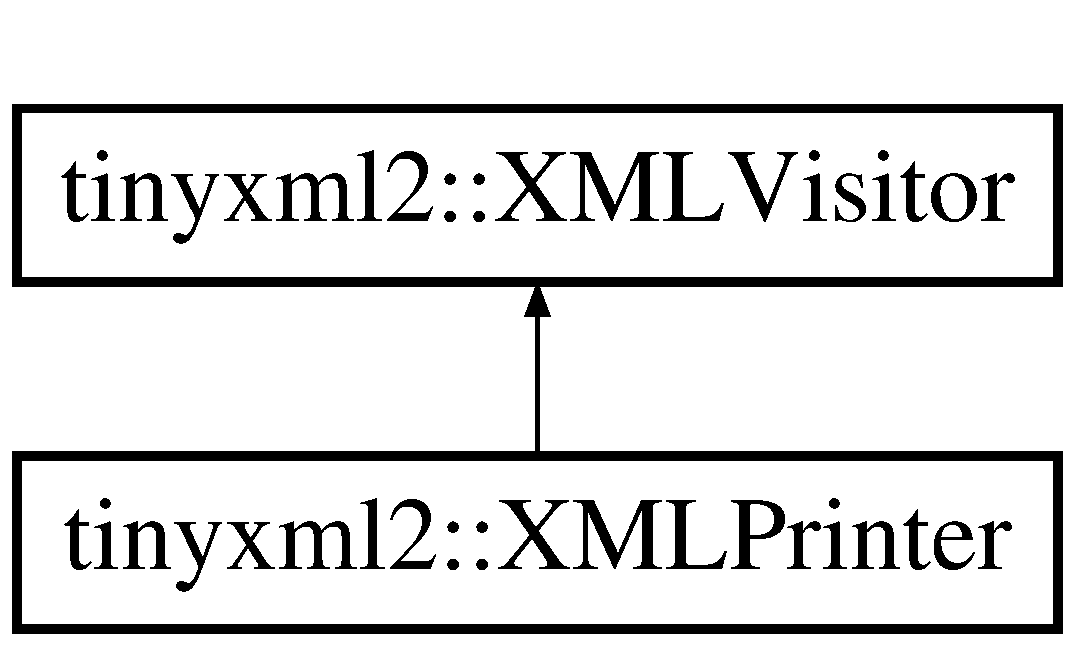
\includegraphics[height=2.000000cm]{classtinyxml2_1_1_x_m_l_visitor}
\end{center}
\end{figure}
\subsection*{Public Member Functions}
\begin{DoxyCompactItemize}
\item 
virtual \hyperlink{classtinyxml2_1_1_x_m_l_visitor_a494e72033d646c47d9c65c502ec62364}{$\sim$\+X\+M\+L\+Visitor} ()
\item 
virtual bool \hyperlink{classtinyxml2_1_1_x_m_l_visitor_acb3c22fc5f60eb9db98f533f2761f67d}{Visit\+Enter} (const \hyperlink{classtinyxml2_1_1_x_m_l_document}{X\+M\+L\+Document} \&)
\begin{DoxyCompactList}\small\item\em Visit a document. \end{DoxyCompactList}\item 
virtual bool \hyperlink{classtinyxml2_1_1_x_m_l_visitor_a170e9989cd046ba904f302d087e07086}{Visit\+Exit} (const \hyperlink{classtinyxml2_1_1_x_m_l_document}{X\+M\+L\+Document} \&)
\begin{DoxyCompactList}\small\item\em Visit a document. \end{DoxyCompactList}\item 
virtual bool \hyperlink{classtinyxml2_1_1_x_m_l_visitor_af97980a17dd4e37448b181f5ddfa92b5}{Visit\+Enter} (const \hyperlink{classtinyxml2_1_1_x_m_l_element}{X\+M\+L\+Element} \&, const \hyperlink{classtinyxml2_1_1_x_m_l_attribute}{X\+M\+L\+Attribute} $\ast$)
\begin{DoxyCompactList}\small\item\em Visit an element. \end{DoxyCompactList}\item 
virtual bool \hyperlink{classtinyxml2_1_1_x_m_l_visitor_a772f10ddc83f881956d32628faa16eb6}{Visit\+Exit} (const \hyperlink{classtinyxml2_1_1_x_m_l_element}{X\+M\+L\+Element} \&)
\begin{DoxyCompactList}\small\item\em Visit an element. \end{DoxyCompactList}\item 
virtual bool \hyperlink{classtinyxml2_1_1_x_m_l_visitor_adc75bd459fc7ba8223b50f0616767f9a}{Visit} (const \hyperlink{classtinyxml2_1_1_x_m_l_declaration}{X\+M\+L\+Declaration} \&)
\begin{DoxyCompactList}\small\item\em Visit a declaration. \end{DoxyCompactList}\item 
virtual bool \hyperlink{classtinyxml2_1_1_x_m_l_visitor_af30233565856480ea48b6fa0d6dec65b}{Visit} (const \hyperlink{classtinyxml2_1_1_x_m_l_text}{X\+M\+L\+Text} \&)
\begin{DoxyCompactList}\small\item\em Visit a text node. \end{DoxyCompactList}\item 
virtual bool \hyperlink{classtinyxml2_1_1_x_m_l_visitor_acc8147fb5a85f6c65721654e427752d7}{Visit} (const \hyperlink{classtinyxml2_1_1_x_m_l_comment}{X\+M\+L\+Comment} \&)
\begin{DoxyCompactList}\small\item\em Visit a comment node. \end{DoxyCompactList}\item 
virtual bool \hyperlink{classtinyxml2_1_1_x_m_l_visitor_a14e4748387c34bf53d24e8119bb1f292}{Visit} (const \hyperlink{classtinyxml2_1_1_x_m_l_unknown}{X\+M\+L\+Unknown} \&)
\begin{DoxyCompactList}\small\item\em Visit an unknown node. \end{DoxyCompactList}\end{DoxyCompactItemize}


\subsection{Detailed Description}
Implements the interface to the \char`\"{}\+Visitor pattern\char`\"{} (see the Accept() method.) If you call the Accept() method, it requires being passed a \hyperlink{classtinyxml2_1_1_x_m_l_visitor}{X\+M\+L\+Visitor} class to handle callbacks. For nodes that contain other nodes (Document, Element) you will get called with a Visit\+Enter/\+Visit\+Exit pair. Nodes that are always leafs are simply called with \hyperlink{classtinyxml2_1_1_x_m_l_visitor_adc75bd459fc7ba8223b50f0616767f9a}{Visit()}.

If you return \textquotesingle{}true\textquotesingle{} from a Visit method, recursive parsing will continue. If you return false, {\bfseries no children of this node or its siblings} will be visited.

All flavors of Visit methods have a default implementation that returns \textquotesingle{}true\textquotesingle{} (continue visiting). You need to only override methods that are interesting to you.

Generally Accept() is called on the \hyperlink{classtinyxml2_1_1_x_m_l_document}{X\+M\+L\+Document}, although all nodes support visiting.

You should never change the document from a callback.

\begin{DoxySeeAlso}{See also}
\hyperlink{classtinyxml2_1_1_x_m_l_node_a81e66df0a44c67a7af17f3b77a152785}{X\+M\+L\+Node\+::\+Accept()} 
\end{DoxySeeAlso}


\subsection{Constructor \& Destructor Documentation}
\hypertarget{classtinyxml2_1_1_x_m_l_visitor_a494e72033d646c47d9c65c502ec62364}{}\index{tinyxml2\+::\+X\+M\+L\+Visitor@{tinyxml2\+::\+X\+M\+L\+Visitor}!````~X\+M\+L\+Visitor@{$\sim$\+X\+M\+L\+Visitor}}
\index{````~X\+M\+L\+Visitor@{$\sim$\+X\+M\+L\+Visitor}!tinyxml2\+::\+X\+M\+L\+Visitor@{tinyxml2\+::\+X\+M\+L\+Visitor}}
\subsubsection[{$\sim$\+X\+M\+L\+Visitor}]{\setlength{\rightskip}{0pt plus 5cm}virtual tinyxml2\+::\+X\+M\+L\+Visitor\+::$\sim$\+X\+M\+L\+Visitor (
\begin{DoxyParamCaption}
{}
\end{DoxyParamCaption}
)\hspace{0.3cm}{\ttfamily [inline]}, {\ttfamily [virtual]}}\label{classtinyxml2_1_1_x_m_l_visitor_a494e72033d646c47d9c65c502ec62364}


\subsection{Member Function Documentation}
\hypertarget{classtinyxml2_1_1_x_m_l_visitor_adc75bd459fc7ba8223b50f0616767f9a}{}\index{tinyxml2\+::\+X\+M\+L\+Visitor@{tinyxml2\+::\+X\+M\+L\+Visitor}!Visit@{Visit}}
\index{Visit@{Visit}!tinyxml2\+::\+X\+M\+L\+Visitor@{tinyxml2\+::\+X\+M\+L\+Visitor}}
\subsubsection[{Visit}]{\setlength{\rightskip}{0pt plus 5cm}virtual bool tinyxml2\+::\+X\+M\+L\+Visitor\+::\+Visit (
\begin{DoxyParamCaption}
\item[{const {\bf X\+M\+L\+Declaration} \&}]{}
\end{DoxyParamCaption}
)\hspace{0.3cm}{\ttfamily [inline]}, {\ttfamily [virtual]}}\label{classtinyxml2_1_1_x_m_l_visitor_adc75bd459fc7ba8223b50f0616767f9a}


Visit a declaration. 



Reimplemented in \hyperlink{classtinyxml2_1_1_x_m_l_printer_acfc625b2549304b9c7eb85ebd5c5eb39}{tinyxml2\+::\+X\+M\+L\+Printer}.

\hypertarget{classtinyxml2_1_1_x_m_l_visitor_af30233565856480ea48b6fa0d6dec65b}{}\index{tinyxml2\+::\+X\+M\+L\+Visitor@{tinyxml2\+::\+X\+M\+L\+Visitor}!Visit@{Visit}}
\index{Visit@{Visit}!tinyxml2\+::\+X\+M\+L\+Visitor@{tinyxml2\+::\+X\+M\+L\+Visitor}}
\subsubsection[{Visit}]{\setlength{\rightskip}{0pt plus 5cm}virtual bool tinyxml2\+::\+X\+M\+L\+Visitor\+::\+Visit (
\begin{DoxyParamCaption}
\item[{const {\bf X\+M\+L\+Text} \&}]{}
\end{DoxyParamCaption}
)\hspace{0.3cm}{\ttfamily [inline]}, {\ttfamily [virtual]}}\label{classtinyxml2_1_1_x_m_l_visitor_af30233565856480ea48b6fa0d6dec65b}


Visit a text node. 



Reimplemented in \hyperlink{classtinyxml2_1_1_x_m_l_printer_adc0e42b4f6fcb90a95630c79575d030b}{tinyxml2\+::\+X\+M\+L\+Printer}.

\hypertarget{classtinyxml2_1_1_x_m_l_visitor_acc8147fb5a85f6c65721654e427752d7}{}\index{tinyxml2\+::\+X\+M\+L\+Visitor@{tinyxml2\+::\+X\+M\+L\+Visitor}!Visit@{Visit}}
\index{Visit@{Visit}!tinyxml2\+::\+X\+M\+L\+Visitor@{tinyxml2\+::\+X\+M\+L\+Visitor}}
\subsubsection[{Visit}]{\setlength{\rightskip}{0pt plus 5cm}virtual bool tinyxml2\+::\+X\+M\+L\+Visitor\+::\+Visit (
\begin{DoxyParamCaption}
\item[{const {\bf X\+M\+L\+Comment} \&}]{}
\end{DoxyParamCaption}
)\hspace{0.3cm}{\ttfamily [inline]}, {\ttfamily [virtual]}}\label{classtinyxml2_1_1_x_m_l_visitor_acc8147fb5a85f6c65721654e427752d7}


Visit a comment node. 



Reimplemented in \hyperlink{classtinyxml2_1_1_x_m_l_printer_aa294c5c01af0ebb9114902456e4cb53c}{tinyxml2\+::\+X\+M\+L\+Printer}.

\hypertarget{classtinyxml2_1_1_x_m_l_visitor_a14e4748387c34bf53d24e8119bb1f292}{}\index{tinyxml2\+::\+X\+M\+L\+Visitor@{tinyxml2\+::\+X\+M\+L\+Visitor}!Visit@{Visit}}
\index{Visit@{Visit}!tinyxml2\+::\+X\+M\+L\+Visitor@{tinyxml2\+::\+X\+M\+L\+Visitor}}
\subsubsection[{Visit}]{\setlength{\rightskip}{0pt plus 5cm}virtual bool tinyxml2\+::\+X\+M\+L\+Visitor\+::\+Visit (
\begin{DoxyParamCaption}
\item[{const {\bf X\+M\+L\+Unknown} \&}]{}
\end{DoxyParamCaption}
)\hspace{0.3cm}{\ttfamily [inline]}, {\ttfamily [virtual]}}\label{classtinyxml2_1_1_x_m_l_visitor_a14e4748387c34bf53d24e8119bb1f292}


Visit an unknown node. 



Reimplemented in \hyperlink{classtinyxml2_1_1_x_m_l_printer_ab8af5455bbf9e4be2663e6642fcd7e32}{tinyxml2\+::\+X\+M\+L\+Printer}.

\hypertarget{classtinyxml2_1_1_x_m_l_visitor_acb3c22fc5f60eb9db98f533f2761f67d}{}\index{tinyxml2\+::\+X\+M\+L\+Visitor@{tinyxml2\+::\+X\+M\+L\+Visitor}!Visit\+Enter@{Visit\+Enter}}
\index{Visit\+Enter@{Visit\+Enter}!tinyxml2\+::\+X\+M\+L\+Visitor@{tinyxml2\+::\+X\+M\+L\+Visitor}}
\subsubsection[{Visit\+Enter}]{\setlength{\rightskip}{0pt plus 5cm}virtual bool tinyxml2\+::\+X\+M\+L\+Visitor\+::\+Visit\+Enter (
\begin{DoxyParamCaption}
\item[{const {\bf X\+M\+L\+Document} \&}]{}
\end{DoxyParamCaption}
)\hspace{0.3cm}{\ttfamily [inline]}, {\ttfamily [virtual]}}\label{classtinyxml2_1_1_x_m_l_visitor_acb3c22fc5f60eb9db98f533f2761f67d}


Visit a document. 



Reimplemented in \hyperlink{classtinyxml2_1_1_x_m_l_printer_a9aa1de11a55a07db55a90fde37d7afad}{tinyxml2\+::\+X\+M\+L\+Printer}.

\hypertarget{classtinyxml2_1_1_x_m_l_visitor_af97980a17dd4e37448b181f5ddfa92b5}{}\index{tinyxml2\+::\+X\+M\+L\+Visitor@{tinyxml2\+::\+X\+M\+L\+Visitor}!Visit\+Enter@{Visit\+Enter}}
\index{Visit\+Enter@{Visit\+Enter}!tinyxml2\+::\+X\+M\+L\+Visitor@{tinyxml2\+::\+X\+M\+L\+Visitor}}
\subsubsection[{Visit\+Enter}]{\setlength{\rightskip}{0pt plus 5cm}virtual bool tinyxml2\+::\+X\+M\+L\+Visitor\+::\+Visit\+Enter (
\begin{DoxyParamCaption}
\item[{const {\bf X\+M\+L\+Element} \&}]{, }
\item[{const {\bf X\+M\+L\+Attribute} $\ast$}]{}
\end{DoxyParamCaption}
)\hspace{0.3cm}{\ttfamily [inline]}, {\ttfamily [virtual]}}\label{classtinyxml2_1_1_x_m_l_visitor_af97980a17dd4e37448b181f5ddfa92b5}


Visit an element. 



Reimplemented in \hyperlink{classtinyxml2_1_1_x_m_l_printer_a169b2509d8eabb70811b2bb8cfd1f5d1}{tinyxml2\+::\+X\+M\+L\+Printer}.

\hypertarget{classtinyxml2_1_1_x_m_l_visitor_a170e9989cd046ba904f302d087e07086}{}\index{tinyxml2\+::\+X\+M\+L\+Visitor@{tinyxml2\+::\+X\+M\+L\+Visitor}!Visit\+Exit@{Visit\+Exit}}
\index{Visit\+Exit@{Visit\+Exit}!tinyxml2\+::\+X\+M\+L\+Visitor@{tinyxml2\+::\+X\+M\+L\+Visitor}}
\subsubsection[{Visit\+Exit}]{\setlength{\rightskip}{0pt plus 5cm}virtual bool tinyxml2\+::\+X\+M\+L\+Visitor\+::\+Visit\+Exit (
\begin{DoxyParamCaption}
\item[{const {\bf X\+M\+L\+Document} \&}]{}
\end{DoxyParamCaption}
)\hspace{0.3cm}{\ttfamily [inline]}, {\ttfamily [virtual]}}\label{classtinyxml2_1_1_x_m_l_visitor_a170e9989cd046ba904f302d087e07086}


Visit a document. 



Reimplemented in \hyperlink{classtinyxml2_1_1_x_m_l_printer_a15fc1f2b922f540917dcf52808737b29}{tinyxml2\+::\+X\+M\+L\+Printer}.

\hypertarget{classtinyxml2_1_1_x_m_l_visitor_a772f10ddc83f881956d32628faa16eb6}{}\index{tinyxml2\+::\+X\+M\+L\+Visitor@{tinyxml2\+::\+X\+M\+L\+Visitor}!Visit\+Exit@{Visit\+Exit}}
\index{Visit\+Exit@{Visit\+Exit}!tinyxml2\+::\+X\+M\+L\+Visitor@{tinyxml2\+::\+X\+M\+L\+Visitor}}
\subsubsection[{Visit\+Exit}]{\setlength{\rightskip}{0pt plus 5cm}virtual bool tinyxml2\+::\+X\+M\+L\+Visitor\+::\+Visit\+Exit (
\begin{DoxyParamCaption}
\item[{const {\bf X\+M\+L\+Element} \&}]{}
\end{DoxyParamCaption}
)\hspace{0.3cm}{\ttfamily [inline]}, {\ttfamily [virtual]}}\label{classtinyxml2_1_1_x_m_l_visitor_a772f10ddc83f881956d32628faa16eb6}


Visit an element. 



Reimplemented in \hyperlink{classtinyxml2_1_1_x_m_l_printer_a2edd48405971a88951c71c9df86a2f50}{tinyxml2\+::\+X\+M\+L\+Printer}.



The documentation for this class was generated from the following file\+:\begin{DoxyCompactItemize}
\item 
\hyperlink{tinyxml2_8h}{tinyxml2.\+h}\end{DoxyCompactItemize}

\chapter{File Documentation}
\hypertarget{_animator_8cpp}{}\section{Animator.\+cpp File Reference}
\label{_animator_8cpp}\index{Animator.\+cpp@{Animator.\+cpp}}
{\ttfamily \#include \char`\"{}Animator.\+h\char`\"{}}\\*

\hypertarget{_animator_8h}{}\section{Animator.\+h File Reference}
\label{_animator_8h}\index{Animator.\+h@{Animator.\+h}}
{\ttfamily \#include $<$T\+I\+N\+Y\+X\+M\+L2\textbackslash{}tinyxml2.\+h$>$}\\*
{\ttfamily \#include \char`\"{}Sprite.\+h\char`\"{}}\\*
\subsection*{Classes}
\begin{DoxyCompactItemize}
\item 
struct \hyperlink{struct_sprite_data}{Sprite\+Data}
\begin{DoxyCompactList}\small\item\em holds sprite U\+V data \end{DoxyCompactList}\item 
struct \hyperlink{struct_atlas}{Atlas}
\begin{DoxyCompactList}\small\item\em holds atlas data \end{DoxyCompactList}\item 
class \hyperlink{class_animator}{Animator}
\begin{DoxyCompactList}\small\item\em stores atlas texture and changes sprite U\+V accordingly to perform animation \end{DoxyCompactList}\end{DoxyCompactItemize}
\subsection*{Variables}
\begin{DoxyCompactItemize}
\item 
const int \hyperlink{_animator_8h_a2e880c677ee810c3f221b3b5636ff7e0}{M\+A\+X\+S\+P\+R\+I\+T\+E} = 30
\begin{DoxyCompactList}\small\item\em This file takes in multiple sprites and outputs them as an animation //. \end{DoxyCompactList}\end{DoxyCompactItemize}


\subsection{Variable Documentation}
\hypertarget{_animator_8h_a2e880c677ee810c3f221b3b5636ff7e0}{}\index{Animator.\+h@{Animator.\+h}!M\+A\+X\+S\+P\+R\+I\+T\+E@{M\+A\+X\+S\+P\+R\+I\+T\+E}}
\index{M\+A\+X\+S\+P\+R\+I\+T\+E@{M\+A\+X\+S\+P\+R\+I\+T\+E}!Animator.\+h@{Animator.\+h}}
\subsubsection[{M\+A\+X\+S\+P\+R\+I\+T\+E}]{\setlength{\rightskip}{0pt plus 5cm}const int M\+A\+X\+S\+P\+R\+I\+T\+E = 30}\label{_animator_8h_a2e880c677ee810c3f221b3b5636ff7e0}


This file takes in multiple sprites and outputs them as an animation //. 

sets global for max amount of sprites in an animation 
\hypertarget{main_8cpp}{}\section{main.\+cpp File Reference}
\label{main_8cpp}\index{main.\+cpp@{main.\+cpp}}
{\ttfamily \#include \char`\"{}quad.\+h\char`\"{}}\\*
{\ttfamily \#include \char`\"{}Sprite.\+h\char`\"{}}\\*
{\ttfamily \#include \char`\"{}Text.\+h\char`\"{}}\\*
{\ttfamily \#include \char`\"{}Animator.\+h\char`\"{}}\\*
\subsection*{Functions}
\begin{DoxyCompactItemize}
\item 
int \hyperlink{main_8cpp_ae66f6b31b5ad750f1fe042a706a4e3d4}{main} ()
\end{DoxyCompactItemize}


\subsection{Function Documentation}
\hypertarget{main_8cpp_ae66f6b31b5ad750f1fe042a706a4e3d4}{}\index{main.\+cpp@{main.\+cpp}!main@{main}}
\index{main@{main}!main.\+cpp@{main.\+cpp}}
\subsubsection[{main}]{\setlength{\rightskip}{0pt plus 5cm}int main (
\begin{DoxyParamCaption}
{}
\end{DoxyParamCaption}
)}\label{main_8cpp_ae66f6b31b5ad750f1fe042a706a4e3d4}

\hypertarget{quad_8cpp}{}\section{quad.\+cpp File Reference}
\label{quad_8cpp}\index{quad.\+cpp@{quad.\+cpp}}
{\ttfamily \#include \char`\"{}quad.\+h\char`\"{}}\\*
\subsection*{Functions}
\begin{DoxyCompactItemize}
\item 
void \hyperlink{quad_8cpp_a4fa209694361959d09cd504f86d2466f}{Initialize} (const char $\ast$window\+Title, int window\+Width, int window\+Height)
\begin{DoxyCompactList}\small\item\em initilizes and creates glfw window with error checking \end{DoxyCompactList}\item 
bool \hyperlink{quad_8cpp_a130105f5407c84602eea0f49c05ca397}{Framework\+Update} ()
\begin{DoxyCompactList}\small\item\em returns if the window should close \end{DoxyCompactList}\item 
void \hyperlink{quad_8cpp_adbf0ac289c6c48a75de9d75dc34e9ace}{Orthographic} (float a\+\_\+f\+Left, float a\+\_\+f\+Right, float a\+\_\+f\+Top, float a\+\_\+f\+Bottom, float a\+\_\+f\+Near, float a\+\_\+f\+Far, \hyperlink{_sprite_8h_a2db59f395fe82a7394c6324956c265d8}{glm\+::mat4} \&mat)
\begin{DoxyCompactList}\small\item\em changes data of vertex points to an orthographic projection \end{DoxyCompactList}\end{DoxyCompactItemize}
\subsection*{Variables}
\begin{DoxyCompactItemize}
\item 
int \hyperlink{quad_8cpp_a2474a5474cbff19523a51eb1de01cda4}{width}
\begin{DoxyCompactList}\small\item\em gloabal variables for widndow width and height \end{DoxyCompactList}\item 
int \hyperlink{quad_8cpp_ad12fc34ce789bce6c8a05d8a17138534}{height}
\item 
G\+L\+F\+Wwindow $\ast$ \hyperlink{quad_8cpp_a80de27bd7dc4e2b2ad3d5895b97a70f0}{window}
\begin{DoxyCompactList}\small\item\em global variable for G\+L\+F\+W window \end{DoxyCompactList}\item 
\hyperlink{_sprite_8h_a2db59f395fe82a7394c6324956c265d8}{glm\+::mat4} \hyperlink{quad_8cpp_ad89bd72040d0dfc083b4176db9b3a631}{Ortho}
\begin{DoxyCompactList}\small\item\em global matrix of a matrix of size 4x4 for orhtographic projection calculation \end{DoxyCompactList}\end{DoxyCompactItemize}


\subsection{Function Documentation}
\hypertarget{quad_8cpp_a130105f5407c84602eea0f49c05ca397}{}\index{quad.\+cpp@{quad.\+cpp}!Framework\+Update@{Framework\+Update}}
\index{Framework\+Update@{Framework\+Update}!quad.\+cpp@{quad.\+cpp}}
\subsubsection[{Framework\+Update}]{\setlength{\rightskip}{0pt plus 5cm}bool Framework\+Update (
\begin{DoxyParamCaption}
{}
\end{DoxyParamCaption}
)}\label{quad_8cpp_a130105f5407c84602eea0f49c05ca397}


returns if the window should close 

\hypertarget{quad_8cpp_a4fa209694361959d09cd504f86d2466f}{}\index{quad.\+cpp@{quad.\+cpp}!Initialize@{Initialize}}
\index{Initialize@{Initialize}!quad.\+cpp@{quad.\+cpp}}
\subsubsection[{Initialize}]{\setlength{\rightskip}{0pt plus 5cm}void Initialize (
\begin{DoxyParamCaption}
\item[{const char $\ast$}]{window\+Title, }
\item[{int}]{window\+Width, }
\item[{int}]{window\+Height}
\end{DoxyParamCaption}
)}\label{quad_8cpp_a4fa209694361959d09cd504f86d2466f}


initilizes and creates glfw window with error checking 


\begin{DoxyParams}{Parameters}
{\em takes} & in the name of window \\
\hline
{\em window} & width \\
\hline
{\em window} & height \\
\hline
\end{DoxyParams}
\hypertarget{quad_8cpp_adbf0ac289c6c48a75de9d75dc34e9ace}{}\index{quad.\+cpp@{quad.\+cpp}!Orthographic@{Orthographic}}
\index{Orthographic@{Orthographic}!quad.\+cpp@{quad.\+cpp}}
\subsubsection[{Orthographic}]{\setlength{\rightskip}{0pt plus 5cm}void Orthographic (
\begin{DoxyParamCaption}
\item[{float}]{a\+\_\+f\+Left, }
\item[{float}]{a\+\_\+f\+Right, }
\item[{float}]{a\+\_\+f\+Top, }
\item[{float}]{a\+\_\+f\+Bottom, }
\item[{float}]{a\+\_\+f\+Near, }
\item[{float}]{a\+\_\+f\+Far, }
\item[{{\bf glm\+::mat4} \&}]{mat}
\end{DoxyParamCaption}
)}\label{quad_8cpp_adbf0ac289c6c48a75de9d75dc34e9ace}


changes data of vertex points to an orthographic projection 


\begin{DoxyParams}{Parameters}
{\em takes} & left, right, top, bottom, near, and far position and saves to mat \\
\hline
\end{DoxyParams}


\subsection{Variable Documentation}
\hypertarget{quad_8cpp_ad12fc34ce789bce6c8a05d8a17138534}{}\index{quad.\+cpp@{quad.\+cpp}!height@{height}}
\index{height@{height}!quad.\+cpp@{quad.\+cpp}}
\subsubsection[{height}]{\setlength{\rightskip}{0pt plus 5cm}int height}\label{quad_8cpp_ad12fc34ce789bce6c8a05d8a17138534}
\hypertarget{quad_8cpp_ad89bd72040d0dfc083b4176db9b3a631}{}\index{quad.\+cpp@{quad.\+cpp}!Ortho@{Ortho}}
\index{Ortho@{Ortho}!quad.\+cpp@{quad.\+cpp}}
\subsubsection[{Ortho}]{\setlength{\rightskip}{0pt plus 5cm}{\bf glm\+::mat4} Ortho}\label{quad_8cpp_ad89bd72040d0dfc083b4176db9b3a631}


global matrix of a matrix of size 4x4 for orhtographic projection calculation 

\hypertarget{quad_8cpp_a2474a5474cbff19523a51eb1de01cda4}{}\index{quad.\+cpp@{quad.\+cpp}!width@{width}}
\index{width@{width}!quad.\+cpp@{quad.\+cpp}}
\subsubsection[{width}]{\setlength{\rightskip}{0pt plus 5cm}int width}\label{quad_8cpp_a2474a5474cbff19523a51eb1de01cda4}


gloabal variables for widndow width and height 

\hypertarget{quad_8cpp_a80de27bd7dc4e2b2ad3d5895b97a70f0}{}\index{quad.\+cpp@{quad.\+cpp}!window@{window}}
\index{window@{window}!quad.\+cpp@{quad.\+cpp}}
\subsubsection[{window}]{\setlength{\rightskip}{0pt plus 5cm}G\+L\+F\+Wwindow$\ast$ window}\label{quad_8cpp_a80de27bd7dc4e2b2ad3d5895b97a70f0}


global variable for G\+L\+F\+W window 


\hypertarget{quad_8h}{}\section{quad.\+h File Reference}
\label{quad_8h}\index{quad.\+h@{quad.\+h}}
{\ttfamily \#include $<$G\+L\textbackslash{}glew.\+h$>$}\\*
{\ttfamily \#include $<$G\+L\textbackslash{}wglew.\+h$>$}\\*
{\ttfamily \#include $<$G\+L\+F\+W\textbackslash{}glfw3.\+h$>$}\\*
{\ttfamily \#include $<$S\+O\+I\+L\textbackslash{}\+S\+O\+I\+L.\+h$>$}\\*
{\ttfamily \#include $<$glm\textbackslash{}glm.\+hpp$>$}\\*
{\ttfamily \#include $<$glm\textbackslash{}gtc\textbackslash{}matrix\+\_\+transform.\+hpp$>$}\\*
{\ttfamily \#include $<$glm\textbackslash{}gtc\textbackslash{}type\+\_\+ptr.\+hpp$>$}\\*
{\ttfamily \#include $<$iostream$>$}\\*
{\ttfamily \#include $<$vector$>$}\\*
{\ttfamily \#include $<$string$>$}\\*
{\ttfamily \#include $<$fstream$>$}\\*
\subsection*{Classes}
\begin{DoxyCompactItemize}
\item 
struct \hyperlink{struct_vertex}{Vertex}
\begin{DoxyCompactList}\small\item\em holds data for each vertex of the quad \end{DoxyCompactList}\item 
class \hyperlink{class_quad}{Quad}
\begin{DoxyCompactList}\small\item\em creates verticies and shaders for quad and stores them in the V\+B\+O \end{DoxyCompactList}\end{DoxyCompactItemize}
\subsection*{Functions}
\begin{DoxyCompactItemize}
\item 
void \hyperlink{quad_8h_a4fa209694361959d09cd504f86d2466f}{Initialize} (const char $\ast$window\+Title, int window\+Width, int window\+Height)
\begin{DoxyCompactList}\small\item\em initilizes and creates glfw window with error checking \end{DoxyCompactList}\item 
bool \hyperlink{quad_8h_a130105f5407c84602eea0f49c05ca397}{Framework\+Update} ()
\begin{DoxyCompactList}\small\item\em returns if the window should close \end{DoxyCompactList}\item 
void \hyperlink{quad_8h_adbf0ac289c6c48a75de9d75dc34e9ace}{Orthographic} (float a\+\_\+f\+Left, float a\+\_\+f\+Right, float a\+\_\+f\+Top, float a\+\_\+f\+Bottom, float a\+\_\+f\+Near, float a\+\_\+f\+Far, \hyperlink{_sprite_8h_a2db59f395fe82a7394c6324956c265d8}{glm\+::mat4} \&mat)
\begin{DoxyCompactList}\small\item\em changes data of vertex points to an orthographic projection \end{DoxyCompactList}\end{DoxyCompactItemize}
\subsection*{Variables}
\begin{DoxyCompactItemize}
\item 
const int \hyperlink{quad_8h_a8b8c1399b3ff5d8fdc5b7352549ef604}{M\+A\+X\+S\+P\+R\+I\+T\+E\+S} = 30
\begin{DoxyCompactList}\small\item\em initialize maximum amount of sprites \end{DoxyCompactList}\item 
int \hyperlink{quad_8h_a2474a5474cbff19523a51eb1de01cda4}{width}
\begin{DoxyCompactList}\small\item\em gloabal variables for widndow width and height \end{DoxyCompactList}\item 
int \hyperlink{quad_8h_ad12fc34ce789bce6c8a05d8a17138534}{height}
\item 
G\+L\+F\+Wwindow $\ast$ \hyperlink{quad_8h_a80de27bd7dc4e2b2ad3d5895b97a70f0}{window}
\begin{DoxyCompactList}\small\item\em global variable for G\+L\+F\+W window \end{DoxyCompactList}\item 
\hyperlink{_sprite_8h_a2db59f395fe82a7394c6324956c265d8}{glm\+::mat4} \hyperlink{quad_8h_ad89bd72040d0dfc083b4176db9b3a631}{Ortho}
\begin{DoxyCompactList}\small\item\em global matrix of a matrix of size 4x4 for orhtographic projection calculation \end{DoxyCompactList}\end{DoxyCompactItemize}


\subsection{Function Documentation}
\hypertarget{quad_8h_a130105f5407c84602eea0f49c05ca397}{}\index{quad.\+h@{quad.\+h}!Framework\+Update@{Framework\+Update}}
\index{Framework\+Update@{Framework\+Update}!quad.\+h@{quad.\+h}}
\subsubsection[{Framework\+Update}]{\setlength{\rightskip}{0pt plus 5cm}bool Framework\+Update (
\begin{DoxyParamCaption}
{}
\end{DoxyParamCaption}
)}\label{quad_8h_a130105f5407c84602eea0f49c05ca397}


returns if the window should close 

\hypertarget{quad_8h_a4fa209694361959d09cd504f86d2466f}{}\index{quad.\+h@{quad.\+h}!Initialize@{Initialize}}
\index{Initialize@{Initialize}!quad.\+h@{quad.\+h}}
\subsubsection[{Initialize}]{\setlength{\rightskip}{0pt plus 5cm}void Initialize (
\begin{DoxyParamCaption}
\item[{const char $\ast$}]{window\+Title, }
\item[{int}]{window\+Width, }
\item[{int}]{window\+Height}
\end{DoxyParamCaption}
)}\label{quad_8h_a4fa209694361959d09cd504f86d2466f}


initilizes and creates glfw window with error checking 


\begin{DoxyParams}{Parameters}
{\em takes} & in the name of window \\
\hline
{\em window} & width \\
\hline
{\em window} & height \\
\hline
\end{DoxyParams}
\hypertarget{quad_8h_adbf0ac289c6c48a75de9d75dc34e9ace}{}\index{quad.\+h@{quad.\+h}!Orthographic@{Orthographic}}
\index{Orthographic@{Orthographic}!quad.\+h@{quad.\+h}}
\subsubsection[{Orthographic}]{\setlength{\rightskip}{0pt plus 5cm}void Orthographic (
\begin{DoxyParamCaption}
\item[{float}]{a\+\_\+f\+Left, }
\item[{float}]{a\+\_\+f\+Right, }
\item[{float}]{a\+\_\+f\+Top, }
\item[{float}]{a\+\_\+f\+Bottom, }
\item[{float}]{a\+\_\+f\+Near, }
\item[{float}]{a\+\_\+f\+Far, }
\item[{{\bf glm\+::mat4} \&}]{mat}
\end{DoxyParamCaption}
)}\label{quad_8h_adbf0ac289c6c48a75de9d75dc34e9ace}


changes data of vertex points to an orthographic projection 


\begin{DoxyParams}{Parameters}
{\em takes} & left, right, top, bottom, near, and far position and saves to mat \\
\hline
\end{DoxyParams}


\subsection{Variable Documentation}
\hypertarget{quad_8h_ad12fc34ce789bce6c8a05d8a17138534}{}\index{quad.\+h@{quad.\+h}!height@{height}}
\index{height@{height}!quad.\+h@{quad.\+h}}
\subsubsection[{height}]{\setlength{\rightskip}{0pt plus 5cm}int height}\label{quad_8h_ad12fc34ce789bce6c8a05d8a17138534}
\hypertarget{quad_8h_a8b8c1399b3ff5d8fdc5b7352549ef604}{}\index{quad.\+h@{quad.\+h}!M\+A\+X\+S\+P\+R\+I\+T\+E\+S@{M\+A\+X\+S\+P\+R\+I\+T\+E\+S}}
\index{M\+A\+X\+S\+P\+R\+I\+T\+E\+S@{M\+A\+X\+S\+P\+R\+I\+T\+E\+S}!quad.\+h@{quad.\+h}}
\subsubsection[{M\+A\+X\+S\+P\+R\+I\+T\+E\+S}]{\setlength{\rightskip}{0pt plus 5cm}const int M\+A\+X\+S\+P\+R\+I\+T\+E\+S = 30}\label{quad_8h_a8b8c1399b3ff5d8fdc5b7352549ef604}


initialize maximum amount of sprites 

This file creates quad, allocate memory on the buffer for it, and saves the data. // The quad data includes shader data, vertex transforms from orthographic projection // \hyperlink{class_quad}{Quad} also initializes the Open\+G\+L window. // \hypertarget{quad_8h_ad89bd72040d0dfc083b4176db9b3a631}{}\index{quad.\+h@{quad.\+h}!Ortho@{Ortho}}
\index{Ortho@{Ortho}!quad.\+h@{quad.\+h}}
\subsubsection[{Ortho}]{\setlength{\rightskip}{0pt plus 5cm}{\bf glm\+::mat4} Ortho}\label{quad_8h_ad89bd72040d0dfc083b4176db9b3a631}


global matrix of a matrix of size 4x4 for orhtographic projection calculation 

\hypertarget{quad_8h_a2474a5474cbff19523a51eb1de01cda4}{}\index{quad.\+h@{quad.\+h}!width@{width}}
\index{width@{width}!quad.\+h@{quad.\+h}}
\subsubsection[{width}]{\setlength{\rightskip}{0pt plus 5cm}int width}\label{quad_8h_a2474a5474cbff19523a51eb1de01cda4}


gloabal variables for widndow width and height 

\hypertarget{quad_8h_a80de27bd7dc4e2b2ad3d5895b97a70f0}{}\index{quad.\+h@{quad.\+h}!window@{window}}
\index{window@{window}!quad.\+h@{quad.\+h}}
\subsubsection[{window}]{\setlength{\rightskip}{0pt plus 5cm}G\+L\+F\+Wwindow$\ast$ window}\label{quad_8h_a80de27bd7dc4e2b2ad3d5895b97a70f0}


global variable for G\+L\+F\+W window 


\hypertarget{_sprite_8cpp}{}\section{Sprite.\+cpp File Reference}
\label{_sprite_8cpp}\index{Sprite.\+cpp@{Sprite.\+cpp}}
{\ttfamily \#include \char`\"{}Sprite.\+h\char`\"{}}\\*

\hypertarget{_sprite_8h}{}\section{Sprite.\+h File Reference}
\label{_sprite_8h}\index{Sprite.\+h@{Sprite.\+h}}
{\ttfamily \#include \char`\"{}quad.\+h\char`\"{}}\\*
{\ttfamily \#include $<$glm\textbackslash{}glm.\+hpp$>$}\\*
{\ttfamily \#include $<$glm\textbackslash{}gtc\textbackslash{}matrix\+\_\+transform.\+hpp$>$}\\*
\subsection*{Classes}
\begin{DoxyCompactItemize}
\item 
class \hyperlink{class_sprite}{Sprite}
\begin{DoxyCompactList}\small\item\em reads and creates texture for a quad \end{DoxyCompactList}\end{DoxyCompactItemize}
\subsection*{Typedefs}
\begin{DoxyCompactItemize}
\item 
typedef glm\+::mat4 \hyperlink{_sprite_8h_a2db59f395fe82a7394c6324956c265d8}{mat4}
\begin{DoxyCompactList}\small\item\em type defining glm mat4 for ease of use \end{DoxyCompactList}\item 
typedef glm\+::vec3 \hyperlink{_sprite_8h_a3d0ce73e3199de81565fb01632415288}{vec3}
\begin{DoxyCompactList}\small\item\em type defining glm vec3 for ease of use \end{DoxyCompactList}\end{DoxyCompactItemize}


\subsection{Typedef Documentation}
\hypertarget{_sprite_8h_a2db59f395fe82a7394c6324956c265d8}{}\index{Sprite.\+h@{Sprite.\+h}!mat4@{mat4}}
\index{mat4@{mat4}!Sprite.\+h@{Sprite.\+h}}
\subsubsection[{mat4}]{\setlength{\rightskip}{0pt plus 5cm}typedef glm\+::mat4 {\bf mat4}}\label{_sprite_8h_a2db59f395fe82a7394c6324956c265d8}


type defining glm mat4 for ease of use 

\hypertarget{_sprite_8h_a3d0ce73e3199de81565fb01632415288}{}\index{Sprite.\+h@{Sprite.\+h}!vec3@{vec3}}
\index{vec3@{vec3}!Sprite.\+h@{Sprite.\+h}}
\subsubsection[{vec3}]{\setlength{\rightskip}{0pt plus 5cm}typedef glm\+::vec3 {\bf vec3}}\label{_sprite_8h_a3d0ce73e3199de81565fb01632415288}


type defining glm vec3 for ease of use 


\hypertarget{_text_8cpp}{}\section{Text.\+cpp File Reference}
\label{_text_8cpp}\index{Text.\+cpp@{Text.\+cpp}}
{\ttfamily \#include \char`\"{}Text.\+h\char`\"{}}\\*

\hypertarget{_text_8h}{}\section{Text.\+h File Reference}
\label{_text_8h}\index{Text.\+h@{Text.\+h}}
{\ttfamily \#include $<$T\+I\+N\+Y\+X\+M\+L2\textbackslash{}tinyxml2.\+h$>$}\\*
{\ttfamily \#include \char`\"{}quad.\+h\char`\"{}}\\*
{\ttfamily \#include \char`\"{}Sprite.\+h\char`\"{}}\\*
{\ttfamily \#include $<$iostream$>$}\\*
{\ttfamily \#include $<$string$>$}\\*
{\ttfamily \#include $<$map$>$}\\*
\subsection*{Classes}
\begin{DoxyCompactItemize}
\item 
struct \hyperlink{struct_text_sheet}{Text\+Sheet}
\begin{DoxyCompactList}\small\item\em stores each letter\textquotesingle{}s data \end{DoxyCompactList}\item 
class \hyperlink{class_text_font}{Text\+Font}
\begin{DoxyCompactList}\small\item\em loads and stores an atlas of letters to draw a string \end{DoxyCompactList}\end{DoxyCompactItemize}

\hypertarget{tinyxml2_8cpp}{}\section{tinyxml2.\+cpp File Reference}
\label{tinyxml2_8cpp}\index{tinyxml2.\+cpp@{tinyxml2.\+cpp}}
{\ttfamily \#include \char`\"{}tinyxml2.\+h\char`\"{}}\\*
{\ttfamily \#include $<$new$>$}\\*
{\ttfamily \#include $<$cstddef$>$}\\*
\subsection*{Classes}
\begin{DoxyCompactItemize}
\item 
struct \hyperlink{structtinyxml2_1_1_entity}{tinyxml2\+::\+Entity}
\end{DoxyCompactItemize}
\subsection*{Namespaces}
\begin{DoxyCompactItemize}
\item 
 \hyperlink{namespacetinyxml2}{tinyxml2}
\end{DoxyCompactItemize}

\hypertarget{tinyxml2_8h}{}\section{tinyxml2.\+h File Reference}
\label{tinyxml2_8h}\index{tinyxml2.\+h@{tinyxml2.\+h}}
{\ttfamily \#include $<$cctype$>$}\\*
{\ttfamily \#include $<$climits$>$}\\*
{\ttfamily \#include $<$cstdio$>$}\\*
{\ttfamily \#include $<$cstdlib$>$}\\*
{\ttfamily \#include $<$cstring$>$}\\*
{\ttfamily \#include $<$cstdarg$>$}\\*
\subsection*{Classes}
\begin{DoxyCompactItemize}
\item 
class \hyperlink{classtinyxml2_1_1_str_pair}{tinyxml2\+::\+Str\+Pair}
\item 
class \hyperlink{classtinyxml2_1_1_dyn_array}{tinyxml2\+::\+Dyn\+Array$<$ T, I\+N\+I\+T $>$}
\item 
class \hyperlink{classtinyxml2_1_1_mem_pool}{tinyxml2\+::\+Mem\+Pool}
\item 
class \hyperlink{classtinyxml2_1_1_mem_pool_t}{tinyxml2\+::\+Mem\+Pool\+T$<$ S\+I\+Z\+E $>$}
\item 
class \hyperlink{classtinyxml2_1_1_x_m_l_visitor}{tinyxml2\+::\+X\+M\+L\+Visitor}
\item 
class \hyperlink{classtinyxml2_1_1_x_m_l_util}{tinyxml2\+::\+X\+M\+L\+Util}
\item 
class \hyperlink{classtinyxml2_1_1_x_m_l_node}{tinyxml2\+::\+X\+M\+L\+Node}
\item 
class \hyperlink{classtinyxml2_1_1_x_m_l_text}{tinyxml2\+::\+X\+M\+L\+Text}
\item 
class \hyperlink{classtinyxml2_1_1_x_m_l_comment}{tinyxml2\+::\+X\+M\+L\+Comment}
\item 
class \hyperlink{classtinyxml2_1_1_x_m_l_declaration}{tinyxml2\+::\+X\+M\+L\+Declaration}
\item 
class \hyperlink{classtinyxml2_1_1_x_m_l_unknown}{tinyxml2\+::\+X\+M\+L\+Unknown}
\item 
class \hyperlink{classtinyxml2_1_1_x_m_l_attribute}{tinyxml2\+::\+X\+M\+L\+Attribute}
\item 
class \hyperlink{classtinyxml2_1_1_x_m_l_element}{tinyxml2\+::\+X\+M\+L\+Element}
\item 
class \hyperlink{classtinyxml2_1_1_x_m_l_document}{tinyxml2\+::\+X\+M\+L\+Document}
\item 
class \hyperlink{classtinyxml2_1_1_x_m_l_handle}{tinyxml2\+::\+X\+M\+L\+Handle}
\item 
class \hyperlink{classtinyxml2_1_1_x_m_l_const_handle}{tinyxml2\+::\+X\+M\+L\+Const\+Handle}
\item 
class \hyperlink{classtinyxml2_1_1_x_m_l_printer}{tinyxml2\+::\+X\+M\+L\+Printer}
\end{DoxyCompactItemize}
\subsection*{Namespaces}
\begin{DoxyCompactItemize}
\item 
 \hyperlink{namespacetinyxml2}{tinyxml2}
\end{DoxyCompactItemize}
\subsection*{Macros}
\begin{DoxyCompactItemize}
\item 
\#define \hyperlink{tinyxml2_8h_a8953517b8490d756ad0bfef40fe5811f}{T\+I\+N\+Y\+X\+M\+L2\+\_\+\+L\+I\+B}
\item 
\#define \hyperlink{tinyxml2_8h_a029877acb3c6fd71698561044953bd14}{T\+I\+X\+M\+L\+A\+S\+S\+E\+R\+T}(x)~\{\}
\item 
\#define \hyperlink{tinyxml2_8h_afc6433f9b56e4f18833089b1df629e0a}{T\+I\+X\+M\+L\+\_\+\+S\+N\+P\+R\+I\+N\+T\+F}~snprintf
\item 
\#define \hyperlink{tinyxml2_8h_a96f54d7c855ad92e705510904a040393}{T\+I\+X\+M\+L\+\_\+\+S\+S\+C\+A\+N\+F}~sscanf
\end{DoxyCompactItemize}
\subsection*{Enumerations}
\begin{DoxyCompactItemize}
\item 
enum \hyperlink{namespacetinyxml2_a1fbf88509c3ac88c09117b1947414e08}{tinyxml2\+::\+X\+M\+L\+Error} \{ \\*
\hyperlink{namespacetinyxml2_a1fbf88509c3ac88c09117b1947414e08a1fe1262fdb5ac05dd9cc4631f8c8e00d}{tinyxml2\+::\+X\+M\+L\+\_\+\+S\+U\+C\+C\+E\+S\+S} = 0, 
\hyperlink{namespacetinyxml2_a1fbf88509c3ac88c09117b1947414e08ad3b3f200ced09c9fc4166134a4ff8fef}{tinyxml2\+::\+X\+M\+L\+\_\+\+N\+O\+\_\+\+E\+R\+R\+O\+R} = 0, 
\hyperlink{namespacetinyxml2_a1fbf88509c3ac88c09117b1947414e08abefb89c44285fb68e2218b2c71767f27}{tinyxml2\+::\+X\+M\+L\+\_\+\+N\+O\+\_\+\+A\+T\+T\+R\+I\+B\+U\+T\+E}, 
\hyperlink{namespacetinyxml2_a1fbf88509c3ac88c09117b1947414e08ae9d8ee545a3a69e90df303257a658113}{tinyxml2\+::\+X\+M\+L\+\_\+\+W\+R\+O\+N\+G\+\_\+\+A\+T\+T\+R\+I\+B\+U\+T\+E\+\_\+\+T\+Y\+P\+E}, 
\\*
\hyperlink{namespacetinyxml2_a1fbf88509c3ac88c09117b1947414e08a38fd2a97fb1dbebd4c3640d75dc01a94}{tinyxml2\+::\+X\+M\+L\+\_\+\+E\+R\+R\+O\+R\+\_\+\+F\+I\+L\+E\+\_\+\+N\+O\+T\+\_\+\+F\+O\+U\+N\+D}, 
\hyperlink{namespacetinyxml2_a1fbf88509c3ac88c09117b1947414e08afbbf37655523b79a88b04b77ec0f1258}{tinyxml2\+::\+X\+M\+L\+\_\+\+E\+R\+R\+O\+R\+\_\+\+F\+I\+L\+E\+\_\+\+C\+O\+U\+L\+D\+\_\+\+N\+O\+T\+\_\+\+B\+E\+\_\+\+O\+P\+E\+N\+E\+D}, 
\hyperlink{namespacetinyxml2_a1fbf88509c3ac88c09117b1947414e08a8d4dd3ce2dee784a53f62fa8a6ac83ee}{tinyxml2\+::\+X\+M\+L\+\_\+\+E\+R\+R\+O\+R\+\_\+\+F\+I\+L\+E\+\_\+\+R\+E\+A\+D\+\_\+\+E\+R\+R\+O\+R}, 
\hyperlink{namespacetinyxml2_a1fbf88509c3ac88c09117b1947414e08a37759723c0c5e954597654e4eccb4f4d}{tinyxml2\+::\+X\+M\+L\+\_\+\+E\+R\+R\+O\+R\+\_\+\+E\+L\+E\+M\+E\+N\+T\+\_\+\+M\+I\+S\+M\+A\+T\+C\+H}, 
\\*
\hyperlink{namespacetinyxml2_a1fbf88509c3ac88c09117b1947414e08afa96ea783aa93ea212f9e2d7d3a70ba5}{tinyxml2\+::\+X\+M\+L\+\_\+\+E\+R\+R\+O\+R\+\_\+\+P\+A\+R\+S\+I\+N\+G\+\_\+\+E\+L\+E\+M\+E\+N\+T}, 
\hyperlink{namespacetinyxml2_a1fbf88509c3ac88c09117b1947414e08a380fd8846799b88773321efae83d26a3}{tinyxml2\+::\+X\+M\+L\+\_\+\+E\+R\+R\+O\+R\+\_\+\+P\+A\+R\+S\+I\+N\+G\+\_\+\+A\+T\+T\+R\+I\+B\+U\+T\+E}, 
\hyperlink{namespacetinyxml2_a1fbf88509c3ac88c09117b1947414e08a48e646cfca6de90c3770faf535d3ed6b}{tinyxml2\+::\+X\+M\+L\+\_\+\+E\+R\+R\+O\+R\+\_\+\+I\+D\+E\+N\+T\+I\+F\+Y\+I\+N\+G\+\_\+\+T\+A\+G}, 
\hyperlink{namespacetinyxml2_a1fbf88509c3ac88c09117b1947414e08a50ead30b94c7ae2957b9ccb08ec0994d}{tinyxml2\+::\+X\+M\+L\+\_\+\+E\+R\+R\+O\+R\+\_\+\+P\+A\+R\+S\+I\+N\+G\+\_\+\+T\+E\+X\+T}, 
\\*
\hyperlink{namespacetinyxml2_a1fbf88509c3ac88c09117b1947414e08a9d181628a1819f2b97835e6bc2c8bb3b}{tinyxml2\+::\+X\+M\+L\+\_\+\+E\+R\+R\+O\+R\+\_\+\+P\+A\+R\+S\+I\+N\+G\+\_\+\+C\+D\+A\+T\+A}, 
\hyperlink{namespacetinyxml2_a1fbf88509c3ac88c09117b1947414e08a51786809e8b079c770853cf5890a7a35}{tinyxml2\+::\+X\+M\+L\+\_\+\+E\+R\+R\+O\+R\+\_\+\+P\+A\+R\+S\+I\+N\+G\+\_\+\+C\+O\+M\+M\+E\+N\+T}, 
\hyperlink{namespacetinyxml2_a1fbf88509c3ac88c09117b1947414e08ad45b208578e30dab5a21bff1d8991b87}{tinyxml2\+::\+X\+M\+L\+\_\+\+E\+R\+R\+O\+R\+\_\+\+P\+A\+R\+S\+I\+N\+G\+\_\+\+D\+E\+C\+L\+A\+R\+A\+T\+I\+O\+N}, 
\hyperlink{namespacetinyxml2_a1fbf88509c3ac88c09117b1947414e08a95a88813812a680fb7372f0149420a97}{tinyxml2\+::\+X\+M\+L\+\_\+\+E\+R\+R\+O\+R\+\_\+\+P\+A\+R\+S\+I\+N\+G\+\_\+\+U\+N\+K\+N\+O\+W\+N}, 
\\*
\hyperlink{namespacetinyxml2_a1fbf88509c3ac88c09117b1947414e08a1a0478cf44f0a733aa6f21bdf0db80b5}{tinyxml2\+::\+X\+M\+L\+\_\+\+E\+R\+R\+O\+R\+\_\+\+E\+M\+P\+T\+Y\+\_\+\+D\+O\+C\+U\+M\+E\+N\+T}, 
\hyperlink{namespacetinyxml2_a1fbf88509c3ac88c09117b1947414e08a0cecc816939d9155d33b8a88fd50e4c1}{tinyxml2\+::\+X\+M\+L\+\_\+\+E\+R\+R\+O\+R\+\_\+\+M\+I\+S\+M\+A\+T\+C\+H\+E\+D\+\_\+\+E\+L\+E\+M\+E\+N\+T}, 
\hyperlink{namespacetinyxml2_a1fbf88509c3ac88c09117b1947414e08af6b4caa10e1f2e9f19a3a24f5f3ce223}{tinyxml2\+::\+X\+M\+L\+\_\+\+E\+R\+R\+O\+R\+\_\+\+P\+A\+R\+S\+I\+N\+G}, 
\hyperlink{namespacetinyxml2_a1fbf88509c3ac88c09117b1947414e08afdb8840395a7c13dfe6a3e104401c095}{tinyxml2\+::\+X\+M\+L\+\_\+\+C\+A\+N\+\_\+\+N\+O\+T\+\_\+\+C\+O\+N\+V\+E\+R\+T\+\_\+\+T\+E\+X\+T}, 
\\*
\hyperlink{namespacetinyxml2_a1fbf88509c3ac88c09117b1947414e08a5300bec98feccc8f0cdf567b88821f33}{tinyxml2\+::\+X\+M\+L\+\_\+\+N\+O\+\_\+\+T\+E\+X\+T\+\_\+\+N\+O\+D\+E}, 
\hyperlink{namespacetinyxml2_a1fbf88509c3ac88c09117b1947414e08a9ebb2775c56387353f5b2de94f6ab71d}{tinyxml2\+::\+X\+M\+L\+\_\+\+E\+R\+R\+O\+R\+\_\+\+C\+O\+U\+N\+T}
 \}
\item 
enum \hyperlink{namespacetinyxml2_a7f91d00f77360f850fd5da0861e27dd5}{tinyxml2\+::\+Whitespace} \{ \hyperlink{namespacetinyxml2_a7f91d00f77360f850fd5da0861e27dd5a751769aa625fe5fe5286e9779edec56a}{tinyxml2\+::\+P\+R\+E\+S\+E\+R\+V\+E\+\_\+\+W\+H\+I\+T\+E\+S\+P\+A\+C\+E}, 
\hyperlink{namespacetinyxml2_a7f91d00f77360f850fd5da0861e27dd5a9a4a309029a6f5e636e20ef5e0b65136}{tinyxml2\+::\+C\+O\+L\+L\+A\+P\+S\+E\+\_\+\+W\+H\+I\+T\+E\+S\+P\+A\+C\+E}
 \}
\end{DoxyCompactItemize}


\subsection{Macro Definition Documentation}
\hypertarget{tinyxml2_8h_a8953517b8490d756ad0bfef40fe5811f}{}\index{tinyxml2.\+h@{tinyxml2.\+h}!T\+I\+N\+Y\+X\+M\+L2\+\_\+\+L\+I\+B@{T\+I\+N\+Y\+X\+M\+L2\+\_\+\+L\+I\+B}}
\index{T\+I\+N\+Y\+X\+M\+L2\+\_\+\+L\+I\+B@{T\+I\+N\+Y\+X\+M\+L2\+\_\+\+L\+I\+B}!tinyxml2.\+h@{tinyxml2.\+h}}
\subsubsection[{T\+I\+N\+Y\+X\+M\+L2\+\_\+\+L\+I\+B}]{\setlength{\rightskip}{0pt plus 5cm}\#define T\+I\+N\+Y\+X\+M\+L2\+\_\+\+L\+I\+B}\label{tinyxml2_8h_a8953517b8490d756ad0bfef40fe5811f}
\hypertarget{tinyxml2_8h_afc6433f9b56e4f18833089b1df629e0a}{}\index{tinyxml2.\+h@{tinyxml2.\+h}!T\+I\+X\+M\+L\+\_\+\+S\+N\+P\+R\+I\+N\+T\+F@{T\+I\+X\+M\+L\+\_\+\+S\+N\+P\+R\+I\+N\+T\+F}}
\index{T\+I\+X\+M\+L\+\_\+\+S\+N\+P\+R\+I\+N\+T\+F@{T\+I\+X\+M\+L\+\_\+\+S\+N\+P\+R\+I\+N\+T\+F}!tinyxml2.\+h@{tinyxml2.\+h}}
\subsubsection[{T\+I\+X\+M\+L\+\_\+\+S\+N\+P\+R\+I\+N\+T\+F}]{\setlength{\rightskip}{0pt plus 5cm}\#define T\+I\+X\+M\+L\+\_\+\+S\+N\+P\+R\+I\+N\+T\+F~snprintf}\label{tinyxml2_8h_afc6433f9b56e4f18833089b1df629e0a}
\hypertarget{tinyxml2_8h_a96f54d7c855ad92e705510904a040393}{}\index{tinyxml2.\+h@{tinyxml2.\+h}!T\+I\+X\+M\+L\+\_\+\+S\+S\+C\+A\+N\+F@{T\+I\+X\+M\+L\+\_\+\+S\+S\+C\+A\+N\+F}}
\index{T\+I\+X\+M\+L\+\_\+\+S\+S\+C\+A\+N\+F@{T\+I\+X\+M\+L\+\_\+\+S\+S\+C\+A\+N\+F}!tinyxml2.\+h@{tinyxml2.\+h}}
\subsubsection[{T\+I\+X\+M\+L\+\_\+\+S\+S\+C\+A\+N\+F}]{\setlength{\rightskip}{0pt plus 5cm}\#define T\+I\+X\+M\+L\+\_\+\+S\+S\+C\+A\+N\+F~sscanf}\label{tinyxml2_8h_a96f54d7c855ad92e705510904a040393}
\hypertarget{tinyxml2_8h_a029877acb3c6fd71698561044953bd14}{}\index{tinyxml2.\+h@{tinyxml2.\+h}!T\+I\+X\+M\+L\+A\+S\+S\+E\+R\+T@{T\+I\+X\+M\+L\+A\+S\+S\+E\+R\+T}}
\index{T\+I\+X\+M\+L\+A\+S\+S\+E\+R\+T@{T\+I\+X\+M\+L\+A\+S\+S\+E\+R\+T}!tinyxml2.\+h@{tinyxml2.\+h}}
\subsubsection[{T\+I\+X\+M\+L\+A\+S\+S\+E\+R\+T}]{\setlength{\rightskip}{0pt plus 5cm}\#define T\+I\+X\+M\+L\+A\+S\+S\+E\+R\+T(
\begin{DoxyParamCaption}
\item[{}]{x}
\end{DoxyParamCaption}
)~\{\}}\label{tinyxml2_8h_a029877acb3c6fd71698561044953bd14}

%--- End generated contents ---

% Index
\backmatter
\newpage
\phantomsection
\clearemptydoublepage
\addcontentsline{toc}{chapter}{Index}
\printindex

\end{document}
